\documentclass[a4paper,12pt]{article}
\usepackage[utf8]{inputenc}
\usepackage[T1]{fontenc}
\usepackage{graphicx}
\usepackage{float}
\usepackage{tocloft}
\usepackage{xcolor}
\usepackage{soul}
\usepackage{hyperref}
\usepackage{amssymb}  % For \leq symbol
\usepackage{bookmark} % Fix hyperref warnings
\usepackage{amsmath}

\usepackage[backend=biber, 
    style=numeric,
    sorting=none,
    url=true,
    urldate=comp,
    maxcitenames=99,
    maxbibnames=99]{biblatex}
\addbibresource{your-references.bib} % Your .bib filename

% Custom format for URLs and access dates
\DeclareFieldFormat{url}{\newline\url{#1}}
\DeclareFieldFormat{urldate}{\newline[Accessed: #1]}

% Force display of URLs and access dates
\renewbibmacro*{finentry}{%
  \printfield{url}%
  \printfield{urldate}%
  \finentry
}

% Remove parentheses from year
\DeclareFieldFormat{date}{#1}

\usepackage{pdflscape}
\usepackage{algorithm}
\usepackage{algpseudocode}
\usepackage{listings}
\lstset{basicstyle=\ttfamily\small, breaklines=true}
\usepackage{tikz}
\usetikzlibrary{shapes.geometric, arrows.meta, positioning}
\usepackage{subcaption}
\usepackage{setspace} % For line spacing
\usepackage[top=2.5cm, bottom=2.5cm, left=2.5cm, right=2.5cm]{geometry} % Margins
\usepackage{fancyhdr} % For headers/footers
\usepackage{titlesec} % For custom section formatting

% Tikz styles (unchanged)
\tikzset{
    decision/.style = {
        diamond, 
        draw, 
        fill=blue!10, 
        text width=4.5em, 
        align=center,
        inner sep=1pt
    },
    block/.style = {
        rectangle, 
        draw, 
        fill=green!20, 
        text width=6em, 
        align=center, 
        rounded corners, 
        minimum height=2em
    },
    line/.style = {
        draw, 
        -latex'
    }
}

% Hyperref setup (unchanged)
\hypersetup{
    colorlinks=true,
    linkcolor=blue,
    urlcolor=blue,
    pdftitle={Delete me but keep most of my information},
    pdfauthor={Ariadna García Lorente}
}

% Customize section titles
\titleformat{\section}{\large\bfseries}{\thesection.}{1em}{}
\titleformat{\subsection}{\bfseries}{\thesubsection.}{1em}{}

% Line spacing: 1.5 for text, single for tables/figures
\setstretch{1.25}
\setlength{\parindent}{0pt} % No indentation for paragraphs
\setlength{\parskip}{1em} % Space between paragraphs

% Headers and footers
\pagestyle{fancy}
\fancyhf{}
\rhead{\leftmark} % Section name in header
\lfoot{Ariadna García Lorente}
\rfoot{\thepage}

% Table of contents formatting
\renewcommand{\cftsecfont}{\normalfont\bfseries} % Bold section titles in TOC
\renewcommand{\cftsecleader}{\cftdotfill{\cftdotsep}} % Dotted lines


\begin{document}

\tableofcontents
\newpage
\listoffigures
\listoftables
\newpage

\section*{Abstract}
This project focuses on handling missing data in datasets, where traditional methods such as deletion and imputation often introduce bias and information loss. We propose a series of algorithms (v0.0–v0.5 and Branch-and-Bound) that balance data retention, completeness, and user-defined constraints. A quantitative evaluation metric assesses the algorithms’ performance on synthetic datasets with controlled missingness patterns (MCAR, MAR, MNAR). Experiments demonstrate that simpler heuristics (v0.4/v0.5) perform best under MCAR conditions, while the Branch-and-Bound algorithm achieves high performance with more complex MAR and MNAR dependencies. Validation on real-world data confirms improvements in clustering quality.

\section*{Resumen}
Este proyecto se centra en el tratamiento de datos faltantes en conjuntos de datos, donde los métodos tradicionales como la eliminación o la imputación suelen introducir sesgos y pérdida de información. Proponemos una serie de algoritmos (v0.0–v0.5 y Branch-and-Bound) que equilibran la retención de datos, la completitud y las restricciones definidas por el usuario. Una métrica cuantitativa evalúa el rendimiento de los algoritmos en conjuntos de datos sintéticos con patrones controlados de datos faltantes (MCAR, MAR, MNAR). Los experimentos muestran que heurísticas más simples (v0.4/v0.5) funcionan mejor en escenarios MCAR, mientras que el algoritmo Branch-and-Bound obtiene un alto rendimiento con dependencias complejas MAR y MNAR. La validación con datos reales confirma mejoras en la calidad del clustering.

\section*{Resum}
Aquest projecte se centra en el tractament de dades mancants en conjunts de dades, on els mètodes tradicionals com l’eliminació o la imputació sovint introdueixen biaixos i pèrdua d’informació. Proposem una sèrie d’algoritmes (v0.0–v0.5 i Branch-and-Bound) que equilibren la retenció de dades, la completitud i les restriccions definides per l’usuari. Una mètrica quantitativa avalua el rendiment dels algorismes en conjunts de dades sintètiques amb patrons controlats de dades mancants (MCAR, MAR, MNAR). Els experiments mostren que heurístiques més simples (v0.4/v0.5) funcionen millor en escenaris MCAR, mentre que l’algorisme Branch-and-Bound aconsegueix un alt rendiment amb dependències complexes MAR i MNAR. La validació amb dades reals confirma millores en la qualitat del clustering.
\newpage
\section*{Acknowledgement}
This project has been both an academic and personal journey. And while I've put in a lot of effort, it wouldn't have been possible without the support and reassurance of many people.

First, I would like to thank Professor Luis Antonio Belanche Muñoz, whose guidance, opinions, and comments were truly invaluable and appreciated. His constancy helped me stay focused and motivated from start to finish, and enabled me to create something I know I will look back on fondly for years to come.

Additionally, I want to express my deepest thanks to my family, friends, and everyone who listened to my explanations without understanding what I was talking about. Their support, patience, and encouragement meant the world to me and kept me going even through rough patches.
\newpage
\section{Introduction}

\subsection{Context}
With advances in technology, computers have become capable of processing vast amounts of information. This is reflected in the sudden rise of fields such as artificial intelligence and big data, which have become indispensable in today's world. Their applications range from analyzing climate change to recommending users' next purchases. Both of these sectors rely heavily on large volumes of input, typically gathered from datasets, machinery, and various digital sources.\\

However, these sources are often affected by missing entries. Such gaps usually result from human error, machine malfunctions, refusal to answer specific questions, or data corruption~\cite{1}. One of the most common ways to address this issue is deletion. Yet, this approach can lead to substantial information loss and distributional shifts, potentially causing biased analyses. Therefore, there is a pressing need for more effective strategies that minimize the impact of incomplete records.

\subsection{Main goal}
The goal of this project is to design a sensible and efficient algorithm that computes the optimal deletion procedure for a dataset with missing values, taking into account factors such as the fraction of rows/columns with missing data, importance of variables, total missing percentage, etc. The representativeness of the dataset will also be taken into account when designing the solution; in other words, the remaining data should continue to show the original structure and distribution as closely as possible. The solution will also emphasize computational efficiency and will be validated through testing on both simulated and real-world datasets.

\subsection{Extended Context}

As mentioned earlier, we are living in an era of data abundance. From healthcare records to door sensors, data is now being collected everywhere. However, this has also led to an uncomfortable truth: most datasets are, more often than not, incomplete. Missing information can result from random sensor failures, user-dependent form entry errors, or even unanswered questions in surveys (for example, income-related ones). This is more than just a minor inconvenience; it can unconsciously introduce systematic errors or preferences, more commonly known as bias, into analyses and even into AI models trained on such data.\\

Let’s return to the earlier examples of how missing data arises. It’s clear that not all missing data is created equal. Some are completely random, others are related to observed or unobserved factors. These patterns have been formally categorized into three groups: MCAR, MAR, and MNAR. A more formal introduction can be found in the State of the Art section.

One of the most commonly used strategies is deletion~\cite{1}, which involves removing all entries with missing values. It’s simple, fast, and gives you a clean, usable dataset. However, it’s easy to see how this approach can reduce sample size and compromise the representativeness of the data. Another widely used method is imputation, which applies well-established techniques to estimate missing values. When applied thoughtfully, it can produce accurate and useful results. However, both of these methods share a common limitation: they typically assume the data is MCAR.\\

This is where the foundations of my bachelor's thesis lie. I aim to propose solutions for adaptive deletion strategies, avoiding overgeneralization, the belief that one deletion method can work for all datasets, and striving to find a balance between quantity and quality. The goal is to offer data scientists a way to control their datasets and tailor them to their specific needs—without relying on black-box models or overly complex algorithms—allowing them to focus on maximizing information retention.\\

\subsection{Specific Goals}
To guide the project, I have defined a set of smaller objectives, divided into two groups: theoretical and practical.

\subsubsection{Theoretical Analysis and Objectives}
\begin{itemize}
    \item Understand the different types of missing data distributions: Missing Completely At Random (MCAR), Missing At Random (MAR), and Missing Not At Random (MNAR).
    \item Analyze the impact of missing values and their effects on data analysis.
    \item Establish criteria to assess the quality of missing data handling methods.
\end{itemize}

\subsubsection{Practical Objectives}
\begin{itemize}
    \item Design and implement multiple deletion algorithms that address the problem in distinct ways.
    \item Develop a simple user interface that allows users to access and use the algorithms.
    \item Create synthetic datasets to validate the algorithms.
    \item Analyze and compare the performance of the algorithms under both simulated and real-world conditions.
\end{itemize}

\subsection{Structure of the Document}
Before closing this introductory section, I would like to explain how this document is structured. It is divided into seven main chapters to guide the reader from the contextual background to validation through experimentation.

\begin{itemize}
    \item \textbf{Chapter 1 - Introduction:} Provides the general context of the thesis, its motivation, objectives, and scope.
    \item \textbf{Chapter 2 - Background and State of the Art:} Explains fundamental concepts related to missing data, such as types, traditional handling techniques (with their limitations), and the tools used in this project.
    \item \textbf{Chapter 3 - Evaluation Framework and Data Generation:} Describes the selection and evaluation criteria and data generation methods.
    \item \textbf{Chapter 4 - Algorithms:} An in-depth analysis of all algorithmic components, their functionalities, computational costs, and implementation challenges.
    \item \textbf{Chapter 5 - Experimentation and Results:} Presents the experiment setup,  a comparative analysis of the results, and key observations.
    \item \textbf{Chapter 6 - Conclusions and Future Work:} Summarizes the achieved objectives, highlights key contributions, and suggests potential future improvements.
    \item \textbf{Chapter 7 - References:} Contains the bibliography used throughout the research and development of the project, including online resources and scientific articles.
    \item \textbf{Annexes:} Includes the complete source code, tables, images, and a README to execute the code.
\end{itemize}
\newpage\section{Background and State of the Art}

\subsection{Missing Data: Definitions and Types (MCAR, MAR, MNAR)}

This section describes the fundamental types of missing data: MCAR, MAR, and MNAR, it explains how they are created, they are formally described and illustrating each with an example.

In data analysis, the presence of missing data is a common issue that can compromise the quality of results. Understanding the nature and pattern of missing data is essential for selecting an appropriate treatment strategy. In 1976, Rubin introduced the most widely accepted classification of missing data mechanisms: MCAR (Missing Completely At Random), MAR (Missing At Random), and MNAR (Missing Not At Random). ~\cite{4}

\subsubsection{Missing Completely At Random (MCAR)}

Data are considered MCAR when the probability that a value is missing is completely independent of any other variable, whether observed or not. In other words, the missing values occur entirely at random and show no correlation with any other data. This implies that any subset of the data remains a representative sample of the original dataset. ~\cite{24}


\begin{center}
$\Pr(R \mid Y, X) = \Pr(R)$
\end{center}

Where:
\begin{itemize}
\item R is the missingness indicator, where  \( R_i = 1 \) if the data point is missing and  \( R_i = 0\) otherwise.
\item Y represents the variables with missing values.
\item X represents the observed variables.
\item $\Pr(R \mid Y, X)$ is the probability that a value is missing, given both the observed and missing data.
\item $\Pr(R)$ is the probability that a value is missing, regardless of the data.
\item $\Pr(R \mid Y, X) = \Pr(R)$ tells us that the probability of a value being missing does not depend on X or Y. 
\end{itemize}

\textbf{Example:} Sensors that occasionally fail at random, or data lost due to transmission errors. The figure~\ref{fig:mcar_heatmap} shows an example of a dataset with MCAR missingness. 

\begin{figure}[H]
    \centering
    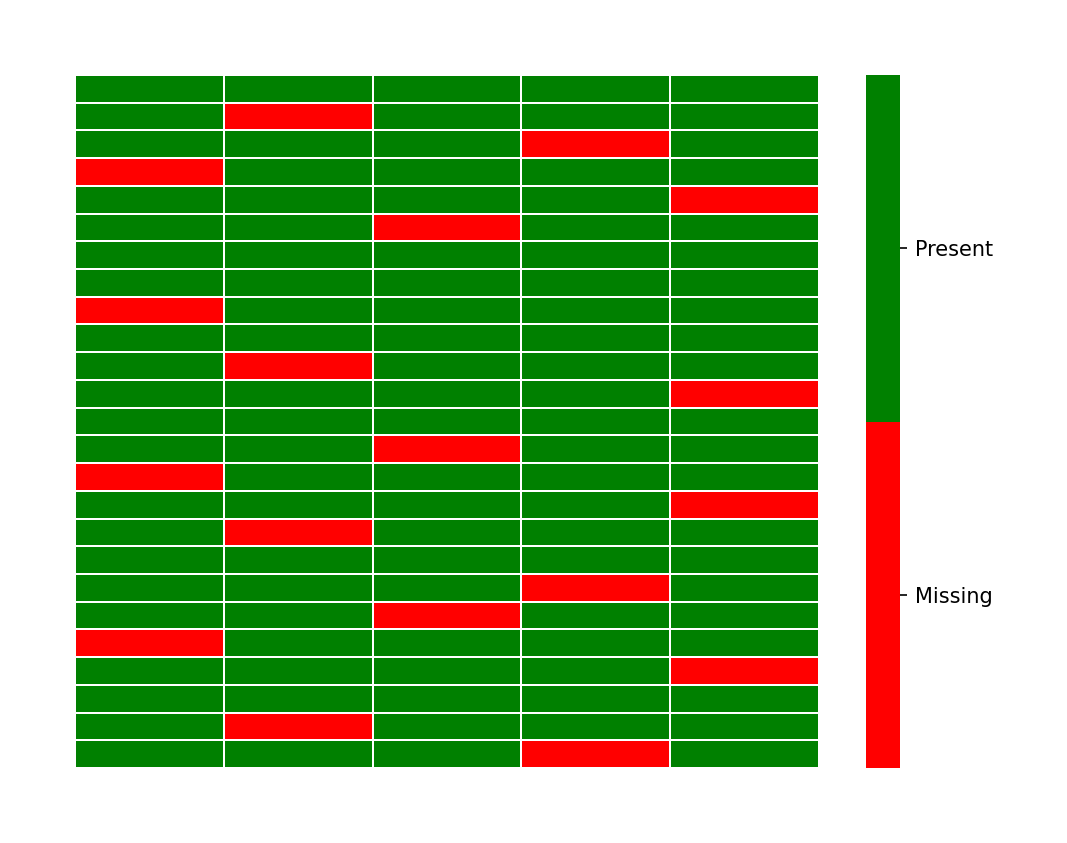
\includegraphics[width=0.5\linewidth]{MCAR_heatmap.png}
    \caption{Missing Completely At Random}
    \label{fig:mcar_heatmap}
\end{figure}

\textbf{Implication:} When datasets have an MCAR distribution, common statistical analysis methods, like estimation or regression, are still valid because the missingness does not introduce bias into the results. ~\cite{34}

\subsubsection{Missing At Random (MAR)}

Data are considered MAR when the probability of missingness depends only on observed variables and not on the missing values themselves. This pattern introduces a degree of predictability, which allows for effective correction using techniques such as conditional imputation or statistical modeling. ~\cite{24}

\begin{center}
$\Pr(R \mid y, X_{obs}, X_{mis}, \theta) = \Pr(R \mid y, X_{obs}, \theta)$
\end{center}

Where:
\begin{itemize}
\item R is the missingness indicator, where \( R_i = 1 \) if $y$ is missing, and \( R_i = 0 \) otherwise.
\item $y$ is the data vector (both observed and unobserved values).
\item $X_{obs}$ is the observed portion of the data.
\item $X_{mis}$ is the missing portion of the data.
\item $\theta$ are the parameters of the model generating the data.
\end{itemize}

\textbf{Example:} In a survey, income data may be missing more frequently among respondents with lower levels of education. The figure~\ref{fig:mar_heatmap} shows an example of a dataset with MAR missingness.

\begin{figure}[H]
\centering
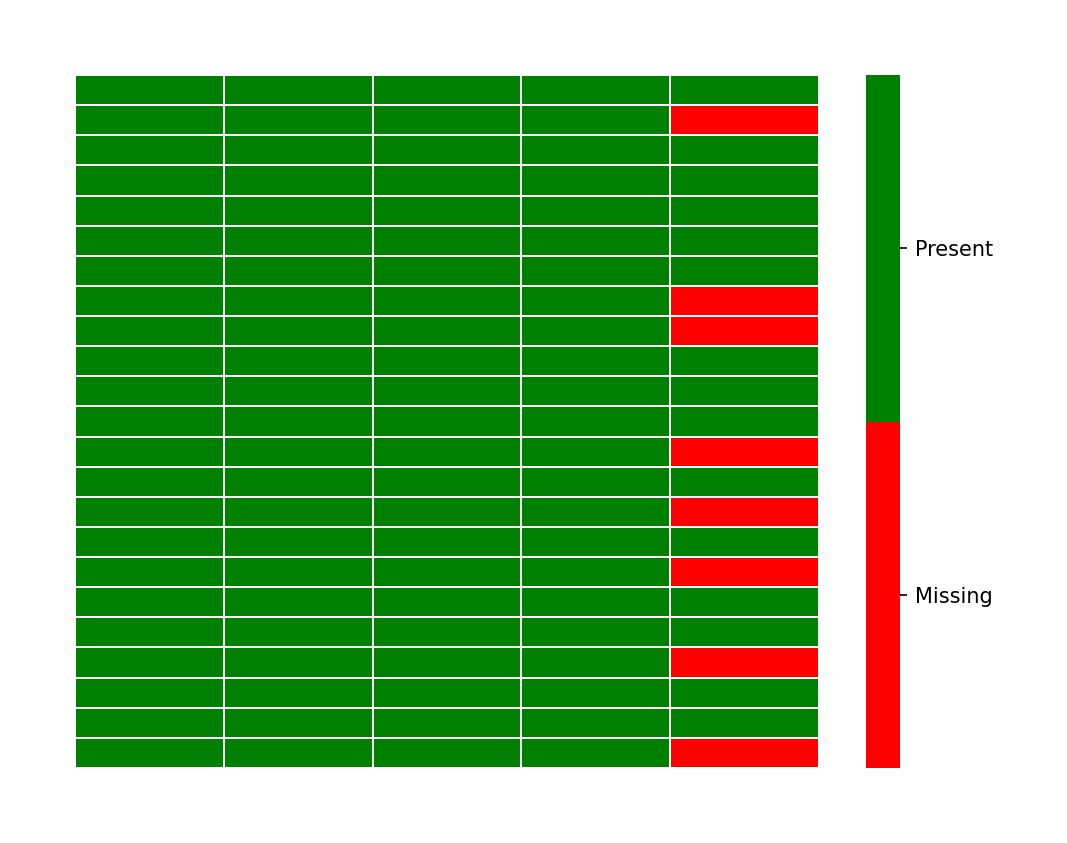
\includegraphics[width=0.5\linewidth]{MAR_heatmap.png}
\caption{Missing At Random}
\label{fig:mar_heatmap}
\end{figure}

\textbf{Implication:} Statistical methods that model the relationship between missingness and observed variables are appropriate for handling MAR datasets.

\subsubsection{Missing Not At Random (MNAR)}

Data are considered MNAR when the probability of missingness depends on unobserved variables or on the values that are themselves missing. This represents a more complex scenario, in which the missing data are systematically related to information that is not directly accessible. Handling MNAR often requires advanced modeling or external data sources. ~\cite{24}

\begin{center}
$f(M \mid Y_{obs}, Y_{mis}, \psi) = f(M \mid Y_{obs}, Y_{mis}, \psi)$
\end{center}

Where:
\begin{itemize}
    \item \( M \): is the missingness indicator, where \( M_i = 1 \) if the data point is missing and \( M_i = 0 \) otherwise.
    \item \( Y_{obs} \) is the observed values in the dataset.
    \item \( Y_{mis} \) is the missing values in the dataset (i.e., unobserved data).
    \item \( \psi \) are the parameters governing the missing data mechanism.
\end{itemize}


\textbf{Example:} In a survey, individuals with very high incomes may choose not to report their salary, resulting in systematic missingness. The figure~\ref{fig:mnar_heatmap} shows an example of a dataset with MNAR missingness.

\begin{figure}[H]
\centering
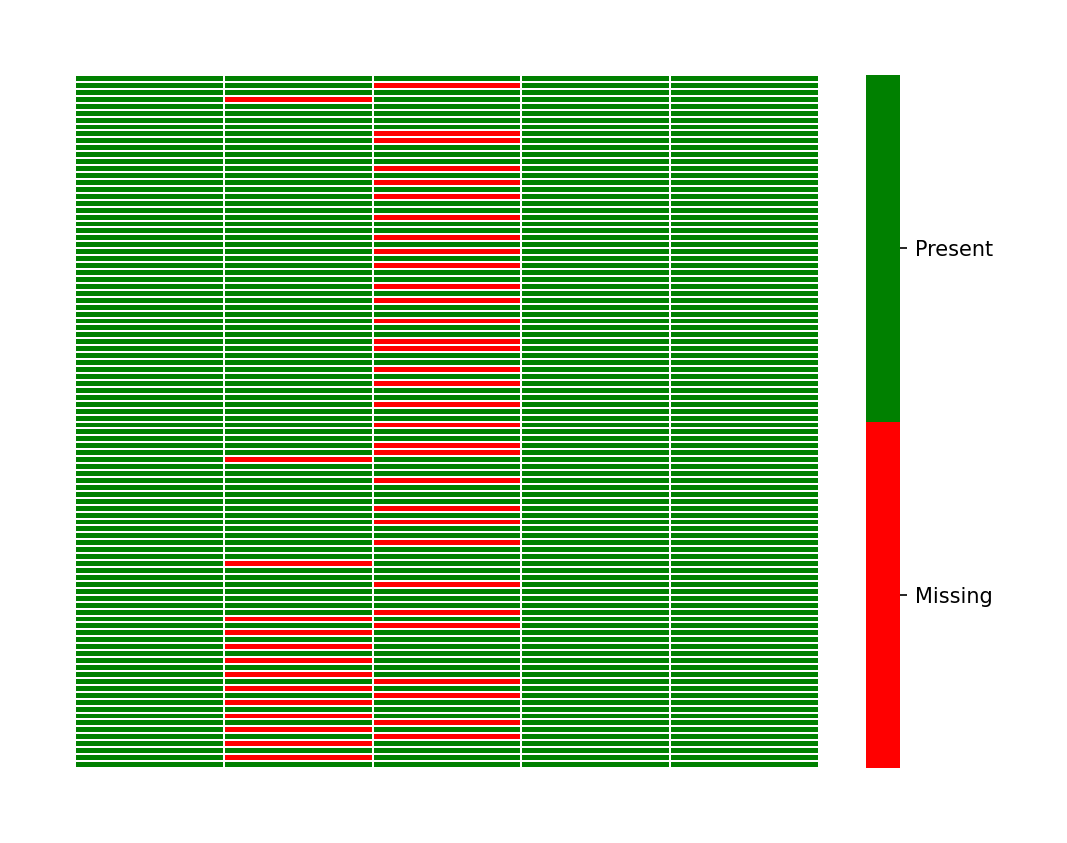
\includegraphics[width=0.5\linewidth]{MNAR_heatmap.png}
\caption{Missing Not At Random}
\label{fig:mnar_heatmap}
\end{figure}

\textbf{Implication:} Traditional methods can introduce significant bias. Special treatment or modeling is required to handle this type of missingness effectively.

\subsection{Traditional Methods for Handling Missing Data}

This section describes commonly used traditional techniques, such as deletion and imputation for handling missing data.

Handling missing data is a fundamental step in the data analysis pipeline. Two traditional approaches are commonly used to address this issue: listwise deletion and pairwise deletion. This section explains these two methods.

\subsubsection{Listwise Deletion}

This method removes all rows that contain any missing value. It is straightforward to implement and ensures that analyses are performed using only complete cases, simplifying statistical modeling.

However, its main disadvantage is the potential loss of a substantial amount of information, especially when missing data are widespread. Furthermore, it assumes that the data are MCAR—a condition that is rarely met in real-world scenarios—which can lead to biased results. ~\cite{3}. The figure~\ref{fig:listwise_deletion} compares the dataset before and after applying listwise deletion.

\begin{figure}[H]
\centering
\begin{subfigure}{0.48\textwidth}
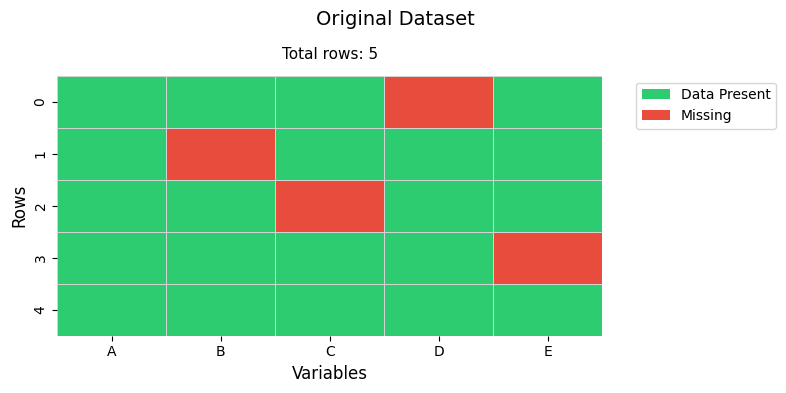
\includegraphics[width=\linewidth]{original_dataset.png}
\caption{Original Dataset}
\end{subfigure}
\hfill
\begin{subfigure}{0.48\textwidth}
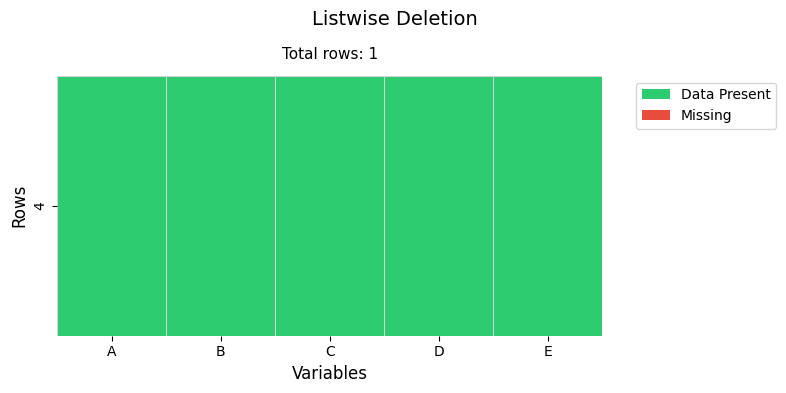
\includegraphics[width=\linewidth]{listwise_deletion.png}
\caption{Listwise Deletion}
\end{subfigure}
\caption{Listwise Deletion Example}
\label{fig:listwise_deletion}
\end{figure}


\subsubsection{Pairwise Deletion}

This approach is more flexible. Instead of removing entire rows, they impute values in the missing data cells. Pairwise deletion excludes missing values only from the specific calculations where they are needed.

It allows for more efficient use of available data but may introduce inconsistencies across analyses, as the sample size can vary between computations. Like listwise deletion, it assumes an MCAR distribution. ~\cite{3}. Figure~\ref{fig:pairwise_deletion} compares the dataset before and after applying pairwise deletion.

\begin{figure}[H]
\centering
\begin{subfigure}{0.48\textwidth}
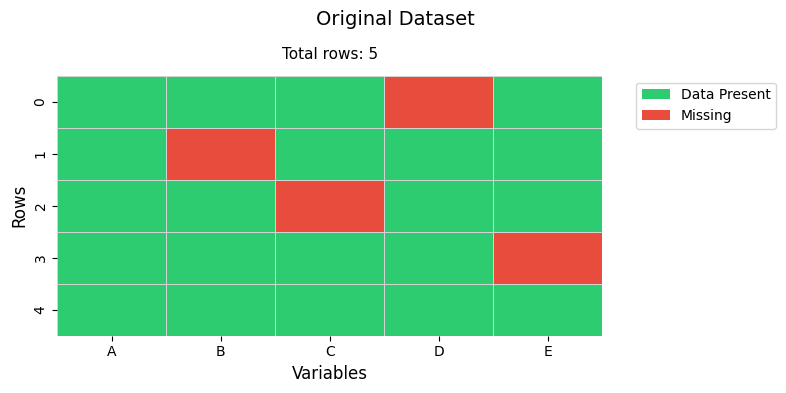
\includegraphics[width=\linewidth]{original_dataset.png}
\caption{Original Dataset}
\end{subfigure}
\hfill
\begin{subfigure}{0.48\textwidth}
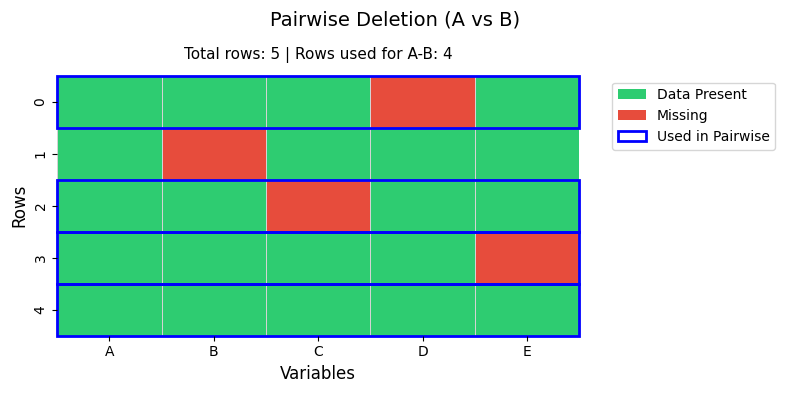
\includegraphics[width=\linewidth]{pairwise_deletion_(a_vs_b).png}
\caption{Pairwise Deletion}
\end{subfigure}
\caption{Pairwise Deletion Example}
\label{fig:pairwise_deletion}
\end{figure}

\subsubsection{Hot-deck Imputation}

Hot-deck imputation is a widely used imputation method that replaces missing values with observed values from the same dataset. Advantages of this method include its ease of application and the fact that it maintains real, existing data within the dataset. However, it also has drawbacks, like the potential for biased results if the replacement values are not representative enough. ~\cite{33}

Let’s consider the following dataset as an example:

\begin{table}[h]
\centering
\begin{tabular}{|c|c|c|}
\hline
\textbf{Name} & \textbf{Age} & \textbf{Score} \\
\hline
Alice & 20 & 85 \\
\hline
Bob & 27 & -- \\
\hline
Carol & 25 & 78 \\
\hline
David & 29 & 88 \\
\hline
\end{tabular}
\caption{Sample dataset for Hot-deck}
\label{tab:sample_data}
\end{table}

Using hot-deck imputation, we select another entry, in this case Carol, who has a comparable age, and use her score to fill in Bob’s missing value.

\subsubsection{Cold-deck Imputation}

Cold-deck imputation is very similar to hot-deck, with the key difference being that it uses external data to fill in missing values. This approach is particularly useful when working with a small dataset or when historical records of similar data are available. It can provide more reliable estimates in such cases. 

However, cold-deck imputation also comes with risks, especially if the external data is outdated or of poor quality. For example, if there has been a recent change in conditions, historical data might no longer be representative. 

Using the same dataset from the hot-deck example, imagine we have access to Bob’s scores from previous years. We could use those historical entries to generate a more accurate approximation of his missing score.

\subsubsection{Median Imputation}

The last imputation method we will explain here is Median Imputation. This approach uses the median of the representative data to fill in missing values. It allows you to reflect dependencies between variables and generate more realistic data. This becomes especially useful when dealing with MAR (Missing At Random) and MCAR (Missing Completely At Random) scenarios.\\

However, it assumes that the relationships between variables are linear, which can lead to biased models and suboptimal data generation.\\

\subsubsection{Limitations of Existing Approaches}

Summarizing the issues discussed, the traditional methods present the following limitations:

\begin{itemize}
    \item \textbf{MCAR Assumptions:} Most traditional methods assume data is MCAR, which rarely holds true in real-world scenarios.
    \item \textbf{Loss of Analytical Potential:} Removing rows or columns reduces the dataset size, potentially omitting valuable information and leading to less accurate models.
    \item \textbf{Skewed Results:} Systematic deletion of data can introduce bias when the missingness is not MCAR.
    \item \textbf{Variance problems:} Simple imputation methods do not reflect variability, failing to capture outliers or real distributional patterns.
\end{itemize}

\newpage
\section{Evaluation Metrics and Data Generation}

\subsection{Evaluation Metrics}

This section describes a scoring framework for evaluating missing data strategies, based on constraint satisfaction, missing value reduction, data retention, and preservation of key variables.

To compare algorithms and select the best one for handling missing data, I designed criteria that quantify the quality of the "cleaned" dataset. These criteria guided the algorithm development and form the foundation of the health scoring function. Key criteria include:

\begin{itemize}
    \item \textbf{Data Retention}: The algorithm should eliminate as much missing data as possible without compromising the integrity of the remaining data. Here, integrity means avoiding excessive loss of useful information or data relationships.
    \item \textbf{User Restrictions}: The algorithm must respect user-defined limits, prioritizing the preservation of critical elements or constraints specified by the user.
    \item \textbf{Preservation of Important Columns}: Columns marked as important should be preserved. Their deletion or having excessive missing values penalizes the score. This assumes that the dataset contains more rows than columns (\(n \gg p\)), so losing columns is worse than losing rows.
    \item \textbf{Structural Handling}: The algorithm should maintain the dataset's original structure (number of rows and columns).
\end{itemize}

\subsubsection{User's Restrictions}
This metric evaluates whether the "cleaned" dataset adheres to the constraints established by the user. Each fulfilled condition contributes proportionally to the score.

\begin{itemize}
    \item Minimum number of rows (\texttt{min\_rows})
    \item Minimum percent of rows (\texttt{min\_row\_percent})
    \item Maximum number of missing columns (\texttt{max\_missing})
    \item Minimum number of columns (\texttt{col\_threshold})
    \item Minimum percent of columns (\texttt{col\_relative\_threshold})
\end{itemize}

This metric accounts for 40\% of the final health score. Its formula is:
\[
\text{Constraint\_Score} = \left( \frac{\text{Accomplished Conditions}}{\text{Total Conditions}} \right) \times 40
\]

\subsubsection{Reduction of Missing Values}
This metric measures the algorithm's effectiveness at reducing the proportion of missing data. It accounts for 30\% of the final health score.

Formula:
\[
\text{Missing\_Score} =
\begin{cases}
30 & \text{if } \text{input\_missing} = 0 \\
\min\left(30, \frac{\text{input\_missing} - \text{output\_missing}}{\text{input\_missing}} \times 30 \right) & \text{otherwise}
\end{cases}
\]

Where \texttt{input\_missing} and \texttt{output\_missing} represent the number of missing values in the original and cleaned datasets, respectively.

\subsubsection{Data Retention}
This metric evaluates the proportion of rows and columns retained after cleaning, indicating how well the algorithm maintains the original structure. It accounts for 20\% of the final health score.\\

Formula:
\[
\text{Retention\_Score} = \left( \frac{\text{output\_rows}}{\text{input\_rows}} + \frac{\text{output\_cols}}{\text{input\_cols}} \right) \times 10
\]

This is a simple average of row and column retention, scaled to 20.

\subsubsection{Preservation of Important Columns}
This metric accounts for the final 10\% of the health score. It penalizes the algorithm if important columns are deleted or contain missing values after cleaning.\\

Formula:
\[
\text{Cols} =
\begin{cases}
0 & \text{if important columns are erased} \\
10 & \text{if they are complete} \\
\min\left(10, \frac{\text{input\_imp\_missing} - \text{output\_imp\_missing}}{\text{input\_imp\_missing}} \times 10 \right) & \text{otherwise}
\end{cases}
\]

\subsubsection{Total Health Score}
The overall health score is the sum of the four components:

\begin{itemize}
  \item \textbf{Health Score:}
  \[
  \text{Total\_Score} = \text{Constraint\_Score} + \text{Missing\_Score} + \text{Retention\_Score} + \text{Cols}
  \]
\end{itemize}

This system provides a standardized way to compare different strategies for handling missing data. Moreover, its automated implementation allows for easy replication of experiments. It also prints all relevant information used in the calculations, enabling the user to understand where potential issues may lie.

\subsubsection{Validation of Health Score via Extremes}

To validate the correctness of the health score, I designed two test cases to confirm that the scoring system properly assigns both its maximum and minimum values under ideal and worst-case conditions.

\paragraph{Perfect Score (100/100):}
\begin{itemize}
    \item \textbf{Erased Dataset:} 1000 rows and 100 columns with 200 values randomly erased.
    \item \textbf{Cleaned Dataset:} Identical to the erased dataset but with all missing values correctly restored.
\end{itemize}

\textbf{Score Breakdown:}
\begin{itemize}
    \item Constraint Adherence: 40/40 (all thresholds met)
    \item Missing Value Reduction: 30/30 (200 \textrightarrow 0)
    \item Data Retention: 20/20 (100\% rows/columns retained)
    \item Important Columns Bonus: 10/10 (all important columns preserved and complete)
\end{itemize}

\textbf{Total Score:} 100/100

\paragraph{Zero Score (0/100):}
\begin{itemize}
    \item \textbf{Erased Dataset:} 1000 rows and 100 columns with 200 missing values.
    \item \textbf{Cleaned Dataset:} Empty (0 rows, 0 columns).
\end{itemize}

\textbf{Score Breakdown:}
\begin{itemize}
    \item Constraint Adherence: 0/40 (too few rows/cols, too many missing)
    \item Missing Value Reduction: 0/30 (no improvement)
    \item Data Retention: 0/20 (everything lost)
    \item Important Columns Bonus: 0/10 (all important columns dropped)
\end{itemize}

\textbf{Total Score:} 0/100

These tests confirm that the scoring works as expected, rewarding complete, constraint-compliant datasets and penalizing excessive loss.

\subsection{Data Generation}

This section describes the synthetic data generation process for  MCAR
(Missing Completely At Random), MAR (Missing At Random), and MNAR (Missing
Not At Random) missingness patterns. The formal definitions and theoretical properties of these types are provided in Section 2.1.

\subsubsection{MCAR Data Generation}
The MCAR generator simulates missingness by randomly selecting entries in the dataset to mark as missing, in line with the MCAR definition (Section 2.1.1). The number of missing values per column follows a Binomial distribution with parameters \(n\) (total observations) and \(k\) (missingness proportion). ~\cite{24}
\[ 
K \sim \text{Binomial}(n, k)
\]

\subsubsection{Single Cutoff Method for MAR and MNAR}
For MAR and MNAR, the data generation uses a \textbf{single cutoff method}, where missingness depends on a threshold \(a\) applied to a predictor variable:

For MAR (see Section 2.1.2), missingness depends on observed variables. Given a predictor \(Y_2\), missing values in \(Y_1\) are generated with different probabilities above or below the cutoff \(a\).
For MNAR (see Section 2.1.3), missingness depends on the unobserved variable itself. Here, the missingness indicator depends on whether \(Y_1\) exceeds the cutoff \(a\).

Specifically, for both MAR and MNAR, the probability of missingness is defined as~\cite{24}:

\[
\begin{cases}
P(M=1 \mid U=1) = \pi_1 \\
P(M=1 \mid U=0) = \pi_2
\end{cases}
\]

where \(U=1\) if the corresponding variable exceeds the cutoff \(a\), and \(U=0\) otherwise.


\newpage
\section{Algorithms}
\subsection{Algorithmic Evolution}
At the start of the project, it was initially planned to develop a single algorithm to handle missing data. However, as the work progressed, we found that some simpler heuristics yielded better results than more complex approaches in certain scenarios. This insight led us to implement a broader suite of algorithms, offering a range of strategies to handle different patterns and densities of missingness.

\textbf{Implemented Versions:}
\begin{itemize}
    \item \textbf{v0.0:} The first functional prototype. It deletes rows with the highest number of missing values, using a simple weighting scheme for key columns.
    
    \item \textbf{v0.1:} Expands deletion criteria to include total missing values, minimum retention thresholds, and improved control over which rows are preserved.
    
    \item \textbf{v0.2:} Introduces a percentile-based architecture, analyzing the distribution of missing data across rows and columns.
    
    \item \textbf{v0.3:} Combines the logic from v0.1 and v0.2. It adds a scoring system, with normalization of missing counts and ranking for selection.
    
    \item \textbf{v0.4:} A fully vectorized implementation. It applies heuristics based on missing value concentration and considers column-wise standard deviation as an additional factor.
    
    \item \textbf{v0.5:} A consolidated and refined version. It introduces new column-level restrictions, adjusted weights, and improved overall robustness.
    
    \item \textbf{Branch and Bound (BnB):} A fundamentally different approach. It performs an exhaustive search of possible combinations of rows and columns to eliminate, aiming for an optimal submatrix with minimum information loss.
\end{itemize}

The algorithms were developed incrementally, which made it easier to manage growing complexity and evaluate the performance of each version over time.


\subsection{Description of the Algorithms}
\subsubsection{Algorithm v0.0}
This algorithm removes rows with the most missing values, penalizing missing data in important columns by applying a weight. It continues deleting rows until either a minimum number or percentage of rows remain or no missing values are left.\\
\textbf{Input}
\begin{itemize}
    \item \textbf{Dataset:} A .csv file (by default \texttt{output\_erased\_dataset.csv}) that contains the dataset.
    \item \textbf{Parameters:}
    \begin{itemize}
        \item \texttt{Min\_rows:} Minimum number of rows that must be preserved.
        \item \texttt{Min\_percent:} Minimum percentage of the original rows that must remain.
        \item \texttt{Important\_cols:} List of important columns.
        \item \texttt{Important\_weight:} Weight used to penalize missing values in \texttt{Important\_cols}.
        \item \texttt{Output:} Path to save the cleaned dataset.
    \end{itemize}
\end{itemize}


\textbf{Pseudocode}
\begin{algorithm}[H]
\caption{v0.0}
\begin{algorithmic}[1]
\Function{v0.0}{data, min\_rows, min\_percentage, important\_cols, weight}
    \State $original\_rows \gets$ \Call{CountRows}{data}
    \For{each row in data}
        \If{important\_cols is not empty \textbf{and} weight $>$ 1.0}
            \State $na\_important \gets$ \Call{CountNA}{row, important\_cols} $\times$ weight
            \State $na\_others \gets$ \Call{CountNA}{row, other\_columns}
            \State $row.na\_total \gets na\_important + na\_others$
        \Else
            \State $row.na\_total \gets$ \Call{CountNA}{row, all\_columns}
        \EndIf
    \EndFor
    \State \Call{SortRowsBy}{data, na\_total, descending}
    \While{true}
        \State $current\_rows \gets$ \Call{CountRows}{data}
        \State $current\_percentage \gets \frac{current\_rows}{original\_rows} \times 100$
        \If{$current\_rows \leq min\_rows$ \textbf{or} $current\_percentage \leq min\_percentage$ \textbf{or} \textbf{not} \Call{HasNAs}{data}}
            \State \textbf{break}
        \EndIf
        \State \Call{RemoveFirstRow}{data}
    \EndWhile
    \State \Return{cleaned\_dataset}
\EndFunction
\end{algorithmic}
\end{algorithm}

\textbf{Cost}
\begin{itemize}
    \item \textbf{Sorting:} $O(n \log n)$
    \item \textbf{Loop:} 
        \begin{itemize}
            \item Each iteration: remove row $O(n)$ + check NA $O(n \cdot m)$
            \item Total: $O(n^2 \cdot m)$
        \end{itemize}
    \item \textbf{Total:} $O(n \log n + n^2 \cdot m) \approx O(n^2 \cdot m)$ (worst case)
\end{itemize}

\subsubsection{Algorithm v0.1}
Starting from v0.0, this version takes into account the total number of missing values allowed in the dataset, stopping the removal process once the dataset meets specified thresholds on row count, percentage, or overall missing values.\\
\textbf{Input}
\begin{itemize}
    \item \textbf{Dataset:} A .csv file (by default \texttt{output\_erased\_dataset.csv}) that contains the dataset.
    \item \textbf{Parameters:}
    \begin{itemize}
        \item \texttt{Min\_rows:} Minimum number of rows that must be preserved.
        \item \texttt{Min\_percent:} Minimum percentage of the original rows that must remain.
        \item \texttt{Max\_missing:} Maximum number of missing values allowed in the final dataset.
        \item \texttt{Important\_cols:} List of important columns.
        \item \texttt{Important\_weight:} Weight used to penalize missing values in \texttt{Important\_cols}.
        \item \texttt{Output:} Path to save the cleaned dataset.
    \end{itemize}
\end{itemize}



\textbf{Pseudocode}
\begin{algorithm}[H]
\caption{v0.1}
\begin{algorithmic}[1]
\Function{v0.1}{data, min\_rows, min\_percentage, max\_na, important\_cols, weight}
    \State $original\_rows \gets$ \Call{CountRows}{data}
    \For{each row}
        \State $total\_na \gets$ \Call{CountNA}{row}
        \If{important\_cols \textbf{and} weight $>$ 1.0}
            \State $weighted\_na \gets$ (\Call{CountNA}{important\_cols} $\times$ weight) $+$ \Call{CountNA}{other\_columns}
        \Else
            \State $weighted\_na \gets total\_na$
        \EndIf
        \State $row.weighted\_na \gets weighted\_na$
    \EndFor
    \State \Call{SortRows}{data, \textit{by} weighted\_na \textit{descending}}
    \While{true}
        \State $current\_rows \gets$ \Call{CountRows}{data}
        \State $current\_percentage \gets \frac{current\_rows}{original\_rows} \times 100$
        \State $total\_na \gets$ \Call{Sum}{total\_na}
        \If{$(total\_na \leq max\_na)$ \textbf{or} $(current\_rows \leq min\_rows)$ \textbf{or} $(current\_percentage \leq min\_percentage)$}
            \State \textbf{break}
        \EndIf
        \If{data is empty}
            \State \textbf{break}
        \EndIf
        \State \Call{RemoveFirstRow}{data}
    \EndWhile
    \State \Return{cleaned\_dataset}
\EndFunction
\end{algorithmic}
\end{algorithm}

\textbf{Cost}
\begin{itemize}
    \item \textbf{Missing values calculation:} $O(n \cdot m)$ for computing both \texttt{na\_total} and \texttt{na\_weighted}.
    \item \textbf{Sorting:} $O(n \log n)$
    \item \textbf{Loop:} 
        \begin{itemize}
            \item Each iteration: calculate $total\_missing O(n)$ + delete row $O(n)$
            \item Total: $O(n^2 \cdot m)$
        \end{itemize}
    \item \textbf{Total:} $O(n \cdot m + n \log n + n^2) \approx O(n^2)$(worst case)
\end{itemize}

%%%%%%%%%%%%%%%%%%%%%%%%%%%%%%%%%%%%%%%%%%%%%%%

\subsubsection{Algorithm v0.2}
v0.2 takes a whole new approach, it applies a percentile cutoff on weighted missing values, filtering out rows above a calculated threshold to maintain a dataset with fewer missing values based on the distribution.

\textbf{Input}
\begin{itemize}
    \item \textbf{Dataset:} A .csv file (by default \texttt{output\_erased\_dataset.csv}) that contains the dataset.
    \item \textbf{Parameters:}
    \begin{itemize}
        \item \texttt{Percentile:} Minimum number of rows that must be preserved.
        \item \texttt{Important\_cols:} List of important columns.
        \item \texttt{Important\_weight:} Weight used to penalize missing values in \texttt{Important\_cols}.
        \item \texttt{Output:} Path to save the cleaned dataset.
    \end{itemize}
\end{itemize}



\textbf{Pseudocode}
\begin{algorithm}[H]
\caption{v0.2}
\begin{algorithmic}[1]
\Function{v0.2}{data, percentile, important\_cols, weight}
    \For{each row}
        \If{important\_cols \textbf{and} weight $>$ 1.0}
            \State weighted\_na $\gets$ (\textsc{CountNA}(important\_cols) $\times$ weight) $+$ \textsc{CountNA}(other\_columns)
        \Else
            \State weighted\_na $\gets$ \textsc{CountNA}(all\_columns)
        \EndIf
    \EndFor
    \State threshold $\gets$ \textsc{CalculatePercentile}(weighted\_na, percentile)
    \State filtered\_dataset $\gets$ \textsc{FilterRows}(data, weighted\_na $\leq$ threshold)
    \State \Return filtered\_dataset
\EndFunction
\end{algorithmic}
\end{algorithm}
\textbf{Cost}
\begin{itemize}
    \item \textbf{Missing values calculation:} $O(n \cdot m)$ 
    \item \textbf{Percentile calculation:} $O(n)$
    \item \textbf{Filter:} $O(n)$
    \item \textbf{Total:} $O(n \cdot m)$ (worst case)
\end{itemize}

%%%%%%%%%%%%%%%%%%%%%%%%%%%%%%%%%%%%%%%%%%%%%%%

\subsubsection{Algorithm v0.3}
This algorithm cleans by ranking rows based on a weighted combination of missing values and data quality, then uses binary search to find the optimal subset that satisfies user-defined constraints on minimum rows, maximum missing values, and minimum percentage retention.

\textbf{Input}
\begin{itemize}
    \item \textbf{Dataset:} A .csv file (by default \texttt{output\_erased\_dataset.csv}) that contains the dataset.
    \item \textbf{Parameters:}
    \begin{itemize}
        \item \texttt{Min\_rows:} Minimum number of rows that must be preserved.
        \item \texttt{Min\_percent:} Minimum percentage of the original rows that must remain.
        \item \texttt{Max\_missing:} Maximum number of missing values allowed in the final dataset.
        \item \texttt{Percentile:} Minimum number of rows that must be preserved.
        \item \texttt{Important\_cols:} List of important columns.
        \item \texttt{Important\_weight:} Weight used to penalize missing values in \texttt{Important\_cols}.
        \item \texttt{Output:} Path to save the cleaned dataset.
    \end{itemize}
\end{itemize}


\textbf{Pseudocode}
\begin{algorithm}[H]
\caption{v0.3}
\begin{algorithmic}[1]
\Function{v0.3}{data, percentile, min\_rows, max\_na, min\_percentage, important\_cols, weight}
    \State \textbf{// Step 1: Calculate weighted NA as in v0.2}
    \State weighted\_na $\gets$ \textsc{CalculateWeightedNA}(data, important\_cols, weight)
    
    \State ranks $\gets$ \textsc{AssignRank}(weighted\_na) \Comment{Highest NA gets rank 0}
    \State norm\_missing $\gets$ \textsc{Normalize}(weighted\_na) \Comment{Scale 0--1}
    \State norm\_rank $\gets$ \textsc{Normalize}(ranks) \Comment{Scale 0--1}
    
    \State combined\_score $\gets$ norm\_missing $+$ norm\_rank
    \State initial\_mask $\gets$ combined\_score $\leq$ \textsc{Percentile}(combined\_score, percentile)
    
    \If{min\_rows $>$ 0 \textbf{or} max\_na $>$ 0 \textbf{or} min\_percentage $>$ 0}
        \State sorted\_rows $\gets$ \textsc{SortRowsByScore}(combined\_score, ascending=true)
        \State \textbf{// Binary search to find max rows satisfying:}
        \State \textbf{// - rows $\geq$ min\_rows}
        \State \textbf{// - \% rows $\geq$ min\_percentage}
        \State \textbf{// - total\_na $\leq$ max\_na}
    \EndIf
    
    \State \Return filtered\_dataset
\EndFunction
\end{algorithmic}
\end{algorithm}

\textbf{Cost}
\begin{itemize}
    \item \textbf{Missing values calculation:} $O(n \cdot m)$
    \item \textbf{Sorting:} $O(n \log n)$
    \item \textbf{Binary search:} $O(\log n) \times O(n) = O(n \log n)$.
    \item \textbf{Total:} $O(n \cdot m + n \log n) \approx O(n \log n)$
\end{itemize}

%%%%%%%%%%%%%%%%%%%%%%%%%%%%%%%%%%%%%%%%%%%%%%%%

\subsubsection{Algorithm v0.4}
v0.4 introduces a multi-phase heuristic: it first removes columns with many missing values, then targets “zones” of rows with high missingness based on statistical deviations, and finally performs row removal until constrains are meet.

\textbf{Input}
\begin{itemize}
    \item \textbf{Dataset:} A .csv file (by default \texttt{output\_erased\_dataset.csv}) that contains the dataset.
    \item \textbf{Parameters:}
    \begin{itemize}
        \item \texttt{Min\_rows:} Minimum number of rows that must be preserved.
        \item \texttt{Min\_percent:} Minimum percentage of the original rows that must remain.
        \item \texttt{Max\_missing:} Maximum number of missing values allowed in the final dataset.
        \item \texttt{Important\_cols:} List of important columns.
        \item \texttt{Important\_weight:} Weight used to penalize missing values in \texttt{Important\_cols}.
        \item \texttt{std\_devs:} Standard deviations to define zones with high missingness.
        \item \texttt{col\_threshold:} Absolute minimum of columns to keep.
        \item \texttt{col\_relative\_threshold:} Minimum percentage of columns to keep.
        \item \texttt{Output:} Path to save the cleaned dataset.
    \end{itemize}
\end{itemize}

\textbf{Pseudocode}
\begin{algorithm}[H]
\caption{v0.4}
\begin{algorithmic}[1]
\Function{v0.4}{data, min\_rows, max\_na, min\_percentage, threshold\_cols, important\_cols, weight, std\_dev}
    \State min\_rows\_req $\gets \textsc{Max}\big(min\_rows, \min\_percentage \times \text{total\_rows}\big)$
    \State min\_cols\_req $\gets \textsc{Max}\big(threshold\_cols, \textstyle threshold\_columns \times \text{total\_columns}\big)$
    
    \State \textbf{// Phase 1: Column Removal}
    \State removable\_cols $\gets$ \textsc{NonImportantColumns}(data, important\_cols)
    \State \textsc{SortDescending}(removable\_cols, \textit{by} total\_NA)
    \While{total\_NA $>$ max\_na \textbf{and} remaining\_cols $>$ min\_cols\_req}
        \State \textsc{RemoveColumn}(column\_with\_most\_NA)
        \State \textsc{UpdateTotalNA}()
    \EndWhile
    
    \State \textbf{// Phase 2: Zone-Based Removal}
    \State mean\_na\_rows $\gets$ \textsc{Mean}(\textsc{NA\_per\_Row}(data))
    \State std\_dev\_na\_rows $\gets$ \textsc{StdDev}(\textsc{NA\_per\_Row}(data))
    \State high\_zone $\gets$ \{rows $|$ na\_row $>$ mean\_na\_rows $+$ std\_dev $\times$ std\_dev\_na\_rows\}
    \State \textsc{SortDescending}(high\_zone, \textit{by} importance\_weight)
    \State \textsc{RemoveRowsUntilConstraints}(high\_zone, min\_rows\_req, max\_na, min\_percentage)
    
    \State \textbf{// Phase 3: Global Removal}
    \If{constraints not met}
        \State \textsc{SortDescending}(all\_rows, \textit{by} importance\_weight)
        \State \textsc{RemoveRowsUntilConstraints}(all\_rows, min\_rows\_req, max\_na, min\_percentage)
    \EndIf
    
    \State \Return cleaned\_dataset
\EndFunction
\end{algorithmic}
\end{algorithm}

\textbf{Cost}
\begin{itemize}
    \item \textbf{Phase 1:} 
    \begin{itemize}
        \item Missing columns $O(n \cdot m)$ 
        \item Column order $O(m \log m)$
    \end{itemize}
    \item \textbf{Phase 2:}
    \begin{itemize}
        \item Zone identification $O(n \cdot m)$ 
        \item Weight calculation $O(|zone| \cdot m)$
        \item Sorting $O(|zone| \log |zone|)$
    \end{itemize}
    \item \textbf{Phase 3:}
    \begin{itemize}
        \item Weight calculation $O(n \cdot m)$ 
        \item Sorting $O(n \log n)$
        \item Iterative elimination $O(n^2)$
    \end{itemize}
    \item \textbf{Total:} $O(n \cdot m + n^2) \approx O(n^2)$ (worst case)
\end{itemize}

%%%%%%%%%%%%%%%%%%%%%%%%%%%%%%%%%%%%%%%%%%%%%%%%

\subsubsection{Algorithm v0.5}
Starting from v0.4, v0.5 continues with column and row removal, it uses standard deviations to handle missing data concentrations.

\textbf{Input}
\begin{itemize}
    \item \textbf{Dataset:} A .csv file (by default \texttt{output\_erased\_dataset.csv}) that contains the dataset.
    \item \textbf{Parameters:}
    \begin{itemize}
        \item \texttt{Min\_rows:} Minimum number of rows that must be preserved.
        \item \texttt{Min\_percent:} Minimum percentage of the original rows that must remain.
        \item \texttt{Max\_missing:} Maximum number of missing values allowed in the final dataset.
        \item \texttt{Important\_cols:} List of important columns.
        \item \texttt{Important\_weight:} Weight used to penalize missing values in \texttt{Important\_cols}.
        \item \texttt{std\_devs:} Standard deviations to define zones with high missingness.
        \item \texttt{col\_threshold:} Absolute minimum of columns to keep.
        \item \texttt{col\_relative\_threshold:} Minimum percentage of columns to keep.
        \item \texttt{Output:} Path to save the cleaned dataset.
    \end{itemize}
\end{itemize}

\textbf{Pseudocode}
\begin{algorithm}[H]
\caption{v0.5 Function: Column and Row Removal Based on Weighted NA}
\begin{algorithmic}[1]
\Function{v0.5}{data, min\_rows, max\_na, min\_percentage, threshold\_cols, important\_cols, weight}
    \State min\_rows\_req $\gets \textsc{Max}\big(min\_rows, \min\_percentage \times \text{total\_rows}\big)$
    \State min\_cols\_req $\gets \textsc{Max}\big(threshold\_cols, \textstyle threshold\_columns \times \text{total\_columns}\big)$

    \State \textbf{// Phase 1: Column Removal}
    \State removable\_cols $\gets$ \textsc{NonImportantColumns}(data, important\_cols)
    \State \textsc{SortDescending}(removable\_cols, \textit{by} total\_NA)
    \While{total\_NA $>$ max\_na \textbf{and} remaining\_cols $>$ min\_cols\_req}
        \State \textsc{RemoveColumn}(column\_with\_most\_NA)
        \State \textsc{UpdateTotalNA}()
    \EndWhile

    \State \textbf{// Phase 2: Row Removal}
    \While{total\_NA $>$ max\_na \textbf{and} remaining\_rows $>$ min\_rows\_req}
        \State row\_weight $\gets$ (NA\_in\_important\_cols $\times$ weight) $+$ NA\_in\_other\_cols
        \State \textsc{RemoveRow}(row\_with\_max\_weight)
        \State \textsc{UpdateTotalNA}()
    \EndWhile

    \State \Return cleaned\_dataset
\EndFunction
\end{algorithmic}
\end{algorithm}

\textbf{Cost}
\begin{itemize}
    \item \textbf{Phase 1:} 
    \begin{itemize}
        \item Missing columns $O(n \cdot m)$ 
        \item Column sorting $O(m \log m)$
        \item Iterative elimination $O(k \cdot n \cdot m)$
    \end{itemize}
    \item \textbf{Phase 2:}
    \begin{itemize}
        \item Weight calculation $O(n \cdot m)$ 
        \item Iterative elimination $O(r \cdot n \cdot m)$
    \end{itemize}
    \item \textbf{Total:}  $O(n \cdot m \cdot (k + r)) \approx O(n^2 \cdot m)$ (worst case)
\end{itemize}


%%%%%%%%%%%%%%%%%%%%%%%%%%%%%%%%%%%%%%%%%%%%%%%%

\subsubsection{Branch and Bound}
This method exhaustively searches combinations of rows and columns to find an optimal subset minimizing information loss, trading computational efficiency for potentially better cleaning results.

\textbf{Input}
\begin{itemize}
    \item \textbf{Dataset:} A .csv file (by default \texttt{output\_erased\_dataset.csv}) that contains the dataset.
    \item \textbf{Parameters:}
    \begin{itemize}
        \item \texttt{Min\_rows:} Minimum number of rows that must be preserved.
        \item \texttt{Min\_percent:} Minimum percentage of the original rows that must remain.
        \item \texttt{col\_threshold:} Absolute minimum of columns to keep.
        \item \texttt{max\_col\_missing:} Number of missing values allowed per column.
        \item \texttt{Output:} Path to save the cleaned dataset.
    \end{itemize}
\end{itemize}


\textbf{Pseudocode}
\begin{algorithm}[H]
\caption{Branch and Bound (BnB)}
\begin{algorithmic}[1]
\Function{BnB}{data, min\_rows, min\_columns, max\_na\_per\_column}
    \State best\_solution $\gets$ \textbf{None}
    \State best\_cost $\gets$ $\infty$
    \State priority\_queue $\gets$ [(\Call{LowerBound}{initial\_state}, initial\_state)]
    
    \While{priority\_queue not empty}
        \State state $\gets$ \Call{ExtractMin}{priority\_queue}
        \If{state.lower\_bound $\geq$ best\_cost}
            \State \textbf{continue} \Comment{Prune this branch}
        \EndIf
        
        \If{state meets constraints (min\_rows, min\_columns, max\_na\_per\_column)}
            \If{state.cost $<$ best\_cost}
                \State best\_solution $\gets$ state
                \State best\_cost $\gets$ state.cost
            \EndIf
        \Else
            \State child\_row $\gets$ \Call{RemoveRow}{state, worst\_row\_index}
            \State child\_col $\gets$ \Call{RemoveColumn}{state, worst\_column\_index}
            \State \Call{AddToQueue}{priority\_queue, child\_row}
            \State \Call{AddToQueue}{priority\_queue, child\_col}
        \EndIf
    \EndWhile
    \State \Return best\_solution
\EndFunction

\vspace{1em}

\Function{LowerBound}{state}
    \State rows\_to\_remove $\gets \max(0,\ \text{state.current\_rows} - \text{min\_rows})$
    \State cols\_to\_remove $\gets \max(0,\ \text{state.current\_columns} - \text{min\_columns})$
    \State invalid\_cols $\gets$ \Call{CountColumnsWithNA}{state, max\_na\_per\_column}
    \State cols\_to\_remove $\gets \max(\text{cols\_to\_remove},\ \text{invalid\_cols})$
    \State \Return rows\_to\_remove $+$ cols\_to\_remove
\EndFunction
\end{algorithmic}
\end{algorithm}

\textbf{Monotonicity}  
Monotonicity refers to the property that, as we move deeper into a search tree (from parent to child nodes), the lower bound of the cost function can only worsen—in the case of minimization problems, it can only increase. Formally, if node \(A\) is a parent of node \(B\), then it must hold that \(\text{LowerBound}(A) \leq \text{LowerBound}(B)\). This condition is crucial because, without it, we risk pruning branches of the tree that might actually contain the optimal solution. In other words, if monotonicity is not guaranteed, the search algorithm could mistakenly eliminate a path that later improves and leads to a better result~\cite{34}.

\textbf{Connection to Optimality}  
Monotonicity is a key factor for preserving optimality because it guarantees that no better solutions are overlooked due to pruning. This reduces computational cost without sacrificing correctness~\cite{34}.

\textbf{Formula:}
\[
\text{Cost}_{\text{total}} = r_v + c_v + \text{min\_additional\_rows} + \max(\text{min\_additional\_cols}, \text{violating\_cols})
\]
Where:
\begin{itemize}
    \item $r_v$: nummber of erased columns.
    \item $c_v$: nummber of erased rows.
    \item \texttt{min\_additional\_rows}: ramaining rows to erase to reach \texttt{min\_rows}.
    \item \texttt{min\_additional\_cols}: ramaining columns to erase to reach \texttt{min\_cols}.
    \item \texttt{violating\_cols}: columns that violare the minimum \% per row
\end{itemize}

Suppose the initial dataset has 1000 rows and 50 columns. The user-specified constraints
are: 
\begin{itemize}
    \item $r_v = 0$
    \item $c_v = 0$
    \item 800 must be retained $\Rightarrow$ 200 rows to erase.
    \item 40 columns must remain $\Rightarrow$ 10 columns to erase
    \item 20\% of missing values per column $\Rightarrow$ 5 columns to erase.
\end{itemize}

The cost we get is 
\[
\text{Cost}_{\text{0}} = 0 + 0 +200 + \max(10, 5) = 210
\]

Entonces:
\[
\text{Cost}_{\text{total}} = 0 + 0 + 0 + \max(0, 5) = 5
\]

This is the lower bound that the cost can get. As we erase rows and columns, $r_v + c_v$ grows, and \texttt{min\_additional\_rows}, \texttt{min\_rows} and  will decrease. Let's see this with the next step where we erase a row. 

\begin{itemize}
    \item $r_v = 1$
    \item $c_v = 0$
    \item 800 must be retained $\Rightarrow$ 199 rows to erase.
    \item 40 columns must remain $\Rightarrow$ 10 columns to erase
    \item 20\% of missing values per column $\Rightarrow$ 5 columns to erase.
\end{itemize}

The cost we get is 
\[
\text{Cost}_{\text{0}} = 1 + 0 +199 + \max(10, 5) = 210
\]

We can see that monotonicity holds: $210 \leq 210$

\textbf{Cost}
\begin{itemize}
    \item \textbf{Total:} $O(2^{(n+m)})$ (worst case)
\end{itemize}

\subsection{UI Functionality and Integration}
As a complementary part of the project, I chose to develop a simple user interface using the Python library \texttt{Tkinter}. Although it wasn't part of the original thesis plan, the idea emerged from an interesting conversation with a Master's student.

The interface is structured in a modular form, allowing the user to follow a logical flow from the welcoming screen to the result visualization.

\subsubsection{General Structure}
\textbf{Welcoming Screen} \\
The first screen presents a simple design with a start button that gives access to the data input section.

\begin{figure}[H]
\centering
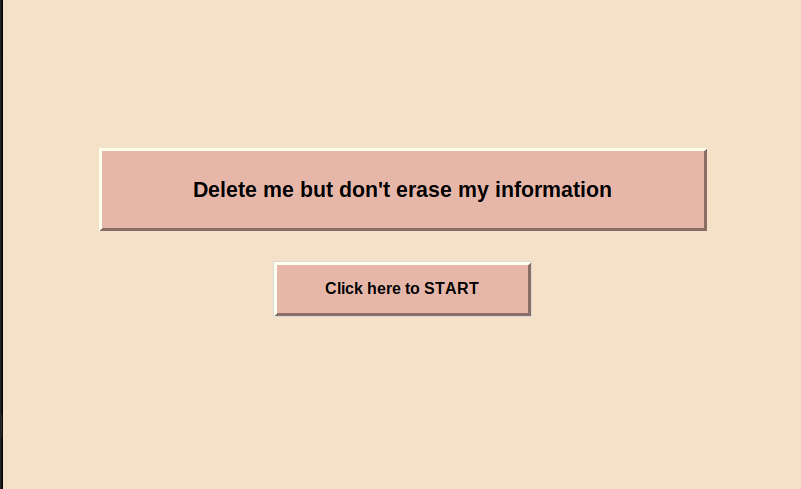
\includegraphics[width=0.5\linewidth]{Welcome.png}
\caption{Welcoming Screen}
\end{figure}

\textbf{Data Input Screen} \\
In this screen, the user can choose between two options to run the algorithms:
\begin{itemize}
    \item \textbf{Generate data:} Allows the user to generate synthetic data and opens the data generator screen.
    \item \textbf{My own data:} Lets the user select a document from the local system; once selected, it redirects to the algorithm selection screen.
\end{itemize}

\begin{figure}[H]
\centering
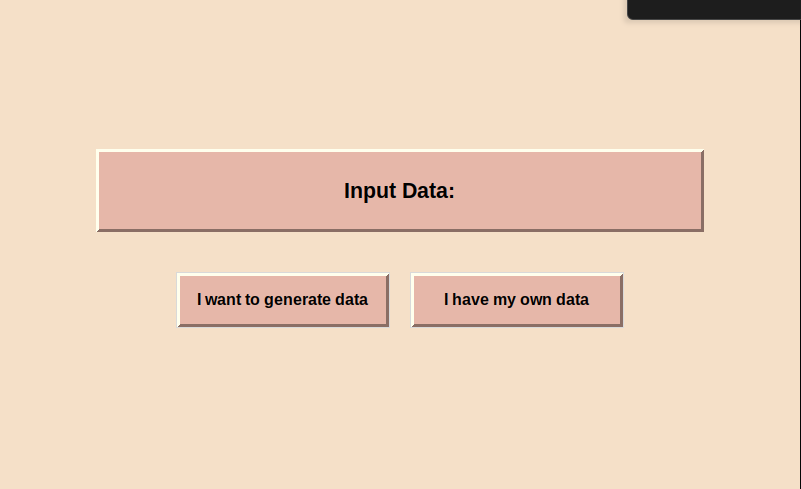
\includegraphics[width=0.5\linewidth]{Data_input.png}
\caption{Data Input Screen}
\end{figure}

\textbf{Data Pattern Generator} \\
In this screen, the user chooses between three buttons (MCAR, MAR, MNAR). Once selected and the necessary parameters are input, the screen redirects to the algorithm selection screen.

\begin{figure}[H]
\centering
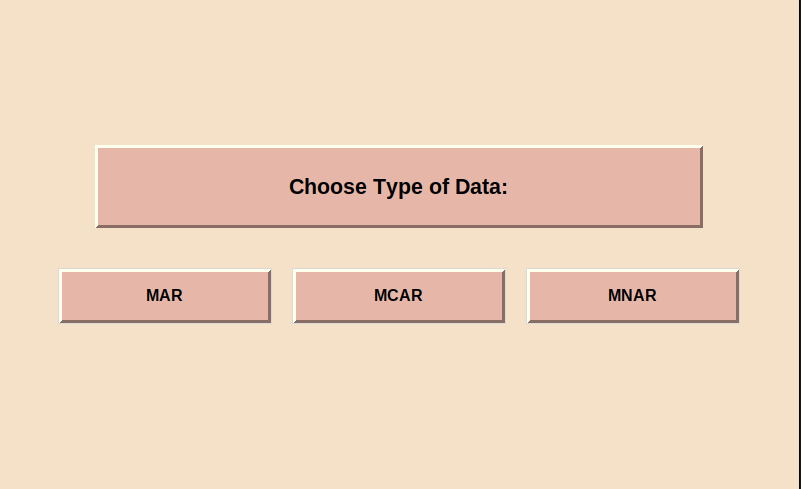
\includegraphics[width=0.5\linewidth]{MCAR_MNAR_MAR.png}
\caption{Data Pattern Generator Screen}
\end{figure}

\textbf{Algorithm Selection Screen} \\
Here, the user inputs all the required parameters to run the algorithms. Upon pressing "Start", the algorithms are executed, and the user is redirected to the results screen.

\begin{figure}[H]
\centering
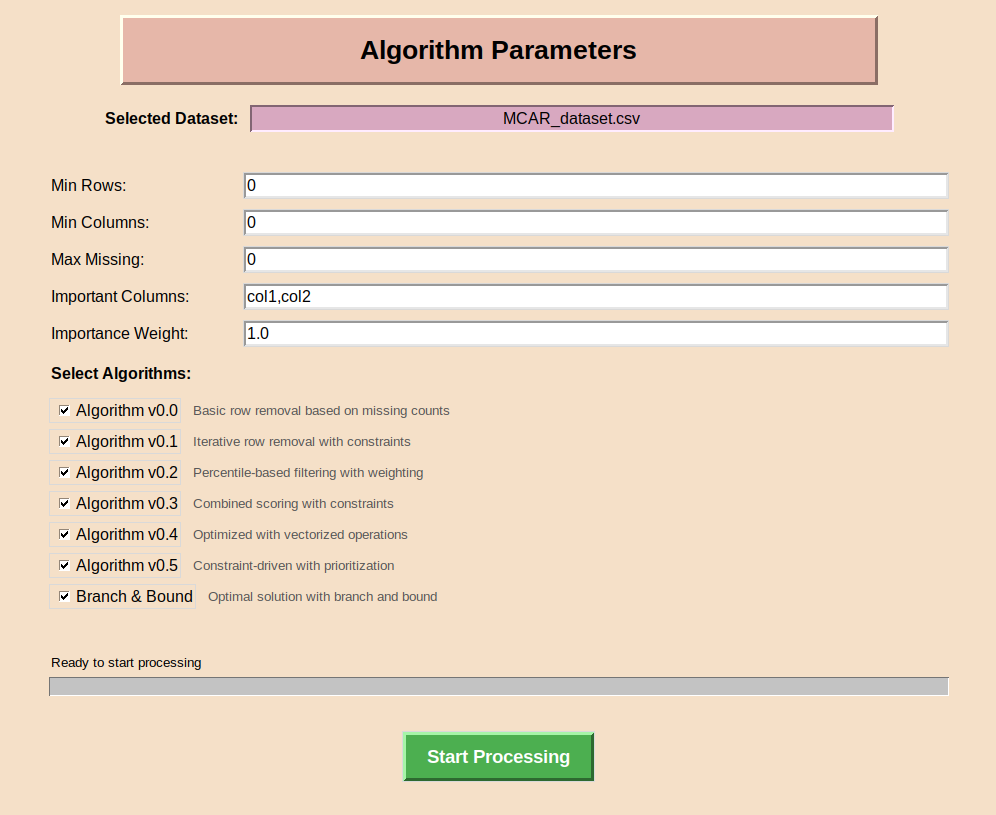
\includegraphics[width=0.5\linewidth]{ALG_INP.png}
\caption{Algorithm Selection Screen}
\end{figure}

\textbf{Result Screen} \\
In this window, the results are displayed in the form of scores. The user has the option to return to the Welcoming Screen, restarting the entire flow.

\begin{figure}[H]
\centering
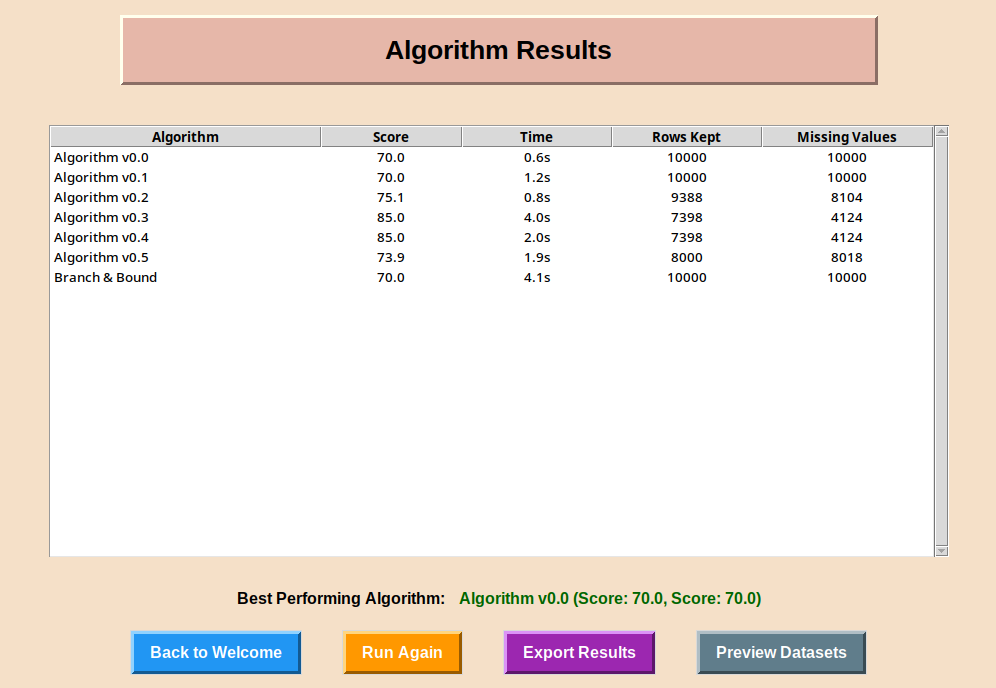
\includegraphics[width=0.5\linewidth]{Results.png}
\caption{Result Screen}
\end{figure}

\subsection{Technologies and Tools Used}

During the development of the project, a variety of tools and technologies were used to implement, execute, and visualize the algorithms. The following list highlights the most relevant ones:

\begin{itemize}
    \item \textbf{Python 3.10:} The main programming language used, selected for its versatility, readable syntax, and large community support.
    
    \item \textbf{NumPy and Pandas:} Essential libraries for handling datasets, including loading, transforming, and analyzing data.
    
    \item \textbf{Matplotlib and Seaborn:} Key tools for generating visualizations, particularly heatmaps, which were crucial for analyzing the structure and restoration of missing data.
    
    \item \textbf{Tkinter:} Python’s standard GUI library, used to develop a simple interface for running the algorithms and loading or generating data.
    
    \item \textbf{CUDA and GPU Acceleration:} All data generation scripts were optimized for GPU execution, enabling realistic matrix creation times and eliminating performance bottlenecks.
    
    \item \textbf{Virtual Environment:} As a best practice in Python projects, a virtual environment was used to manage project dependencies in an isolated and controlled manner.
\end{itemize}

\newpage
\section{Experimentation and Results}

\subsection{Experimental Setup}
To evaluate the effectiveness of the developed algorithms, a synthetic environment was created to simulate various missing data scenarios. This approach was motivated by two main reasons. First, synthetic datasets offer full control over key aspects such as size, distribution, and the exact percentage and pattern of missing values. Second, in real-world datasets, the nature and distribution of missing data are often unknown, making it difficult to objectively compare the performance of imputation or deletion methods.

Each experiment involves generating an original dataset, introducing missing data according to specific patterns, applying all algorithms to produce results, and evaluating these results using quantitative metrics.

The experiments were automated using a Bash script that executes six sequential steps. All outputs from each run are saved in a directory named \texttt{/logs}, including execution times, heatmaps, and the generated \texttt{.csv} files. This setup ensures experiment reproducibility and supports drawing reliable conclusions.

\subsubsection{Generation of Complete Datasets}
All the experiments are based on synthetic datasets generated from scratch. Each dataset has a dimension of $10^5$ rows and $10^4$ columns and includes both numerical and categorical variables generated randomly. These datasets simulate real-world datasets with high dimensionality and data diversity.

\subsubsection{Identification of Important Columns} 
To evaluate the algorithms' capacity to preserve critical variables, the first 100 columns (col\_1 to col\_100) are designated as important. These columns are assigned greater weight in the evaluation: if they are eliminated or retain many missing values, the algorithm receives a high penalty.

\subsubsection{Simulation of Missing Values}
For this experiment, we used nine test cases that evenly cover all three missing data distributions: MCAR, MAR, and MNAR. Each pattern was applied using custom GPU-based Python scripts\footnote{MCAR: \texttt{erase\_generator\_MCAR\_GPU.py}; MAR: \texttt{erase\_generator\_MAR\_GPU.py}; MNAR: \texttt{erase\_generator\_MNAR\_GPU.py}.}. The use of GPU implementations helped maintain high efficiency even with large-scale data. Each case includes specific parameters such as the number of affected columns, percentage of missing data, etc. Each case will be thoroughly explained in the next section.
\subsubsection{Algorithm Application}
Once the datasets were generated, each of the tested algorithms was applied:
\begin{itemize}
    \item \textbf{Versions 0.0 to 0.5:} Greedy algorithms.
    \item \textbf{Branch and Bound:} An alternative implementation used as a baseline.
\end{itemize}
Each algorithm received the necessary inputs specific to its logic.

\subsubsection{Visualization}
To further clarify the results, not only was a health score computed to directly compare all algorithms, but heatmaps were also generated to visualize the datasets before and after processing. These visualizations helped us better understand the behavior of the algorithms.

\subsubsection{Result Evaluation}
Finally, each result was evaluated using the algorithm and criteria described in Sections 3.3 and 5.3.

\subsection{Experimental Case Descriptions}
Each case is designed to represent one of the three distributions (MCAR, MNAR, or MAR), with parameters carefully chosen to reflect diverse scenarios and varying levels of difficulty. For each case, we will provide the selected parameters, a brief description, and the rationale behind the choices. 
\subsubsection{Case 1: MCAR - 10\%}
\begin{itemize}
    \item \textbf{Parameters:} \texttt{--num\_columns 50 --percentage 10}
    \item \textbf{Description:} Missing values are introduced in 10\% of the cells across 50 randomly selected columns.
    \item \textbf{Justification:} This scenario simulates a common situation where data is lost in a non-systematic manner.
\end{itemize}

\subsubsection{Case 2: MCAR - 25\%}
\begin{itemize}
    \item \textbf{Parameters:} \texttt{--num\_columns 100 --percentage 25}
    \item \textbf{Description:} Missing values are introduced in 25\% of the cells across 100 randomly selected columns.
    \item \textbf{Justification:} This scenario simulates a more severe loss of data, though still occurring in a non-systematic way. It allows us to evaluate the algorithm's ability to adapt to harsher conditions.
\end{itemize}

\subsubsection{Case 3: MAR Dependency in Three Reference Columns}
\begin{itemize}
    \item \textbf{Parameters:} \texttt{--reference\_column col\_501 col\_502 col\_503},\\
    \texttt{--target\_column col\_1 col\_2 col\_3},\\
    \texttt{--cutoff 5000 5000 5000},\\
    \texttt{--pi\_high 0.3 0.3 0.3},\\
    \texttt{--pi\_low 0.1 0.1 0.1}
    
    \item \textbf{Description:} The missingness in three target columns depends on three reference columns. Being over the cutoff increases the probability of data loss.
    \item \textbf{Justification:} MAR is more common than MCAR in the real world. In this case we introduce a moderate dependency, simulating situations such as the omission of age or income.  
\end{itemize}

\subsubsection{Case 4: MAR – Dependency on Five Reference Columns}
\begin{itemize}
    \item \textbf{Parameters:} \texttt{--reference\_column col\_601...col\_605},\\
    \texttt{--target\_column col\_11...col\_15},\\
    \texttt{--cutoff 7500...7500},\\
    \texttt{--pi\_high 0.6...0.6},\\
    \texttt{--pi\_low 0.2...0.2}
    
    \item \textbf{Description:} The missingness in five target columns depends on five reference columns. In this case, the probability of missingness is significantly higher than in previous cases.
    
    \item \textbf{Justification:} This case emulates a complex dependency. It is used to test the sensitivity of the algorithm to non-trivial variable relationships. We aim to evaluate whether, under higher levels of missing data, some form of skewing is introduced.
\end{itemize}

\subsubsection{Case 5: MNAR – Moderate Dependency}
\begin{itemize}
    \item \textbf{Parameters:} \texttt{--column col\_21 col\_22 col\_23},\\
    \texttt{--cutoff 6000},\\
    \texttt{--pi\_high 0.4},\\
    \texttt{--pi\_low 0.15}
    
    \item \textbf{Description:} The missingness pattern depends on the value within each column.
    
    \item \textbf{Justification:} This case simulates situations where data is missing due to extreme values, sensitivity, or anomalies. It is characteristic of psychological or financial contexts, where individuals tend to withhold sensitive information.
\end{itemize}

\subsubsection{Case 6: MNAR – Strong Dependency}
\begin{itemize}
    \item \textbf{Parameters:} \texttt{--column col\_31...col\_35},\\
    \texttt{--cutoff 8000},\\
    \texttt{--pi\_high 0.7},\\
    \texttt{--pi\_low 0.3}
    
    \item \textbf{Description:} We follow the same pattern as in Case 5, but with more columns and stronger conditional probabilities.
    
    \item \textbf{Justification:} This case simulates challenging situations where missing data is concentrated in critical ranges. Once again, it aims to test the robustness of the algorithms under harsher conditions.
\end{itemize}

\subsubsection{Case 7: MCAR – 15\%}
\begin{itemize}
    \item \textbf{Parameters:} \texttt{--num\_columns 75 --percentage 15}
    
    \item \textbf{Description:} Missing values are introduced in 15\% of the cells across 75 randomly selected columns.
    
    \item \textbf{Justification:} This scenario represents an intermediate case between Case 1 and Case 2, balancing missingness severity for comparative analysis.
\end{itemize}

\subsubsection{Case 8: MAR – Dependency on Four Reference Columns}
\begin{itemize}
    \item \textbf{Parameters:} \texttt{--reference\_column col\_701...col\_704},\\
    \texttt{--target\_column col\_41...col\_44},\\
    \texttt{--cutoff 6500...6500},\\
    \texttt{--pi\_high 0.5...0.5},\\
    \texttt{--pi\_low 0.25...0.25}
    
    \item \textbf{Description:} The missingness in four target columns depends on four reference columns.
    
    \item \textbf{Justification:} This scenario represents an intermediate case between Case 3 and Case 4, balancing missingness severity and complexity.
\end{itemize}

\subsubsection{Case 9: MNAR – Complex Dependency}
\begin{itemize}
    \item \textbf{Parameters:} \texttt{--column col\_51...col\_54},\\
    \texttt{--cutoff 7000},\\
    \texttt{--pi\_high 0.6},\\
    \texttt{--pi\_low 0.2}
    
    \item \textbf{Description:} This case represents an MNAR pattern where multiple columns exhibit missingness based on internal values, following defined conditional probabilities.
    
    \item \textbf{Justification:} This scenario serves as an intermediate case between Case 5 and Case 6, offering a balance between the severity and complexity of missingness.
\end{itemize}


\subsection{Comparative Analysis}
In this section, we compare the results obtained by the different algorithms on the cases defined in Section 5.2. The scores are based on the evaluation criteria described in Section 3.1. For each case, we include the following:

\begin{itemize}
    \item A score table for all algorithms
    \item Observations about the best- and worst-performing algorithms
    \item Commentary on the heatmaps
\end{itemize}

\subsubsection{Case 1: MCAR – 10\%}

\textbf{Score Table:}

\begin{table}[h]
\centering
\caption{Scores by algorithm, Case 1}
\label{tab:score_algorithms_case1}
\begin{tabular}{|c|c|c|c|c|c|c|c|c|}
\hline
Algorithm & v0.0 & v0.1 & v0.2 & v0.3 & v0.4 & v0.5 & BnB & Average \\
\hline
Score & 64.4 & 62.3 & 59.9 & 59.3 & 83.6 & 83.3 & 60.0 & \textbf{67.97} \\
\hline
\end{tabular}
\end{table}

\textbf{Observations}\\
The highest-performing algorithm is v0.4, with a health score of 83.6. The most notable characteristics of the component parts of the health score are Constraint Adherence and Data Retention, which have very high results: 40/40 and 19.6/20, respectively. The lowest score is from v0.3 (59.3), due to low Constraint Adherence (24/40) and Columns Bonus (0.0/10). The total performance gap between the best and worst scores is 27 points, indicating a relevant difference in effectiveness. Curiously, BnB, an exhaustive method, underperforms, suggesting that algorithmic complexity does not guarantee better results.

\textbf{Heatmaps}\\
We begin by examining the input dataset to ensure that the missingness pattern corresponds to a uniform MCAR distribution, as intended.

\begin{figure}[H]
    \centering
    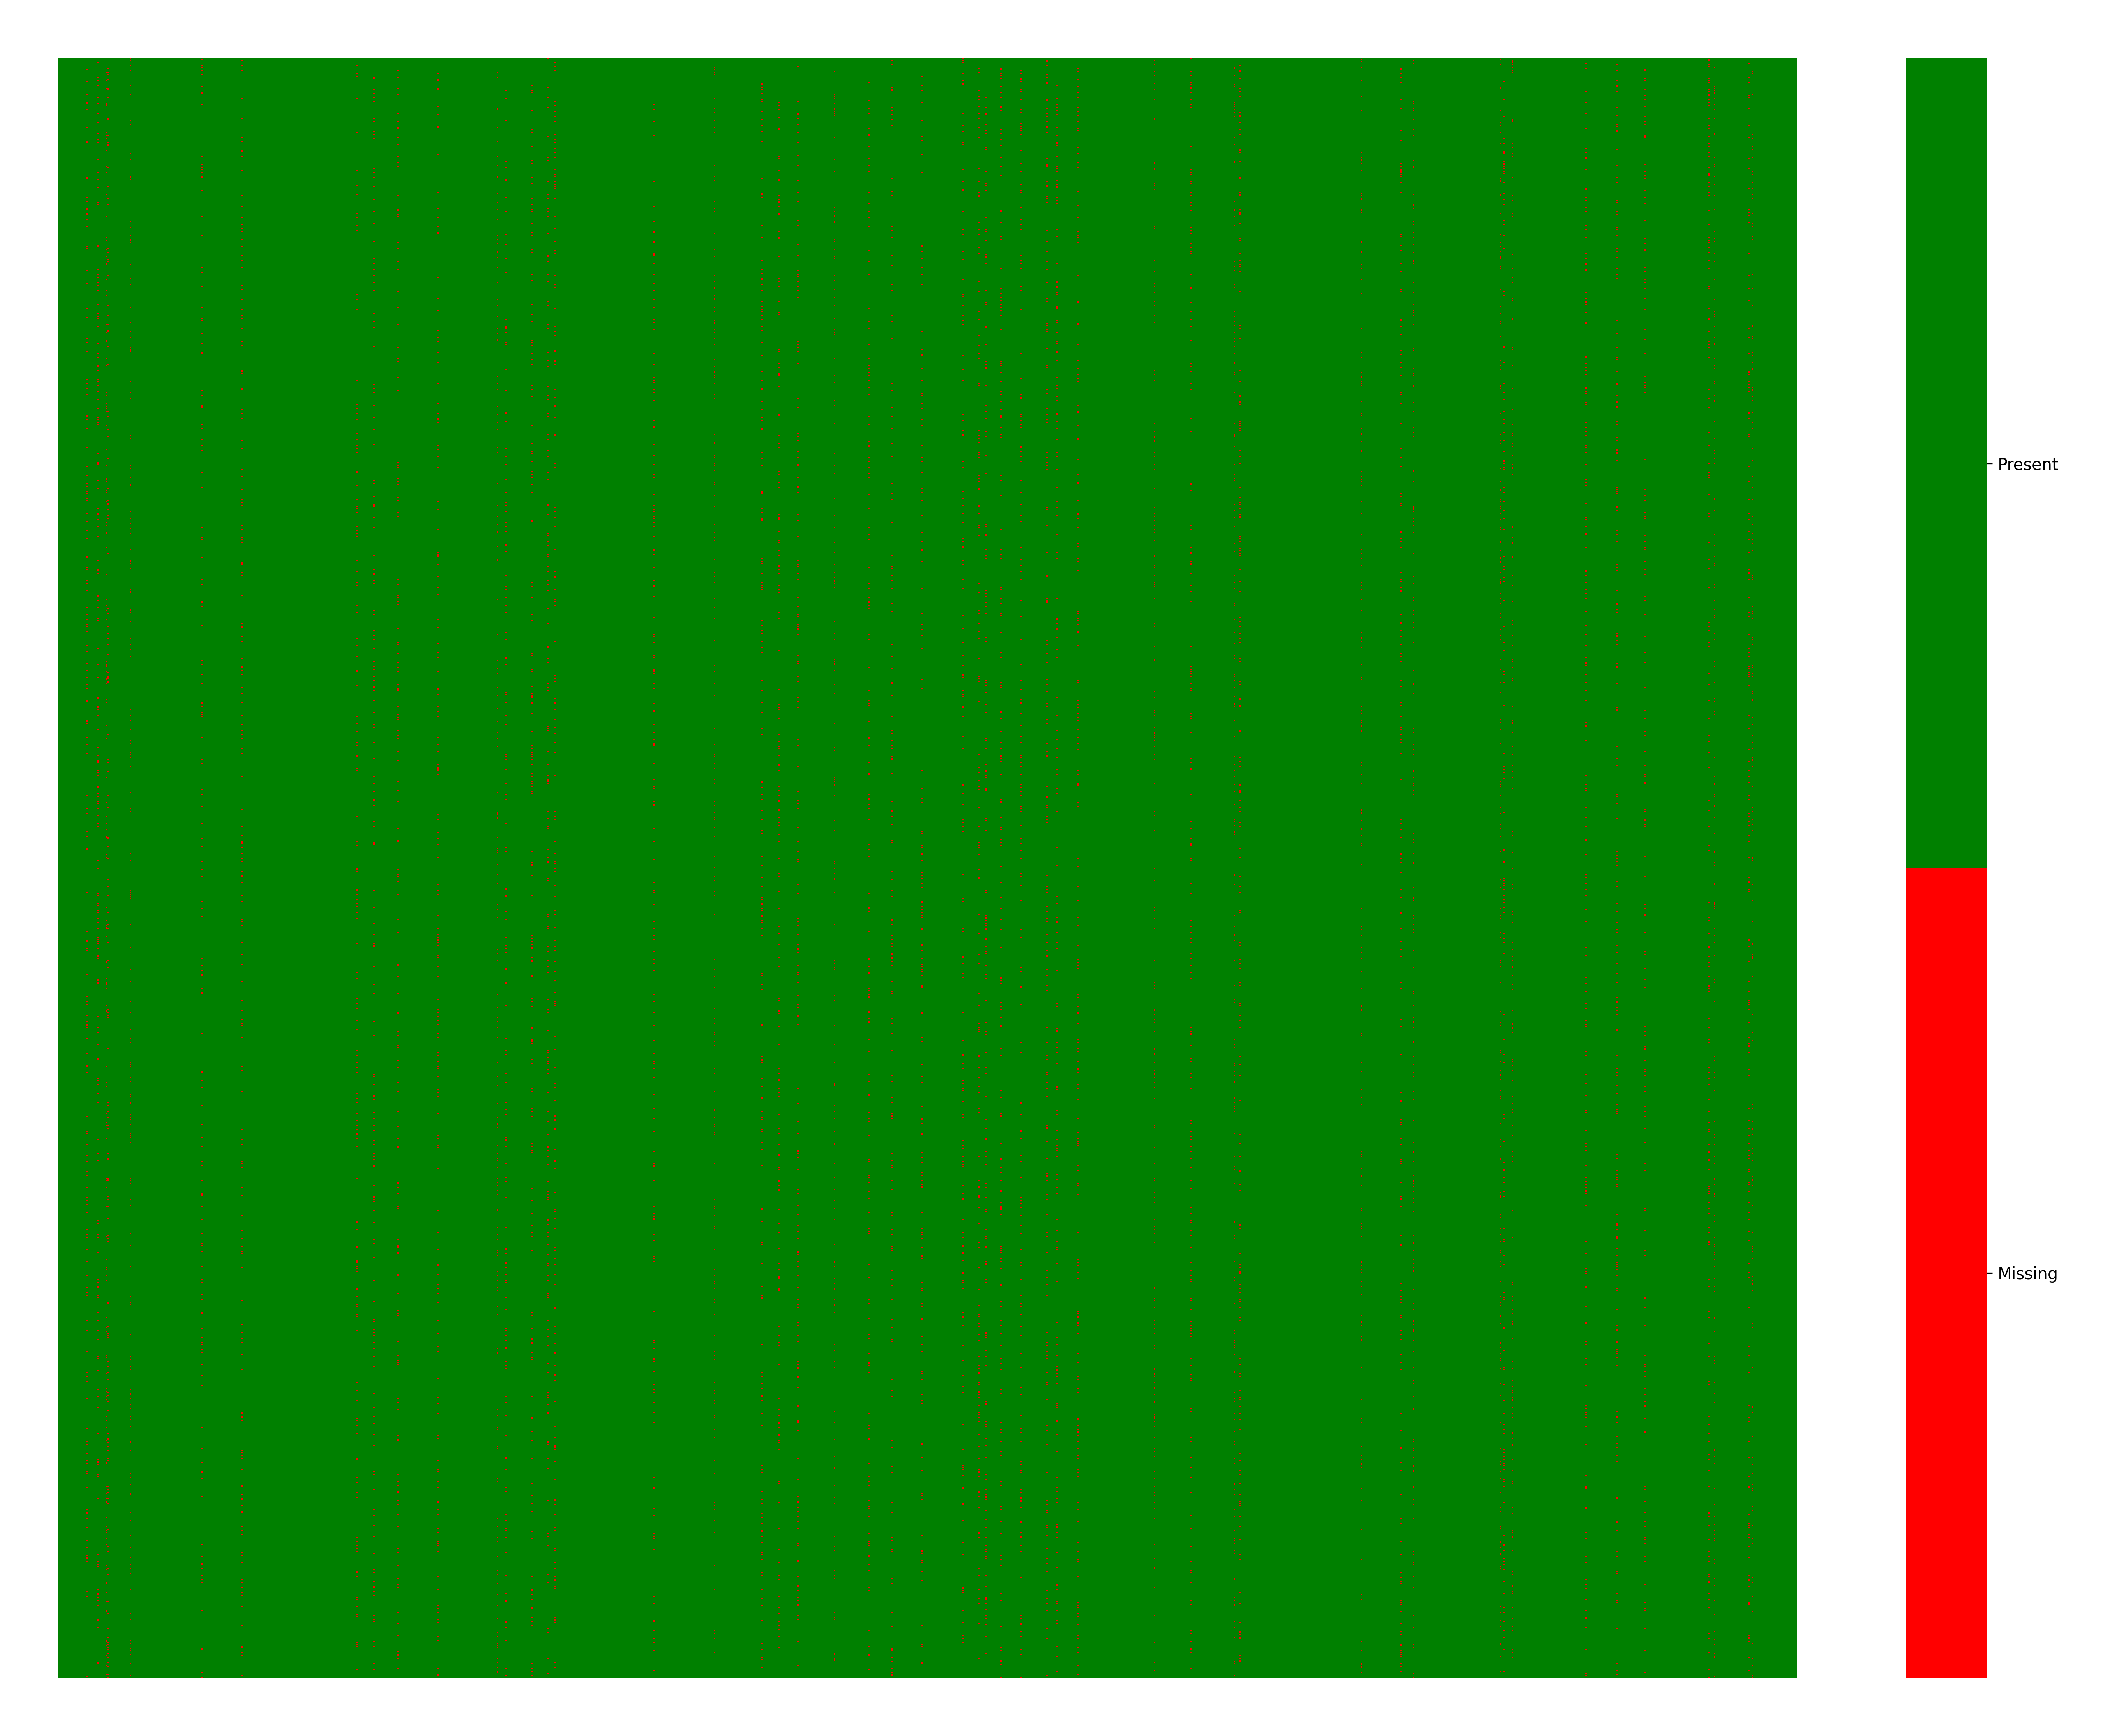
\includegraphics[width=0.5\linewidth]{case1_heatmap_erased.png}
    \caption{Case 1 Input Dataset}
\end{figure}

As shown, the dataset presents a homogeneous distribution of missing values. After applying v0.4, the structure of the data appears to be preserved, with no evident distortions (On the left, where originally the data had slightly more missing values, it is still well represented). In contrast, the heatmap for v0.3 displays many more missing values overall. This could indicate suboptimal handling of the number of values.

\begin{figure}[H]
    \centering
    \begin{subfigure}{0.45\textwidth}
        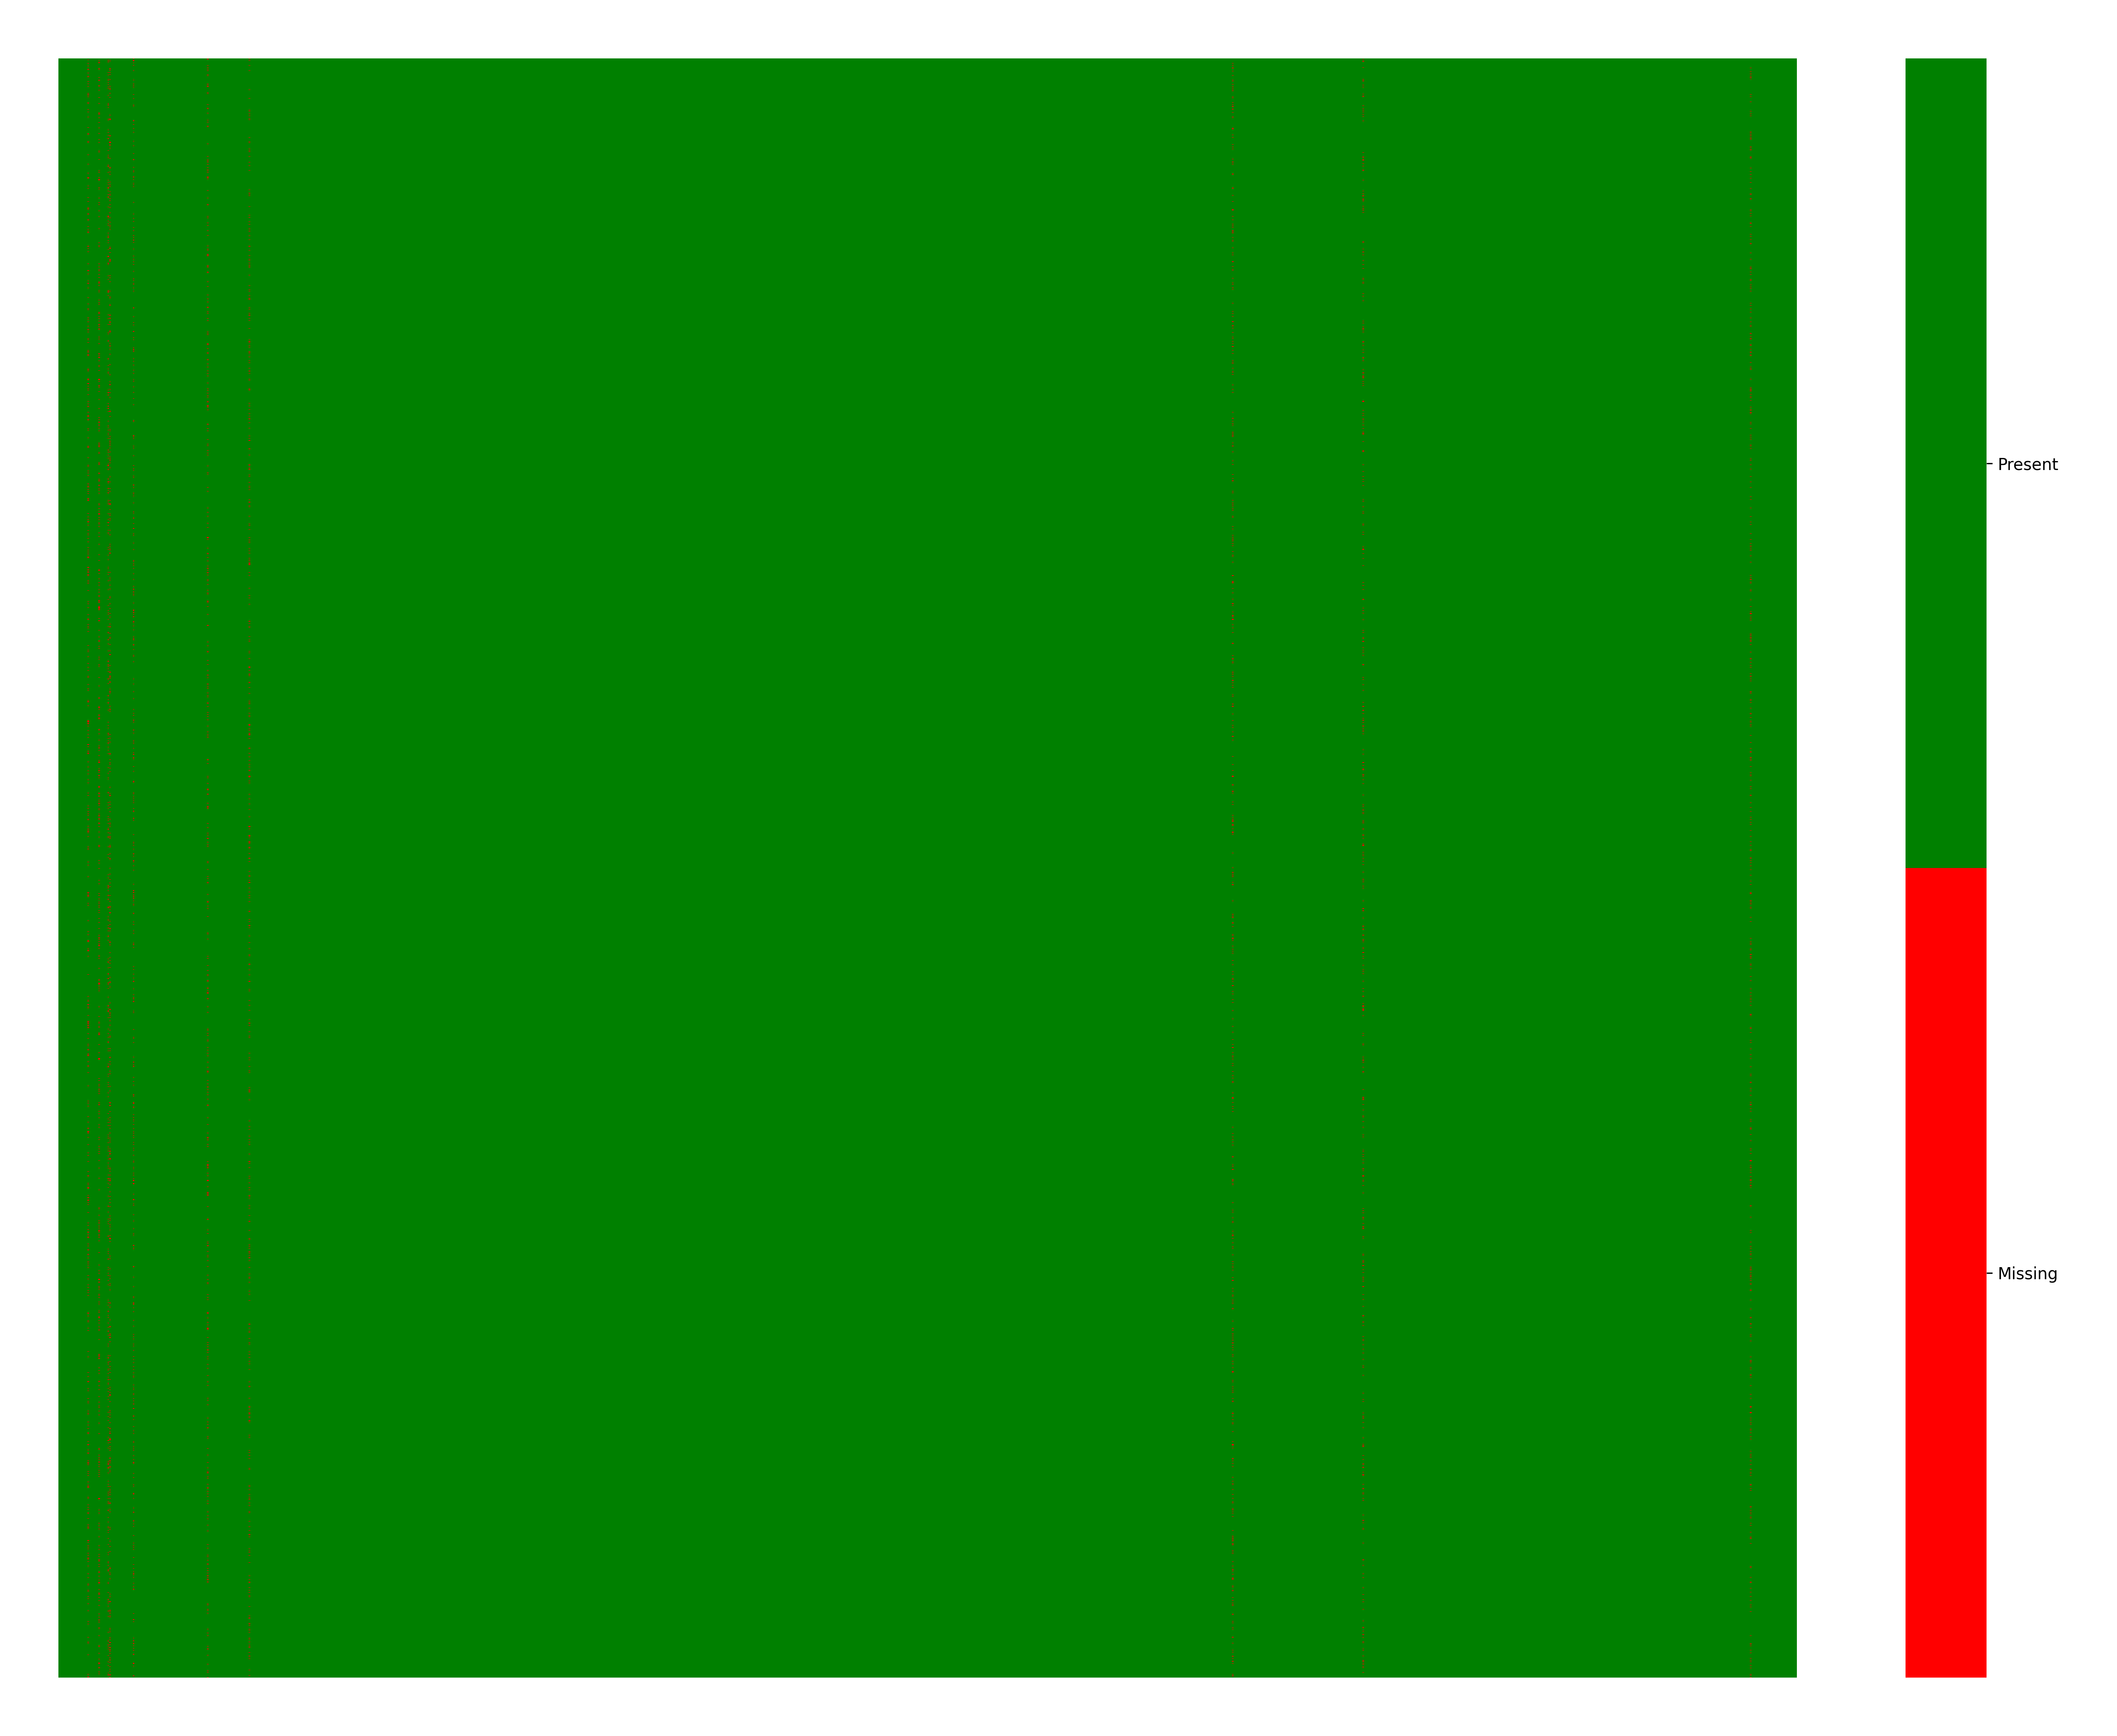
\includegraphics[width=\linewidth]{case1_v0.4_heatmap_cleaned.png}
        \caption{v0.4 (Best)}
    \end{subfigure}
    \hfill
    \begin{subfigure}{0.45\textwidth}
        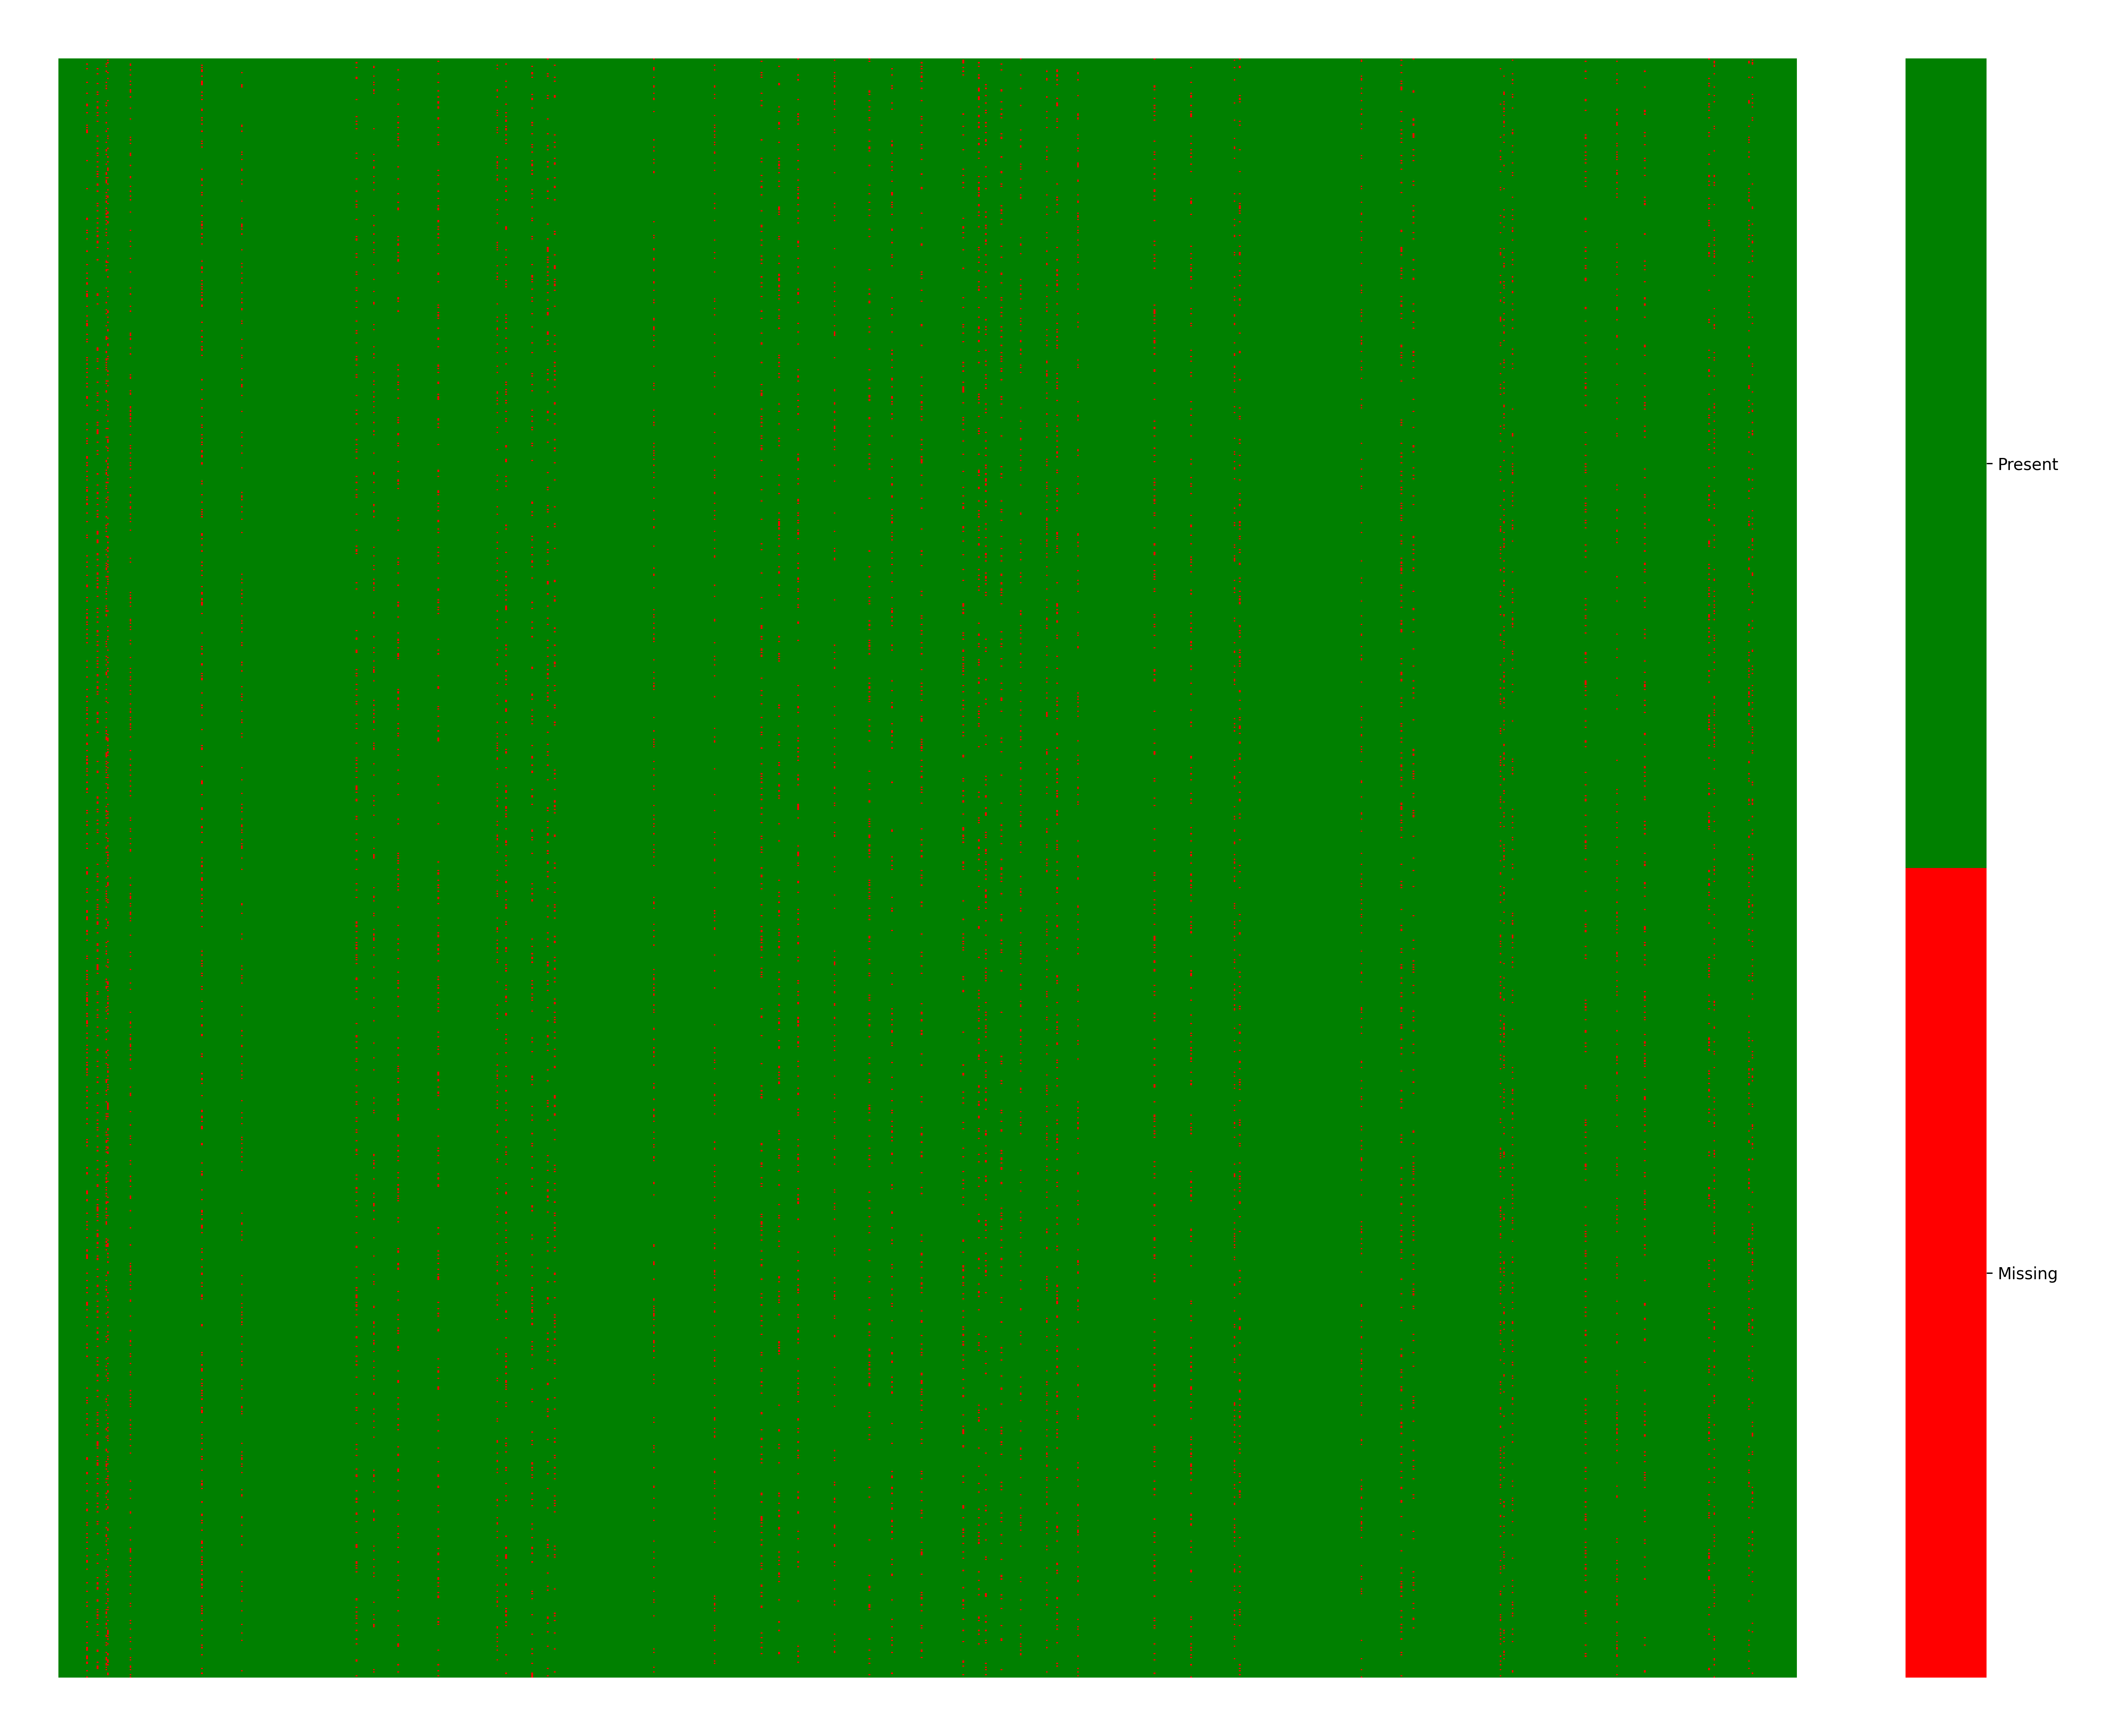
\includegraphics[width=\linewidth]{case1_v0.3_heatmap_cleaned.png}
        \caption{v0.3 (Worst)}
    \end{subfigure}
    \caption{Case 1 cleaned datasets comparison}
\end{figure}

\subsubsection{Case 2: MCAR – 25\%}

\textbf{Score Table:}

\begin{table}[H]
\centering
\caption{Scores by algorithm, Case 2}
\label{tab:score_algorithms_case2_new}
\begin{tabular}{|c|c|c|c|c|c|c|c|c|}
\hline
Algorithm & v0.0 & v0.1 & v0.2 & v0.3 & v0.4 & v0.5 & BnB & Average \\
\hline
Score & 54.9 & 53.6 & 50.5 & 63.1 & 85.1 & 85.1 & 52.0 & \textbf{56.04} \\
\hline
\end{tabular}
\end{table}

\textbf{Observations}\\
The highest-performing algorithms are v0.4 and v0.5, each with a health score of 85.1. This is also reflected in the Missing Value Reduction (27.6/30) and Constraint Adherence (40/40) components. The lowest score comes from v0.2 (50.5), due to a very low Missing Value Reduction score (9.0/30). The total performance gap between the best and worst scores is 34.6 points, indicating a significant difference in effectiveness. Notably, despite v0.0 being the simplest of the algorithms, it still achieves a surprisingly high ranking among the scores.

\textbf{Heatmaps}\\
We begin by inspecting the input dataset to verify that the missingness follows a uniform MCAR pattern.

\begin{figure}[H]
    \centering
    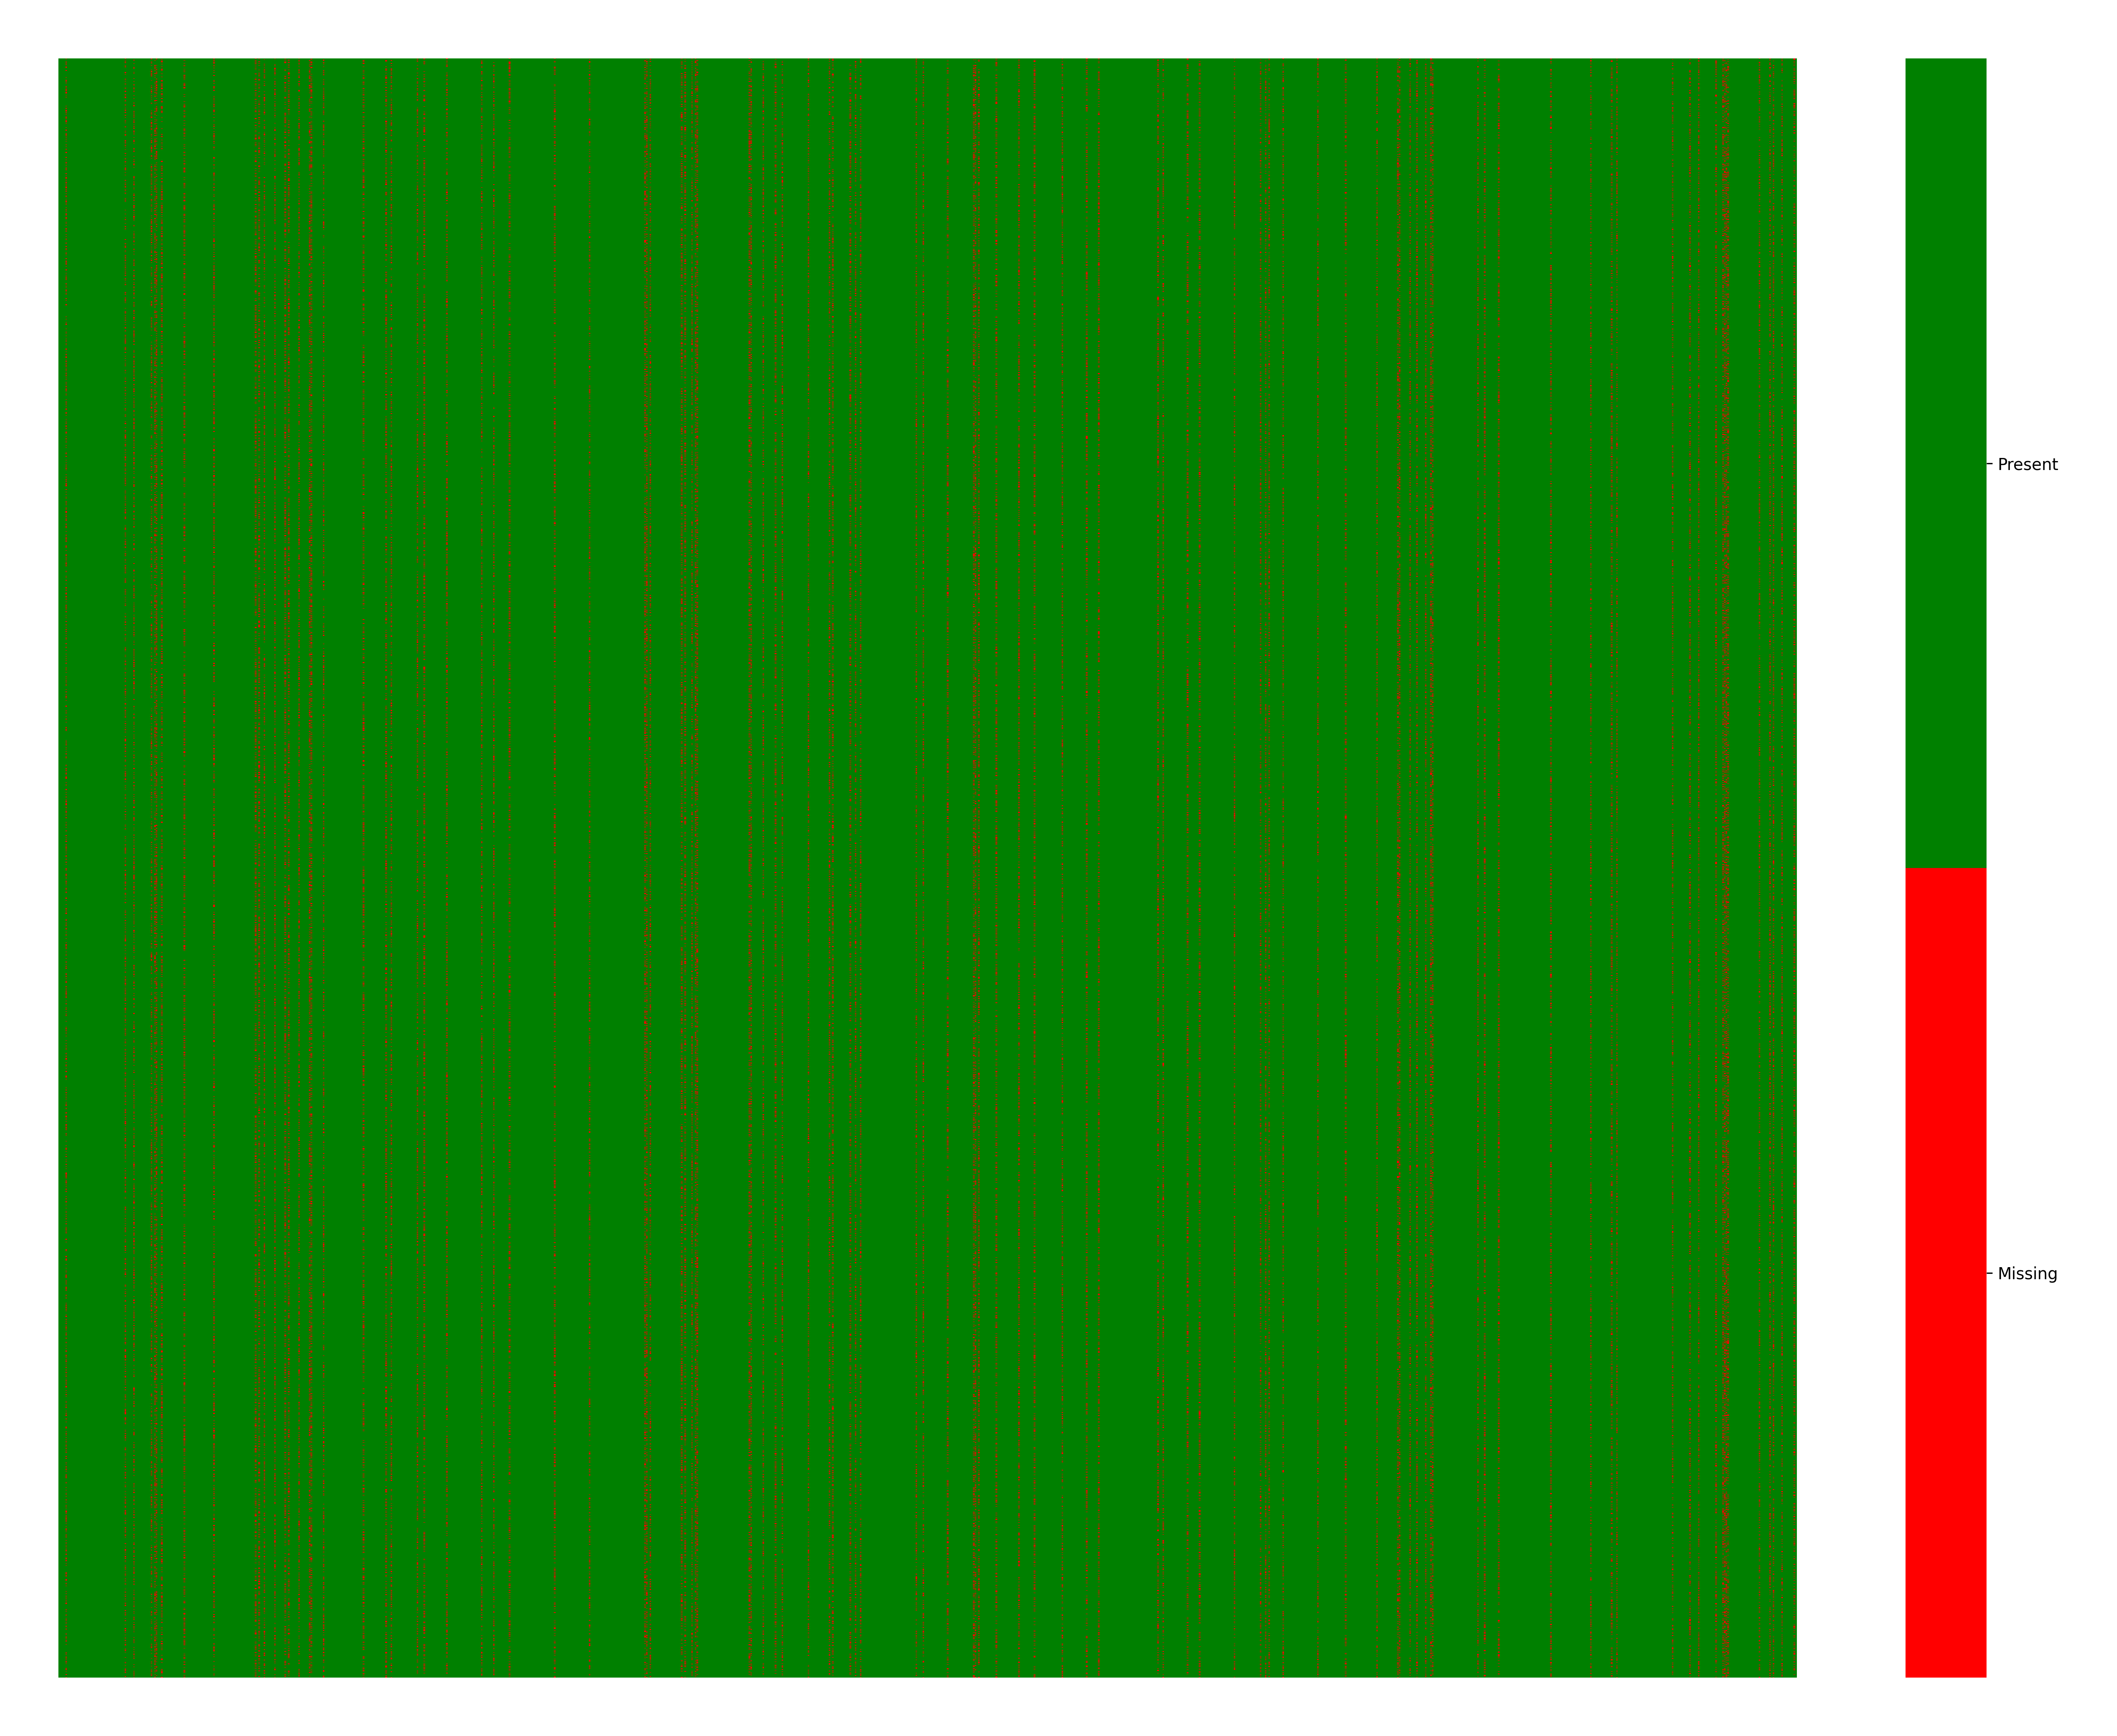
\includegraphics[width=0.5\linewidth]{case2_heatmap_erased.png}
    \caption{Case 2 Input Dataset}
\end{figure}

After applying v0.4 and v0.5, the overall matrix density is well preserved. We can clearly observe a significant reduction in missing values, which corresponds to their high health scores. In contrast, the heatmap for v0.2 shows considerably more missing values. The dataset appears visibly incomplete, highlighting its inefficiency.

\begin{figure}[H]
    \centering
    \begin{subfigure}{0.45\textwidth}
        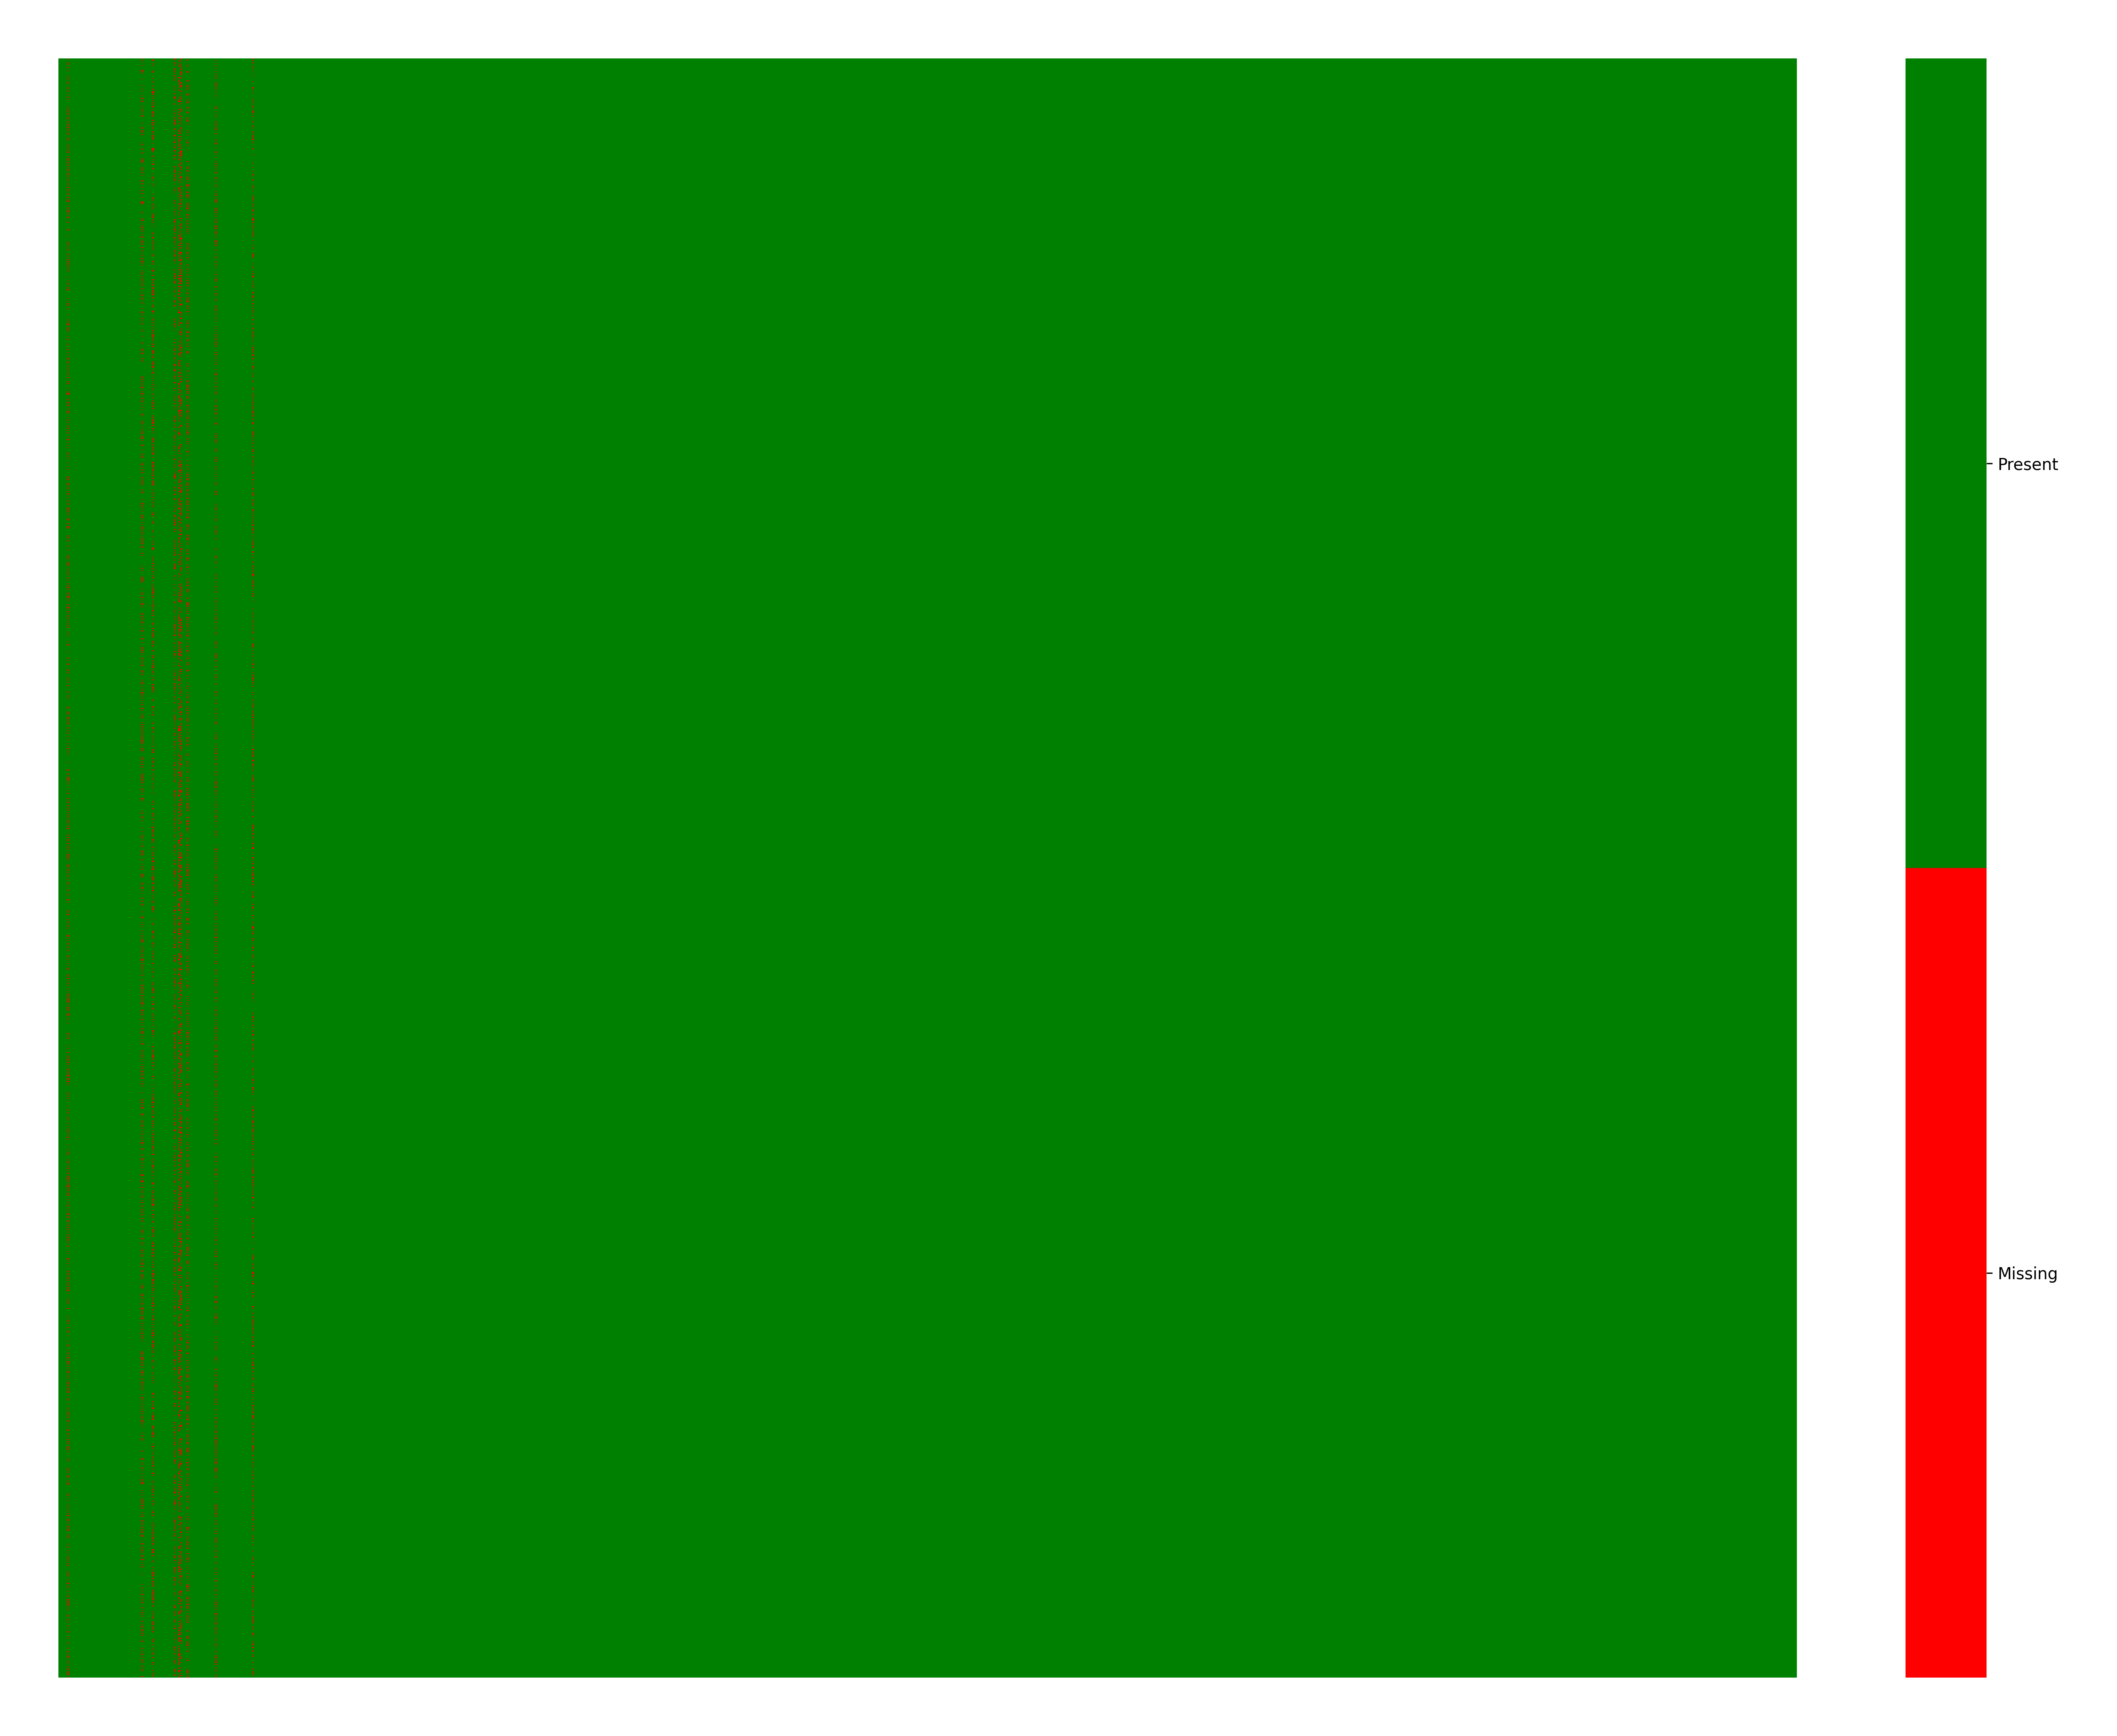
\includegraphics[width=\linewidth]{case2_v0.4_heatmap_cleaned.png}
        \caption{v0.4 (Best)}
    \end{subfigure}
    \hfill
    \begin{subfigure}{0.45\textwidth}
        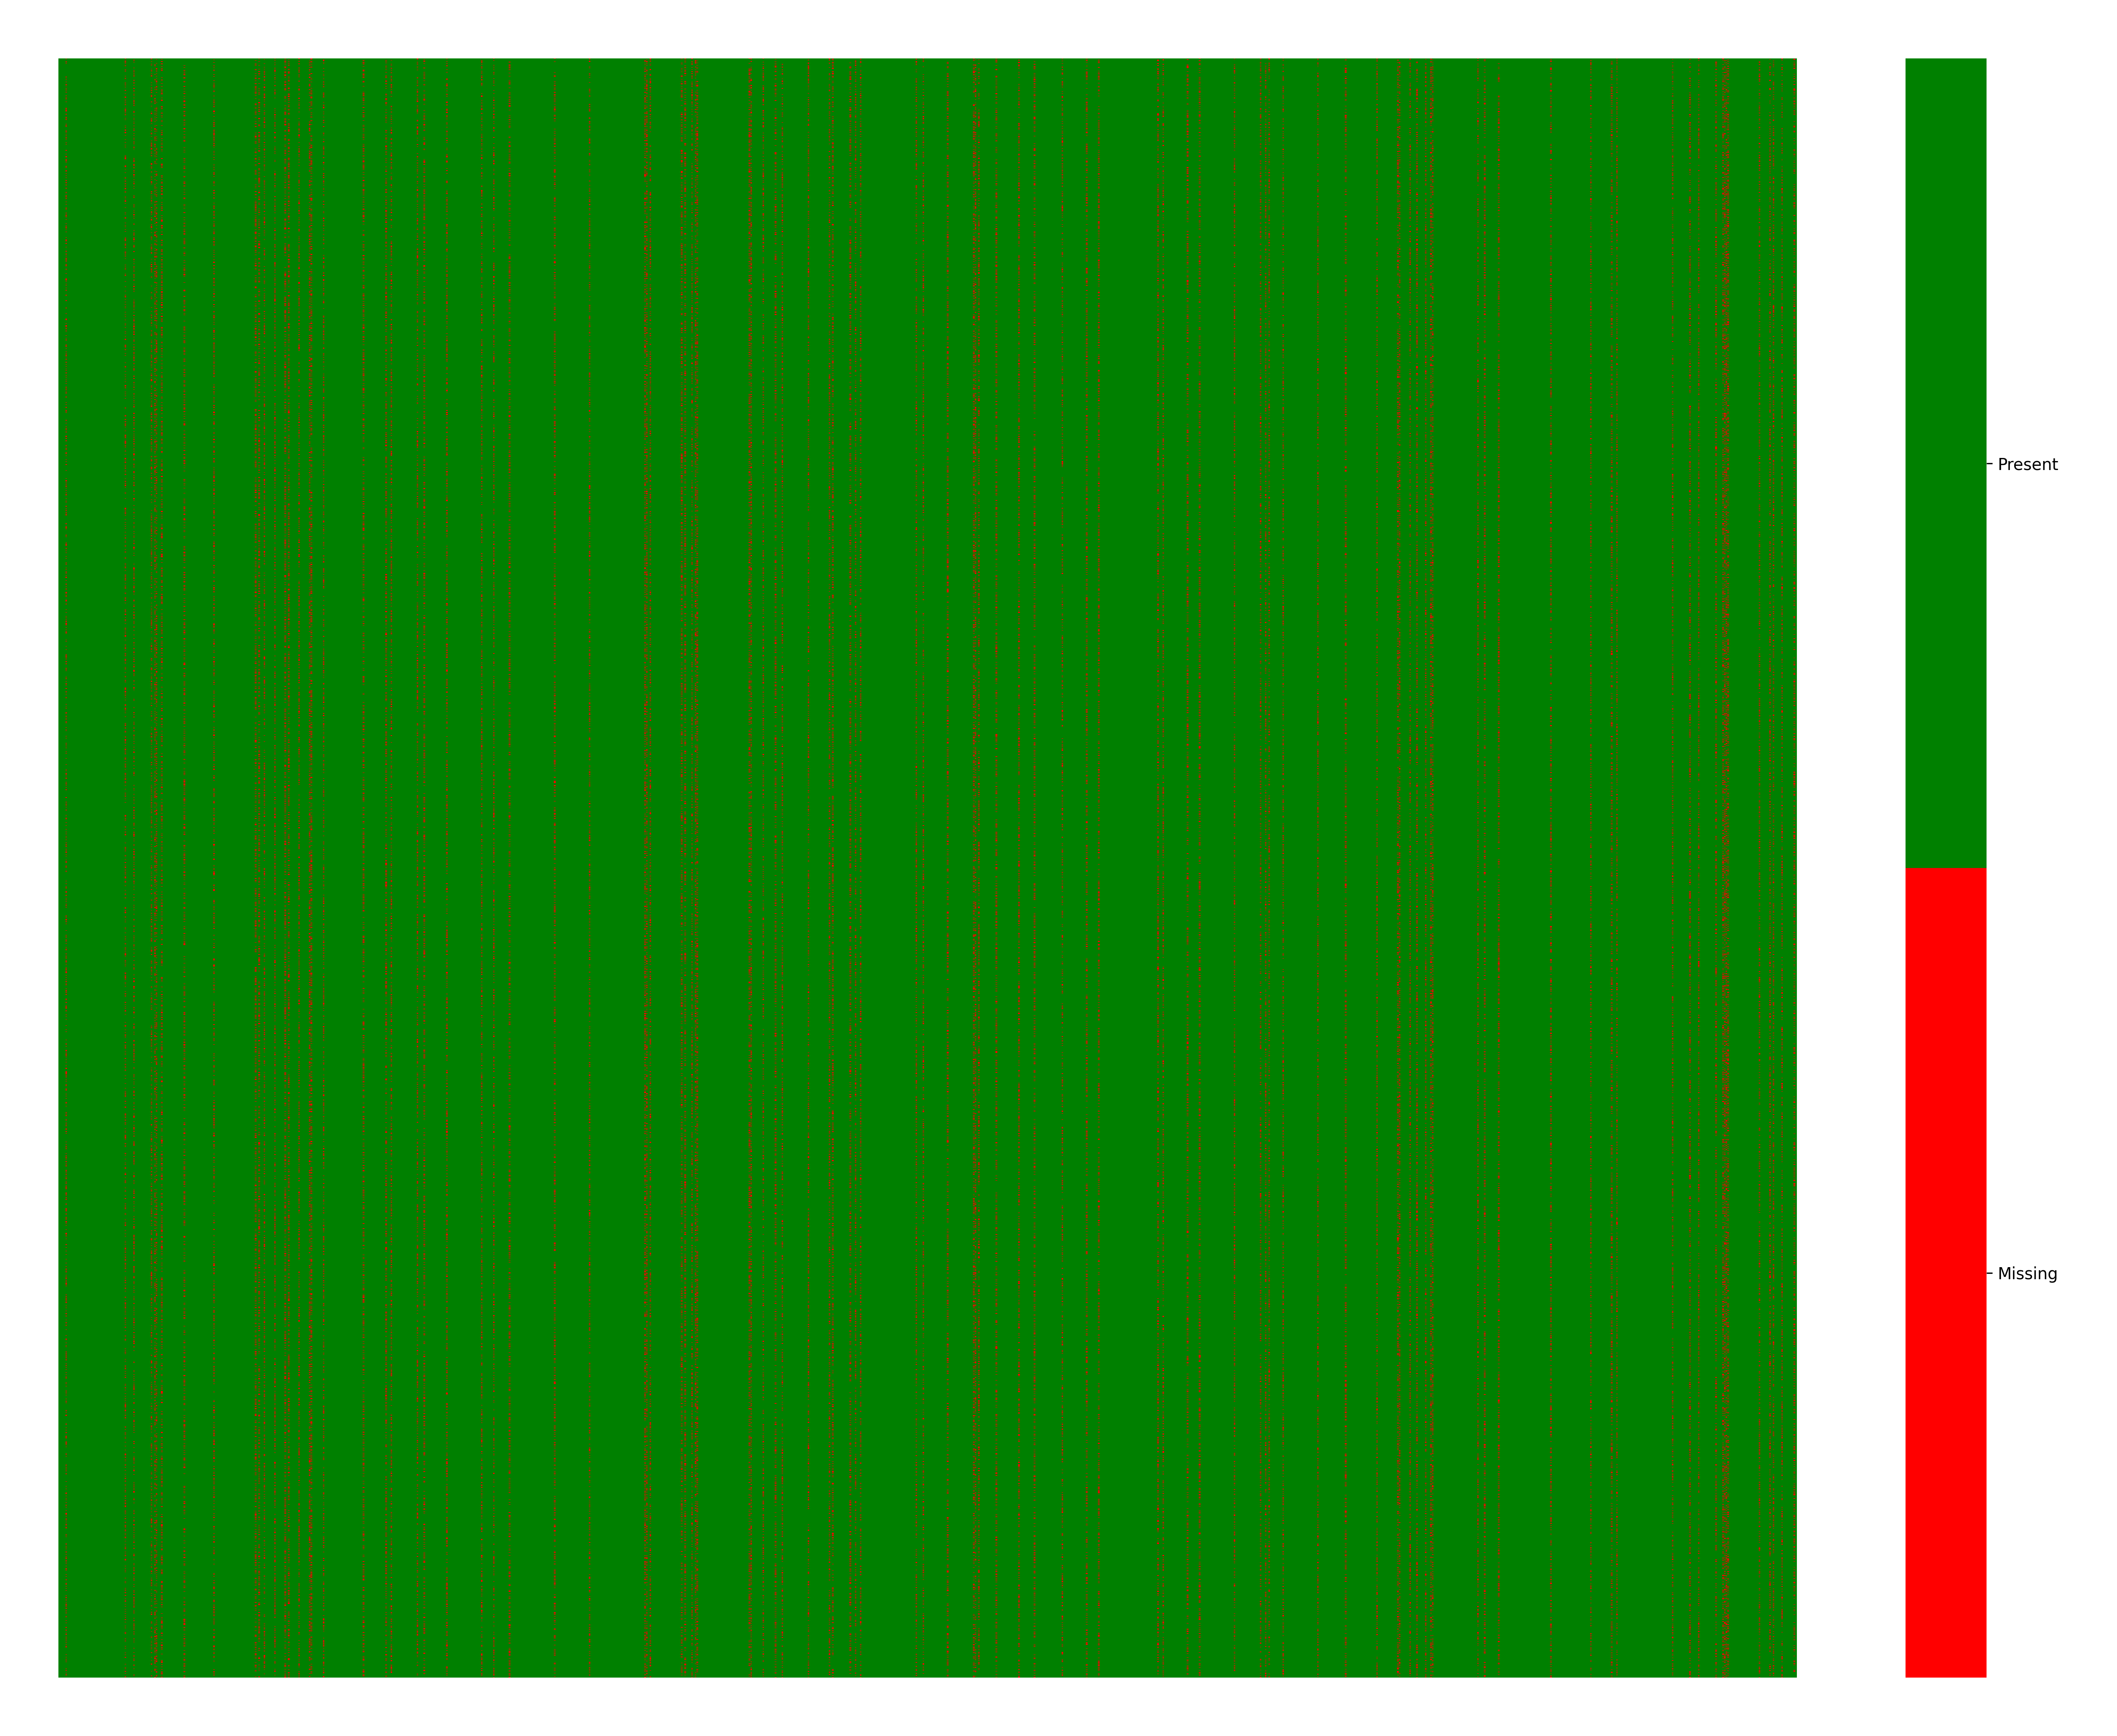
\includegraphics[width=\linewidth]{case2_v0.2_heatmap_cleaned.png}
        \caption{v0.2 (Worst)}
    \end{subfigure}
    \caption{Case 2 cleaned datasets comparison}
\end{figure}

\subsubsection{Case 3: MAR – Dependency on Three Reference Columns}

\textbf{Score Table:}

\begin{table}[H]
\centering
\caption{Scores by algorithm, Case 3}
\label{tab:score_algorithms_case3_new}
\begin{tabular}{|c|c|c|c|c|c|c|c|c|}
\hline
Algorithm & v0.0 & v0.1 & v0.2 & v0.3 & v0.4 & v0.5 & BnB & Average \\
\hline
Score & 69.6 & 60.0 & 61.7 & 52.2 & 60.0 & 60.0 & 60.0 & \textbf{60.5} \\
\hline
\end{tabular}
\end{table}

\textbf{Observations}\\
Surprisingly, v0.0 is the top performing algorithm, achieving a score of 69.6. It has solid results across all health components. The lowest score comes from v0.3 (52.2), with notably low adherence (32/40) and retention (17.5/20). The total performance gap between the best and worst scores is 17.4 points, showing lower variance compared to other cases. 

\textbf{Heatmaps}\\
We begin by inspecting the input dataset to verify that the missingness pattern reflects a MAR process, where missing values are conditionally dependent on reference columns. As expected, missingness is concentrated in specific columns, confirming the intended structure.

\begin{figure}[H]
    \centering
    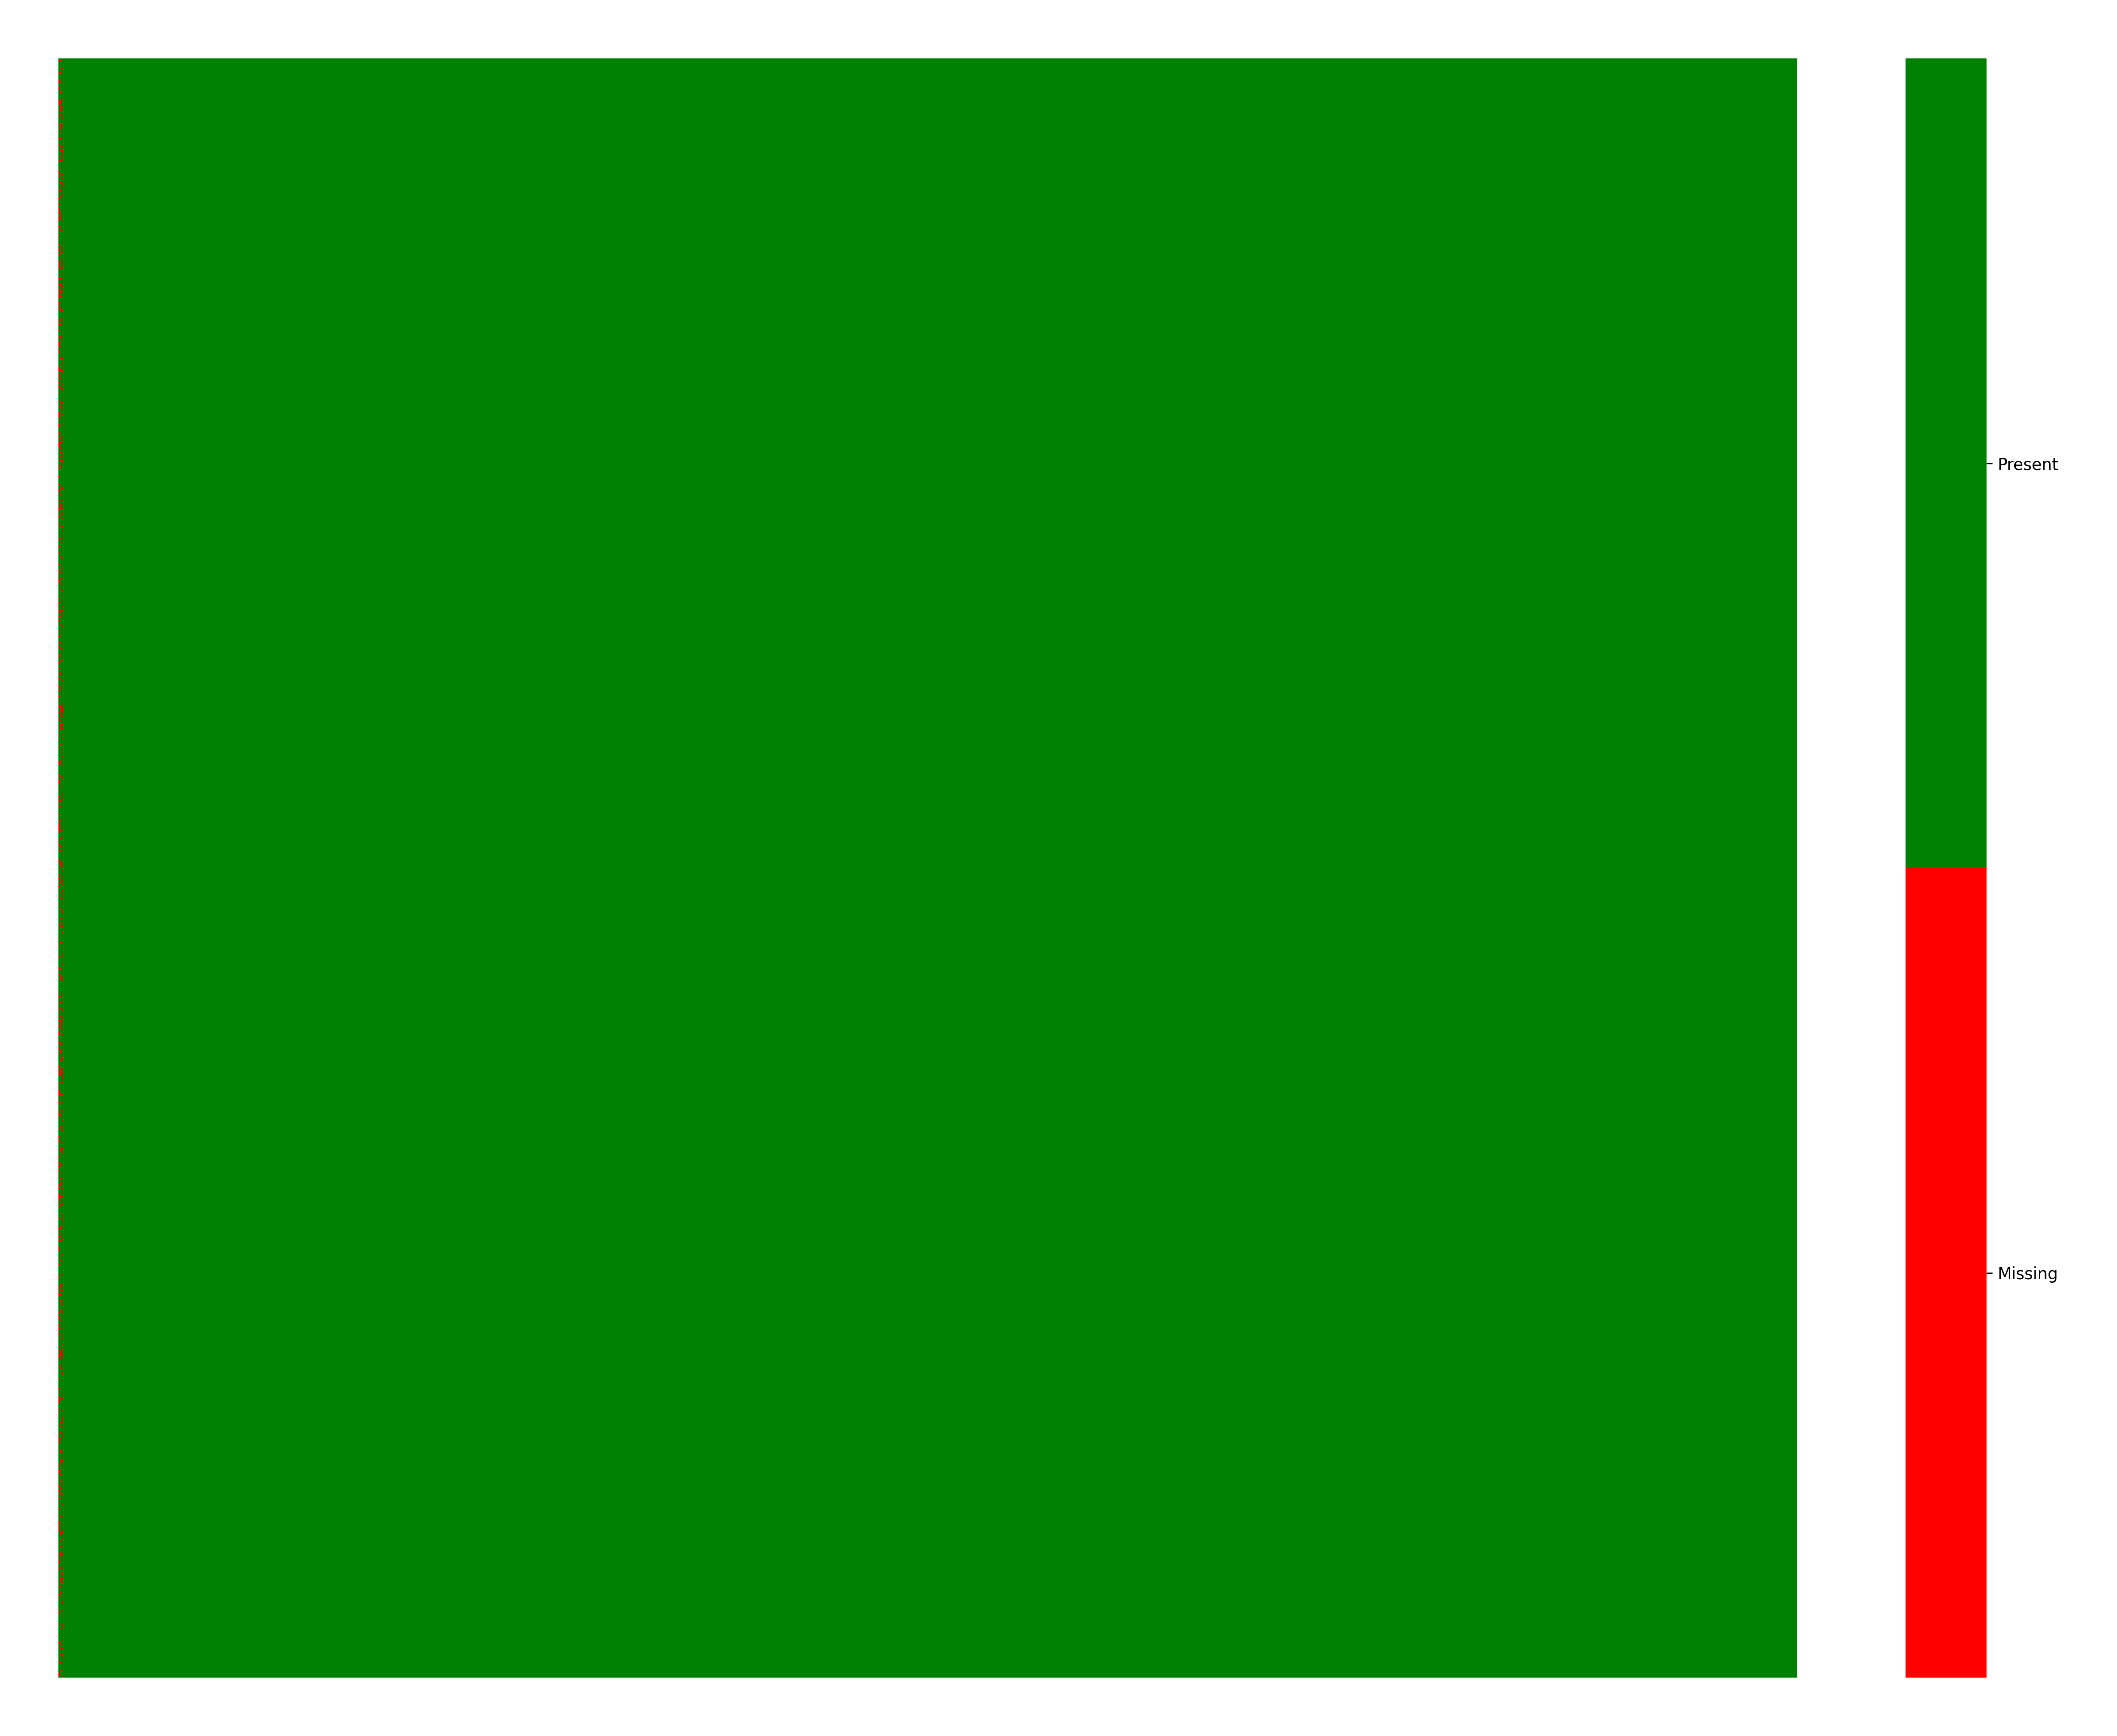
\includegraphics[width=0.5\linewidth]{case3_heatmap_erased.png}
    \caption{Case 3 Input Dataset}
\end{figure}

After applying v0.0, we can see good handling around the missing regions. We clearly observe a significant reduction in missing values while conserving internal structures. In contrast, the heatmap for v0.3 shows what could be classified as over-imputation, indicating poor handling of MAR dependencies.

\begin{figure}[H]
    \centering
    \begin{subfigure}{0.45\textwidth}
        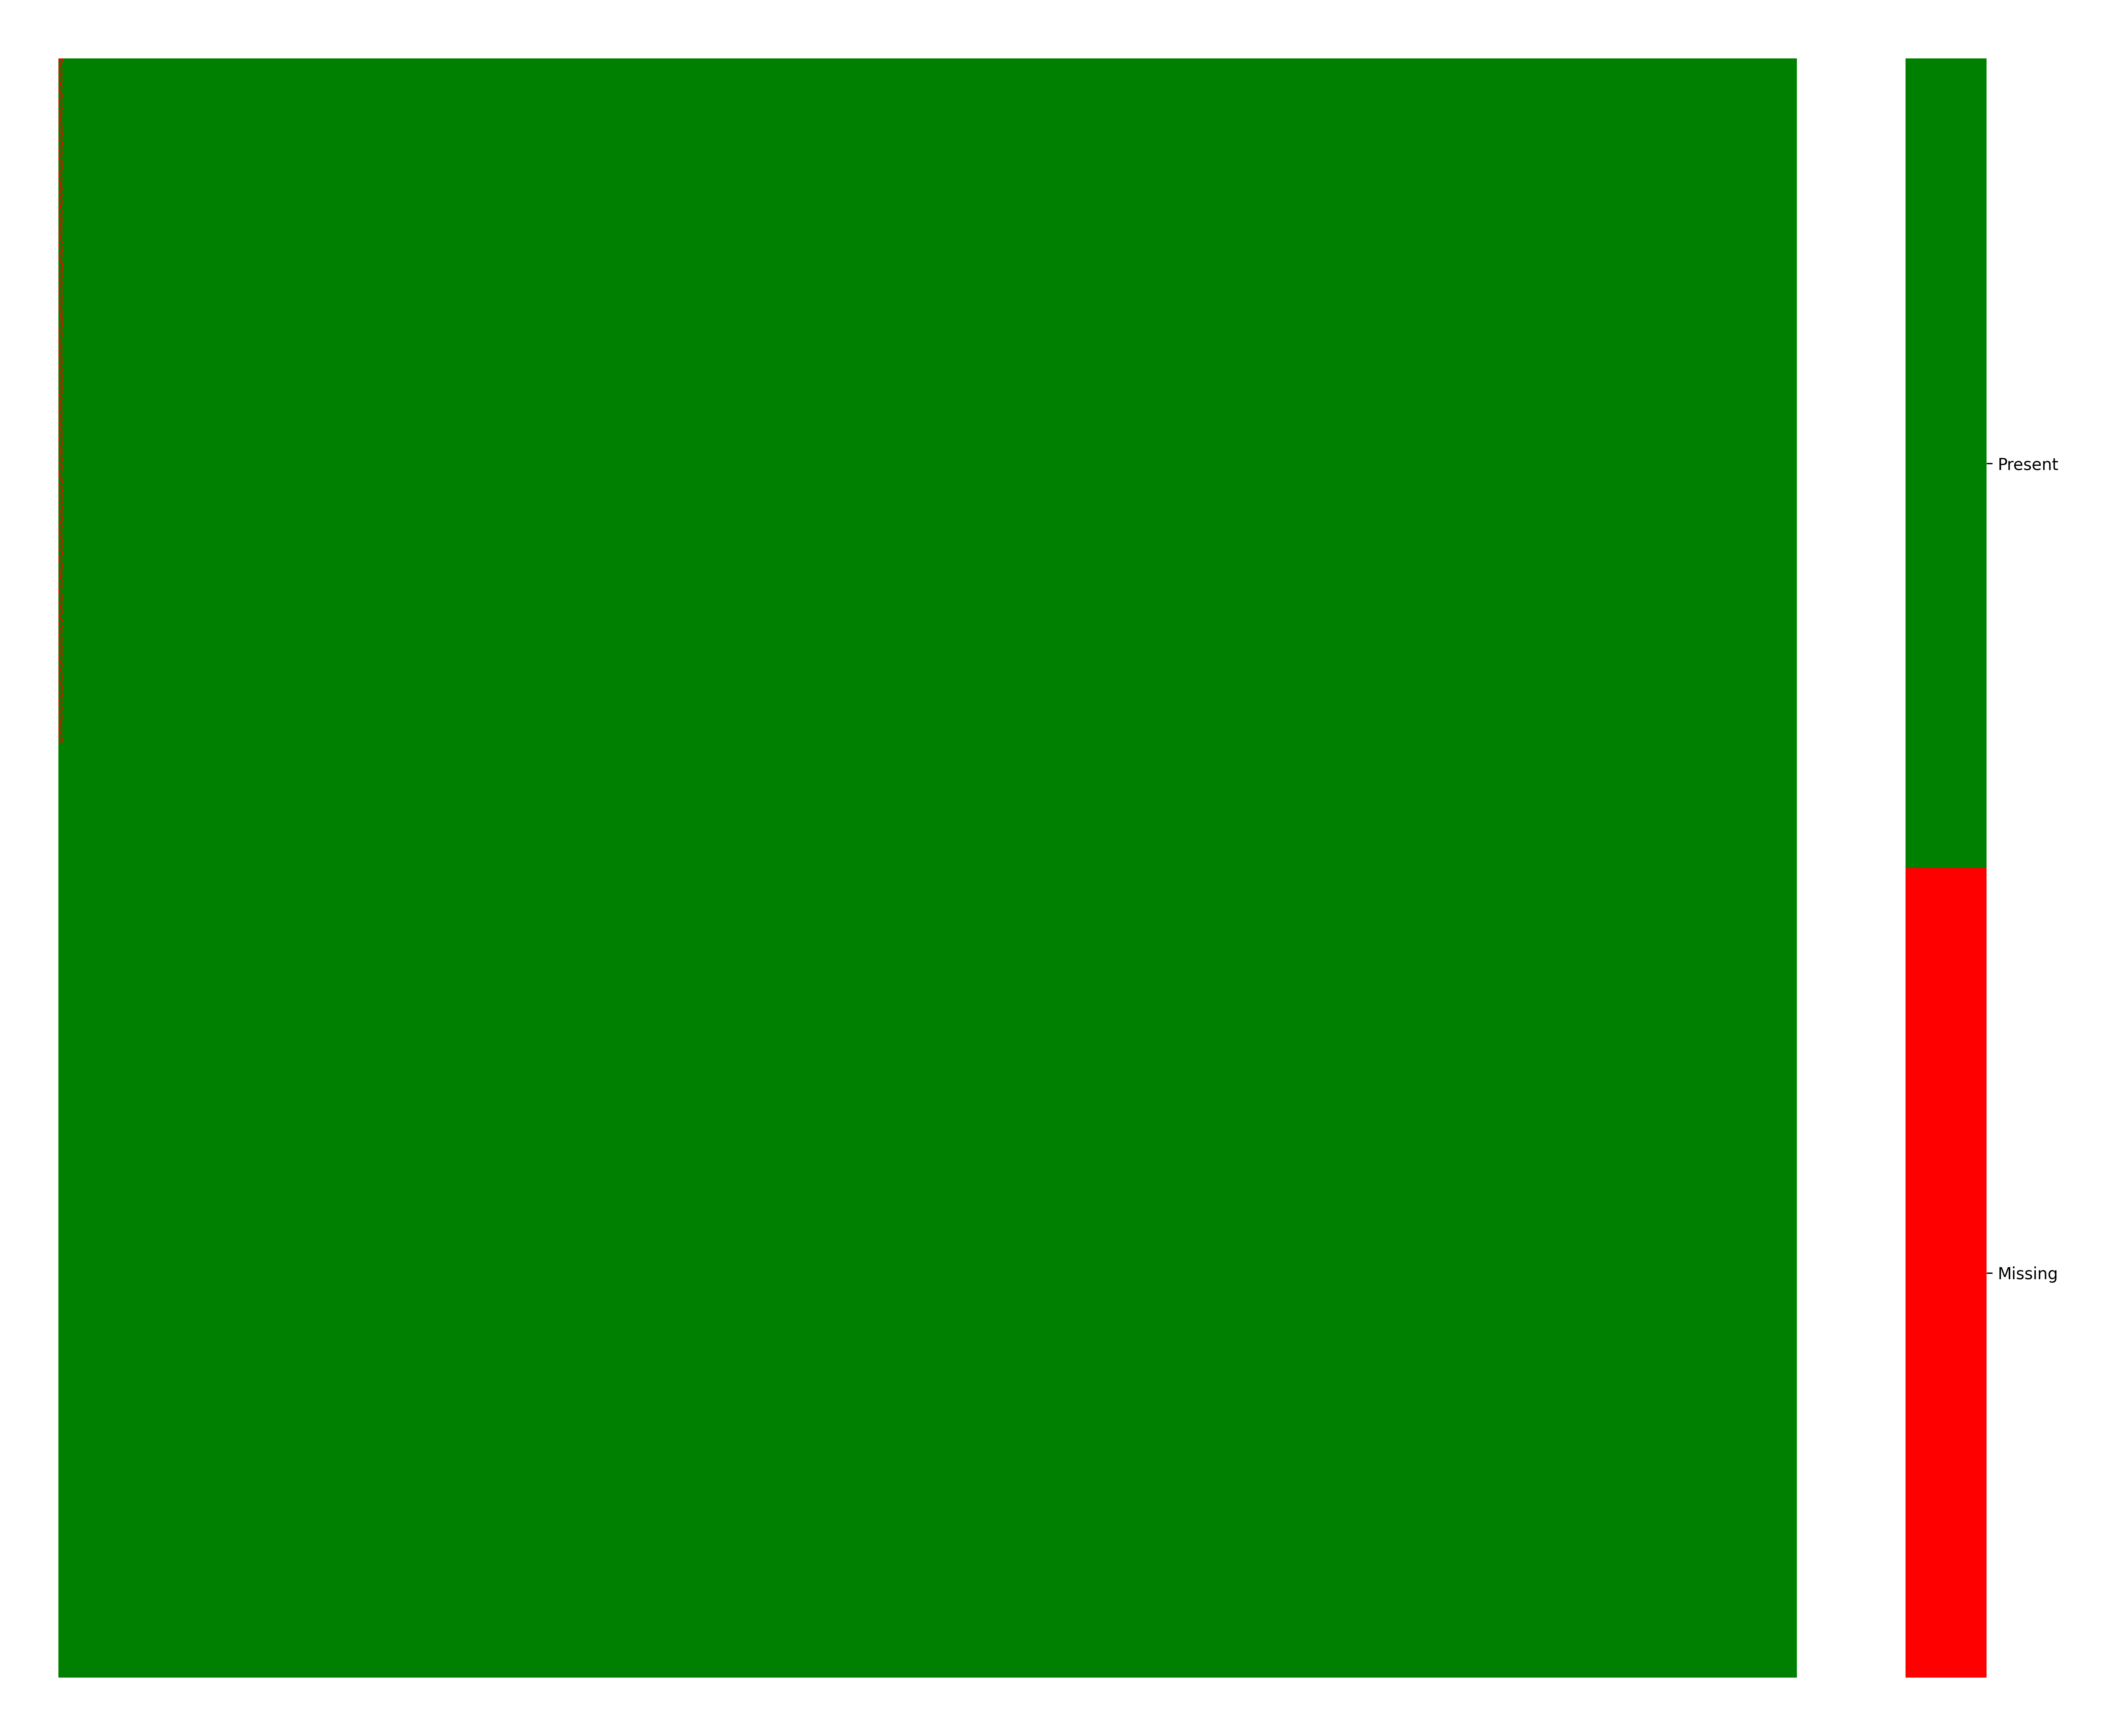
\includegraphics[width=\linewidth]{case3_v0.0_heatmap_cleaned.png}
        \caption{v0.0 (Best)}
    \end{subfigure}
    \hfill
    \begin{subfigure}{0.45\textwidth}
        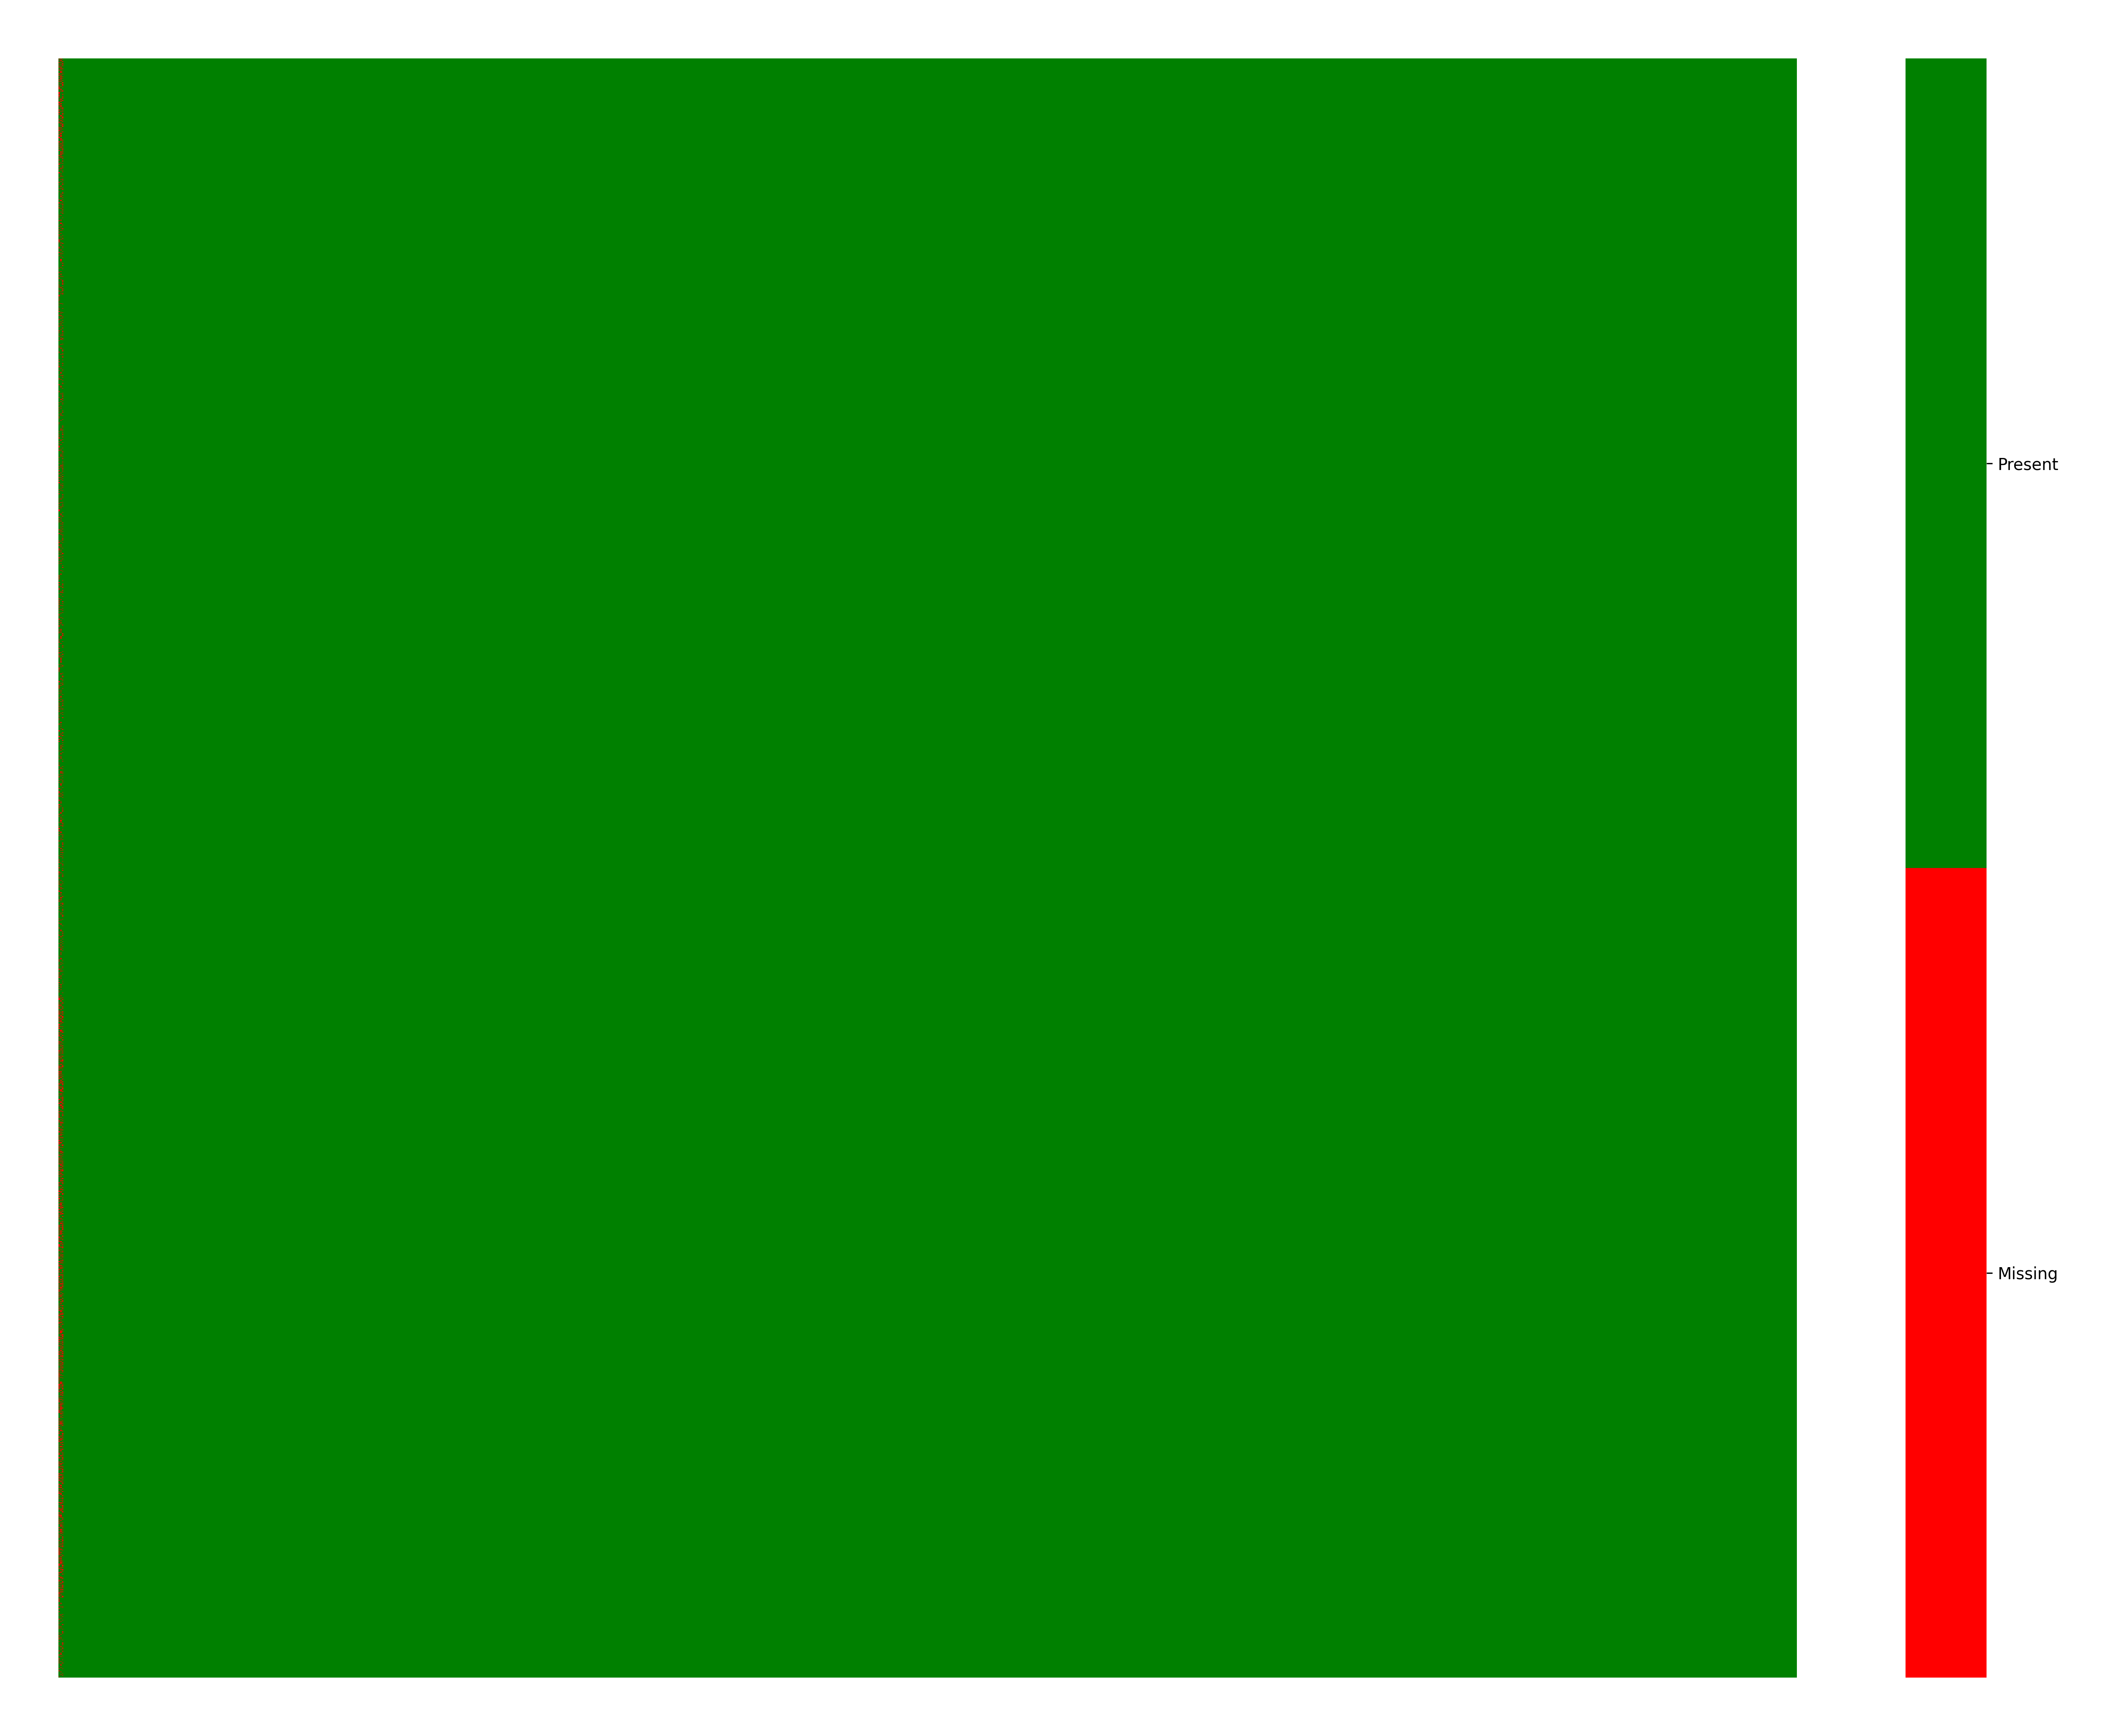
\includegraphics[width=\linewidth]{case3_v0.3_heatmap_cleaned.png}
        \caption{v0.3 (Worst)}
    \end{subfigure}
    \caption{Case 3 cleaned datasets comparison}
\end{figure}

\subsubsection{Case 4: MAR – Dependency on Five Reference Columns}

\textbf{Score Table:}

\begin{table}[H]
\centering
\caption{Scores by algorithm, Case 4}
\label{tab:score_algorithms_case4_new}
\begin{tabular}{|c|c|c|c|c|c|c|c|c|}
\hline
Algorithm & v0.0 & v0.1 & v0.2 & v0.3 & v0.4 & v0.5 & BnB & Average \\
\hline
Score & 64.9 & 62.7 & 64.4 & 52.6 & 60.7 & 60.7 & 70.0 & \textbf{62.29} \\
\hline
\end{tabular}
\end{table}

\textbf{Observations}\\
BnB outperforms all other algorithms with a score of 70.0. It has perfect results in constraint adherence, retention, and bonus. The lowest score comes from v0.3 (52.6), with notably low adherence (24/40) and retention (13.7/20). The performance gap between best and worst is 17.4 points, again showing low variance. 

\textbf{Heatmaps}\\
We begin by examining the input dataset to verify the MAR pattern, where missingness is conditioned on five specific reference columns. As seen below, the distribution is concentrated yet structurally coherent, as intended.

\begin{figure}[H]
    \centering
    
\includegraphics[width=0.5\linewidth]{case4_heatmap_erased.png}
    \caption{Case 4 Input Dataset}
\end{figure}

After applying BnB, we see excellent preservation of column relationships. We clearly observe significant reduction in missing values while conserving MAR dependencies. In contrast, v0.3 shows what we again classify as over-imputation.

\begin{figure}[H]
    \centering
    \begin{subfigure}{0.45\textwidth}
        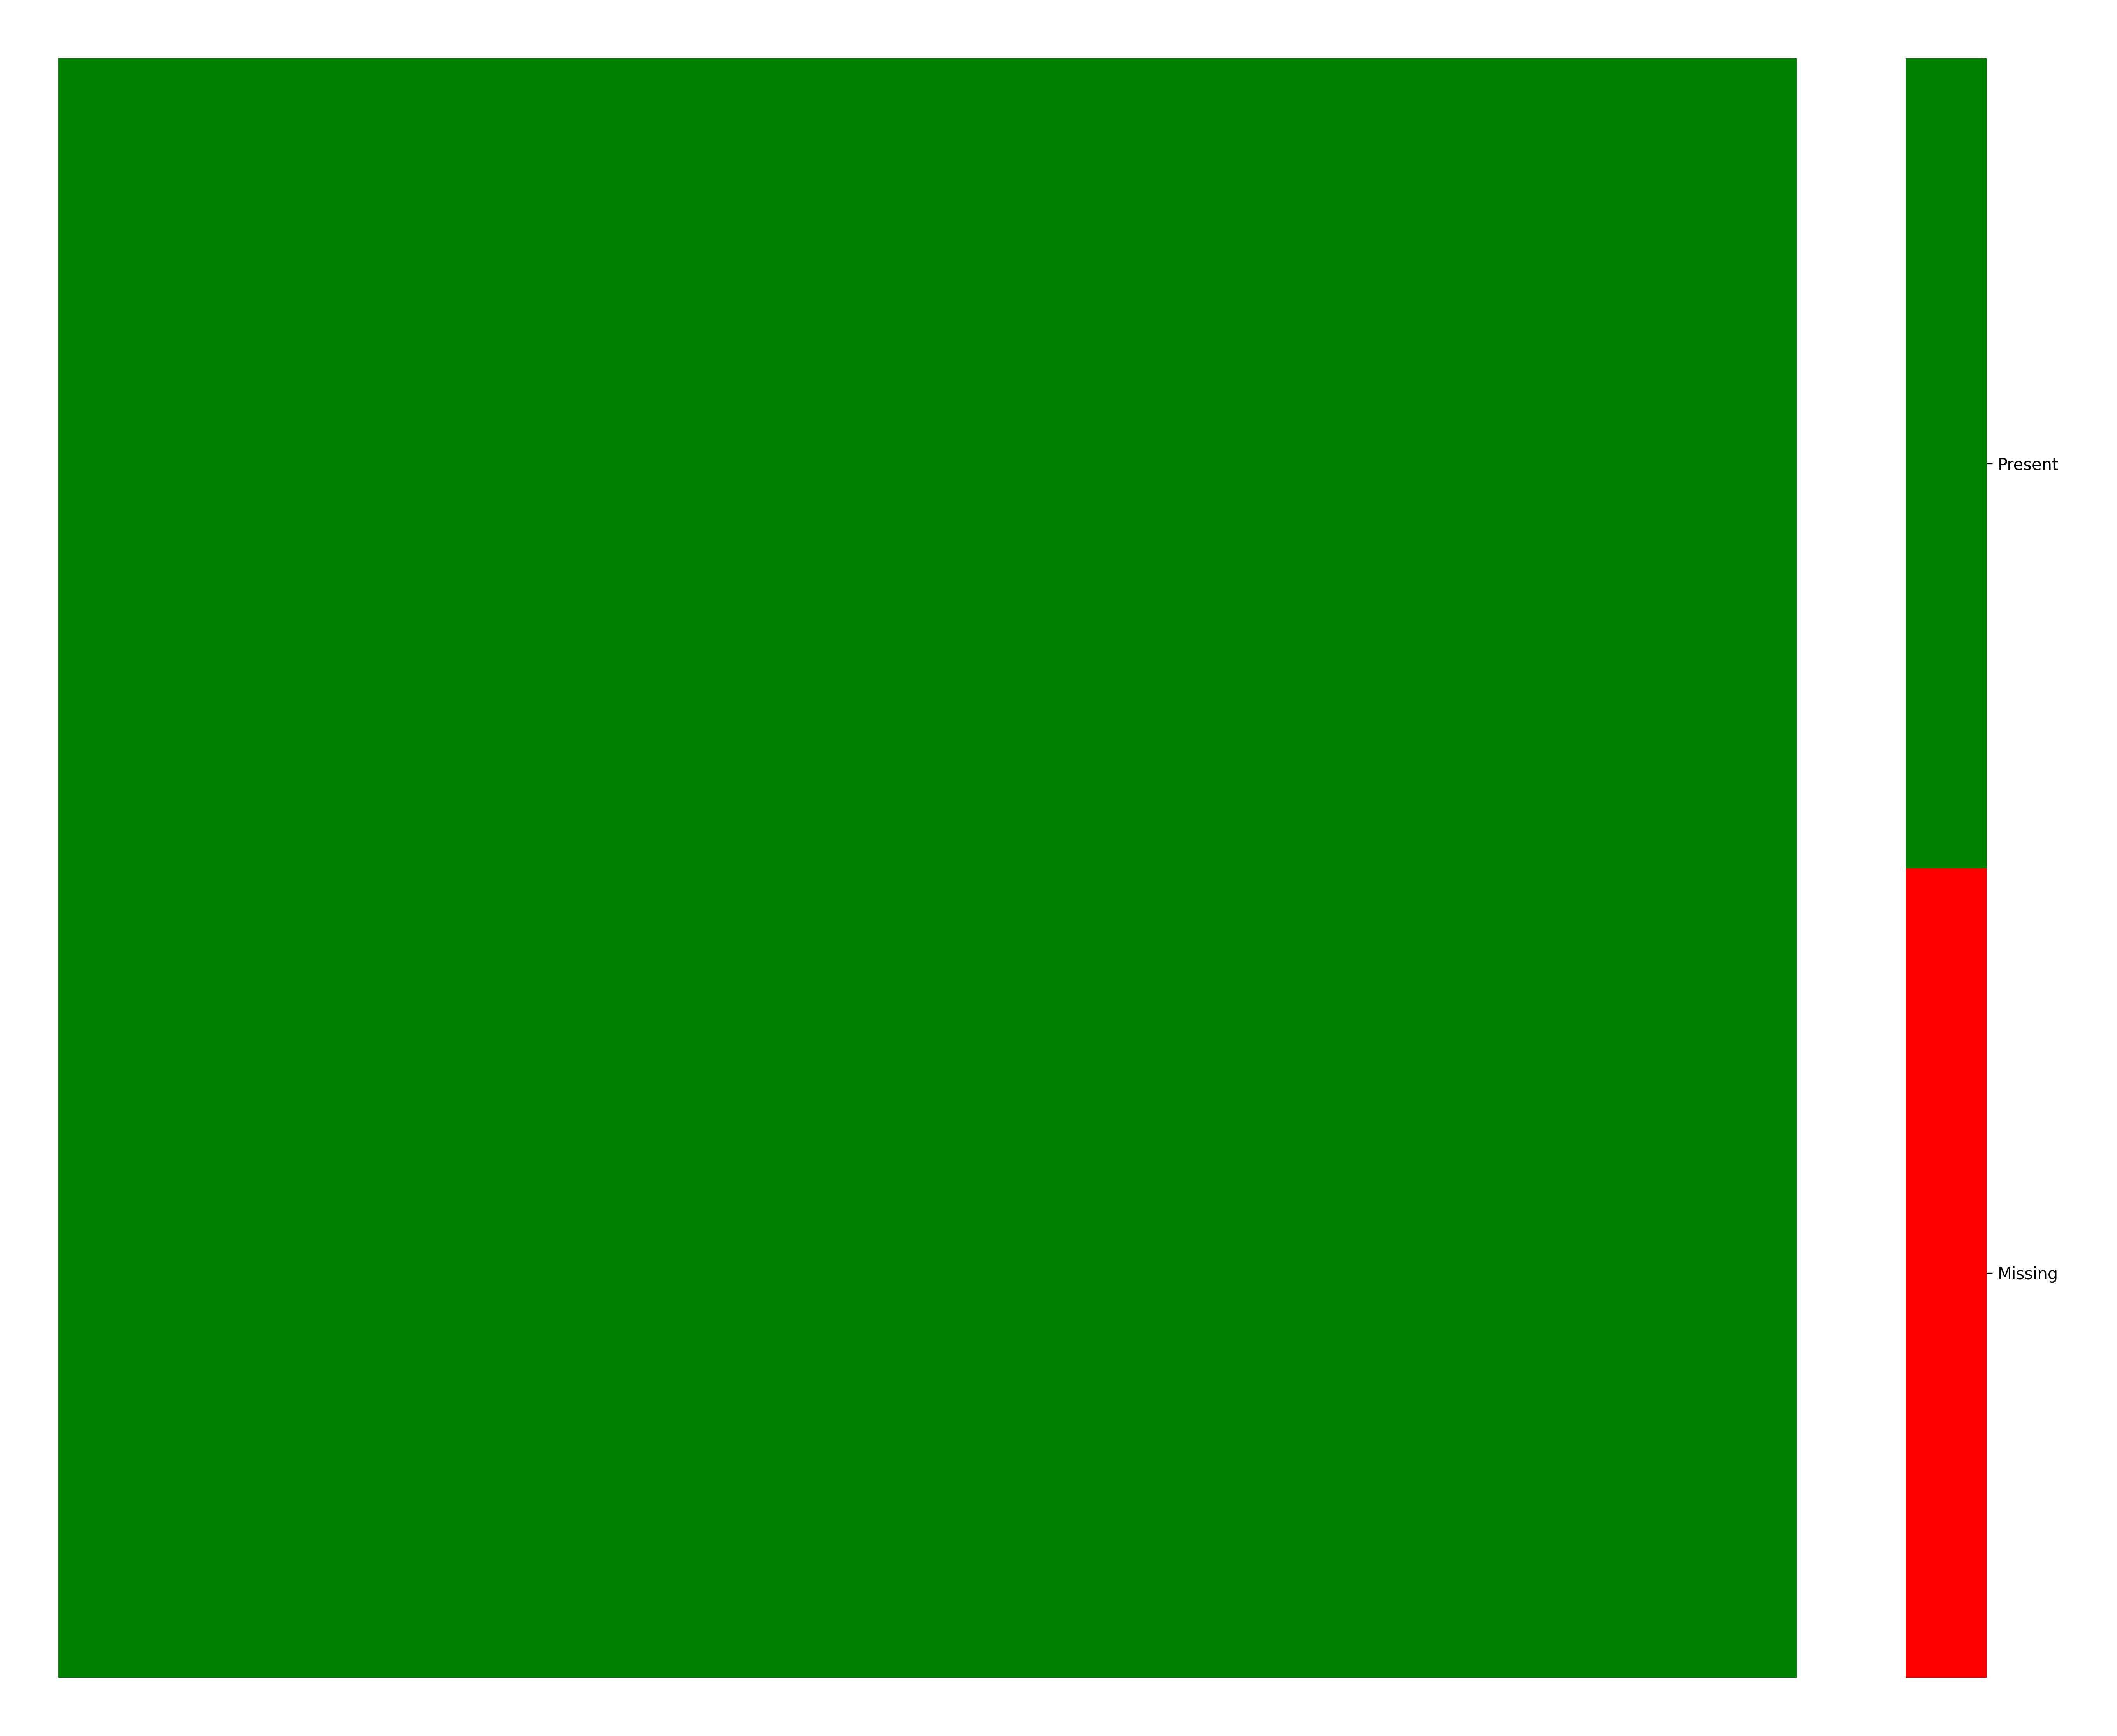
\includegraphics[width=\linewidth]{case4_bnb_heatmap_cleaned.png}
        \caption{BnB (Best)}
    \end{subfigure}
    \hfill
    \begin{subfigure}{0.45\textwidth}
        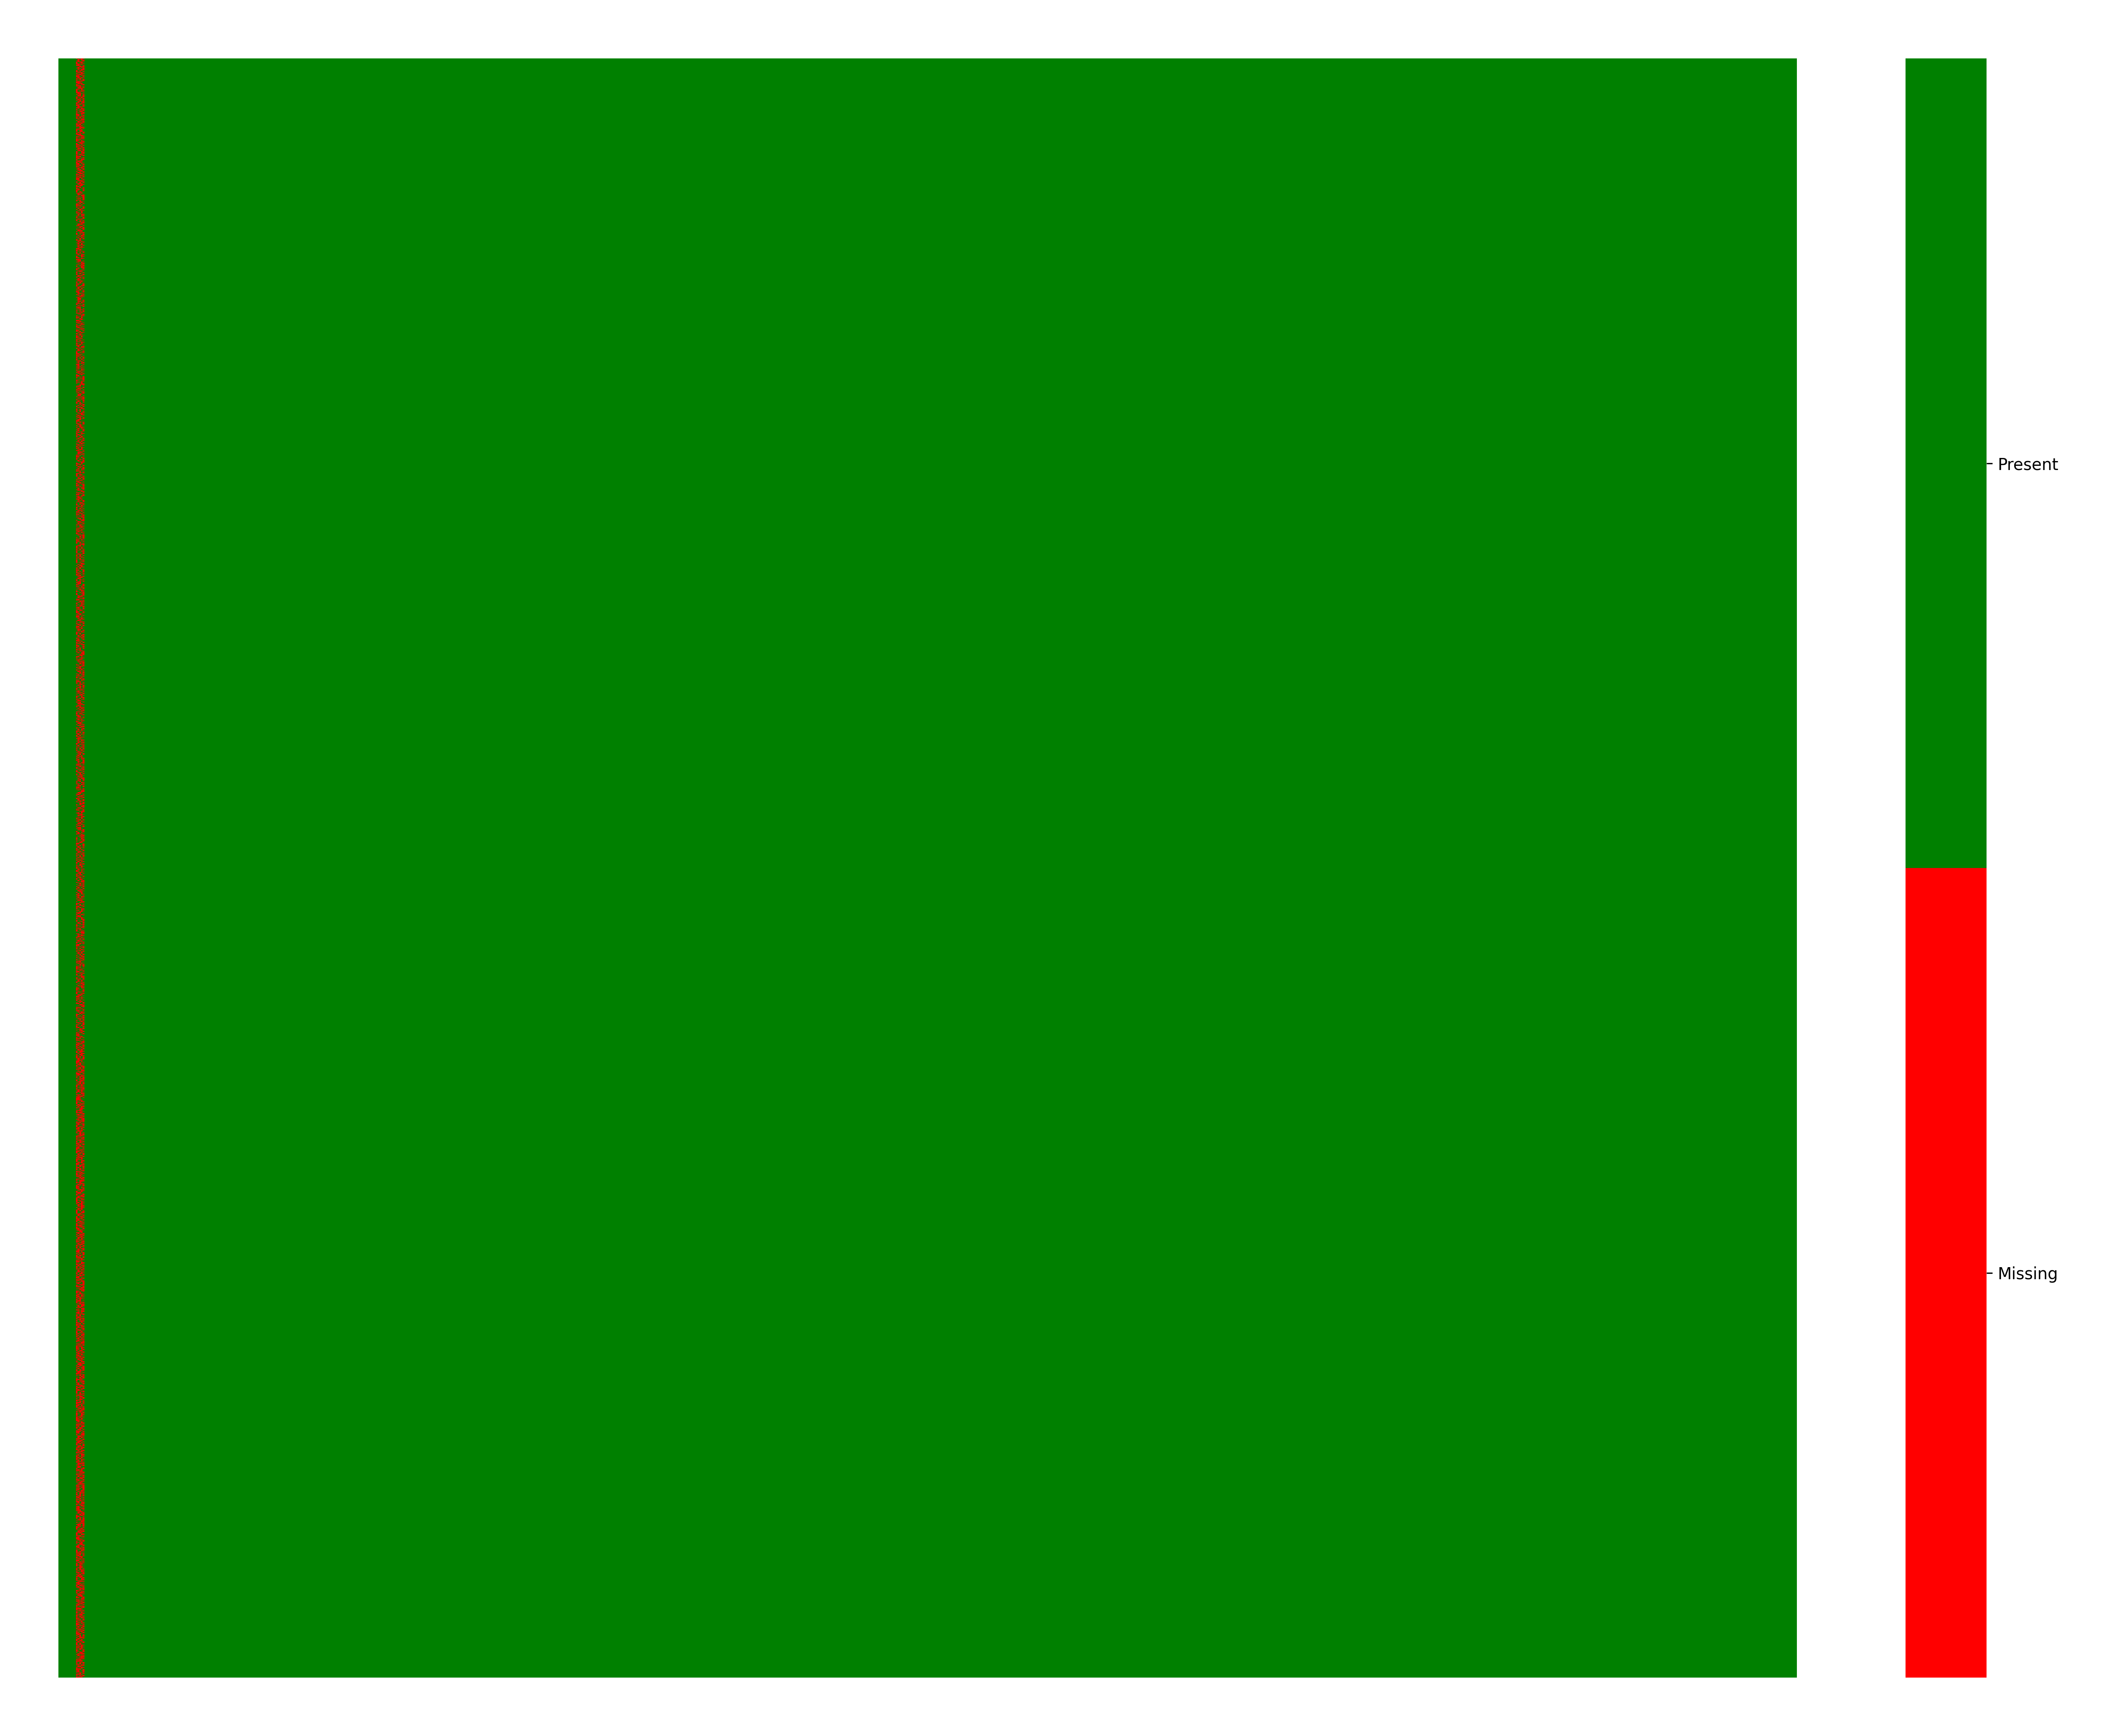
\includegraphics[width=\linewidth]{case4_v0.3_heatmap_cleaned.png}
        \caption{v0.3 (Worst)}
    \end{subfigure}
    \caption{Case 4 cleaned datasets comparison}
\end{figure}

\subsubsection{Case 5: MNAR – Moderate Dependency}

\textbf{Score Table:}

\begin{table}[H]
\centering
\caption{Scores by algorithm, Case 5}
\label{tab:score_algorithms_case5}
\begin{tabular}{|c|c|c|c|c|c|c|c|c|}
\hline
Algorithm & v0.0 & v0.1 & v0.2 & v0.3 & v0.4 & v0.5 & BnB & Average \\
\hline
Score & 67.1 & 60.0 & 64.5 & 55.0 & 60.0 & 60.0 & 60.0 & \textbf{60.94} \\
\hline
\end{tabular}
\end{table}

\textbf{Observations}\\
v0.0 is again the best algorithm with a score of 67.1, thanks to high Constraint Adherence (40/40) and Data Retention (20/20). v0.3 performs significantly worse (55.0), particularly in Missing Value Reduction (5.5/30) and Constraint Adherence (32.0/40). The gap is 12.1 points, again showing lower variance.  

\textbf{Heatmaps}\\
The input dataset displays a characteristic MNAR pattern with missing values concentrated in specific columns.

\begin{figure}[H]
    \centering
    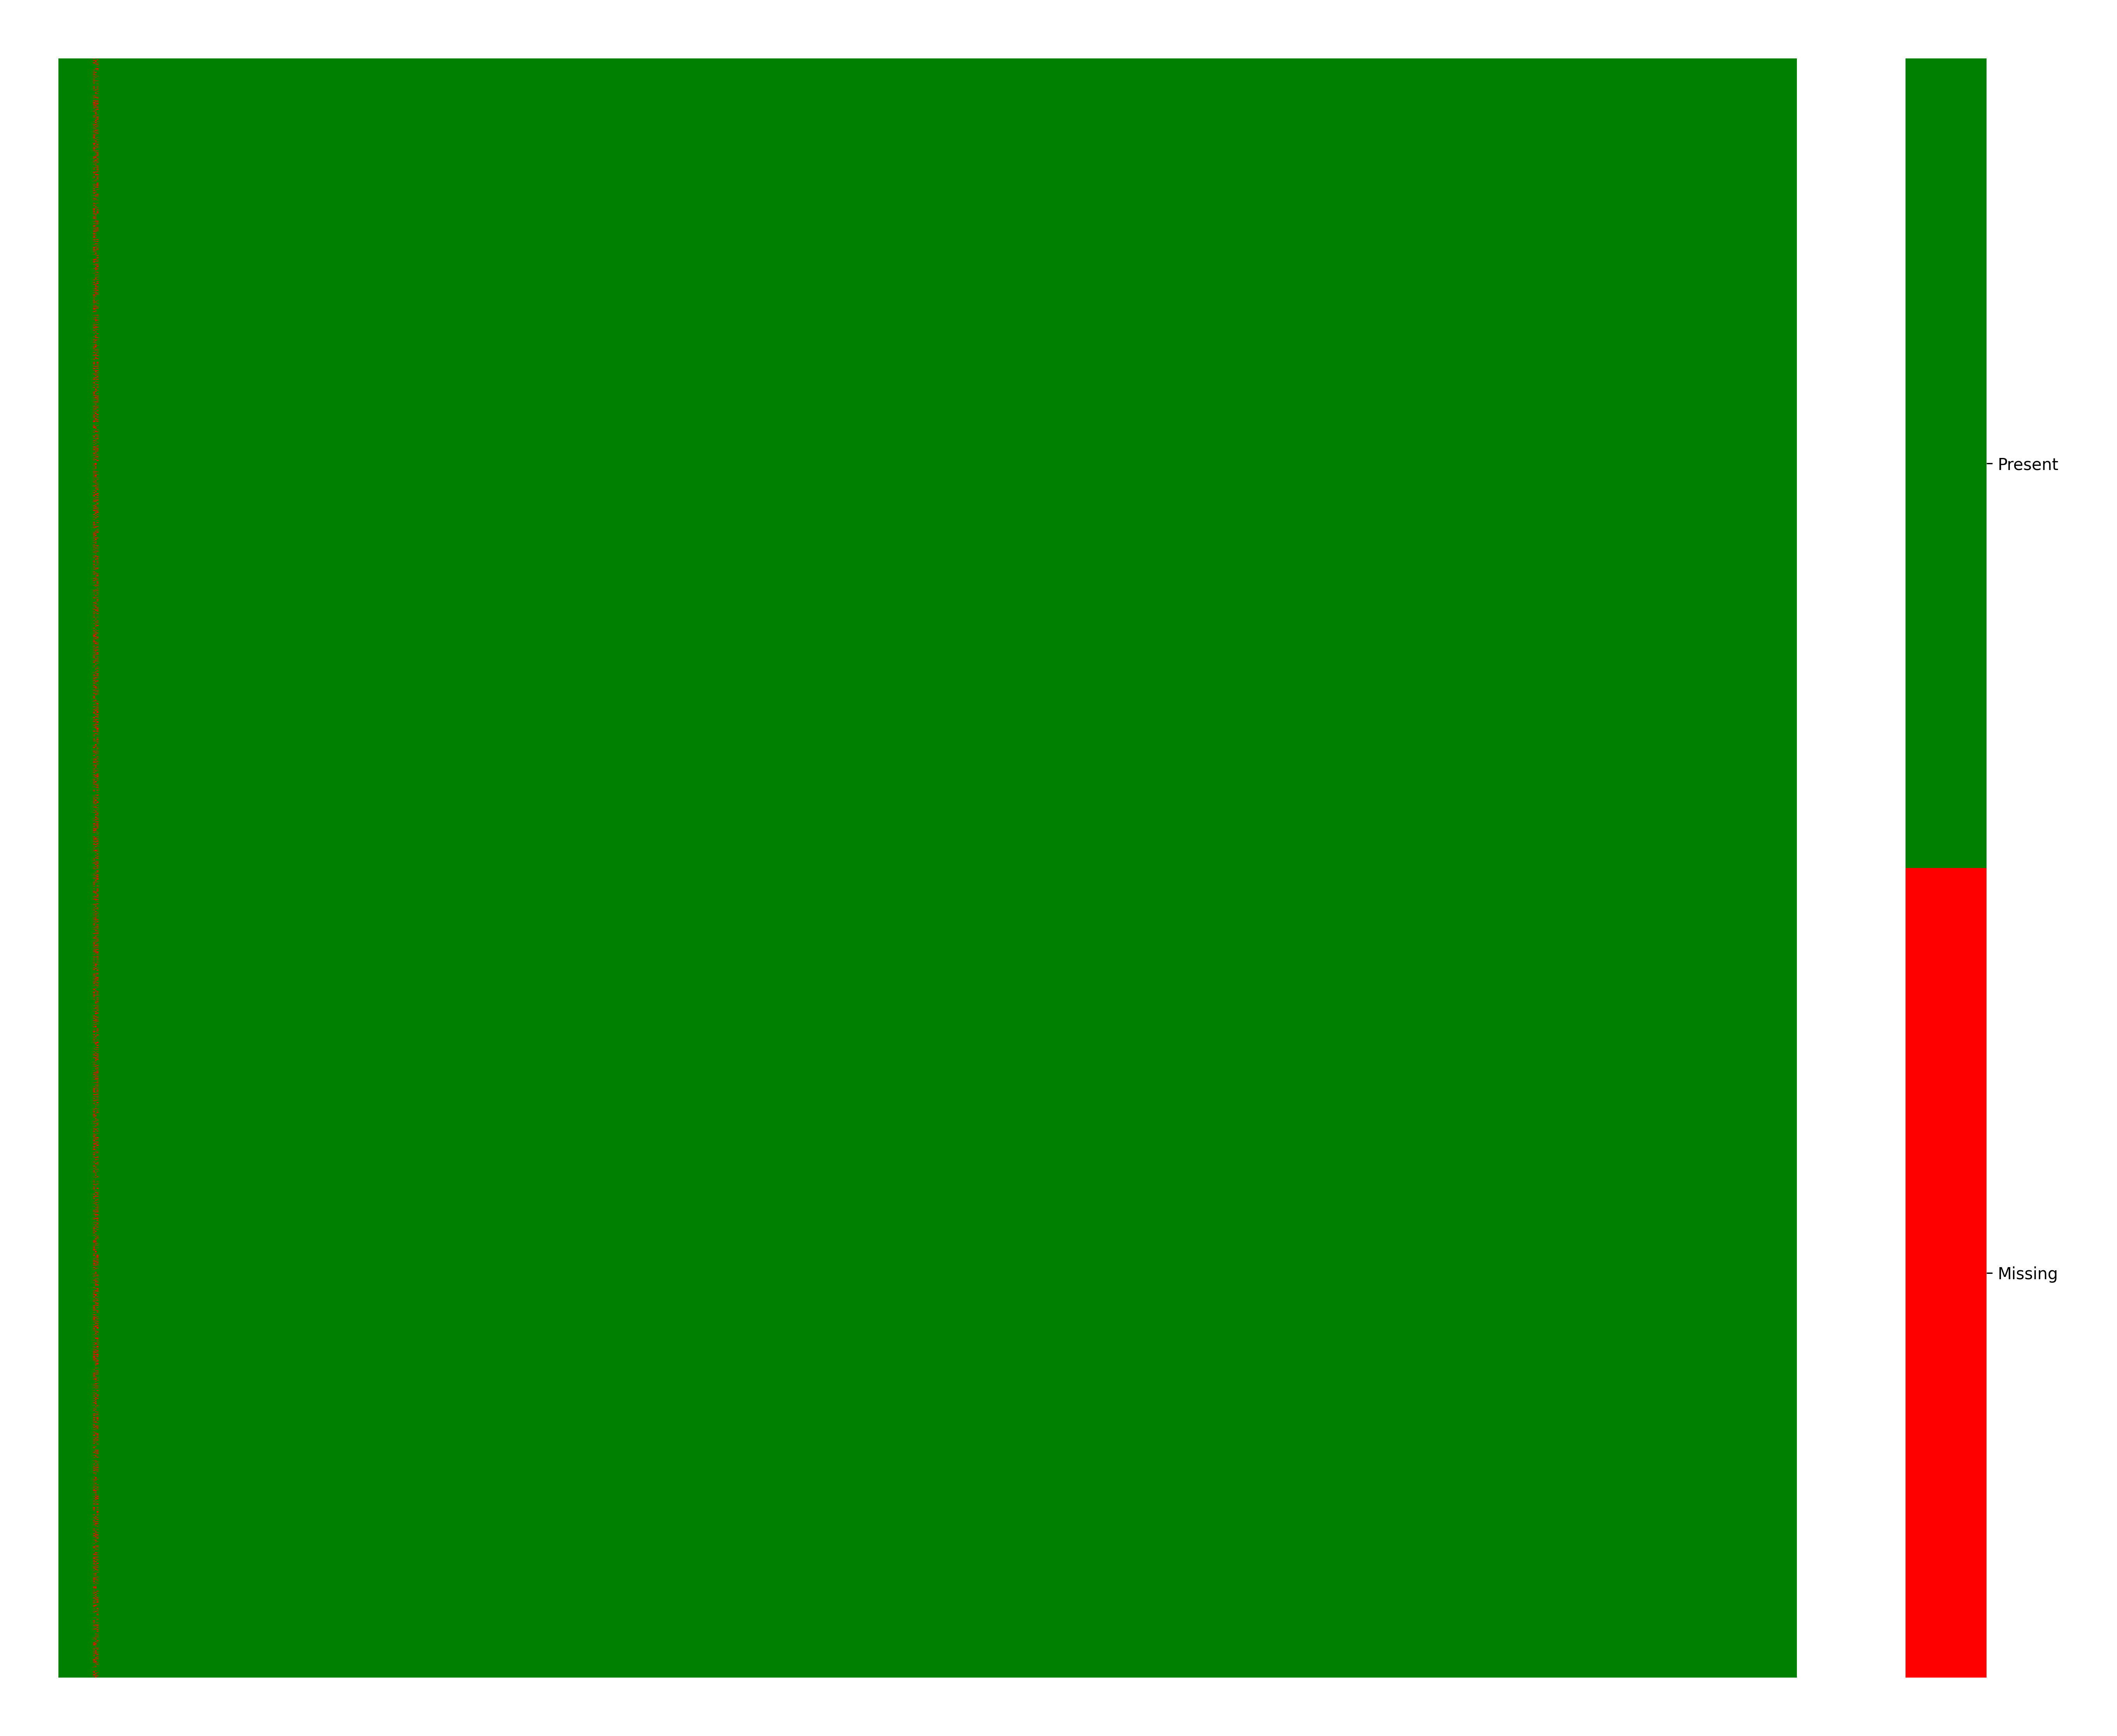
\includegraphics[width=0.5\linewidth]{case5_heatmap_erased.png}
    \caption{Case 5 Input Dataset}
\end{figure}

After applying v0.0, we see excellent preservation of missing regions with clear balance between erasing and preserving values. In contrast, v0.3 shows abrupt and inconsistent results.

\begin{figure}[H]
    \centering
    \begin{subfigure}{0.45\textwidth}
        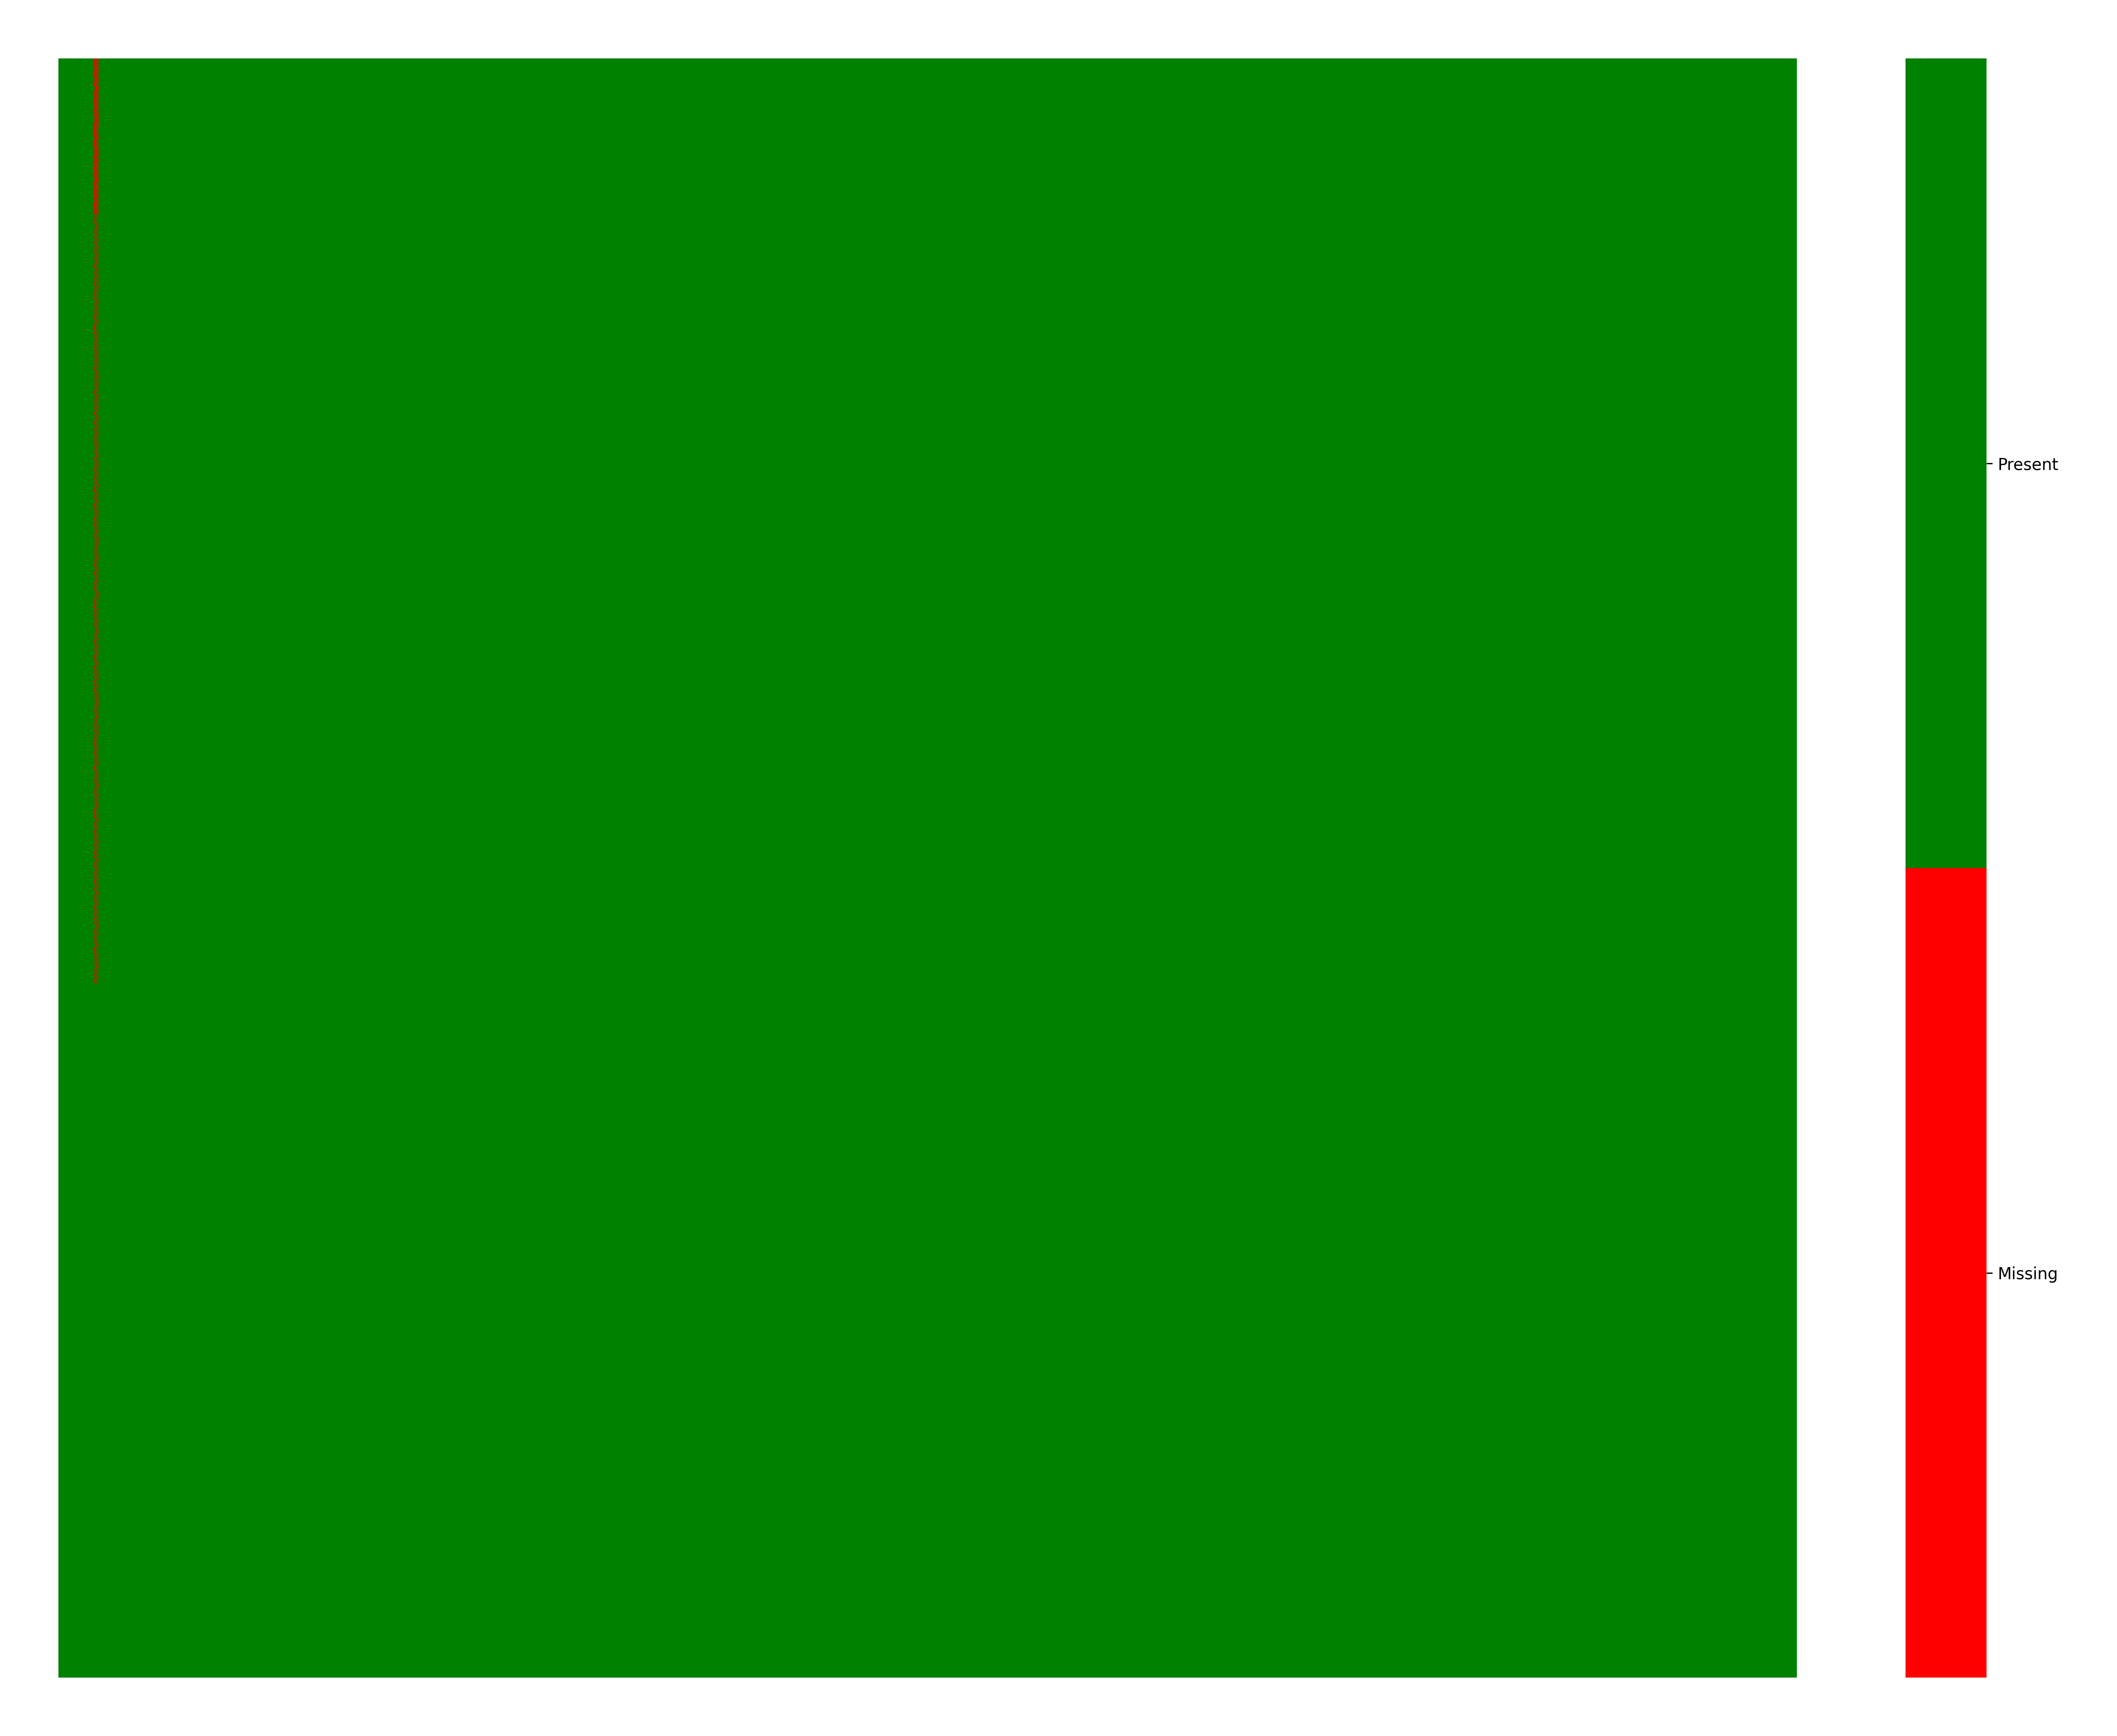
\includegraphics[width=\linewidth]{case5_v0.0_heatmap_cleaned.png}
        \caption{v0.0 (Best)}
    \end{subfigure}
    \hfill
    \begin{subfigure}{0.45\textwidth}
        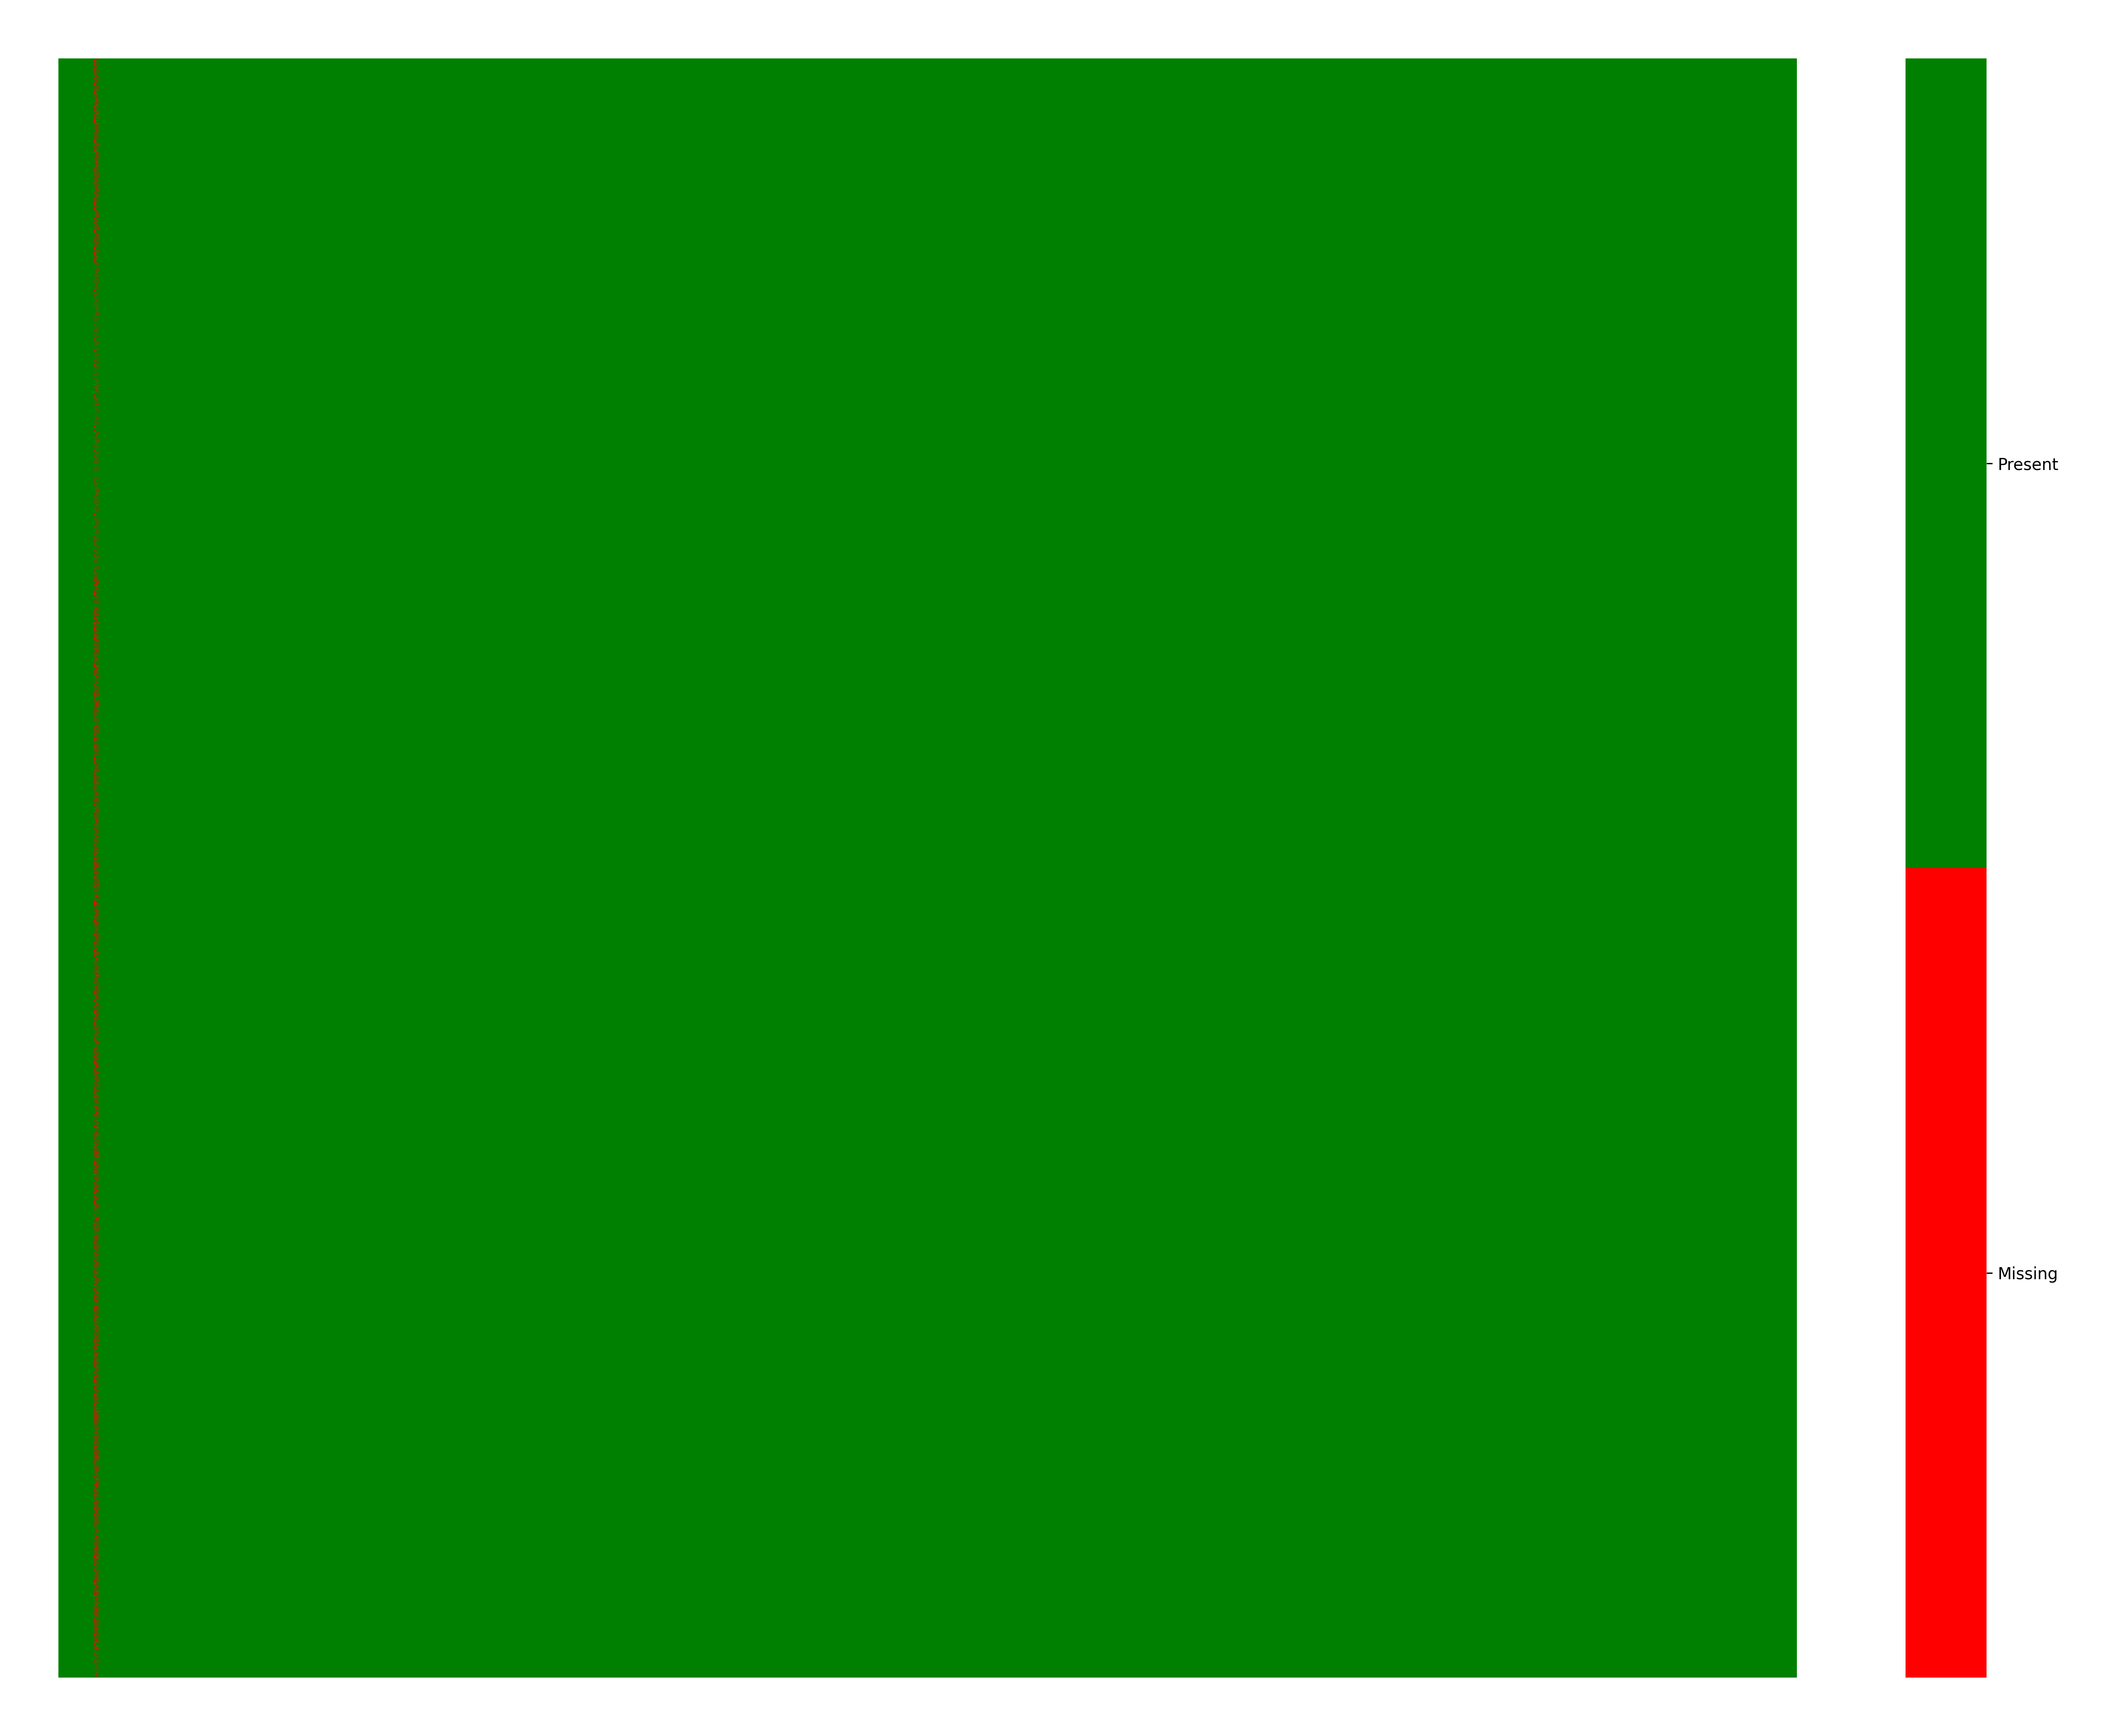
\includegraphics[width=\linewidth]{case5_v0.3_heatmap_cleaned.png}
        \caption{v0.3 (Worst)}
    \end{subfigure}
    \caption{Case 5 cleaned datasets comparison}
\end{figure}

\subsubsection{Case 6: MNAR – Strong Dependency}

\textbf{Score Table:}

\begin{table}[H]
\centering
\caption{Scores by algorithm, Case 6}
\label{tab:score_algorithms_case6}
\begin{tabular}{|c|c|c|c|c|c|c|c|c|}
\hline
Algorithm & v0.0 & v0.1 & v0.2 & v0.3 & v0.4 & v0.5 & BnB & Average \\
\hline
Score & 64.2 & 62.3 & 59.4 & 55.0 & 60.3 & 60.3 & 70.0 & \textbf{61.65} \\
\hline
\end{tabular}
\end{table}

\textbf{Observations}\\
BnB outperforms all other algorithms with a score of 70.0. It has perfect results in constraint adherence, retention, and bonus. The lowest score comes from v0.3 (55.0), with notably low adherence (24/40). The performance gap is 15 points. 

\textbf{Heatmaps}\\
The input dataset reflects a typical MNAR pattern with missing values concentrated across specific columns.

\begin{figure}[H]
    \centering
    
\includegraphics[width=0.5\linewidth]{case6_heatmap_erased.png}
    \caption{Case 6 Input Dataset}
\end{figure}

After applying BnB, there is significant reduction in missing values while maintaining the pattern. In contrast, v0.3 shows broken patterns and noise.

\begin{figure}[H]
    \centering
    \begin{subfigure}{0.45\textwidth}
        
\includegraphics[width=\linewidth]{case6_bnb_heatmap_cleaned.png}
        \caption{BnB (Best)}
    \end{subfigure}
    \hfill
    \begin{subfigure}{0.45\textwidth}
        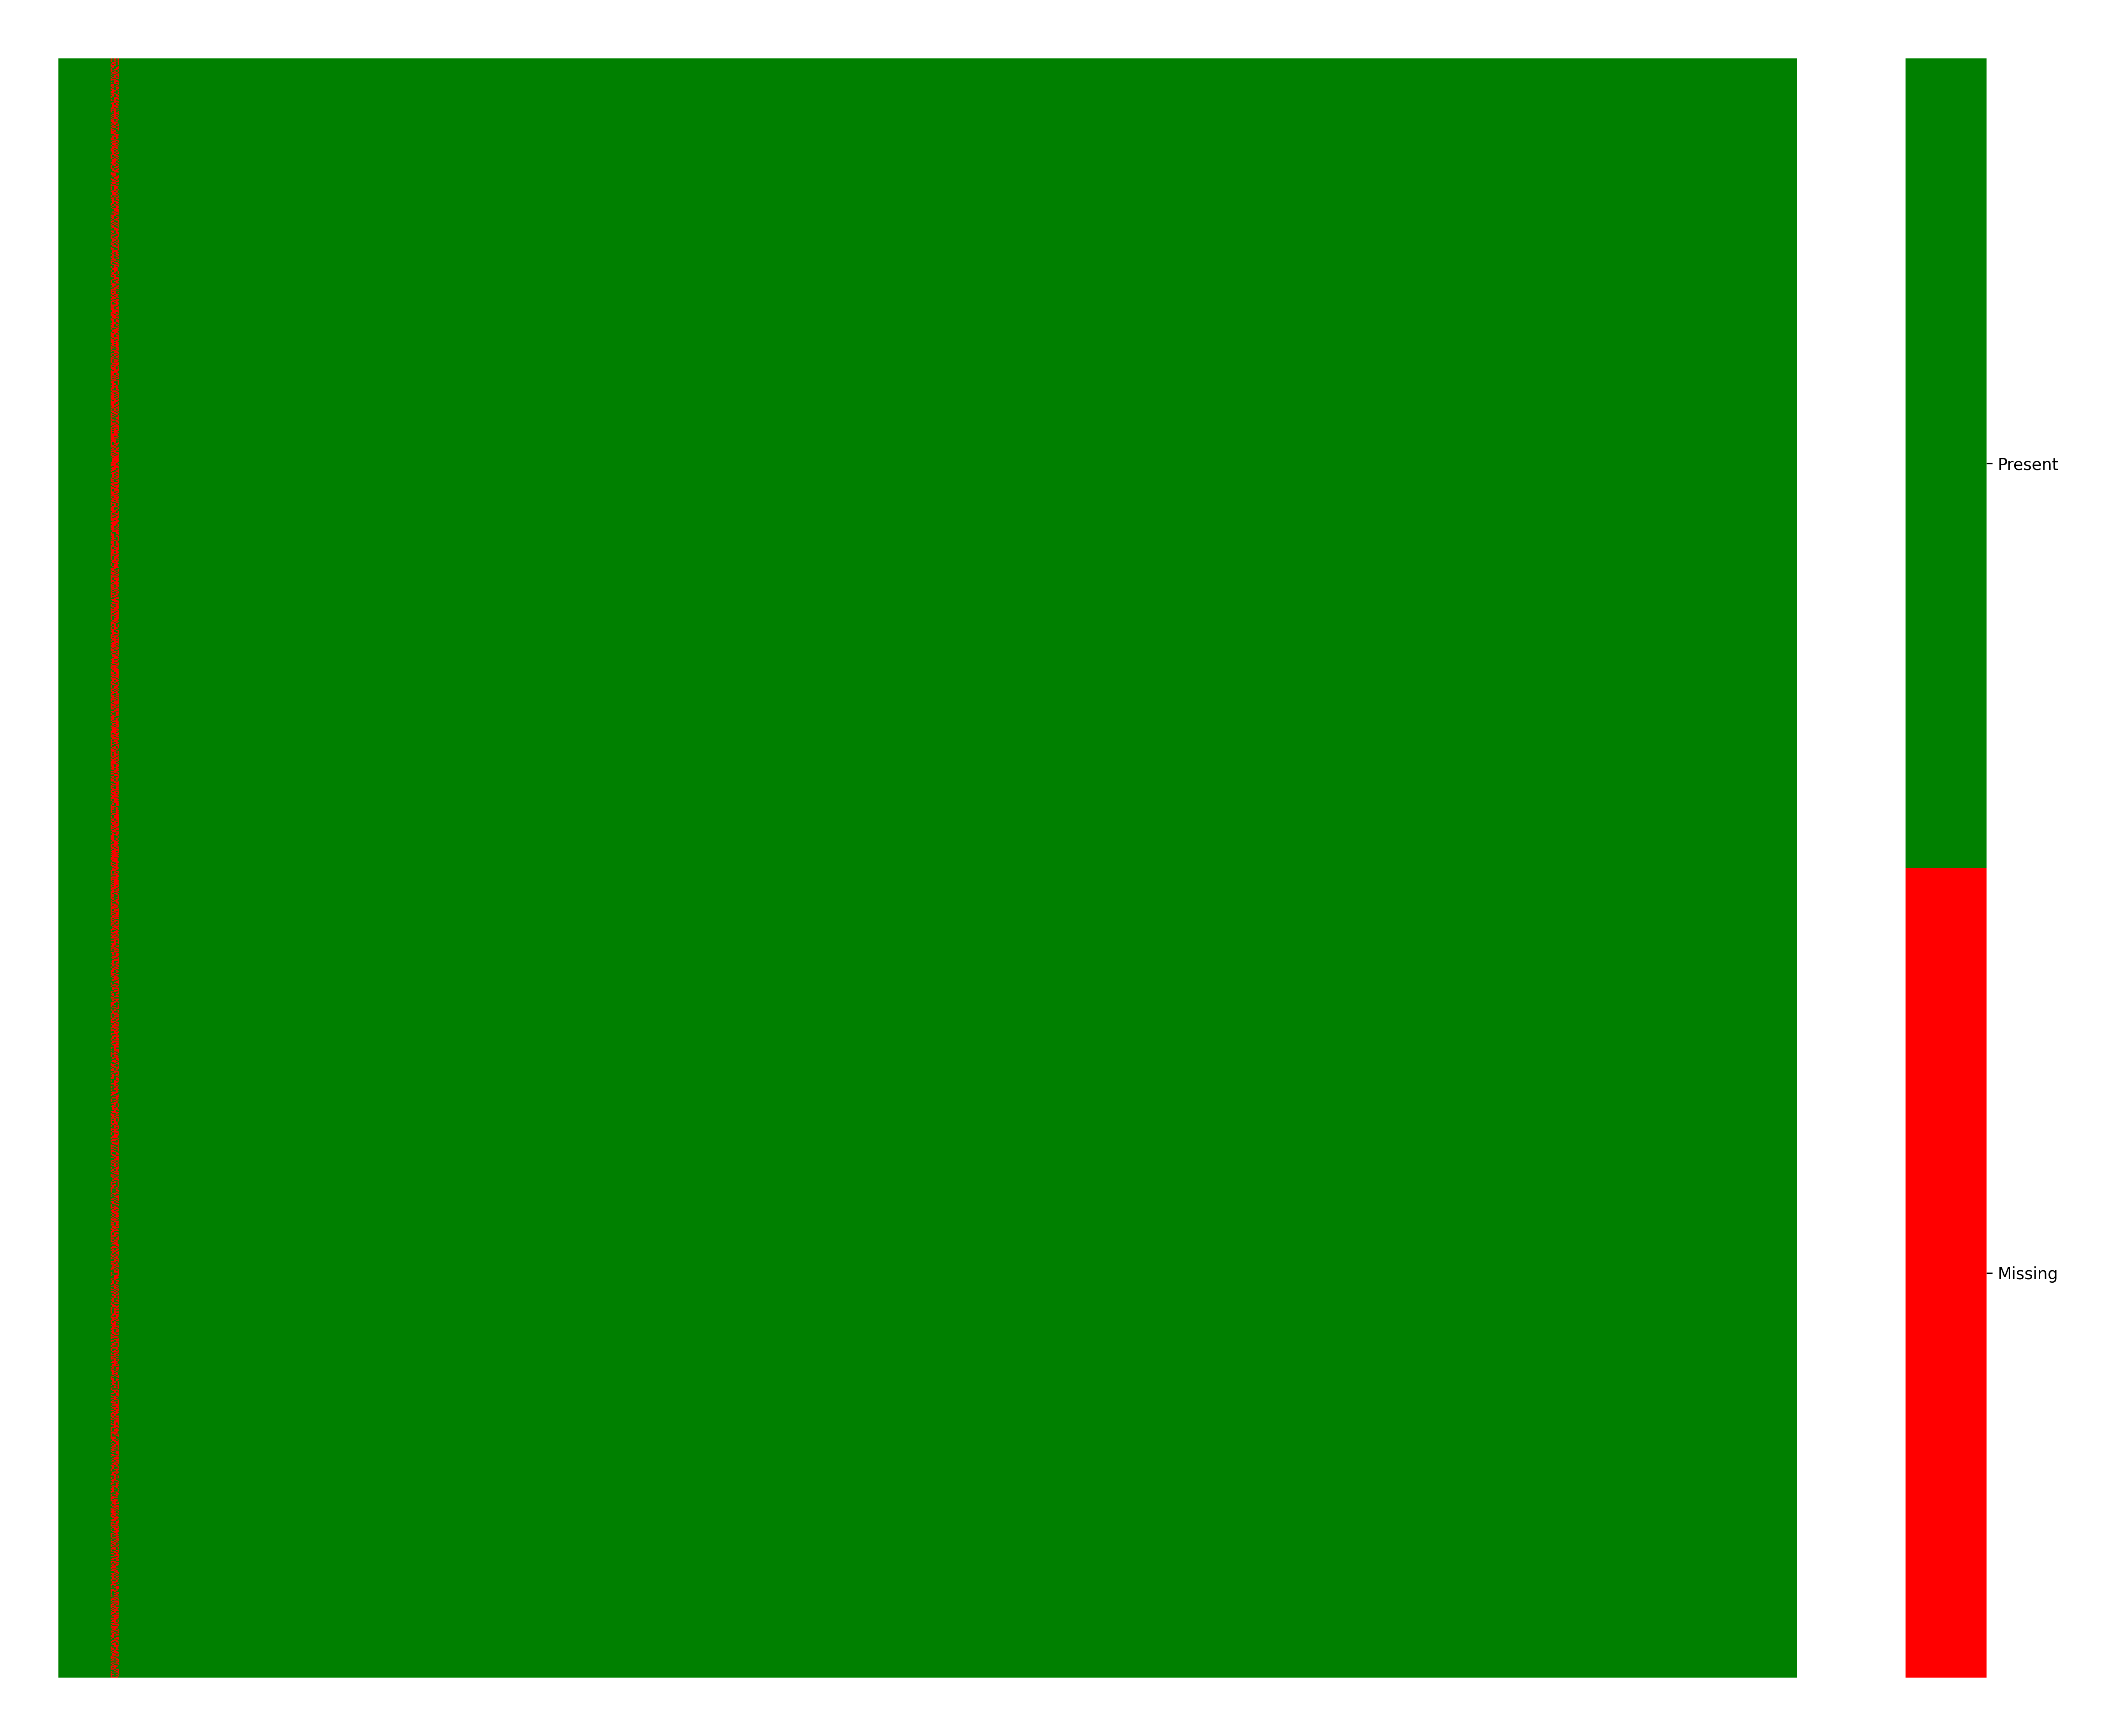
\includegraphics[width=\linewidth]{case6_v0.3_heatmap_cleaned.png}
        \caption{v0.3 (Worst)}
    \end{subfigure}
    \caption{Case 6 cleaned datasets comparison}
\end{figure}

\subsubsection{Case 7: MCAR – 15\% Missingness}

\textbf{Score Table:}

\begin{table}[H]
\centering
\caption{Scores by algorithm, Case 7}
\label{tab:score_algorithms_case7}
\begin{tabular}{|c|c|c|c|c|c|c|c|c|}
\hline
Algorithm & v0.0 & v0.1 & v0.2 & v0.3 & v0.4 & v0.5 & BnB & Average \\
\hline
Score & 55.5 & 53.9 & 50.2 & 62.0 & 84.8 & 84.8 & 52.0 & \textbf{63.33}  \\
\hline
\end{tabular}
\end{table}

\textbf{Observations}\\
The highest-performing algorithms are v0.4 and v0.5, each with a health score of 84.8. This is reflected in high Missing Value Reduction (27.3/30) and Constraint Adherence (40/40). The lowest score comes from v0.2 (50.2), due to very low Missing Value Reduction (8.1/30) and Constraint Adherence (24/40). The performance gap is 34.6 points, showing surprisingly high variance.

\textbf{Heatmaps}\\
We confirm the input dataset follows a uniform MCAR pattern.

\begin{figure}[H]
    \centering
    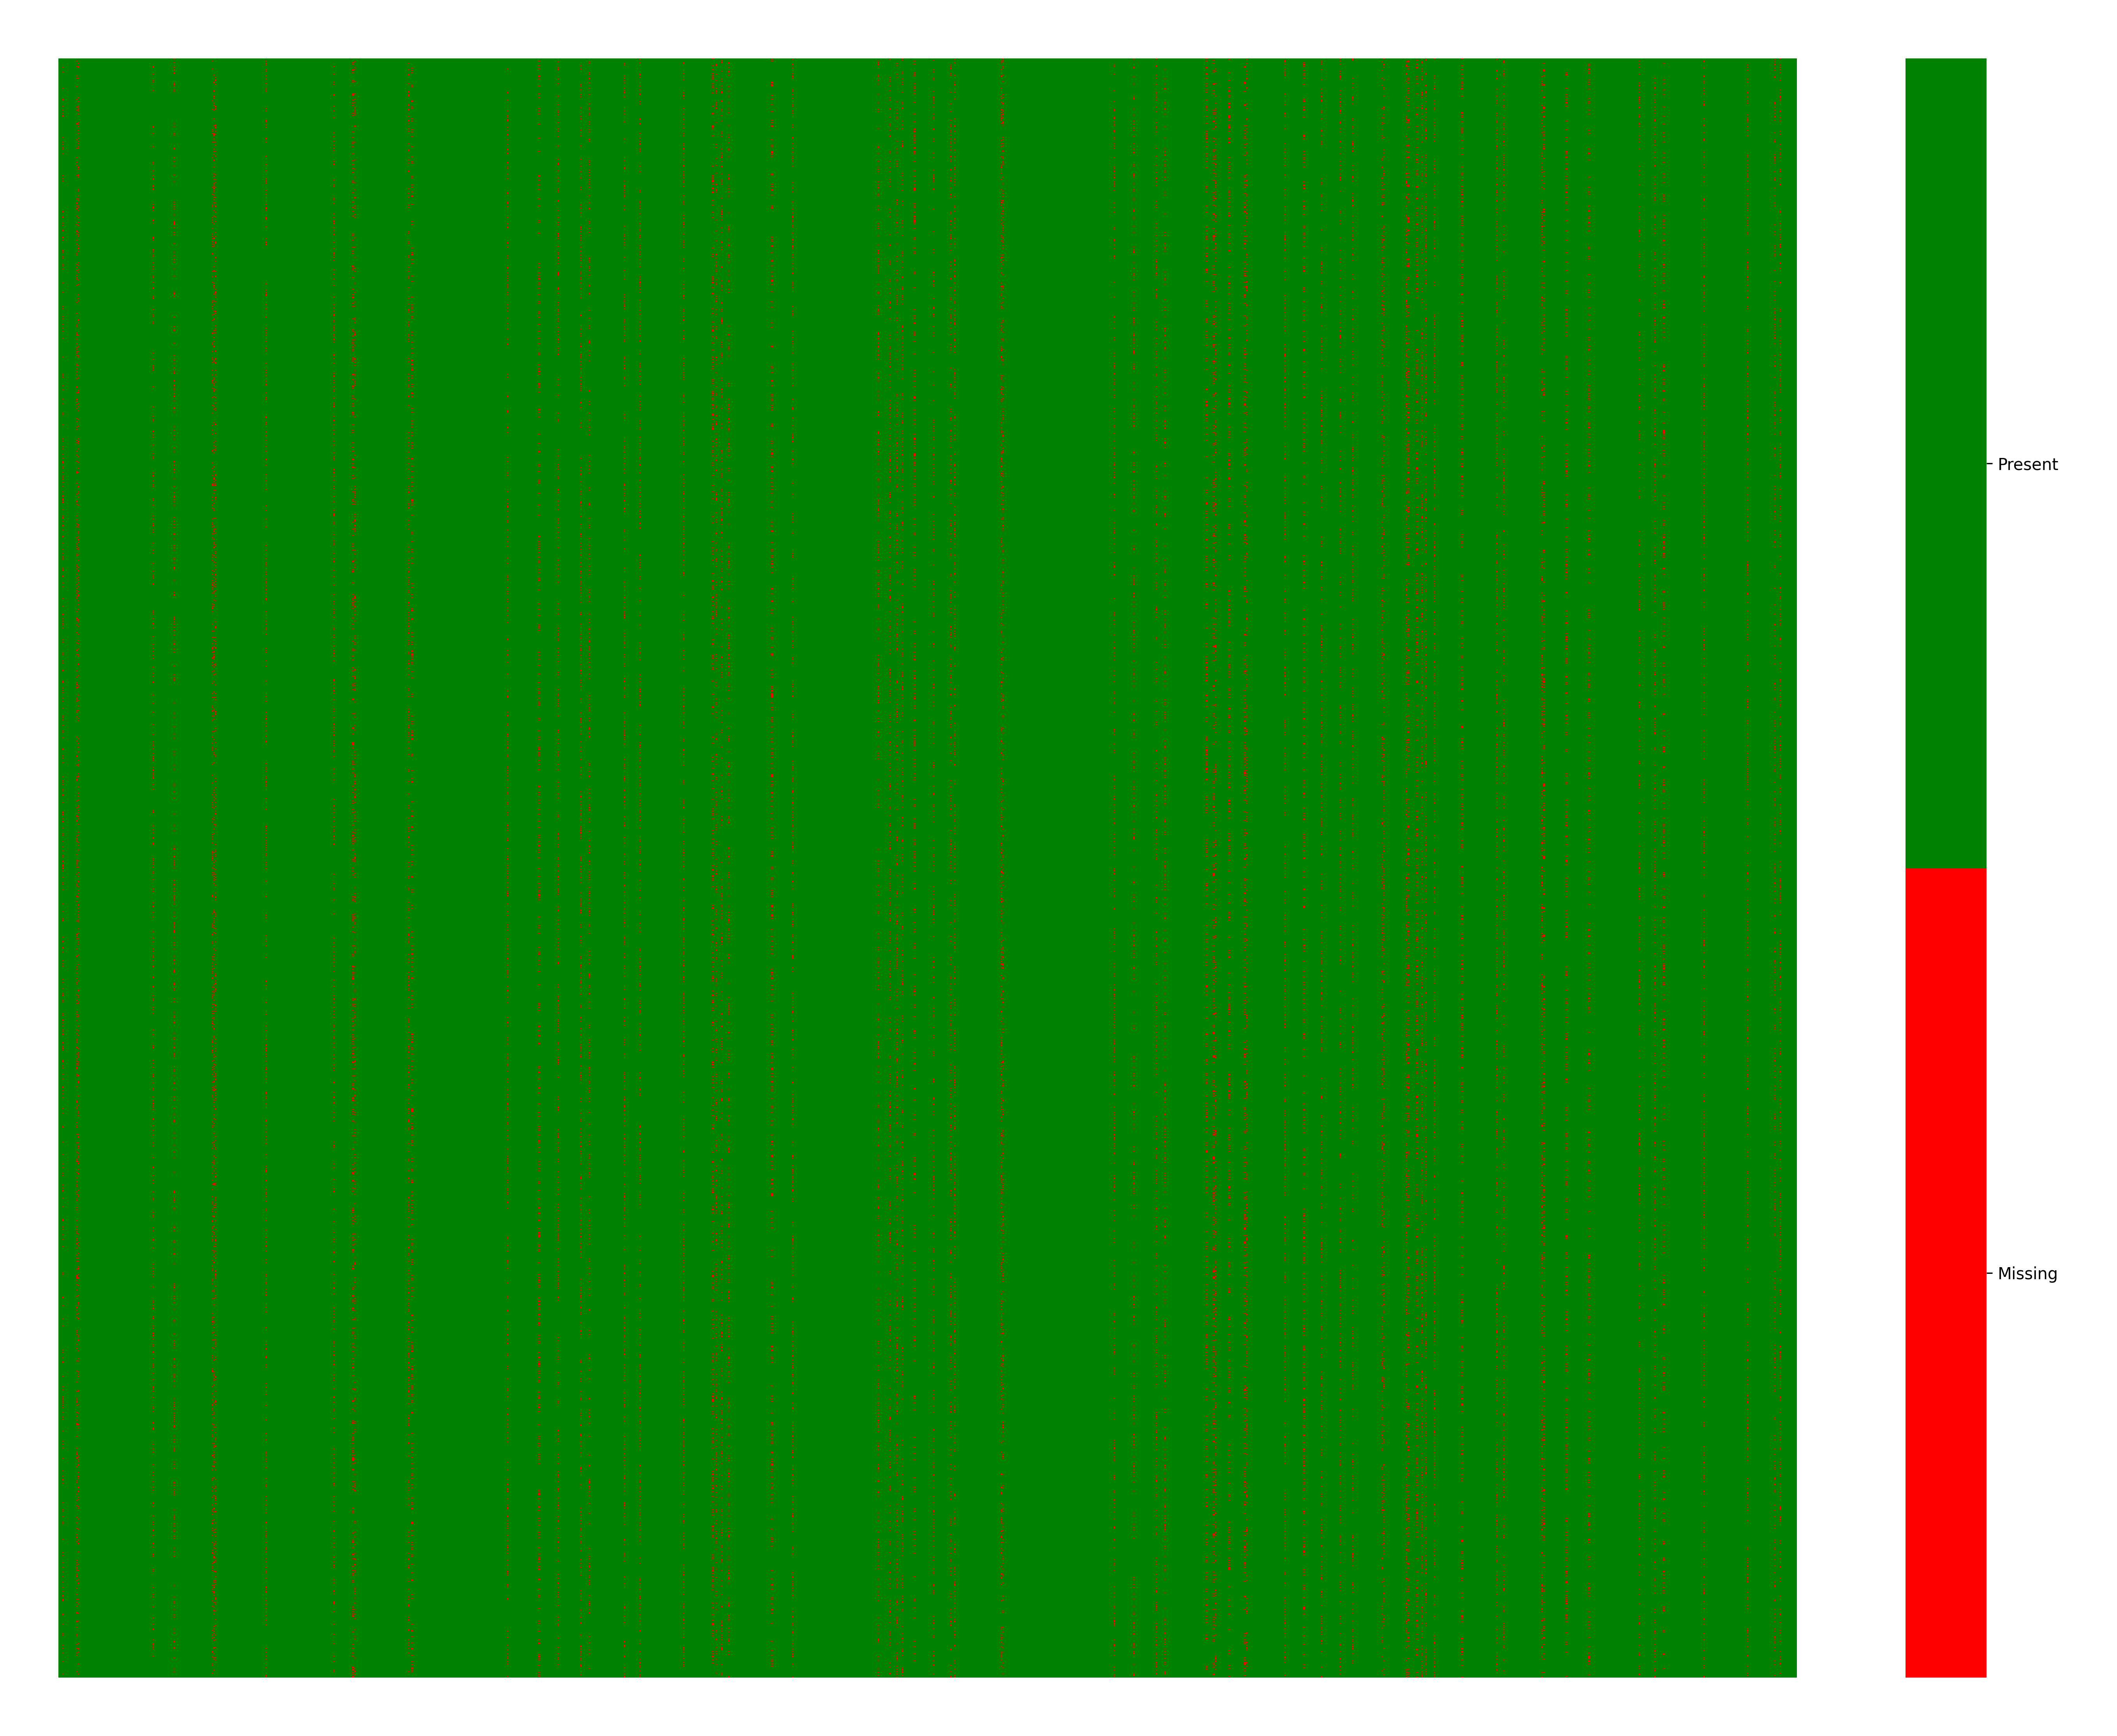
\includegraphics[width=0.5\linewidth]{case8_heatmap_erased.png}
    \caption{Case 7 Input Dataset}
\end{figure}

After applying v0.4 and v0.5, we see significant reduction in missing values, smoothing the MCAR distribution. In contrast, v0.2 shows erratic reconstructions and uneven density, highlighting its poor score.

\begin{figure}[H]
    \centering
    \begin{subfigure}{0.45\textwidth}
        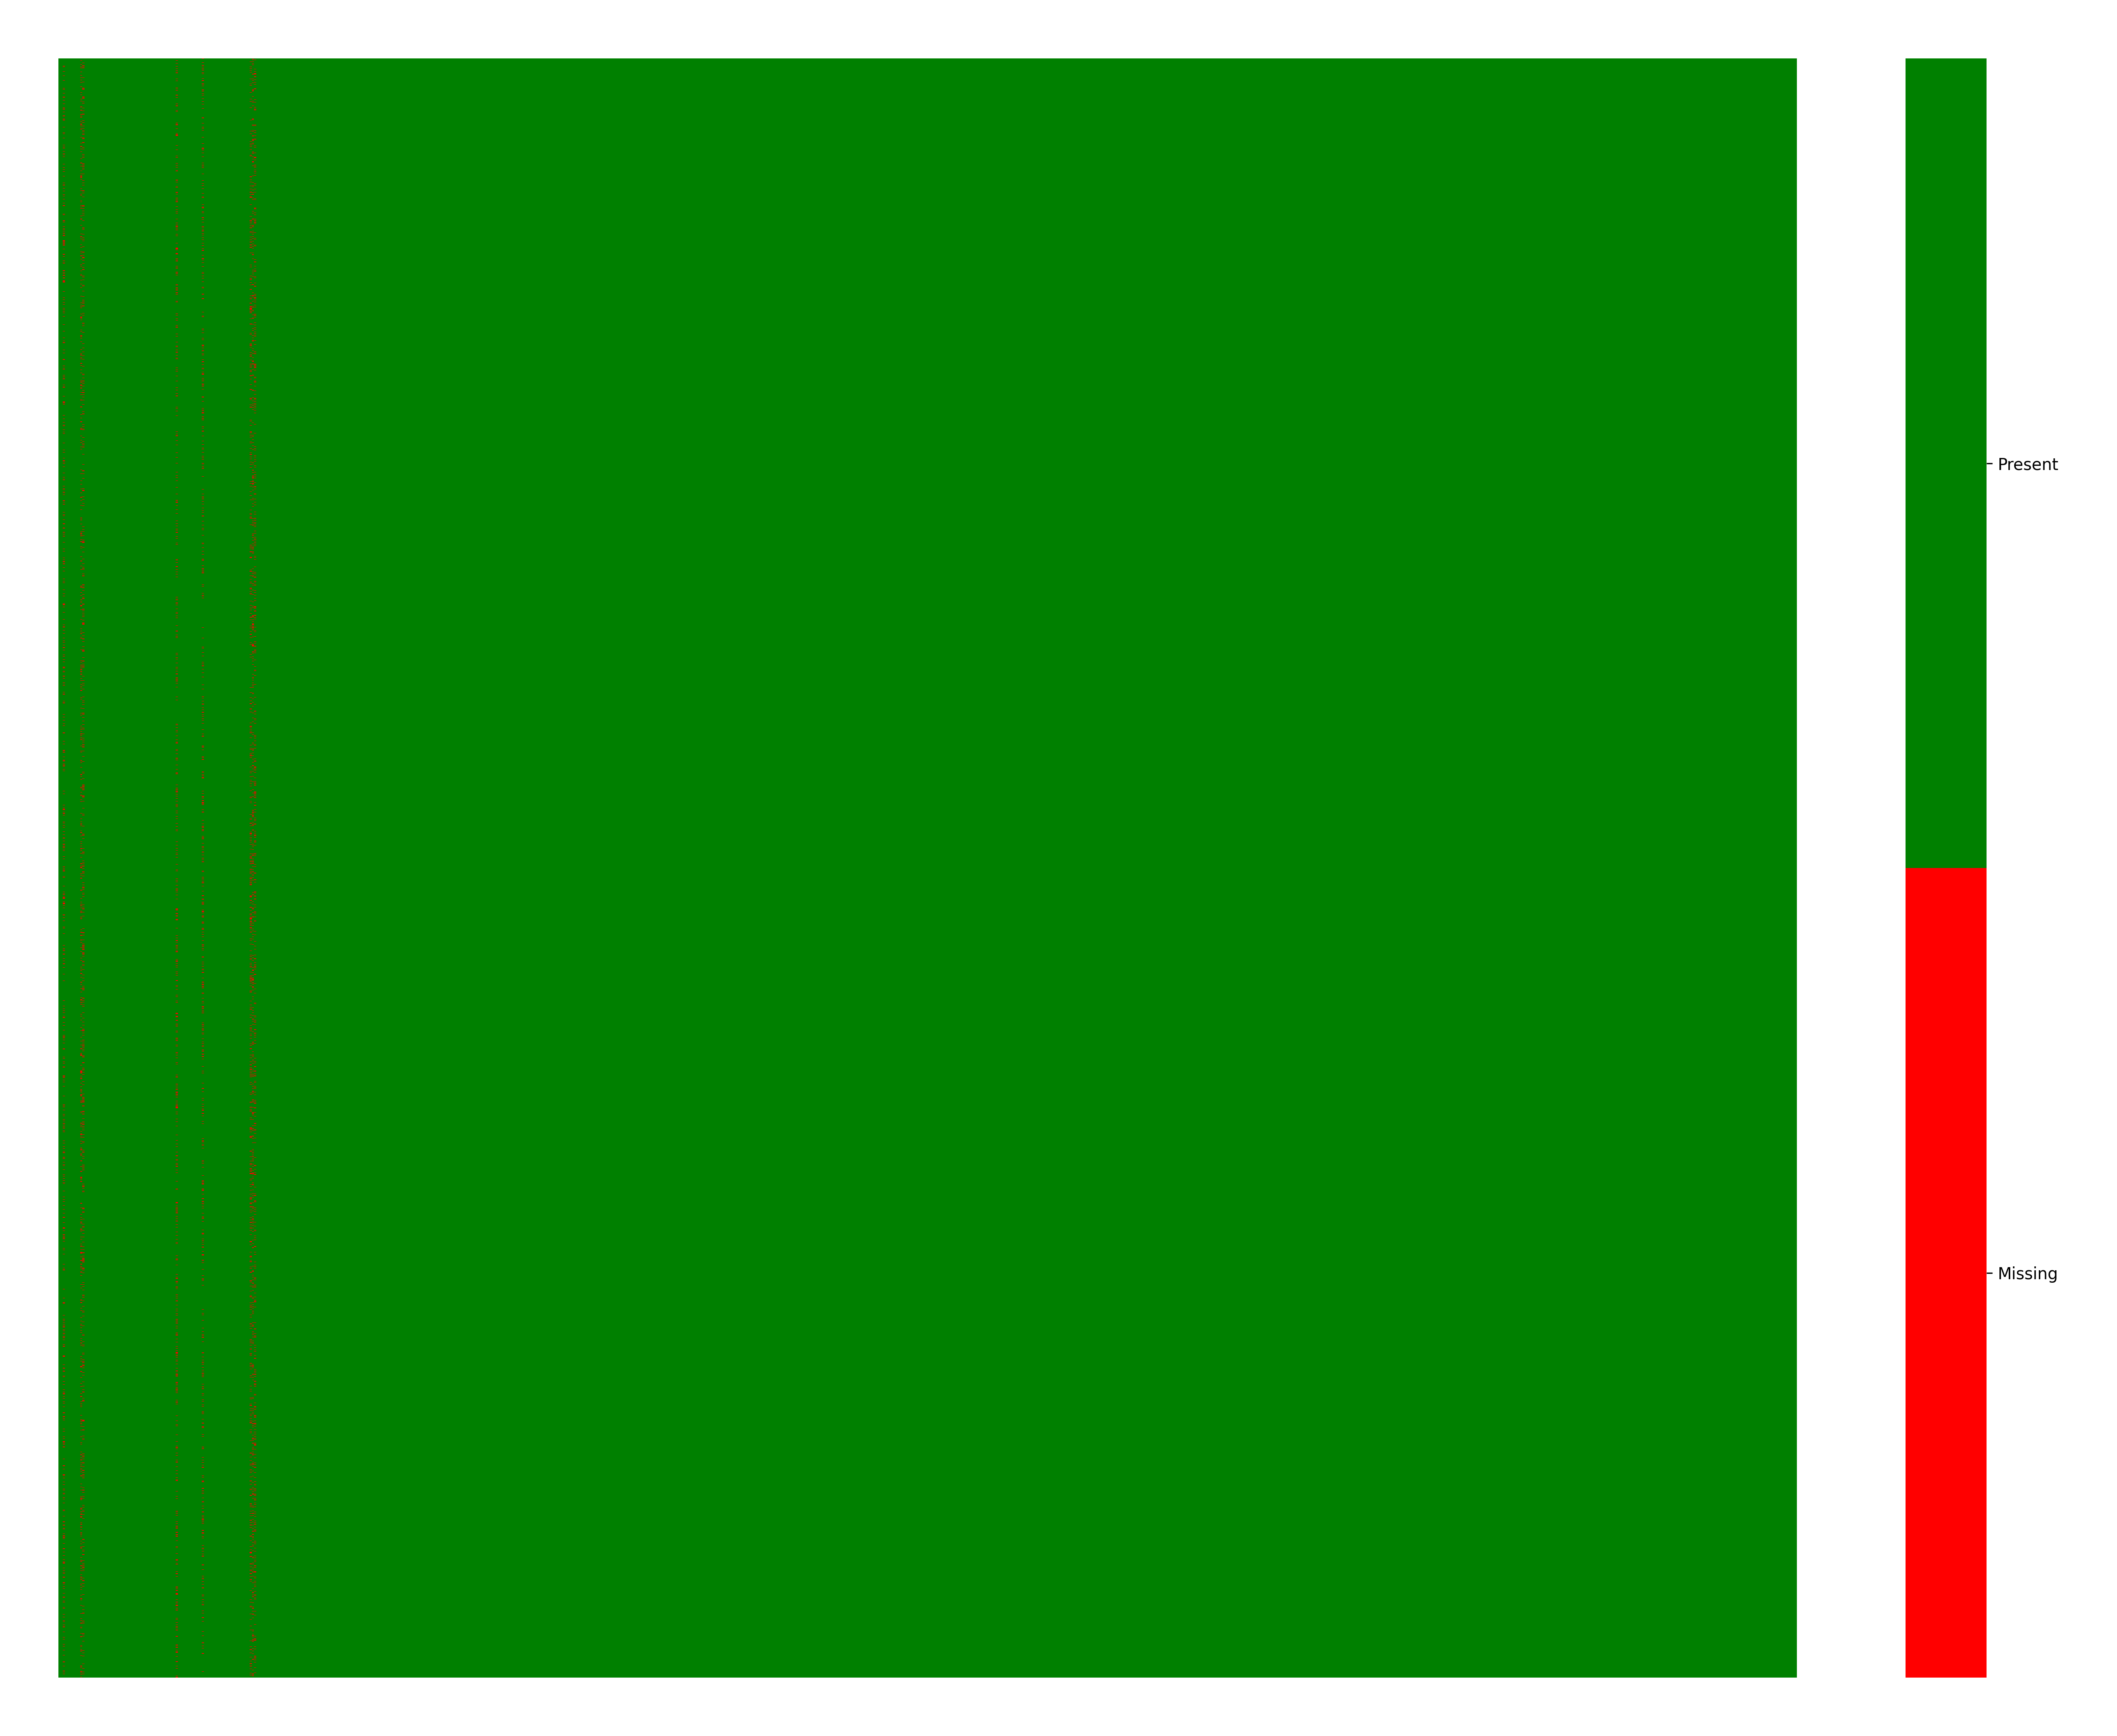
\includegraphics[width=\linewidth]{case8_v0.4_heatmap_cleaned.png}
        \caption{v0.4 (Best)}
    \end{subfigure}
    \hfill
    \begin{subfigure}{0.45\textwidth}
        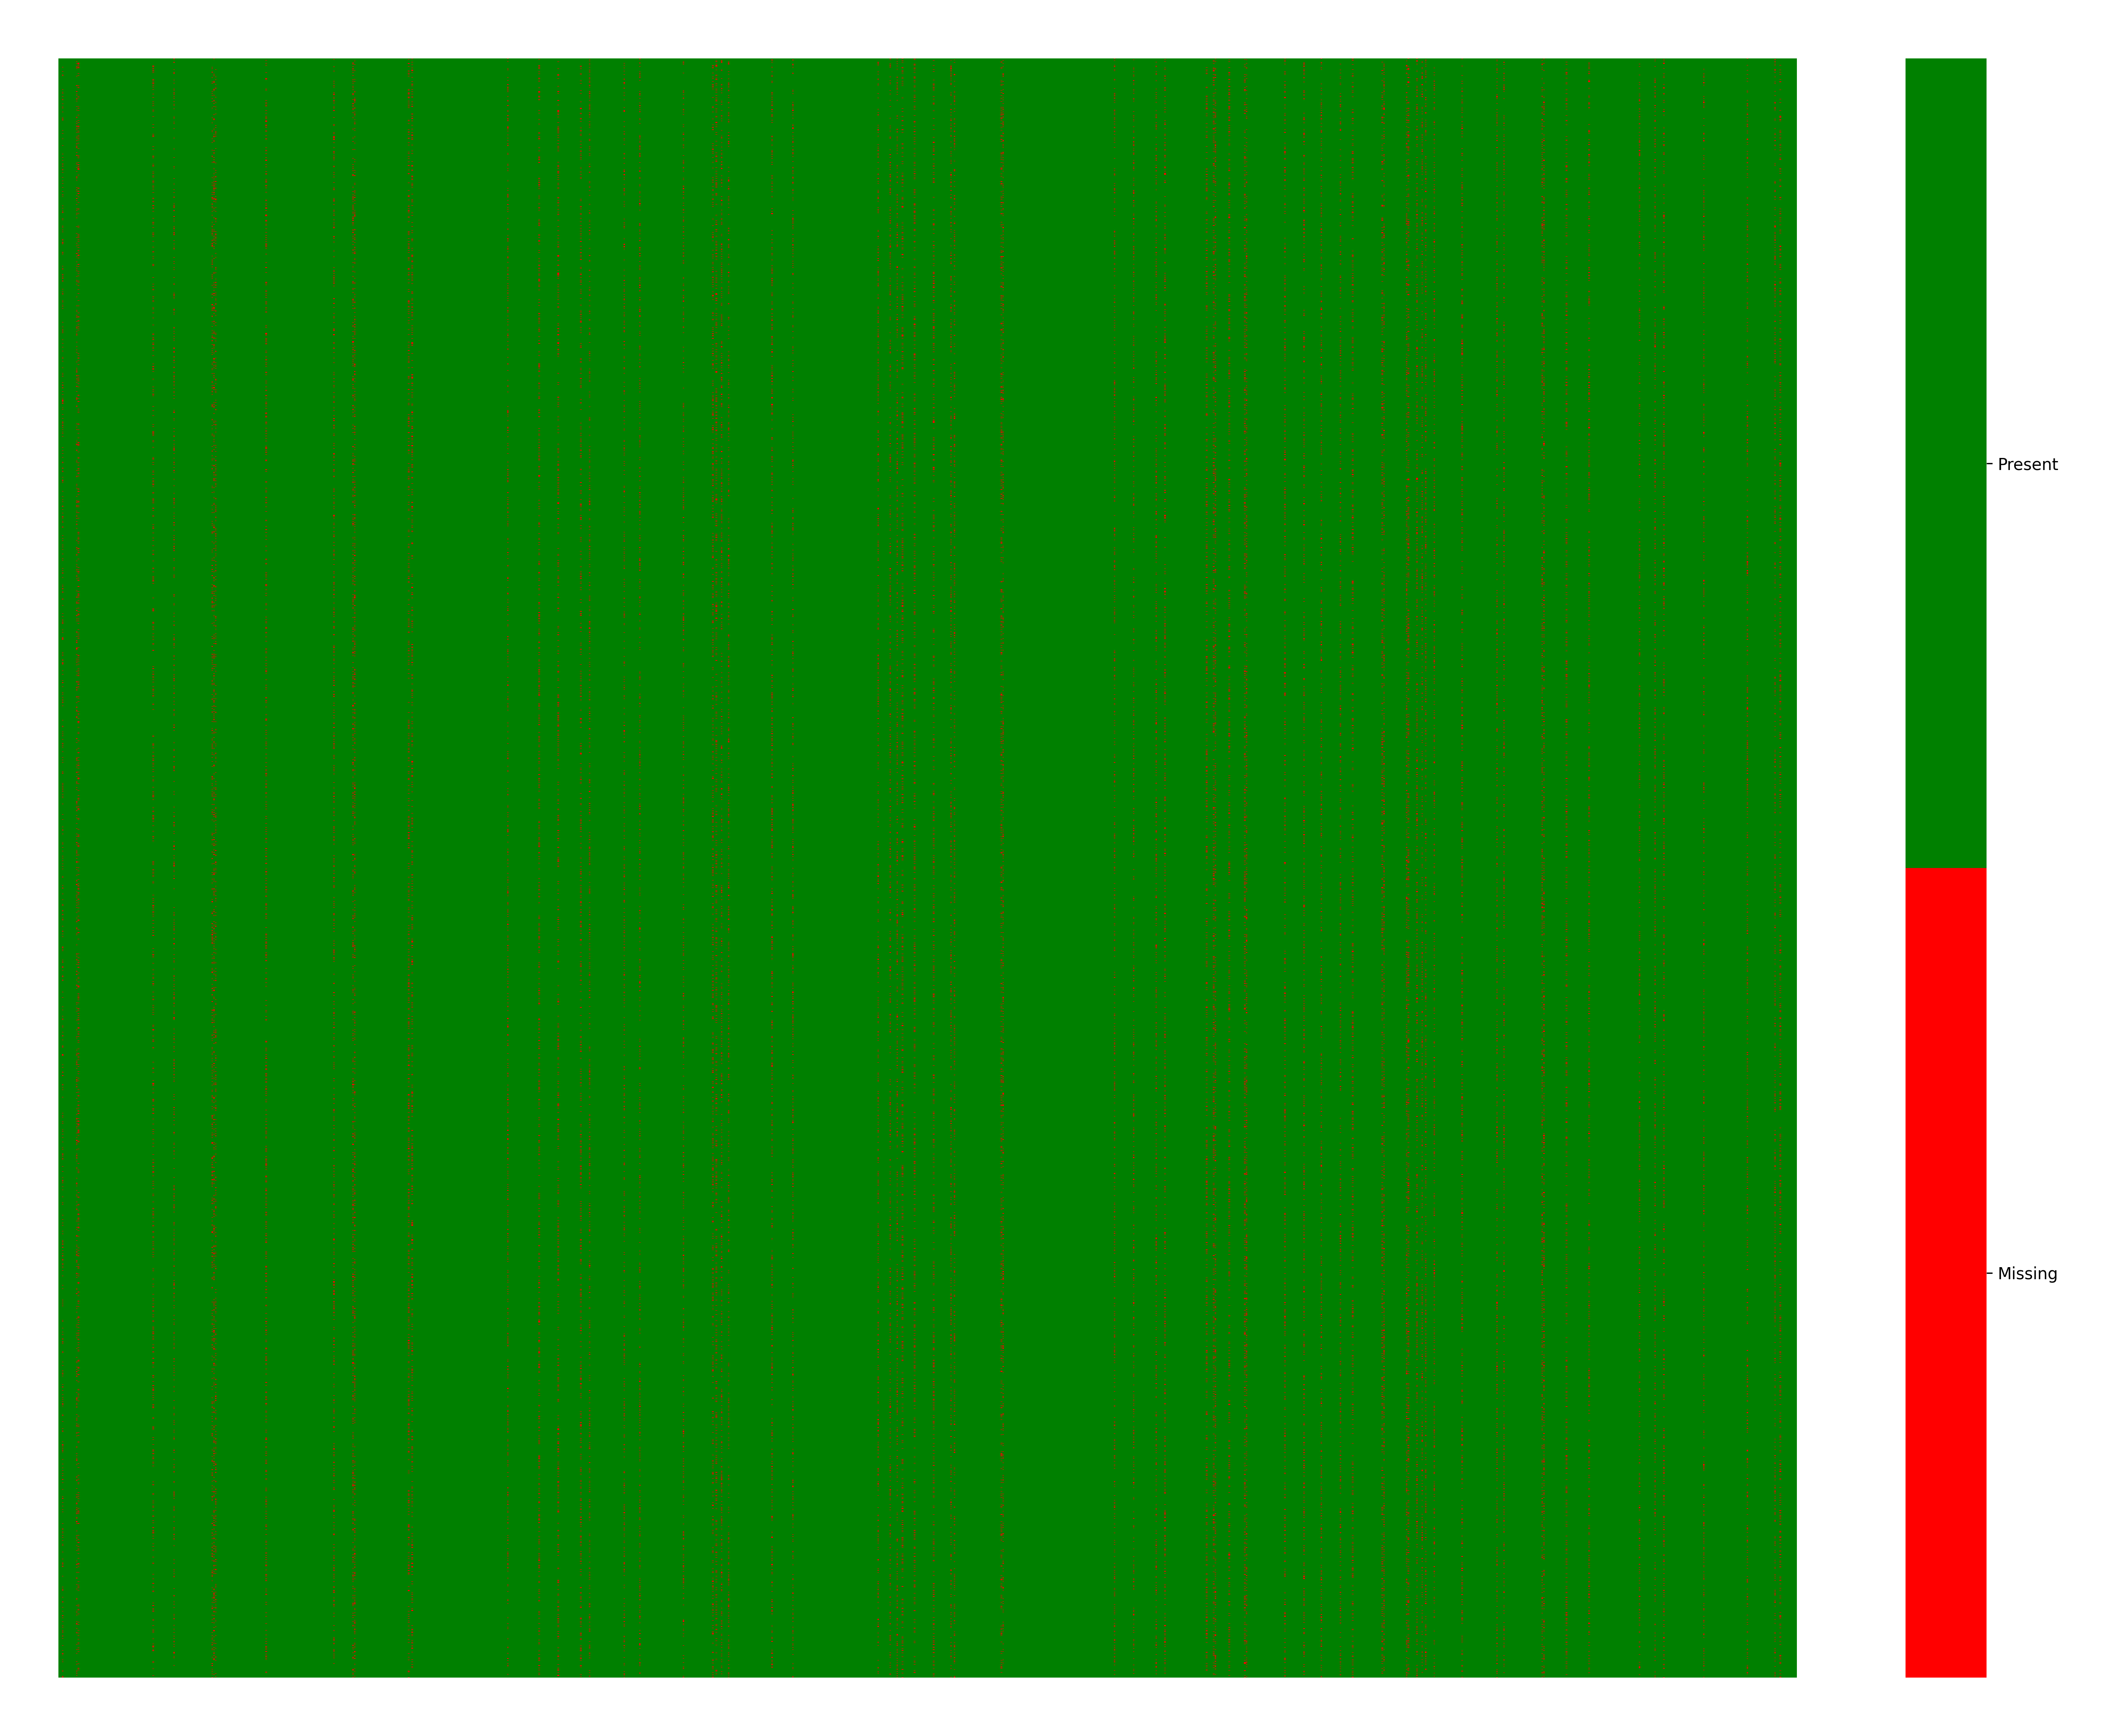
\includegraphics[width=\linewidth]{case8_v0.2_heatmap_cleaned.png}
        \caption{v0.2 (Worst)}
    \end{subfigure}
    \caption{Case 7 cleaned datasets comparison}
\end{figure}

\subsubsection{Case 8: MAR – Complex Dependency}

\textbf{Score Table:}

\begin{table}[H]
\centering
\caption{Scores by algorithm, Case 8}
\label{tab:score_algorithms_case8}
\begin{tabular}{|c|c|c|c|c|c|c|c|c|}
\hline
Algorithm & v0.0 & v0.1 & v0.2 & v0.3 & v0.4 & v0.5 & BnB & Average \\
\hline
Score & 65.4 & 62.9 & 60.0 & 57.5 & 60.9 & 60.9 & 70.0 & \textbf{62.51} \\
\hline
\end{tabular}
\end{table}

\textbf{Observations}\\
BnB outperforms all other algorithms with a score of 70.0. It has perfect results in constraint adherence, retention, and bonus. The lowest score comes from v0.3 (57.5), with notably low adherence (32/40) and Data Retention (15.7/20). The performance gap is 12.5 points, again showing lower variance. 

\textbf{Heatmaps}\\
The input dataset reflects a typical MAR pattern with missing values concentrated across specific columns.

\begin{figure}[H]
    \centering
    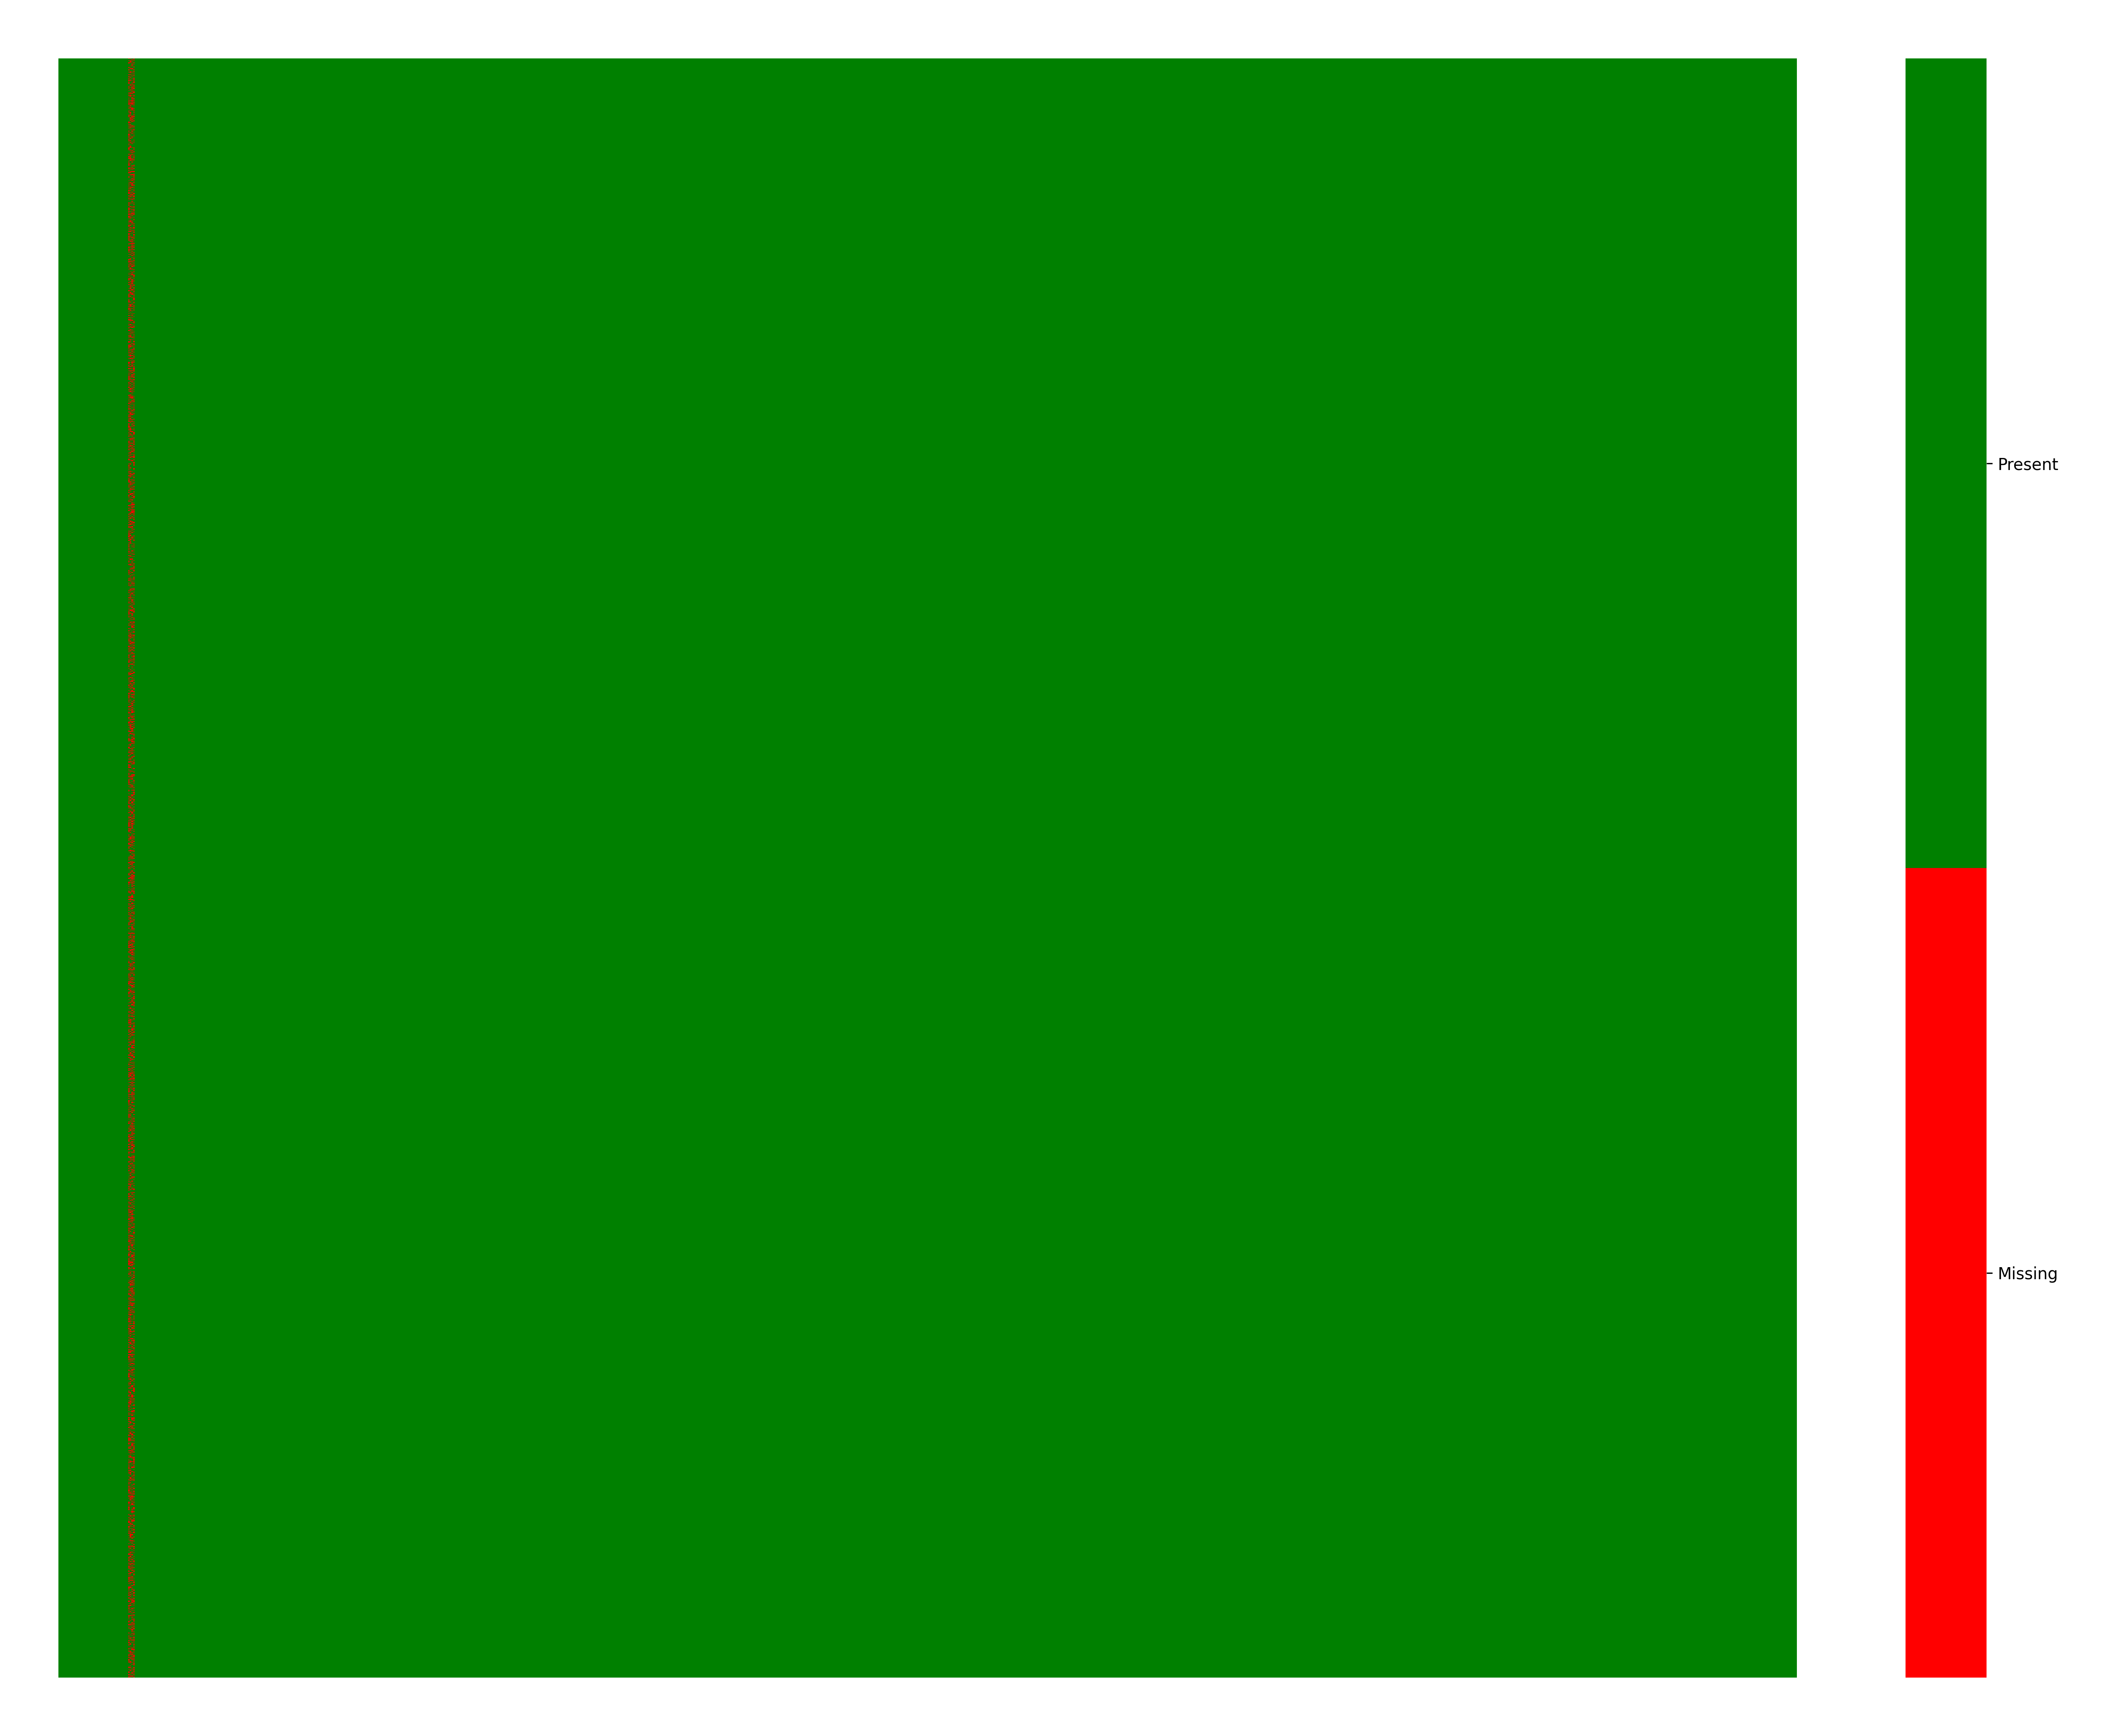
\includegraphics[width=0.5\linewidth]{case9_heatmap_erased.png}
    \caption{Case 8 Input Dataset}
\end{figure}

After applying BnB, missing values are reduced while column logic is maintained. In contrast, v0.3 shows problems from violated dependencies.

\begin{figure}[H]
    \centering
    \begin{subfigure}{0.45\textwidth}
        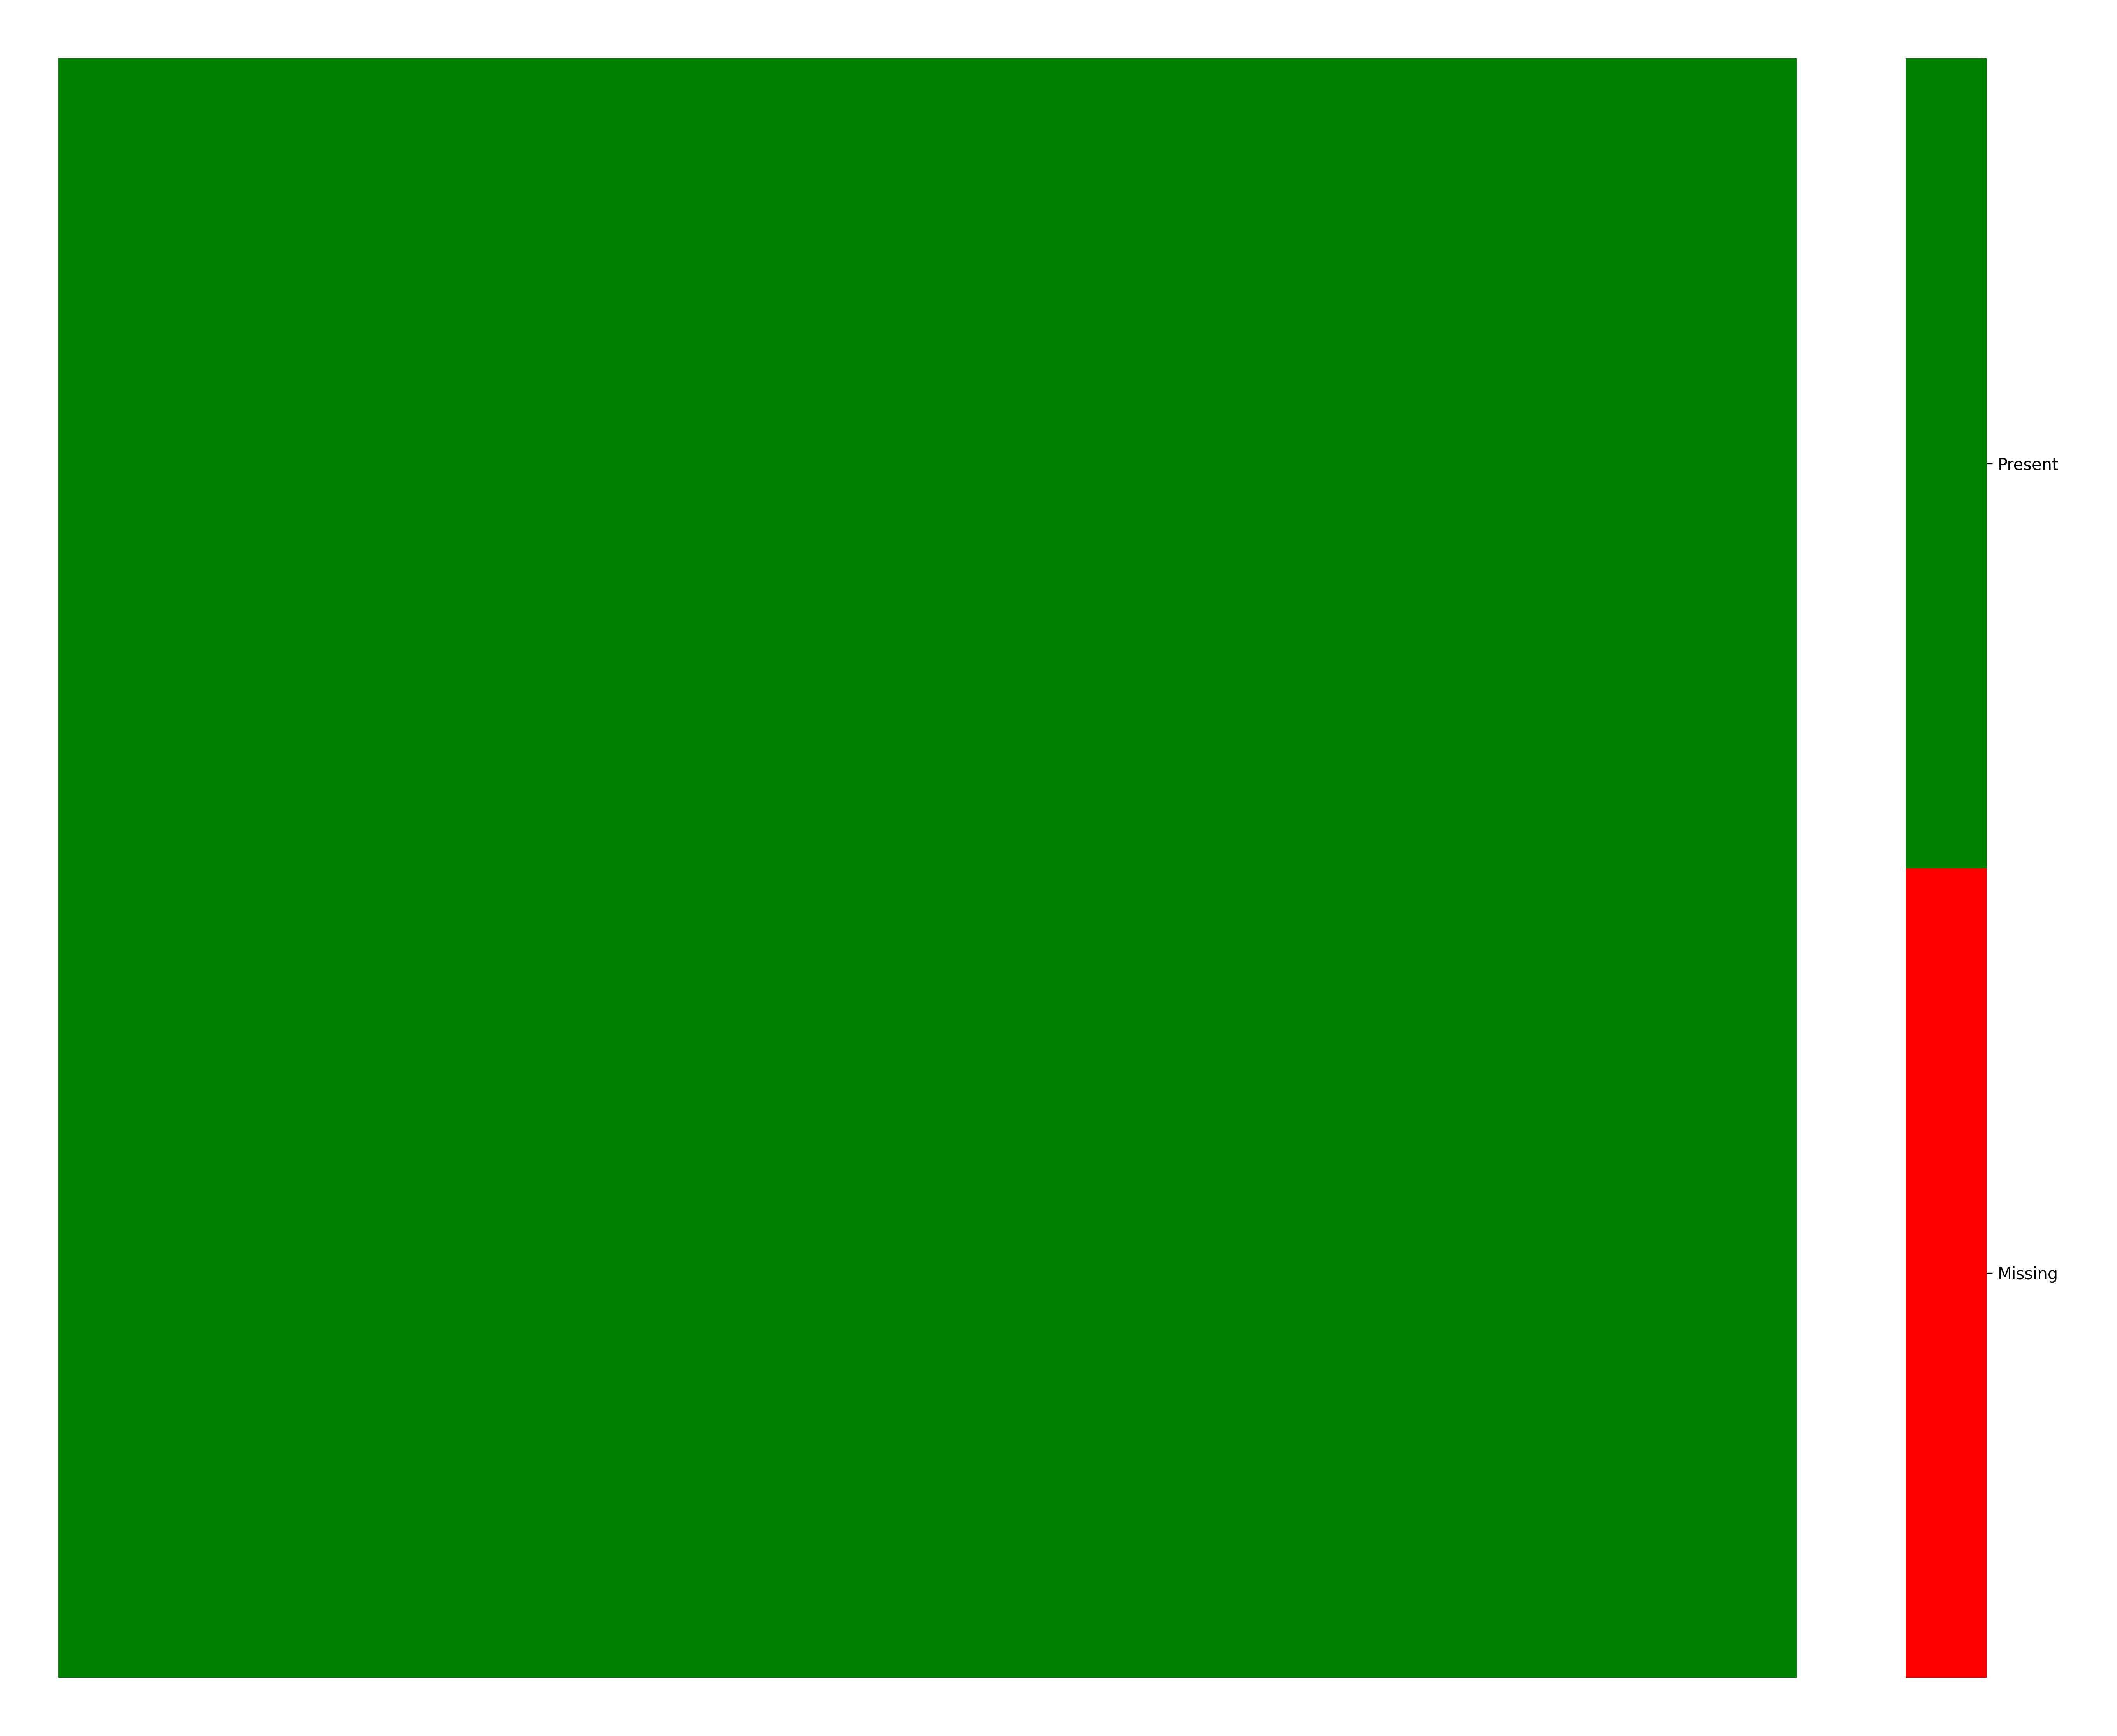
\includegraphics[width=\linewidth]{case9_bnb_heatmap_cleaned.png}
        \caption{BnB (Best)}
    \end{subfigure}
    \hfill
    \begin{subfigure}{0.45\textwidth}
        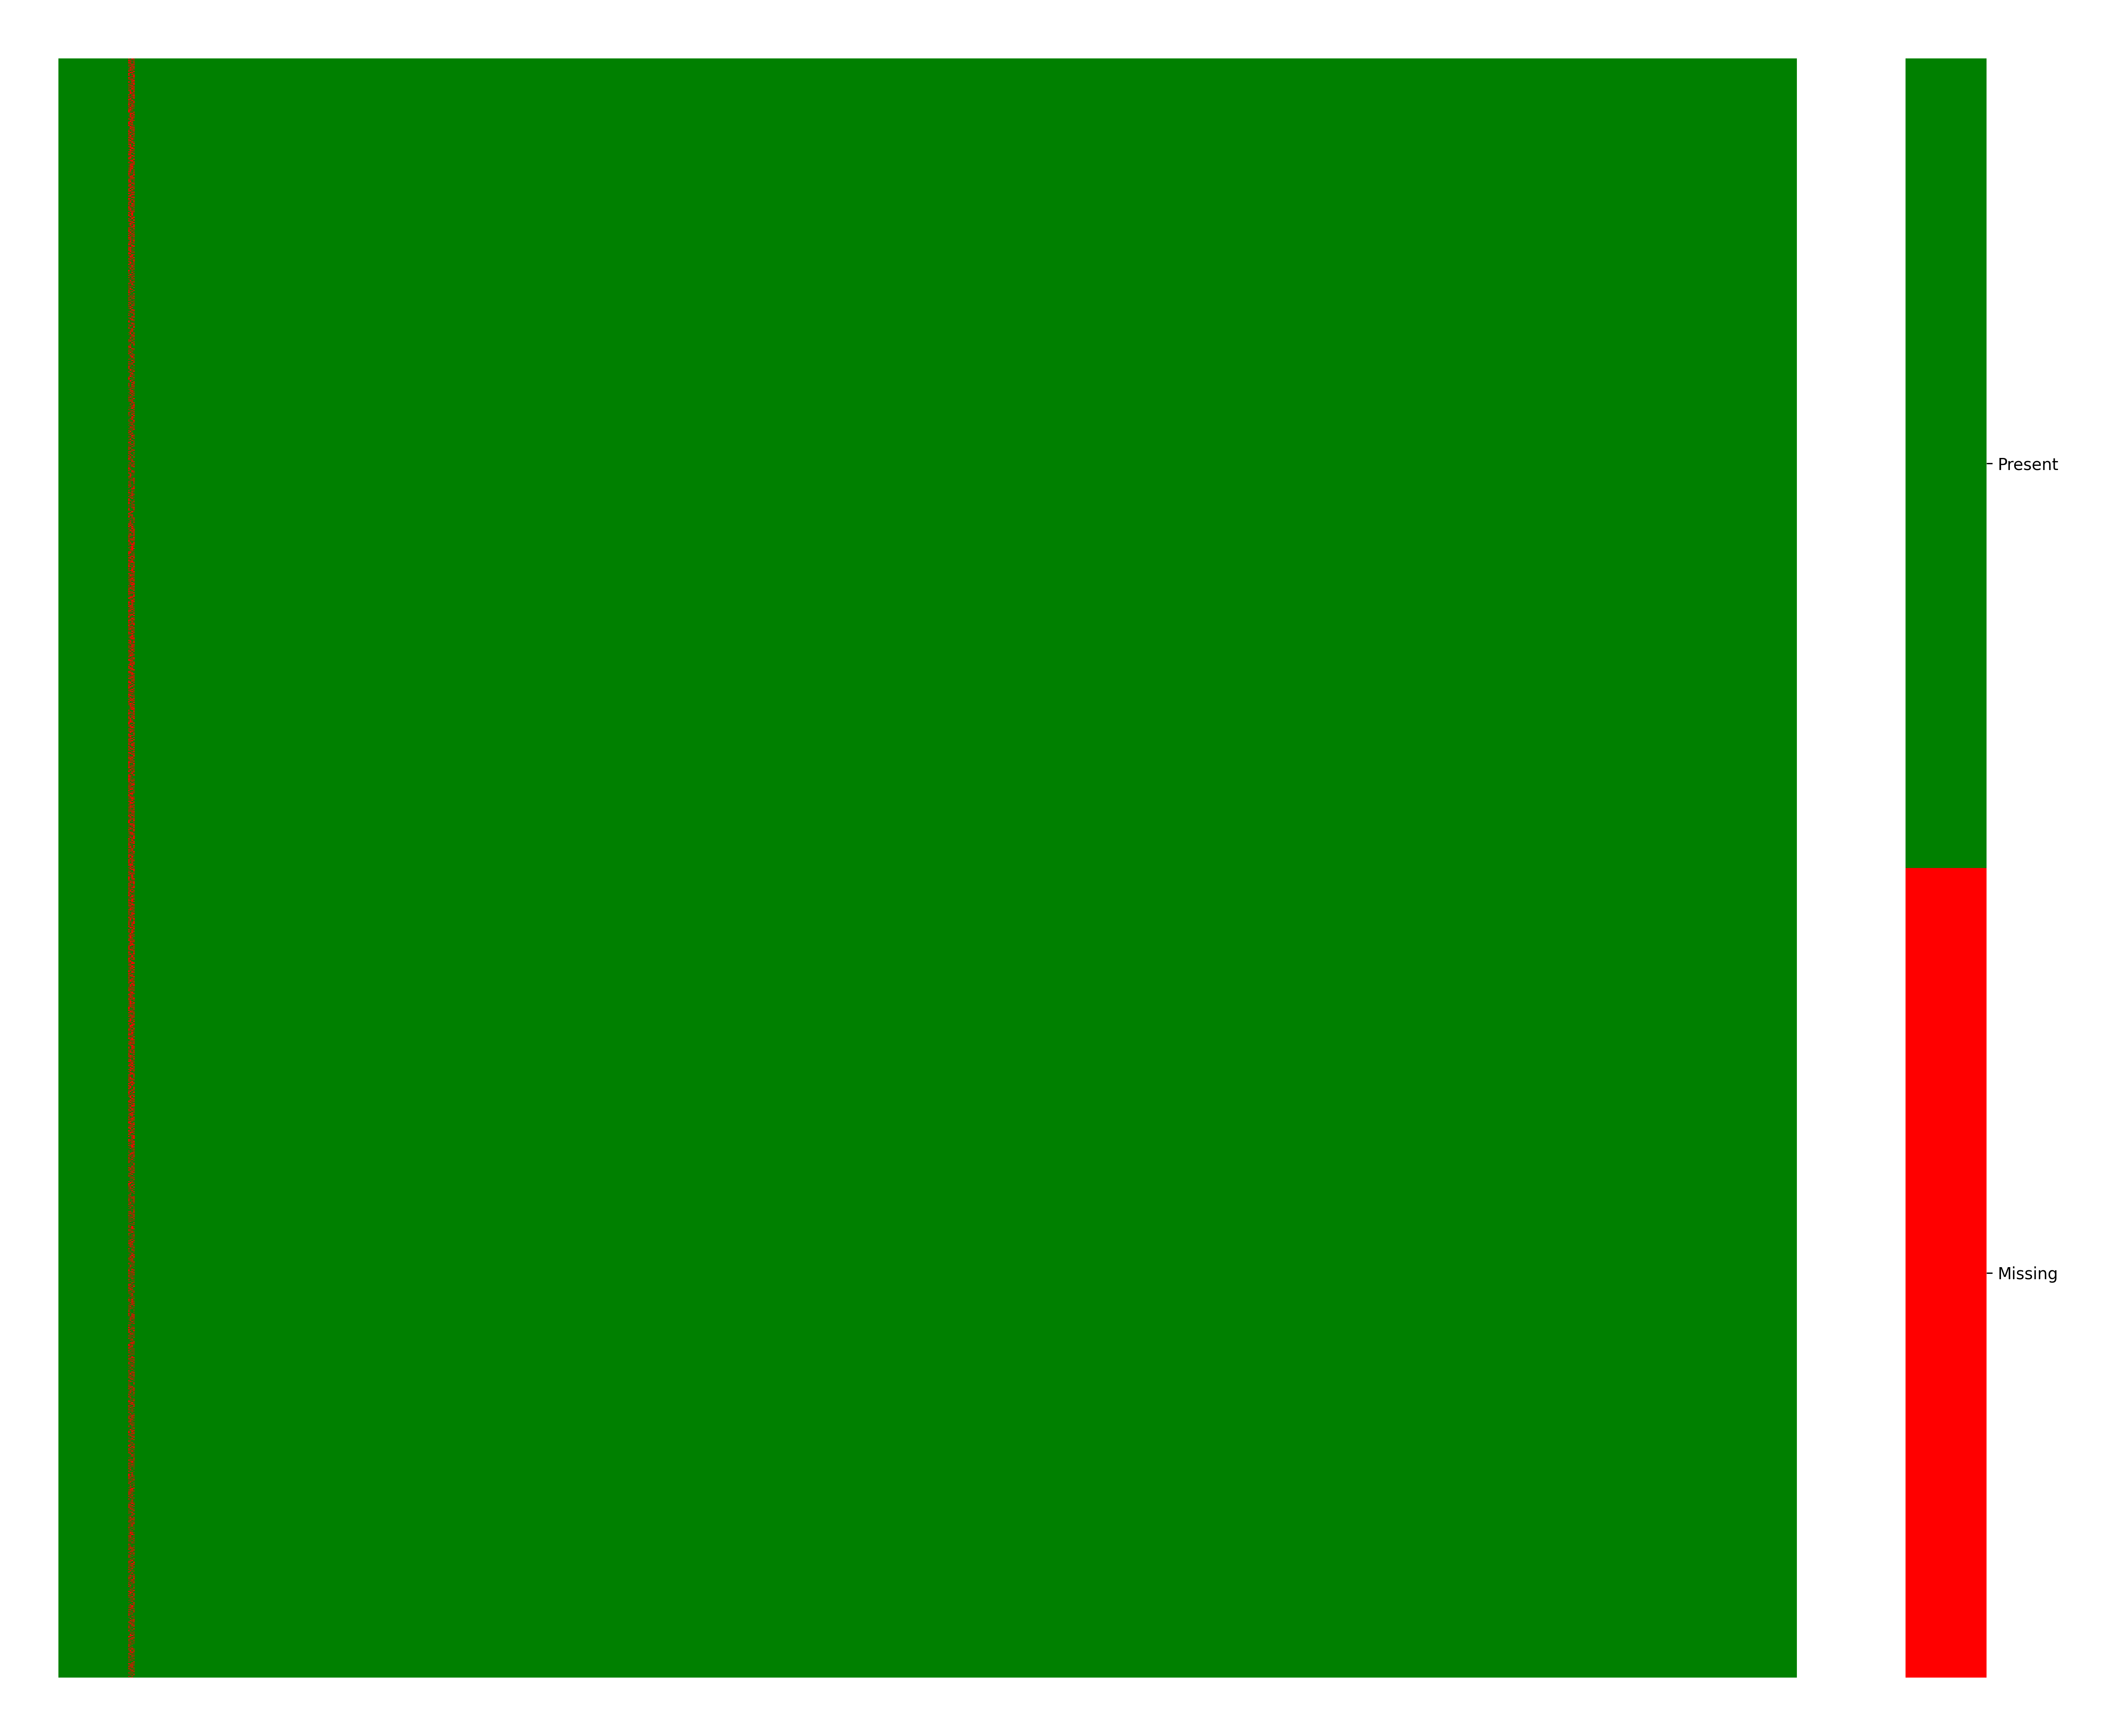
\includegraphics[width=\linewidth]{case9_v0.3_heatmap_cleaned.png}
        \caption{v0.3 (Worst)}
    \end{subfigure}
    \caption{Case 8 cleaned datasets comparison}
\end{figure}

\subsubsection{Case 9: MNAR – Complex Dependency}

\textbf{Score Table:}

\begin{table}[H]
\centering
\caption{Scores by algorithm, Case 9}
\label{tab:score_algorithms_case9}
\begin{tabular}{|c|c|c|c|c|c|c|c|c|}
\hline
Algorithm & v0.0 & v0.1 & v0.2 & v0.3 & v0.4 & v0.5 & BnB & Average \\
\hline
Score & 65.2 & 62.8 & 60.6 & 58.4 & 60.8 & 60.8 & 70.0 & \textbf{62.67}  \\
\hline
\end{tabular}
\end{table}

\textbf{Observations}\\
Again, BnB outperforms all other algorithms with a score of 70.0. It has perfect results in constraint adherence, retention, and bonus. The lowest score comes from v0.3 (58.4), with notably low adherence (32/40) and Data Retention (15.5/20). The performance gap is 11.6 points, again showing lower variance. 

\textbf{Heatmaps}\\
The input dataset reflects a typical MNAR pattern with missing values concentrated across specific columns.

\begin{figure}[H]
    \centering
    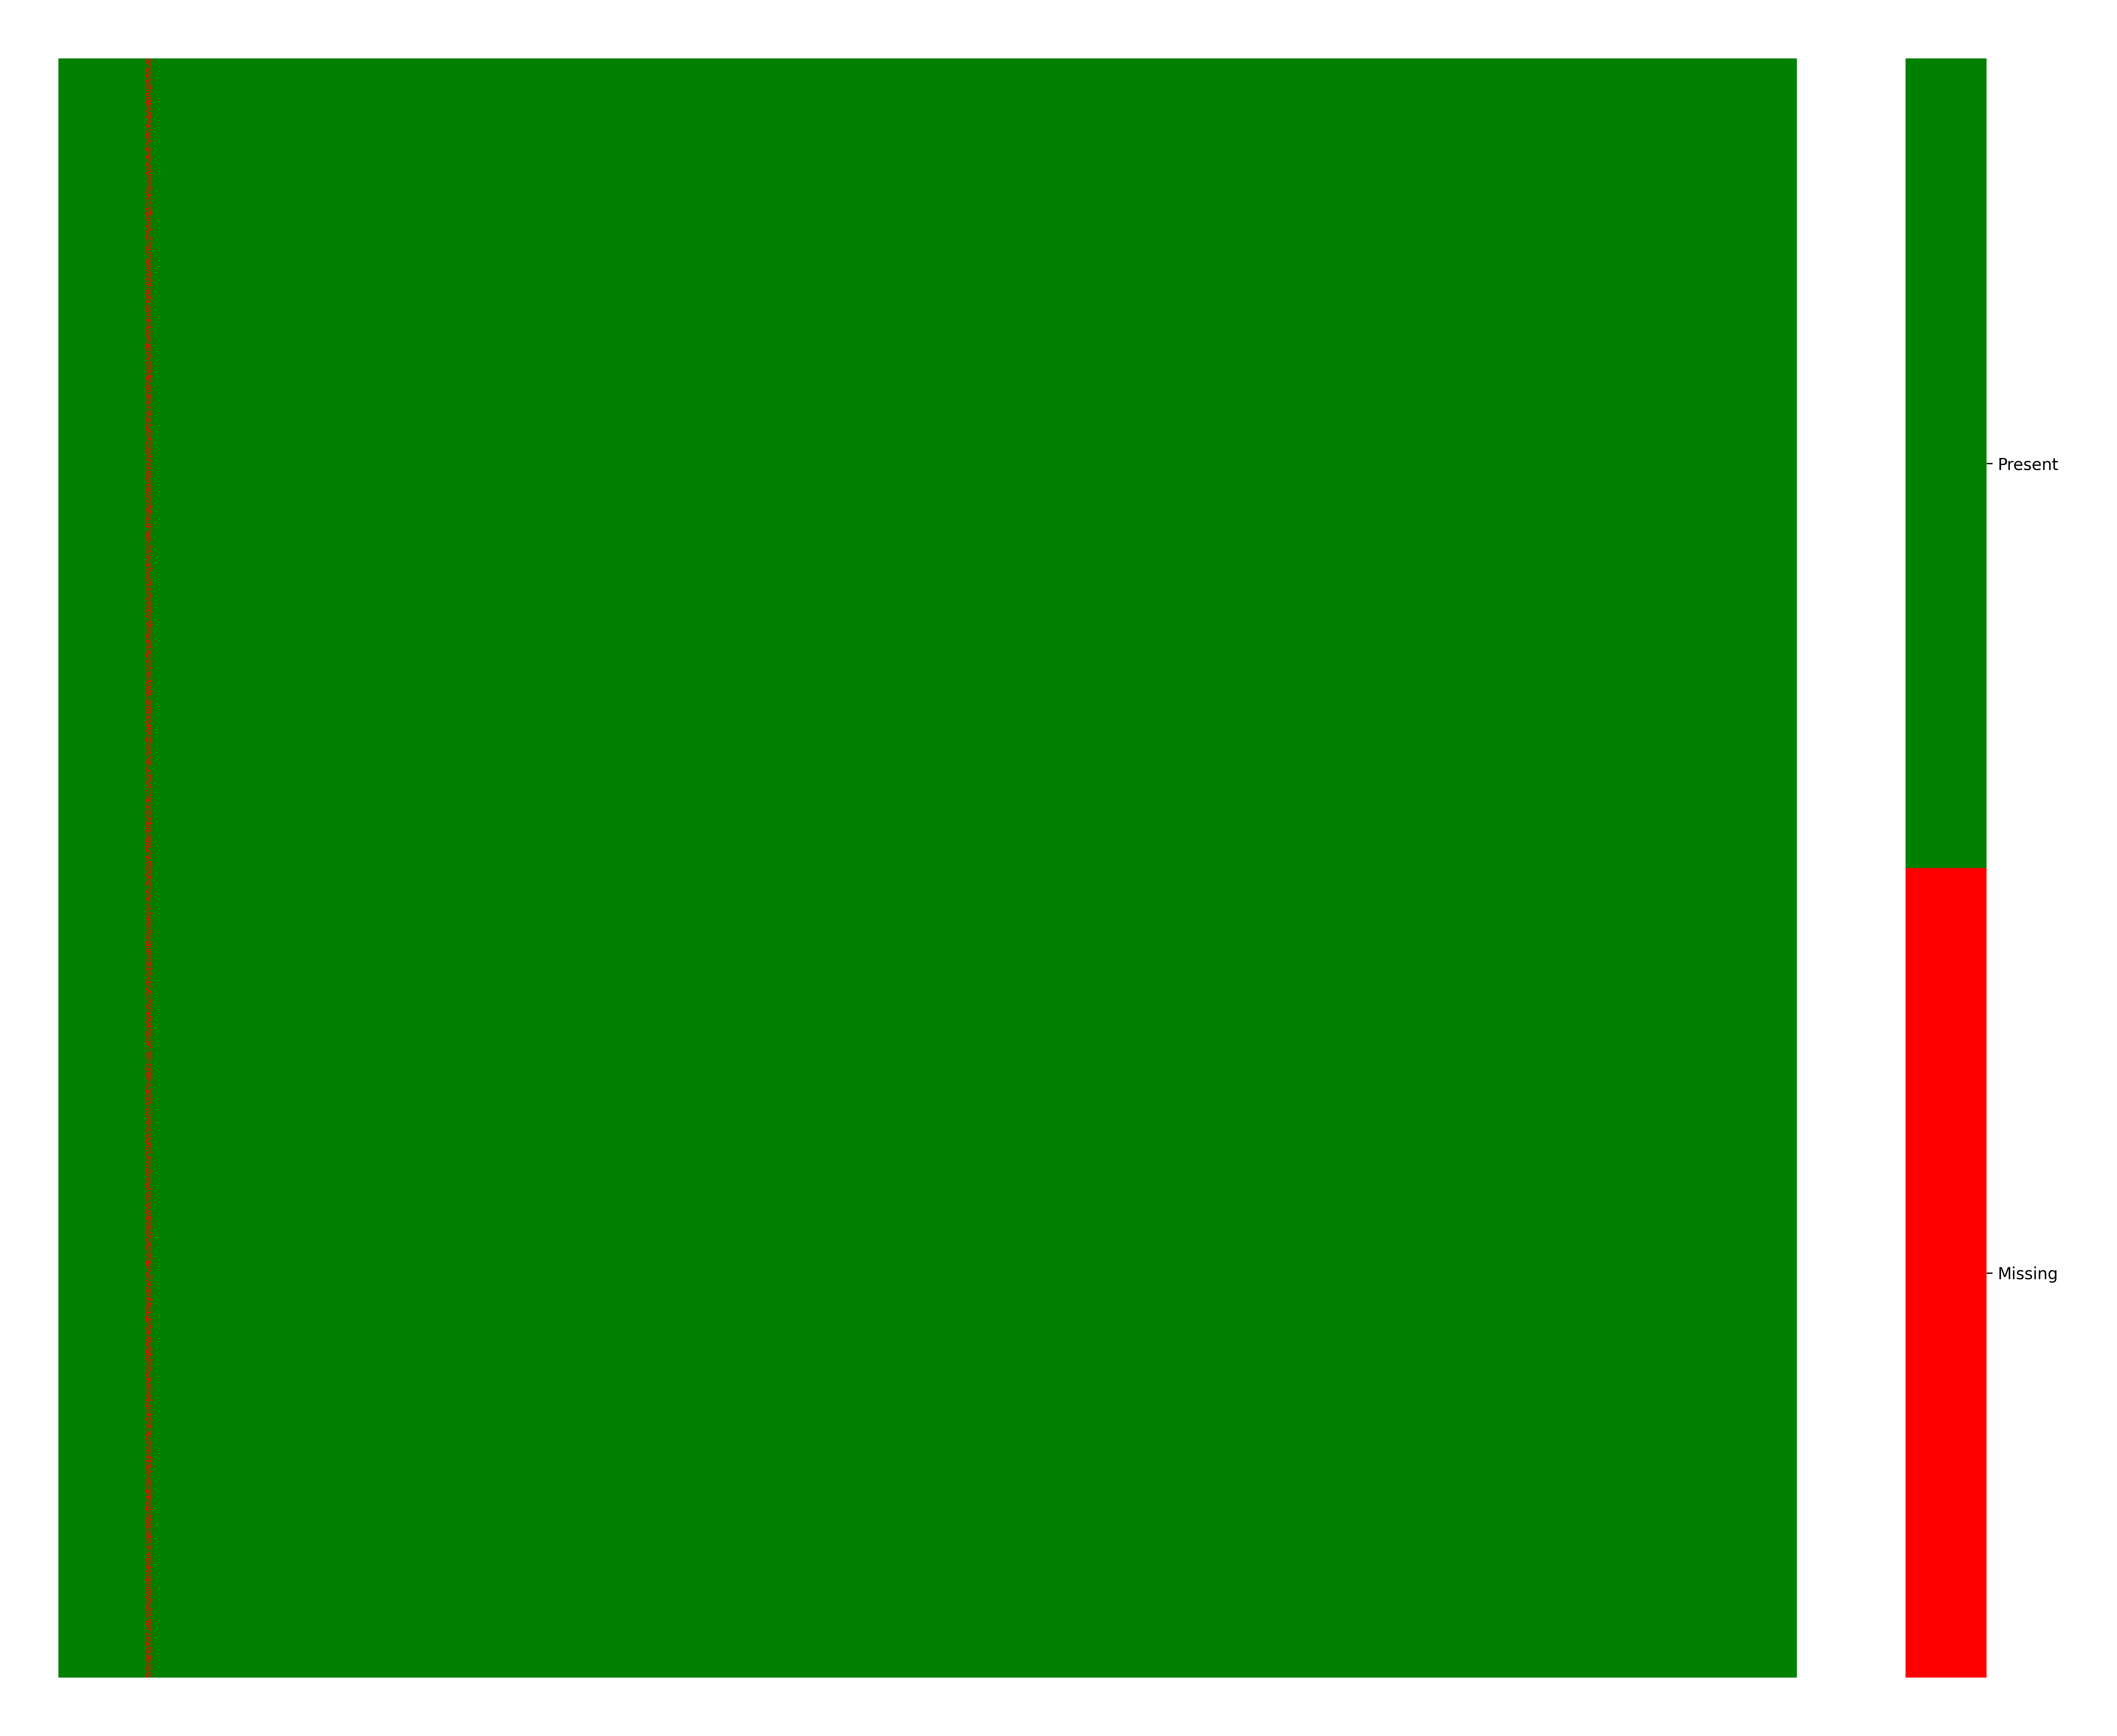
\includegraphics[width=0.5\linewidth]{case10_heatmap_erased.png}
    \caption{Case 9 Input Dataset}
\end{figure}

After applying BnB, important columns are filled, and the pattern remains visually consistent. In contrast, v0.3 shows broken column segments.

\begin{figure}[H]
    \centering
    \begin{subfigure}{0.45\textwidth}
        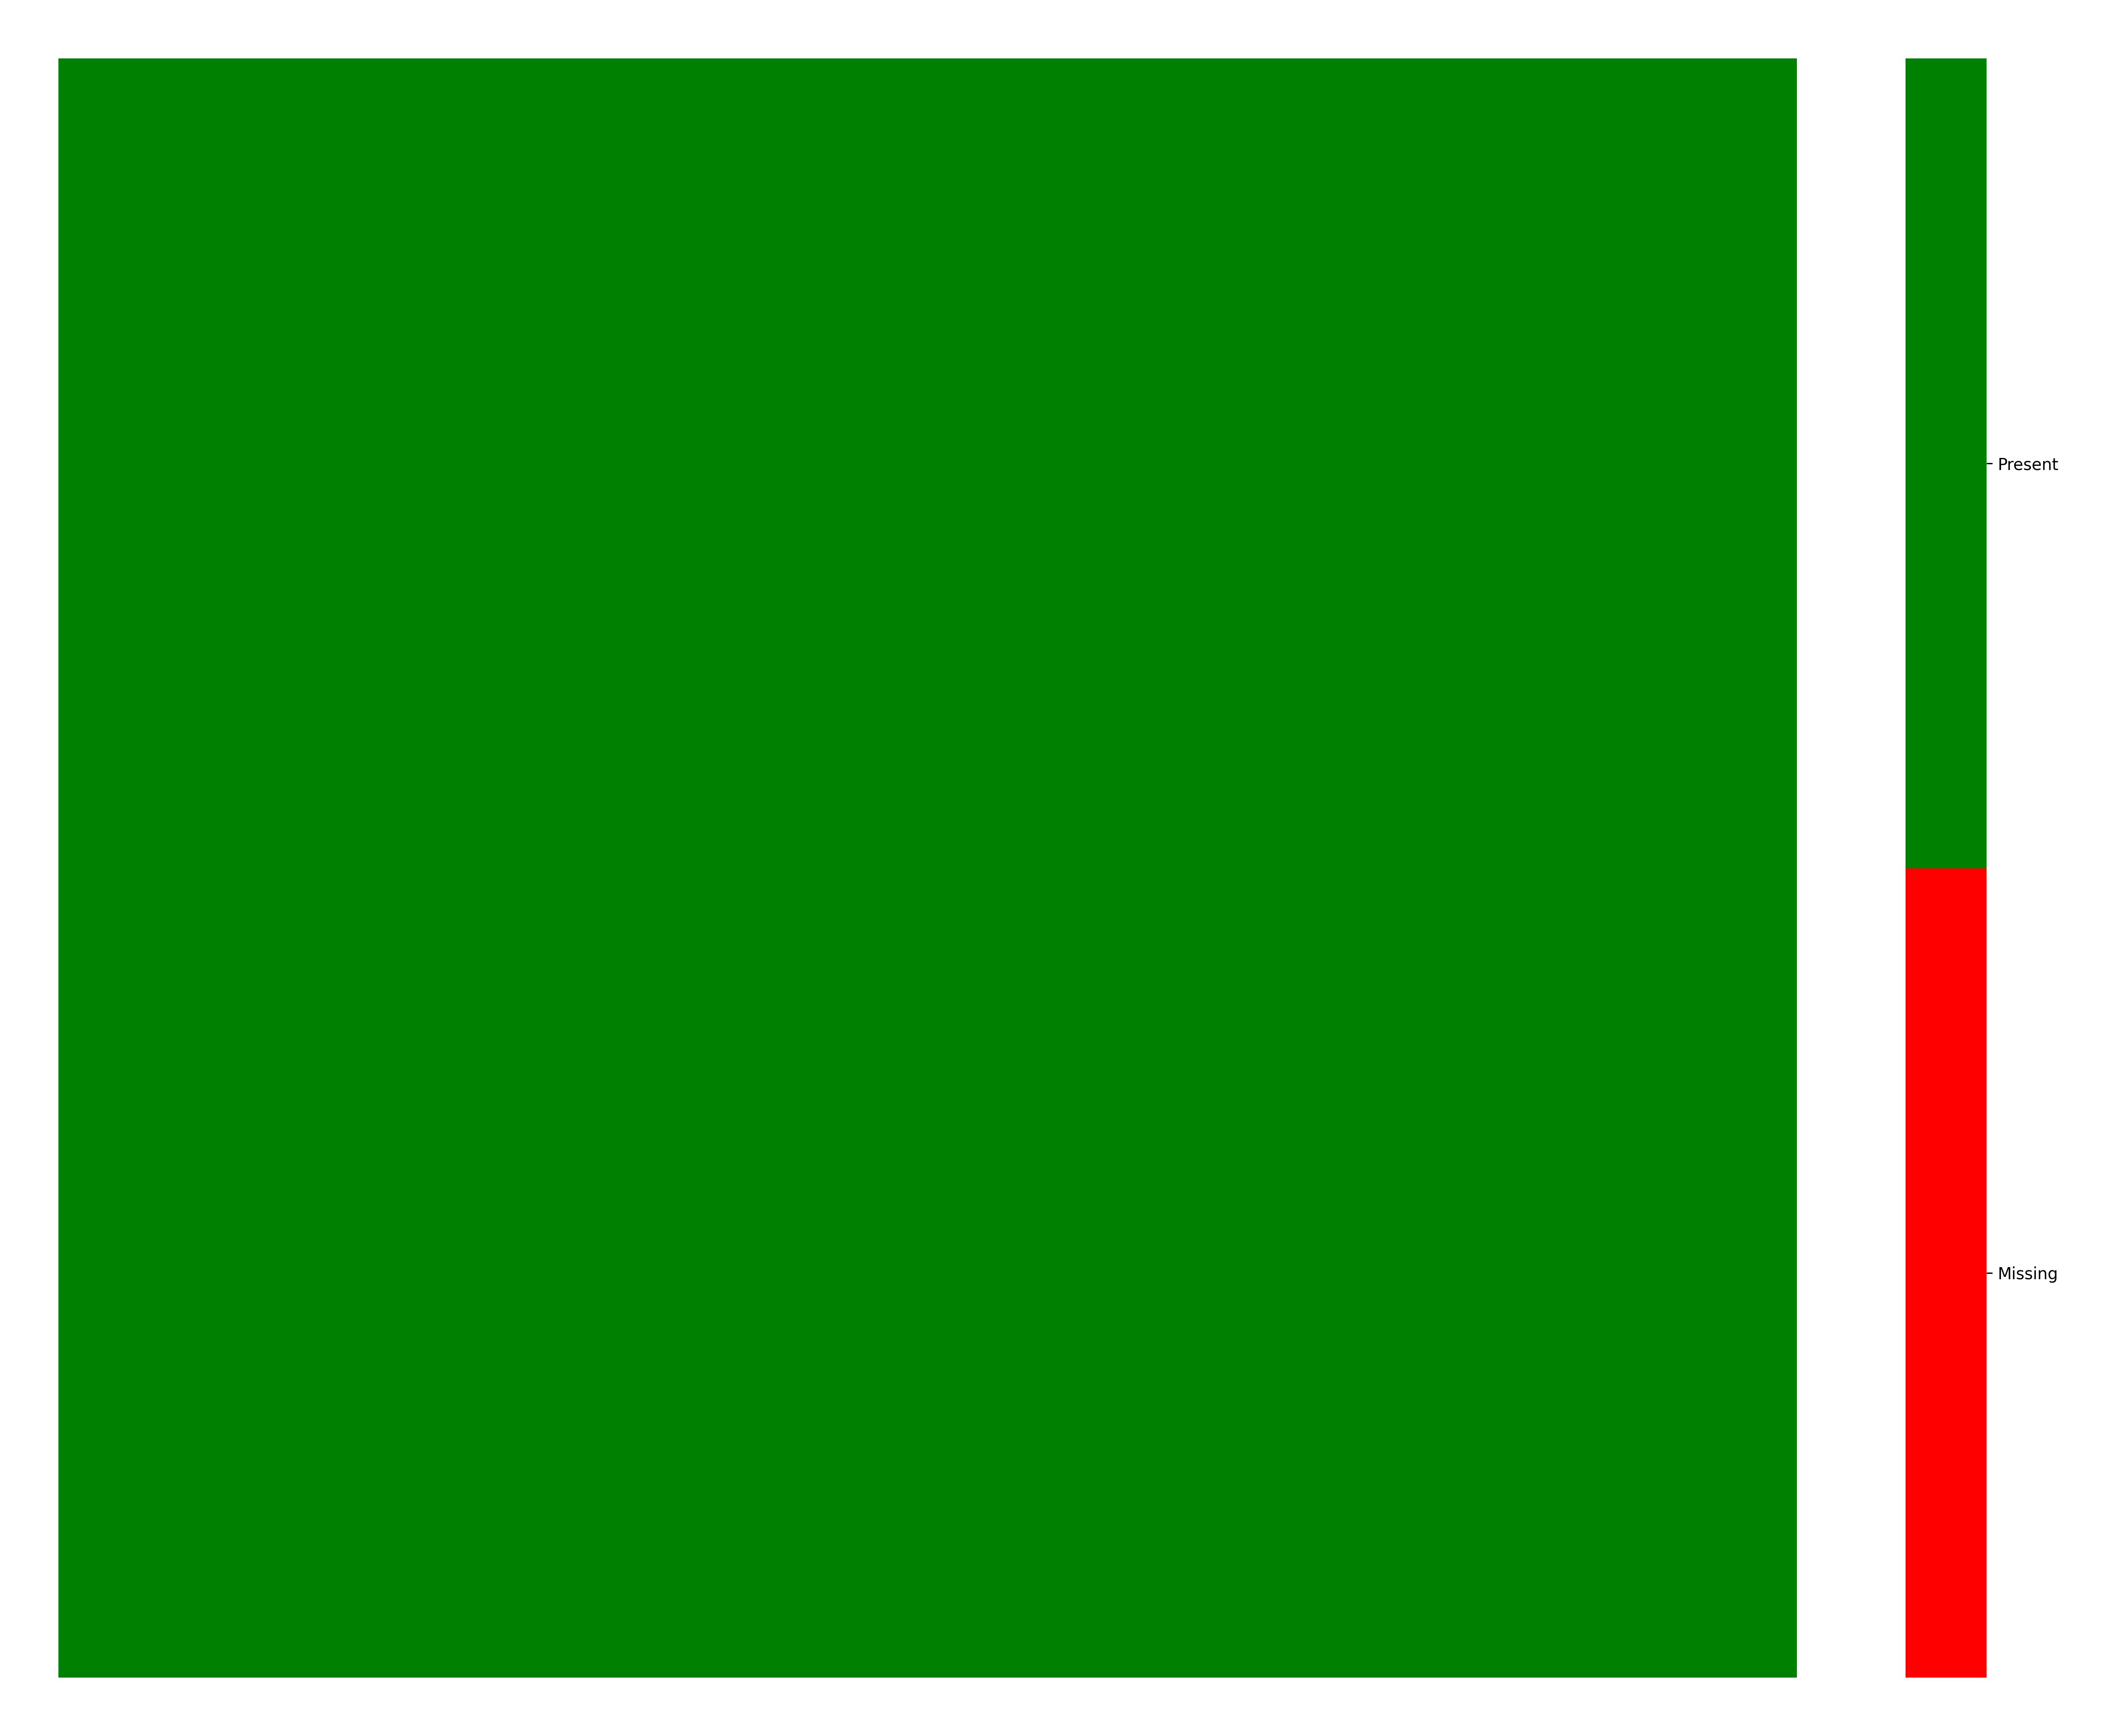
\includegraphics[width=\linewidth]{case10_bnb_heatmap_cleaned.png}
        \caption{BnB (Best)}
    \end{subfigure}
    \hfill
    \begin{subfigure}{0.45\textwidth}
        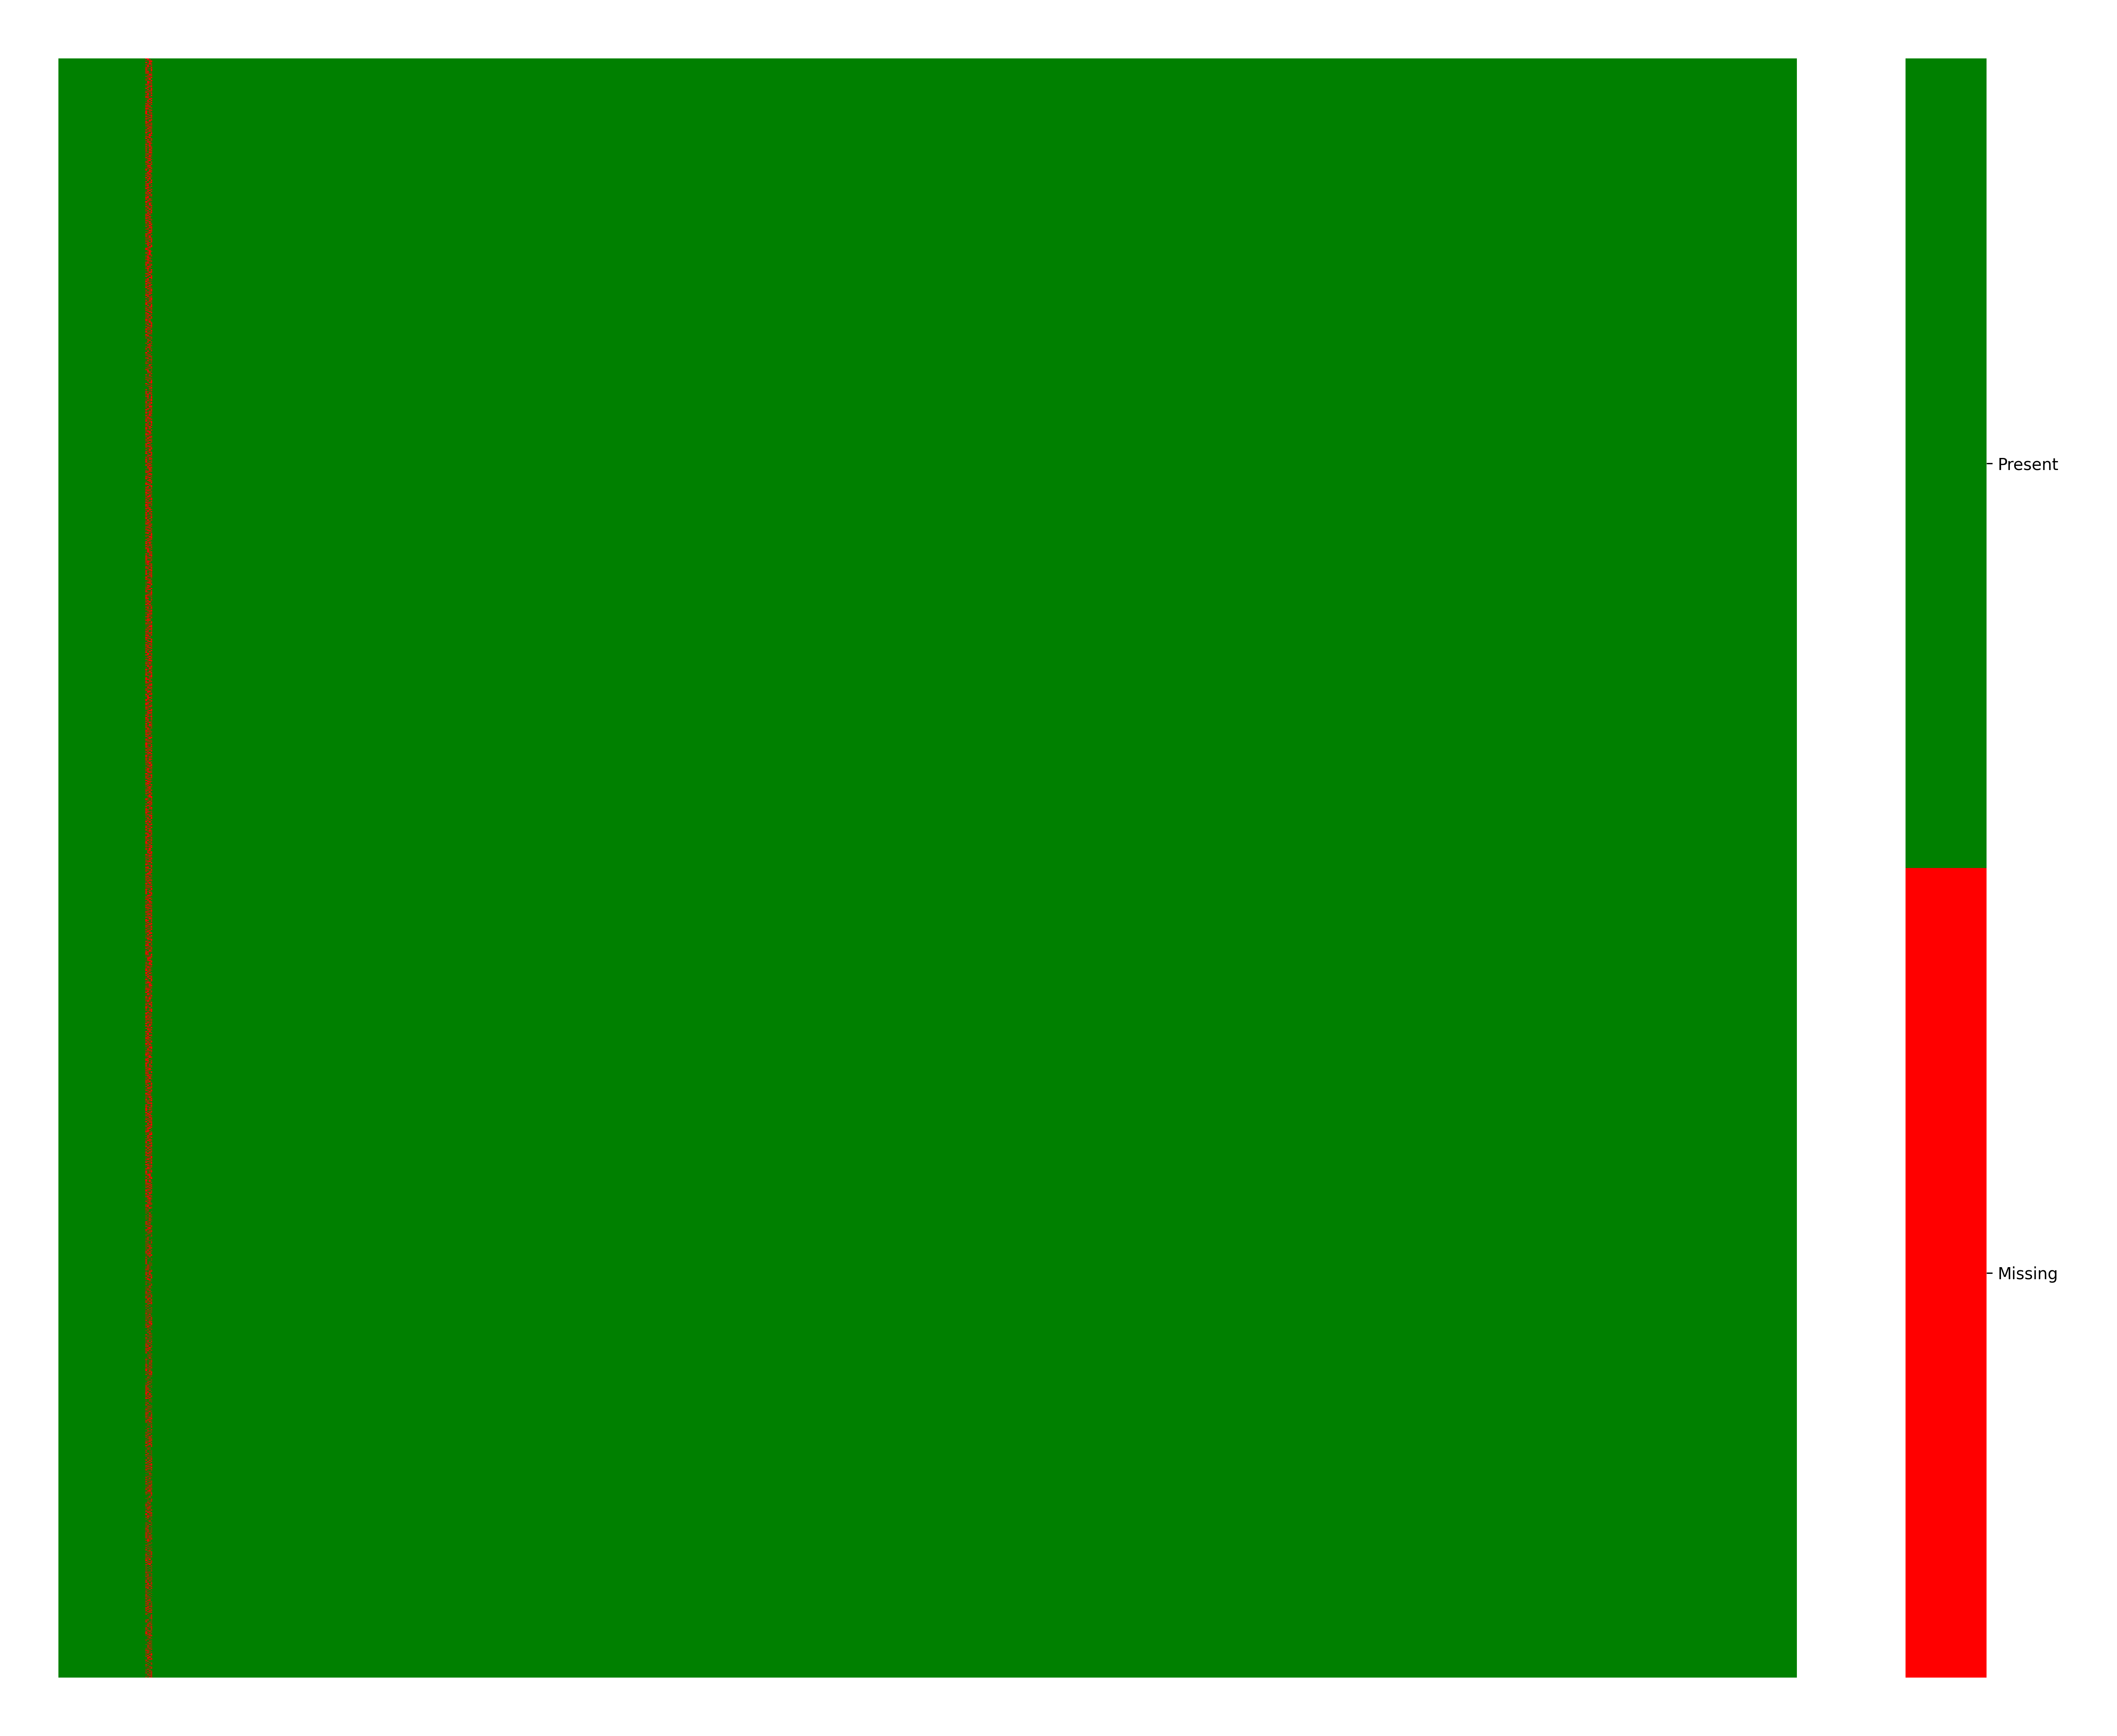
\includegraphics[width=\linewidth]{case10_v0.3_heatmap_cleaned.png}
        \caption{v0.3 (Worst)}
    \end{subfigure}
    \caption{Case 9 cleaned datasets comparison}
\end{figure}
\subsection{Results and Interpretation}
To understand the performance of each algorithm, we calculated the mean score across all test cases:  
\begin{itemize}
\item \textbf{v0.4:} 72.2
\item \textbf{v0.5:} 71.9
\item \textbf{BnB:} 68.0
\item \textbf{v0.0:} 64.1
\item \textbf{v0.1:} 61.0
\item \textbf{v0.2:} 60.7
\item \textbf{v0.3:} 58.1
\end{itemize}
These results demonstrate that \textbf{v0.4}, \textbf{v0.5}, and \textbf{BnB} achieve the best mean scores. 

\subsubsection{Algorithmic Observations}
\begin{itemize}
\item \textbf{BnB:}
\begin{itemize}
\item Best for complex MAR and MNAR patterns (Cases 4, 6, 8, 9).
\item Struggles with high-MCAR scenarios (e.g., Case 2, Score: 52.0).
\end{itemize}
\item \textbf{v0.4 / v0.5:}
\begin{itemize}
\item Top performers in high-MCAR cases.
\item Underperform in MAR and MNAR scenarios.
\end{itemize}
\item \textbf{v0.0:}
\begin{itemize}
\item Effective in low-to-moderate complexity cases.
\item Struggles with complex dependencies.
\end{itemize}
\item \textbf{v0.3:}
\begin{itemize}
\item Worst average performance.
\end{itemize}
\end{itemize}

\paragraph{Variance}
Result variance is highest in MCAR scenarios and lower for MAR and MNAR. This occurs because MCAR's uniform randomness allows algorithms to respond divergently - some impute aggressively while others conservatively. In contrast, MAR and MNAR's structured dependencies constrain algorithmic behavior, yielding more consistent outcomes across methods.
\begin{landscape}
\begin{figure}[H]
\centering
\resizebox{0.9\textheight}{!}{ % Better scaling for landscape
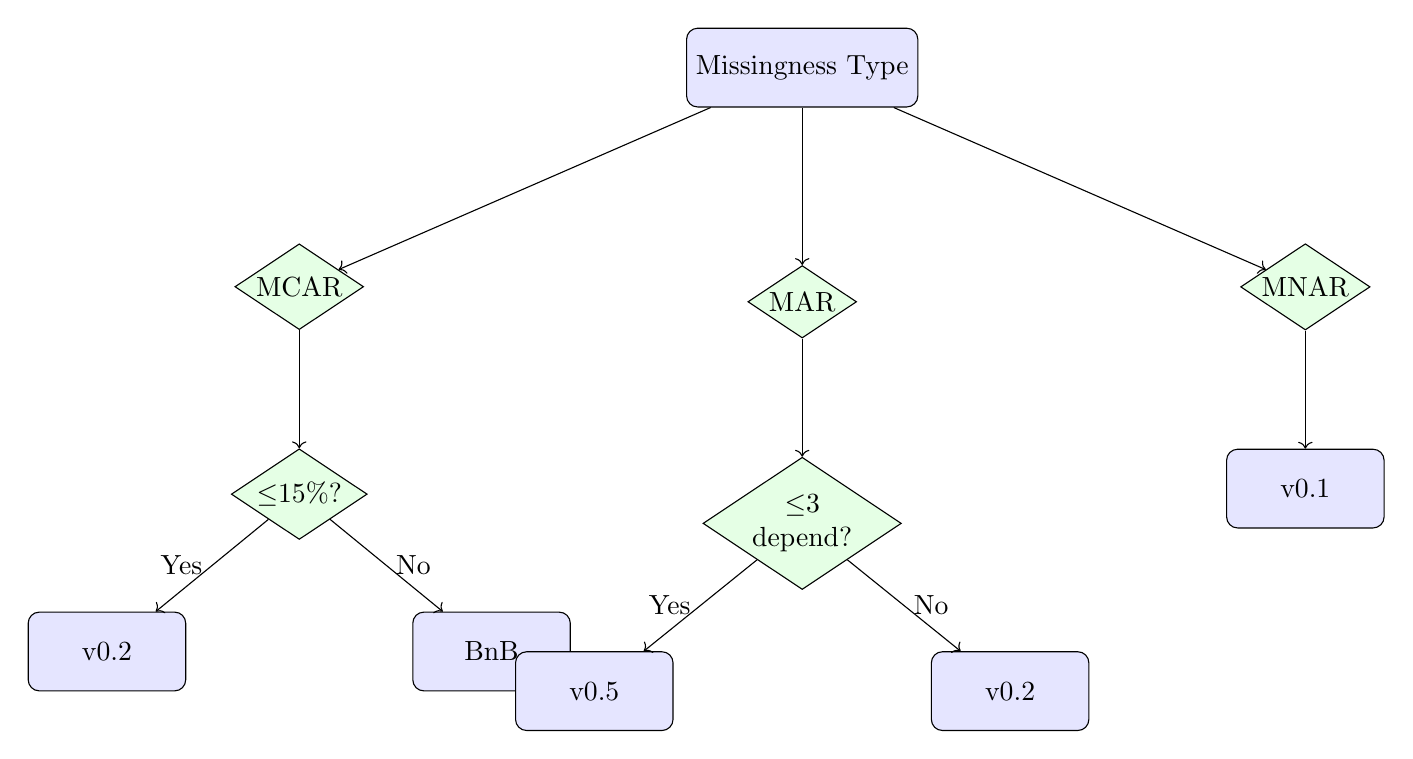
\begin{tikzpicture}[
    node distance=1.2cm and 2.5cm, % Reduced vertical spacing
    every node/.style={align=center},
    block/.style={rectangle, draw, fill=blue!10, rounded corners, minimum width=2cm, minimum height=1cm},
    decision/.style={diamond, draw, fill=green!10, aspect=1.5, inner sep=1pt}
]

% Main node
\node [block] (A) {Missingness Type};

% Balanced horizontal spacing
\node [decision, below left=2cm and 4.5cm of A] (B) {MCAR}; % Reduced horizontal offset
\node [decision, below=2cm of A] (E) {MAR};
\node [decision, below right=2cm and 4.5cm of A] (H) {MNAR}; % Reduced horizontal offset

% Diagonal connections
\draw [->] (A) -- (B);
\draw [->] (A) -- (E);
\draw [->] (A) -- (H);

% MCAR branch
\node [decision, below=1.5cm of B] (B1) {$\leq$15\%?};
\node [block, below left=1.2cm and 1cm of B1] (C) {v0.2};
\node [block, below right=1.2cm and 1cm of B1] (D) {BnB};
\draw [->] (B) -- (B1);
\draw [->] (B1) -- node[midway,left] {Yes} (C);
\draw [->] (B1) -- node[midway,right] {No} (D);

% MAR branch
\node [decision, below=1.5cm of E] (E1) {$\leq$3 \\ depend?};
\node [block, below left=1.2cm and 1cm of E1] (F) {v0.5};
\node [block, below right=1.2cm and 1cm of E1] (G) {v0.2};
\draw [->] (E) -- (E1);
\draw [->] (E1) -- node[midway,left] {Yes} (F);
\draw [->] (E1) -- node[midway,right] {No} (G);

% MNAR branch
\node [block, below=1.5cm of H] (I) {v0.1};
\draw [->] (H) -- (I);

\end{tikzpicture}
}
\caption{Algorithm selection flowchart based on missingness characteristics}
\label{fig:flowchart}
\end{figure}
\end{landscape}

\subsection{Real World Application}
To validate the behavior of the algorithms in a more practical and realistic scenario, we applied them to a real-world dataset containing missing values. This phase of the experimentation aims to assess whether the patterns observed in the synthetic data persist when applied to real data.

\subsubsection{Real Dataset}
The set of real data used comes from a practical exercise obtained from a medical questionnaire used in a data mining subject. The missing pattern was not controlled, and therefore, you can't clearly classify it as MCAR, MAR or MNAR. However, using a visual analysis it was detected dependencies that suggest a mix of MNAR and MAR. 

\subsubsection{Analysis}
Here we are only going to compare the two best obtained results: v0.3, v0.2 and v0.5. We are going to compare the clustering structure and the silhouette score.
\begin{itemize}
    \item Version \textbf{v0.3} achieved the best result in terms of average silhouette score ($\approx 0.52$), giving us clear and consistent segmentation between groups. This can be seen in the clustering heatmaps, where the reconstruction showed clean blocks and smooth transitions between regions.
    \item Version \textbf{v0.2} also reached an acceptable silhouette score ($\approx 0.48$), supporting its ability to preserve latent relationships despite employing a simpler logic.
    \item Version \textbf{v0.5}, despite its more aggressive approach and strong metric performance, underperformed when compared to the others, with a silhouette score of ($\approx 0.39$). This suggests that the aggressiveness of the algorithm is negatively impacting the formation of distinct clusters.
\end{itemize}

\begin{figure}[H]
\centering
\begin{subfigure}{0.48\textwidth}
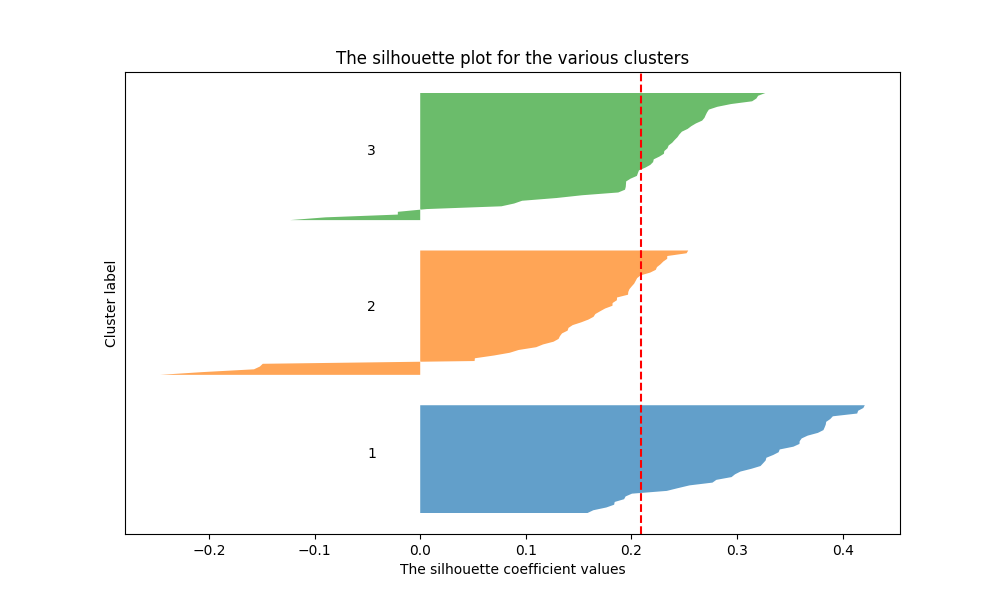
\includegraphics[width=\linewidth]{results_silhouette_og.png}
\caption{Original}
\end{subfigure}
\hfill
\begin{subfigure}{0.48\textwidth}
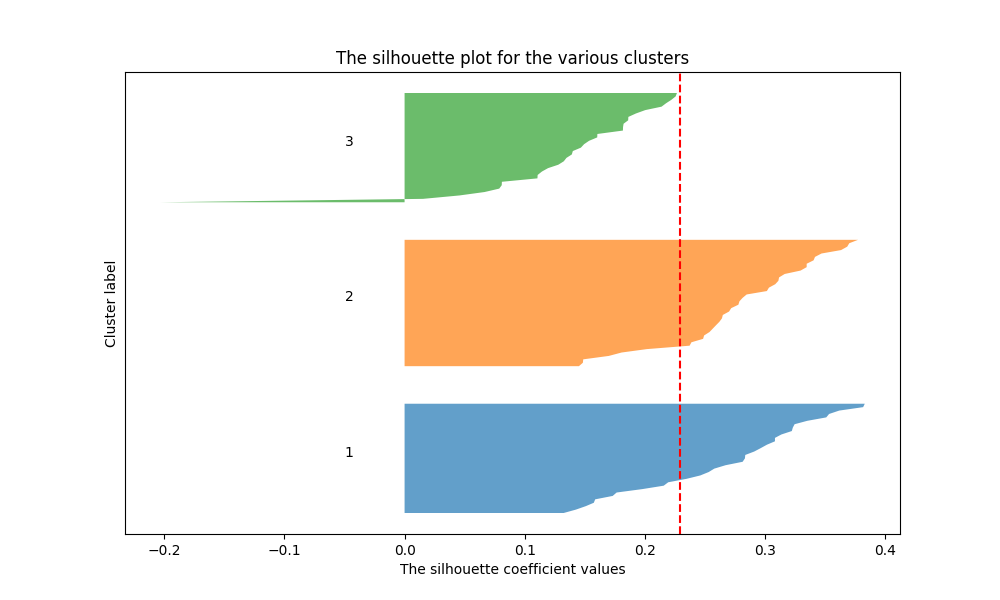
\includegraphics[width=\linewidth]{results_silhouette_v3.png}
\caption{v0.3}
\end{subfigure}
\caption{Original and v0.3 (silhouette)}
\end{figure}

\begin{figure}[H]
\centering
\begin{subfigure}{0.48\textwidth}
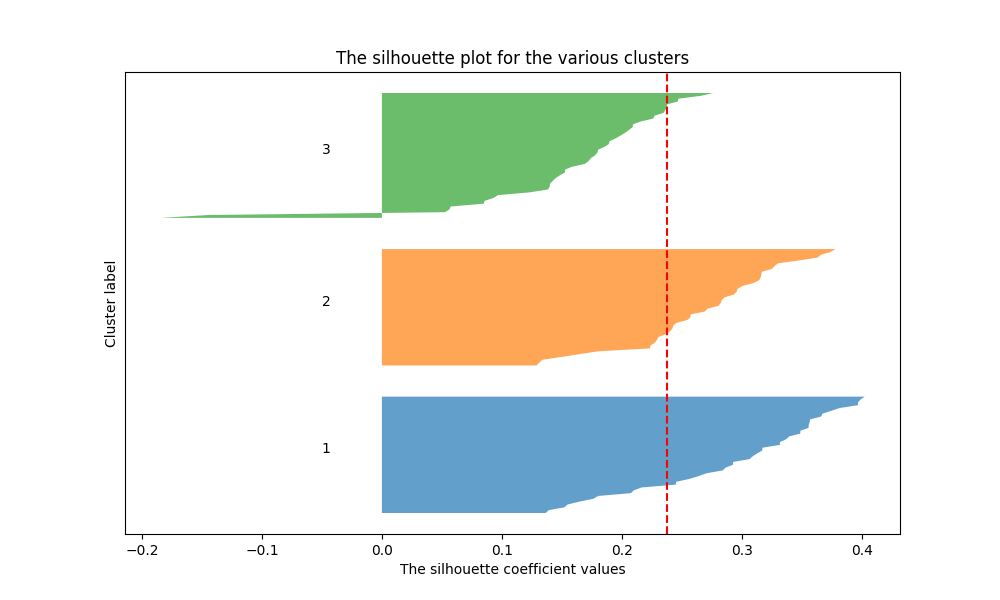
\includegraphics[width=\linewidth]{results_silhouette_v2.png}
\caption{v0.2}
\end{subfigure}
\hfill
\begin{subfigure}{0.48\textwidth}
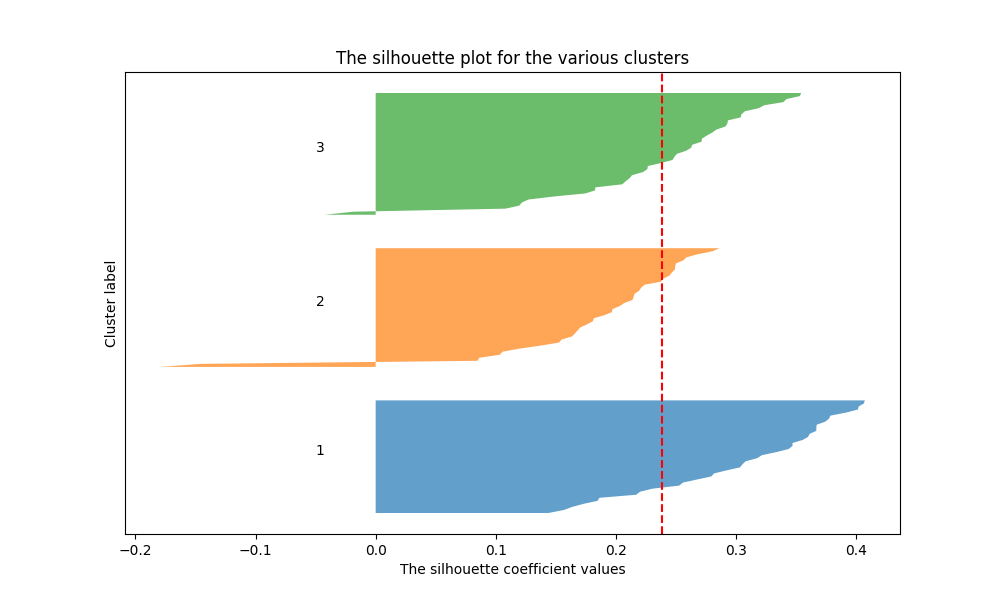
\includegraphics[width=\linewidth]{results_silhouette_v0_5.png}
\caption{v0.5}
\end{subfigure}
\caption{v0.2 and v0.5 (silhouette)}
\end{figure}

\begin{figure}[H]
\centering
\begin{subfigure}{0.48\textwidth}
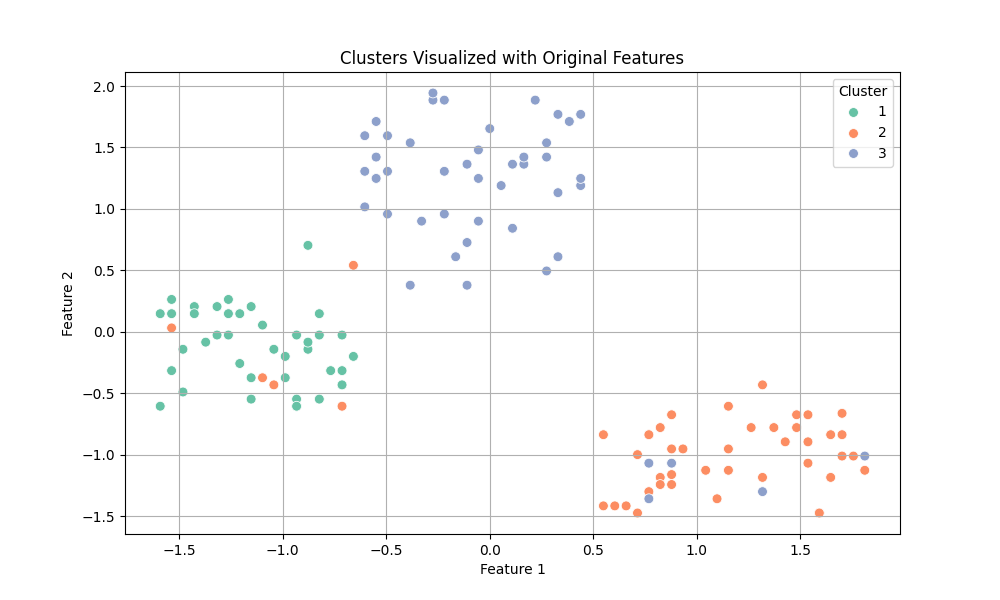
\includegraphics[width=\linewidth]{results_Cluster_og.png}
\caption{Original}
\end{subfigure}
\hfill
\begin{subfigure}{0.48\textwidth}
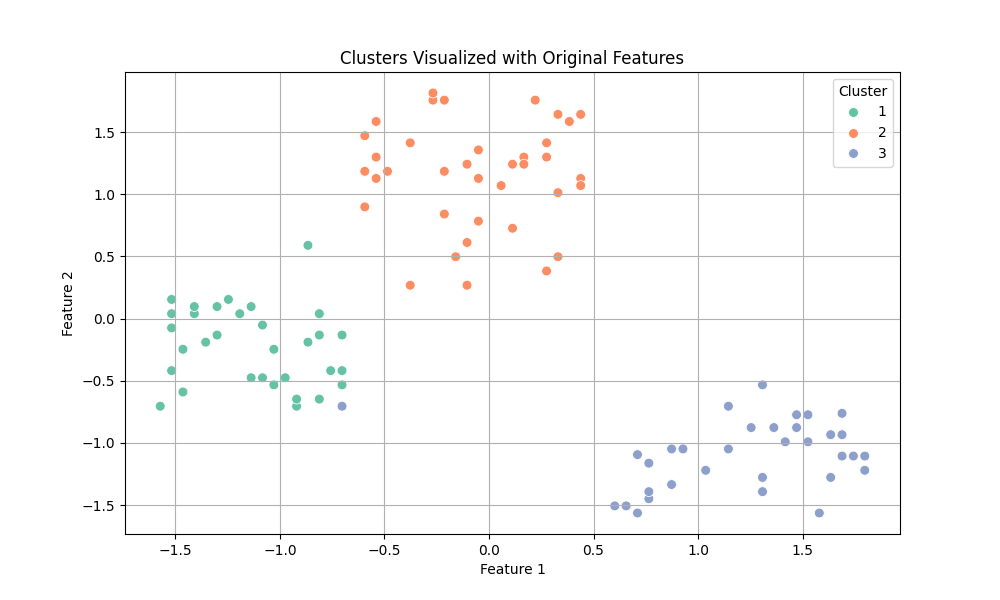
\includegraphics[width=\linewidth]{results_Cluster_v3.png}
\caption{v0.3}
\end{subfigure}
\caption{Original and v0.3 (clustering)}
\end{figure}

\begin{figure}[H]
\centering
\begin{subfigure}{0.48\textwidth}
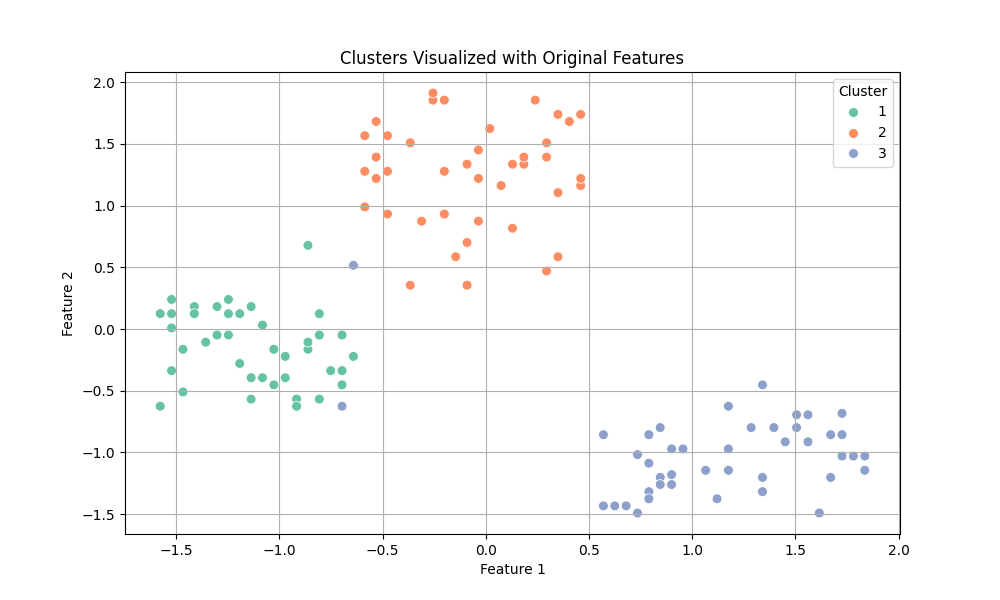
\includegraphics[width=\linewidth]{results_Cluster_v2.png}
\caption{v0.2}
\end{subfigure}
\hfill
\begin{subfigure}{0.48\textwidth}
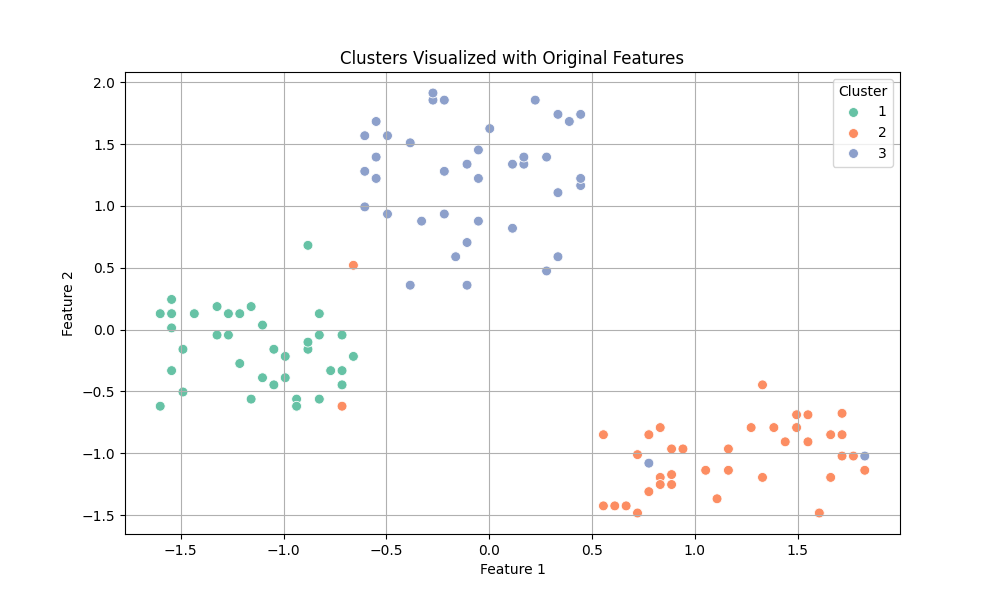
\includegraphics[width=\linewidth]{results_Cluster_v0_5.png}
\caption{v0.5}
\end{subfigure}
\caption{v0.2 and v0.5 (clustering)}
\end{figure}

\subsubsection{Interpretation}

The silhouette index results match with the visual findings from the heatmaps. From there, we can conclude:

\begin{itemize}
    \item Simpler strategies, such as \textbf{v0.2} and \textbf{v0.3}, managed to preserve the dataset's latent structure.
    
    \item More aggressive approaches (e.g., \textbf{v0.5}, \textbf{BnB}), while improving data completeness, may come at the cost of reduced clustering capability.
\end{itemize}

\subsection{Limitations}
Despite the promising results obtained during experimentation, this work presents several limitations that should be taken into account to understand the final section.

\begin{itemize}
    \item \textbf{Dependence on Simulation:} Although the synthetic cases cover a wide range of scenarios (MCAR, MAR, MNAR), there is always a risk that simulations may not accurately reflect the complexity of real-world missing data patterns.

    \item \textbf{Evaluation Focused on Quantitative Score:} The \textit{health score} metric aggregates multiple evaluation criteria (constraints, completeness, retention, and important columns), but may obscure undesired trade-offs. For instance, an algorithm might retain fewer missing values by removing too many rows and still achieve a high overall score.

    \item \textbf{Computational Cost Not Included in Scoring:} Algorithms such as BnB exhibit significantly higher runtime compared to greedy methods, yet this dimension was not explicitly quantified in the scoring system. In real-world contexts where efficiency is critical, this factor may impact their applicability.

    \item \textbf{Trade-off Between Retention and Reconstruction:} Some algorithms, such as \textbf{v0.1}, tend to discard more data in order to obtain a more "complete" dataset. However, this can harm the underlying structure. This trade-off between completeness and structure preservation is not always clearly optimized.

    \item \textbf{Graphical Interface Not Empirically Evaluated:} Although a graphical interface was developed using \texttt{Tkinter}, its usability and effectiveness were not empirically evaluated with real users.
\end{itemize}
\newpage
\section{Conclusions and Future Work}
This project has demonstrated that it is possible to design and implement efficient strategies for handling missing values in high-dimensional datasets.

In particular, the following conclusions can be drawn:
\begin{itemize}
    \item Simple methods like \texttt{v0.0} perform competitively in MNAR scenarios. However, in MCAR, more sophisticated algorithms such as \texttt{v0.4}, \texttt{v0.5} achieve better performance.
    \item 
    \item The nature of the missing data mechanism (MCAR, MAR, or MNAR) significantly influences algorithm behavior. This underlines the importance of tailoring data cleaning strategies to the specific type of missingness present in the dataset.
    
    \item The evaluation metrics defined in this project (such as the \textit{health score}) enable objective and reproducible comparisons, providing practical guidance for selecting the most suitable imputation or deletion strategy.
    
    \item The application of the algorithms to a real-world dataset validated the approach in an uncontrolled environment. The results indicated that simpler methods preserve tend to produce more coherent clustering outcomes.
\end{itemize}

\subsection{Summary of Achievements}
This project has successfully fulfilled its initial objectives, both theoretical and practical.

\subsubsection{Theoretical Contributions}
\begin{itemize}
    \item Analyzed the different types of missing data: MCAR (Missing Completely At Random), MAR (Missing At Random), and MNAR (Missing Not At Random).
    
    \item Investigated the impact of missing values on clustering quality, with effects quantified using metrics such as the silhouette index and cluster heatmaps.
    
    \item Designed a reproducible evaluation framework for comparing algorithmic performance. This framework integrates user-defined constraints, missing value reduction, data retention, and the preservation of key variables.
\end{itemize}

\subsubsection{Practical Contributions}
\begin{itemize}
    \item Developed multiple algorithms based on different heuristics. The implementation of the Branch and Bound method enabled direct comparison between greedy and exhaustive strategies.
    
    \item Created a graphical user interface (GUI) using \texttt{Tkinter}, which guides users through the entire workflow—from loading or generating data to visualizing the results.
    
    \item Designed and conducted a wide range of experiments using high-dimensional datasets. The use of custom data generators allowed precise control over experimental conditions.
    
    \item Validated the algorithms using a real dataset, allowing for the observation of algorithmic behavior in practical, real-world scenarios.
\end{itemize}

\subsection{Future Improvements}
While the project's main objectives were achieved, several areas remain open for future development:
\begin{itemize}
    \item \textbf{Multi-objective Optimization:} Extend the algorithms to support simultaneous optimization of multiple criteria (e.g., data retention vs. completeness).
    
    \item \textbf{Multidimensional Evaluation:} Incorporate additional validation metrics, including those from supervised learning and domain-specific criteria, to enable richer assessments of algorithm performance.
\end{itemize}

\newpage
\addcontentsline{toc}{section}{Bibliography}
\nocite{*}
\printbibliography[title=Bibliography]
\newpage
\appendix
\section{Example Code Snippets}
All the code used in this project is available on my Github repository: \url{https://github.com/ariadnagarcialorente/TFG}. It includes the algorithms, scripts to run experiments, results from thee experiments, documentation, and a user interface. The repository is organized to support both technical exploration and practical use.
\newpage
\section{Extended Tables and Heatmaps}
\begin{table}[h]
\centering
\caption{Algorithm Performance by Case (Re-executed Experiment)}
\label{tab:rescores}
\begin{tabular}{|c|c|c|c|c|c|c|c|c|c|}
\hline
\textbf{Case} & \textbf{v0.0} & \textbf{v0.1} & \textbf{v0.2} & \textbf{v0.3} & \textbf{v0.4} & \textbf{v0.5} & \textbf{BnB} & \textbf{Avg per Case} \\
\hline
1 & 64.4 & 62.4 & 59.9 & 59.3 & 83.6 & 83.3 & 60.0 & 67.97 \\
2 & 54.9 & 53.6 & 50.5 & 63.1 & 85.1 & 85.1 & 52.0 & 56.04 \\
3 & 69.6 & 60.0 & 61.7 & 52.2 & 60.0 & 60.0 & 60.0 & 60.50 \\
4 & 64.9 & 62.7 & 64.4 & 52.6 & 60.7 & 60.7 & 70.0 & 62.29 \\
5 & 67.1 & 60.0 & 64.5 & 55.0 & 60.0 & 60.0 & 60.0 & 60.94 \\
6 & 64.2 & 62.3 & 59.4 & 55.0 & 60.3 & 60.3 & 70.0 & 61.65 \\
7 & 55.5 & 53.9 & 50.2 & 62.0 & 84.8 & 84.8 & 52.0 & 63.33 \\
8 & 65.4 & 62.9 & 60.0 & 57.5 & 60.9 & 60.9 & 70.0 & 62.51 \\
9 & 65.2 & 62.8 & 60.6 & 58.4 & 60.8 & 60.8 & 70.0 & 62.67 \\
\hline
\textbf{Avg per Algo} & 63.48 & 60.06 & 60.14 & 57.24 & 68.47 & 67.22 & 60.44 & \\
\hline
\end{tabular}
\caption*{Results Table}
\end{table}

Here we have all the heatmaps extracted from the experimentation. 
\textbf{Case 1:}
\begin{figure}[H]
    \centering
    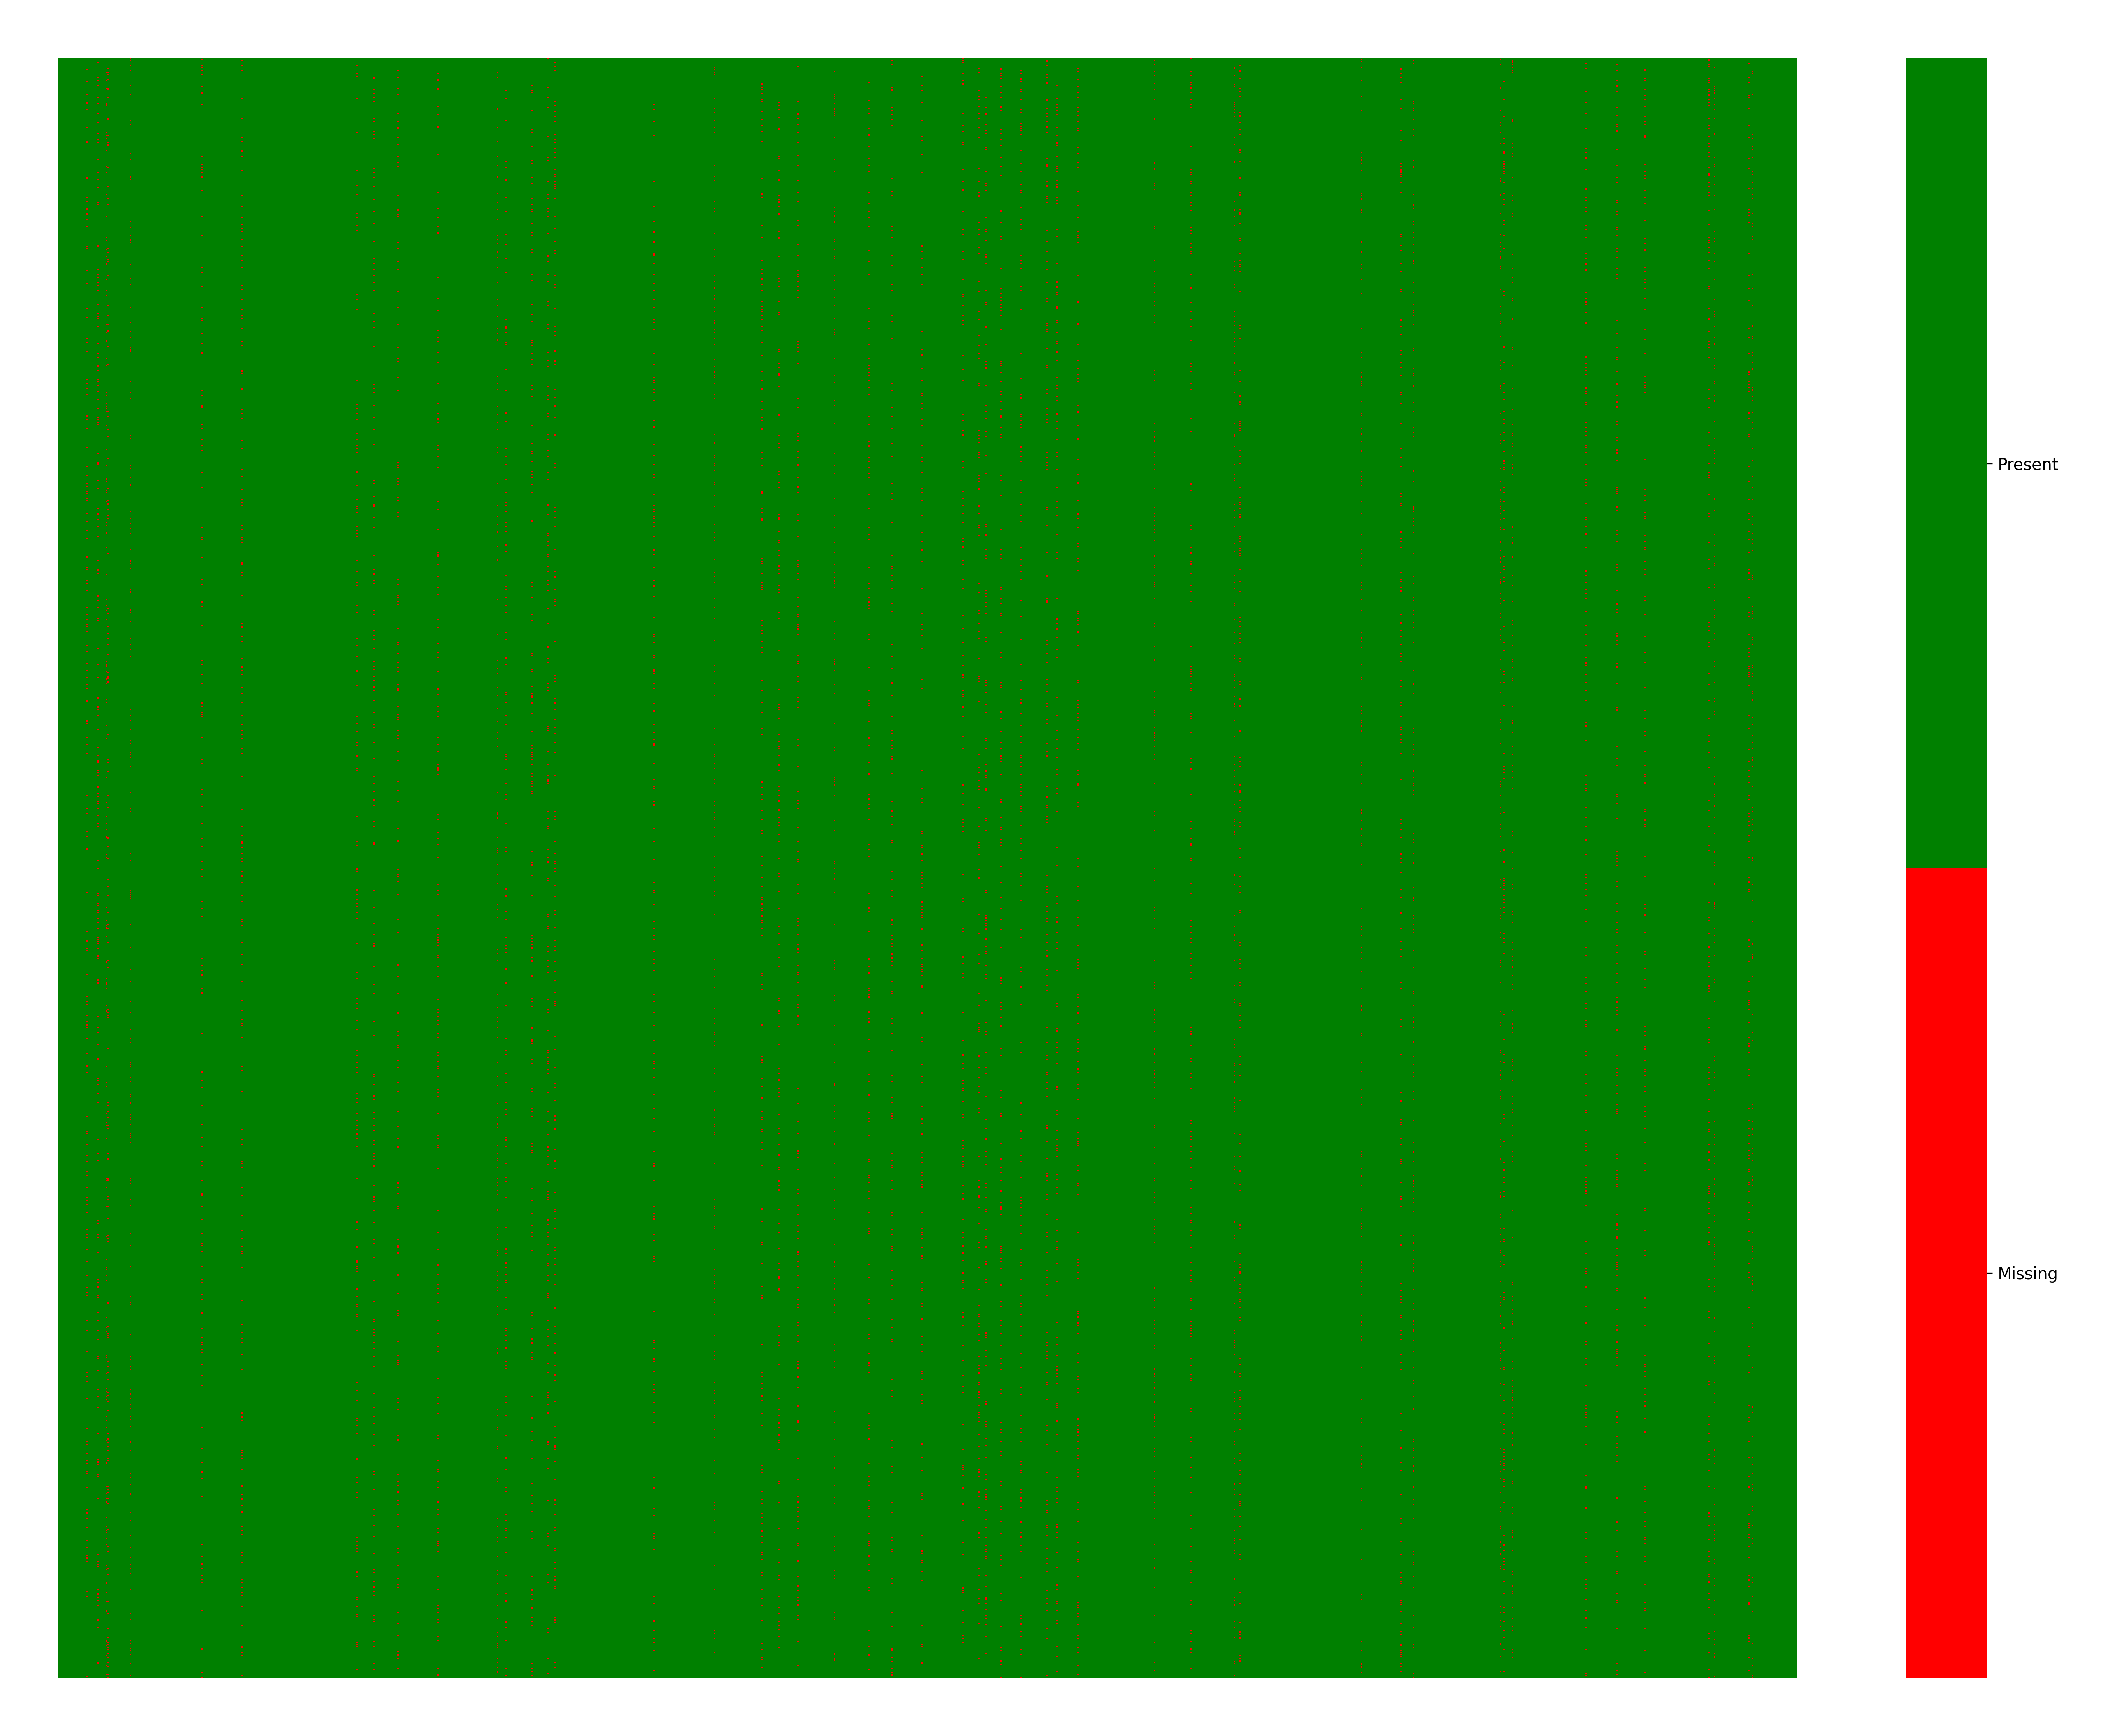
\includegraphics[width=\linewidth]{case1_heatmap_erased.png}
    \caption{Case 1 Input Dataset}
\end{figure}

\begin{figure}[H]
    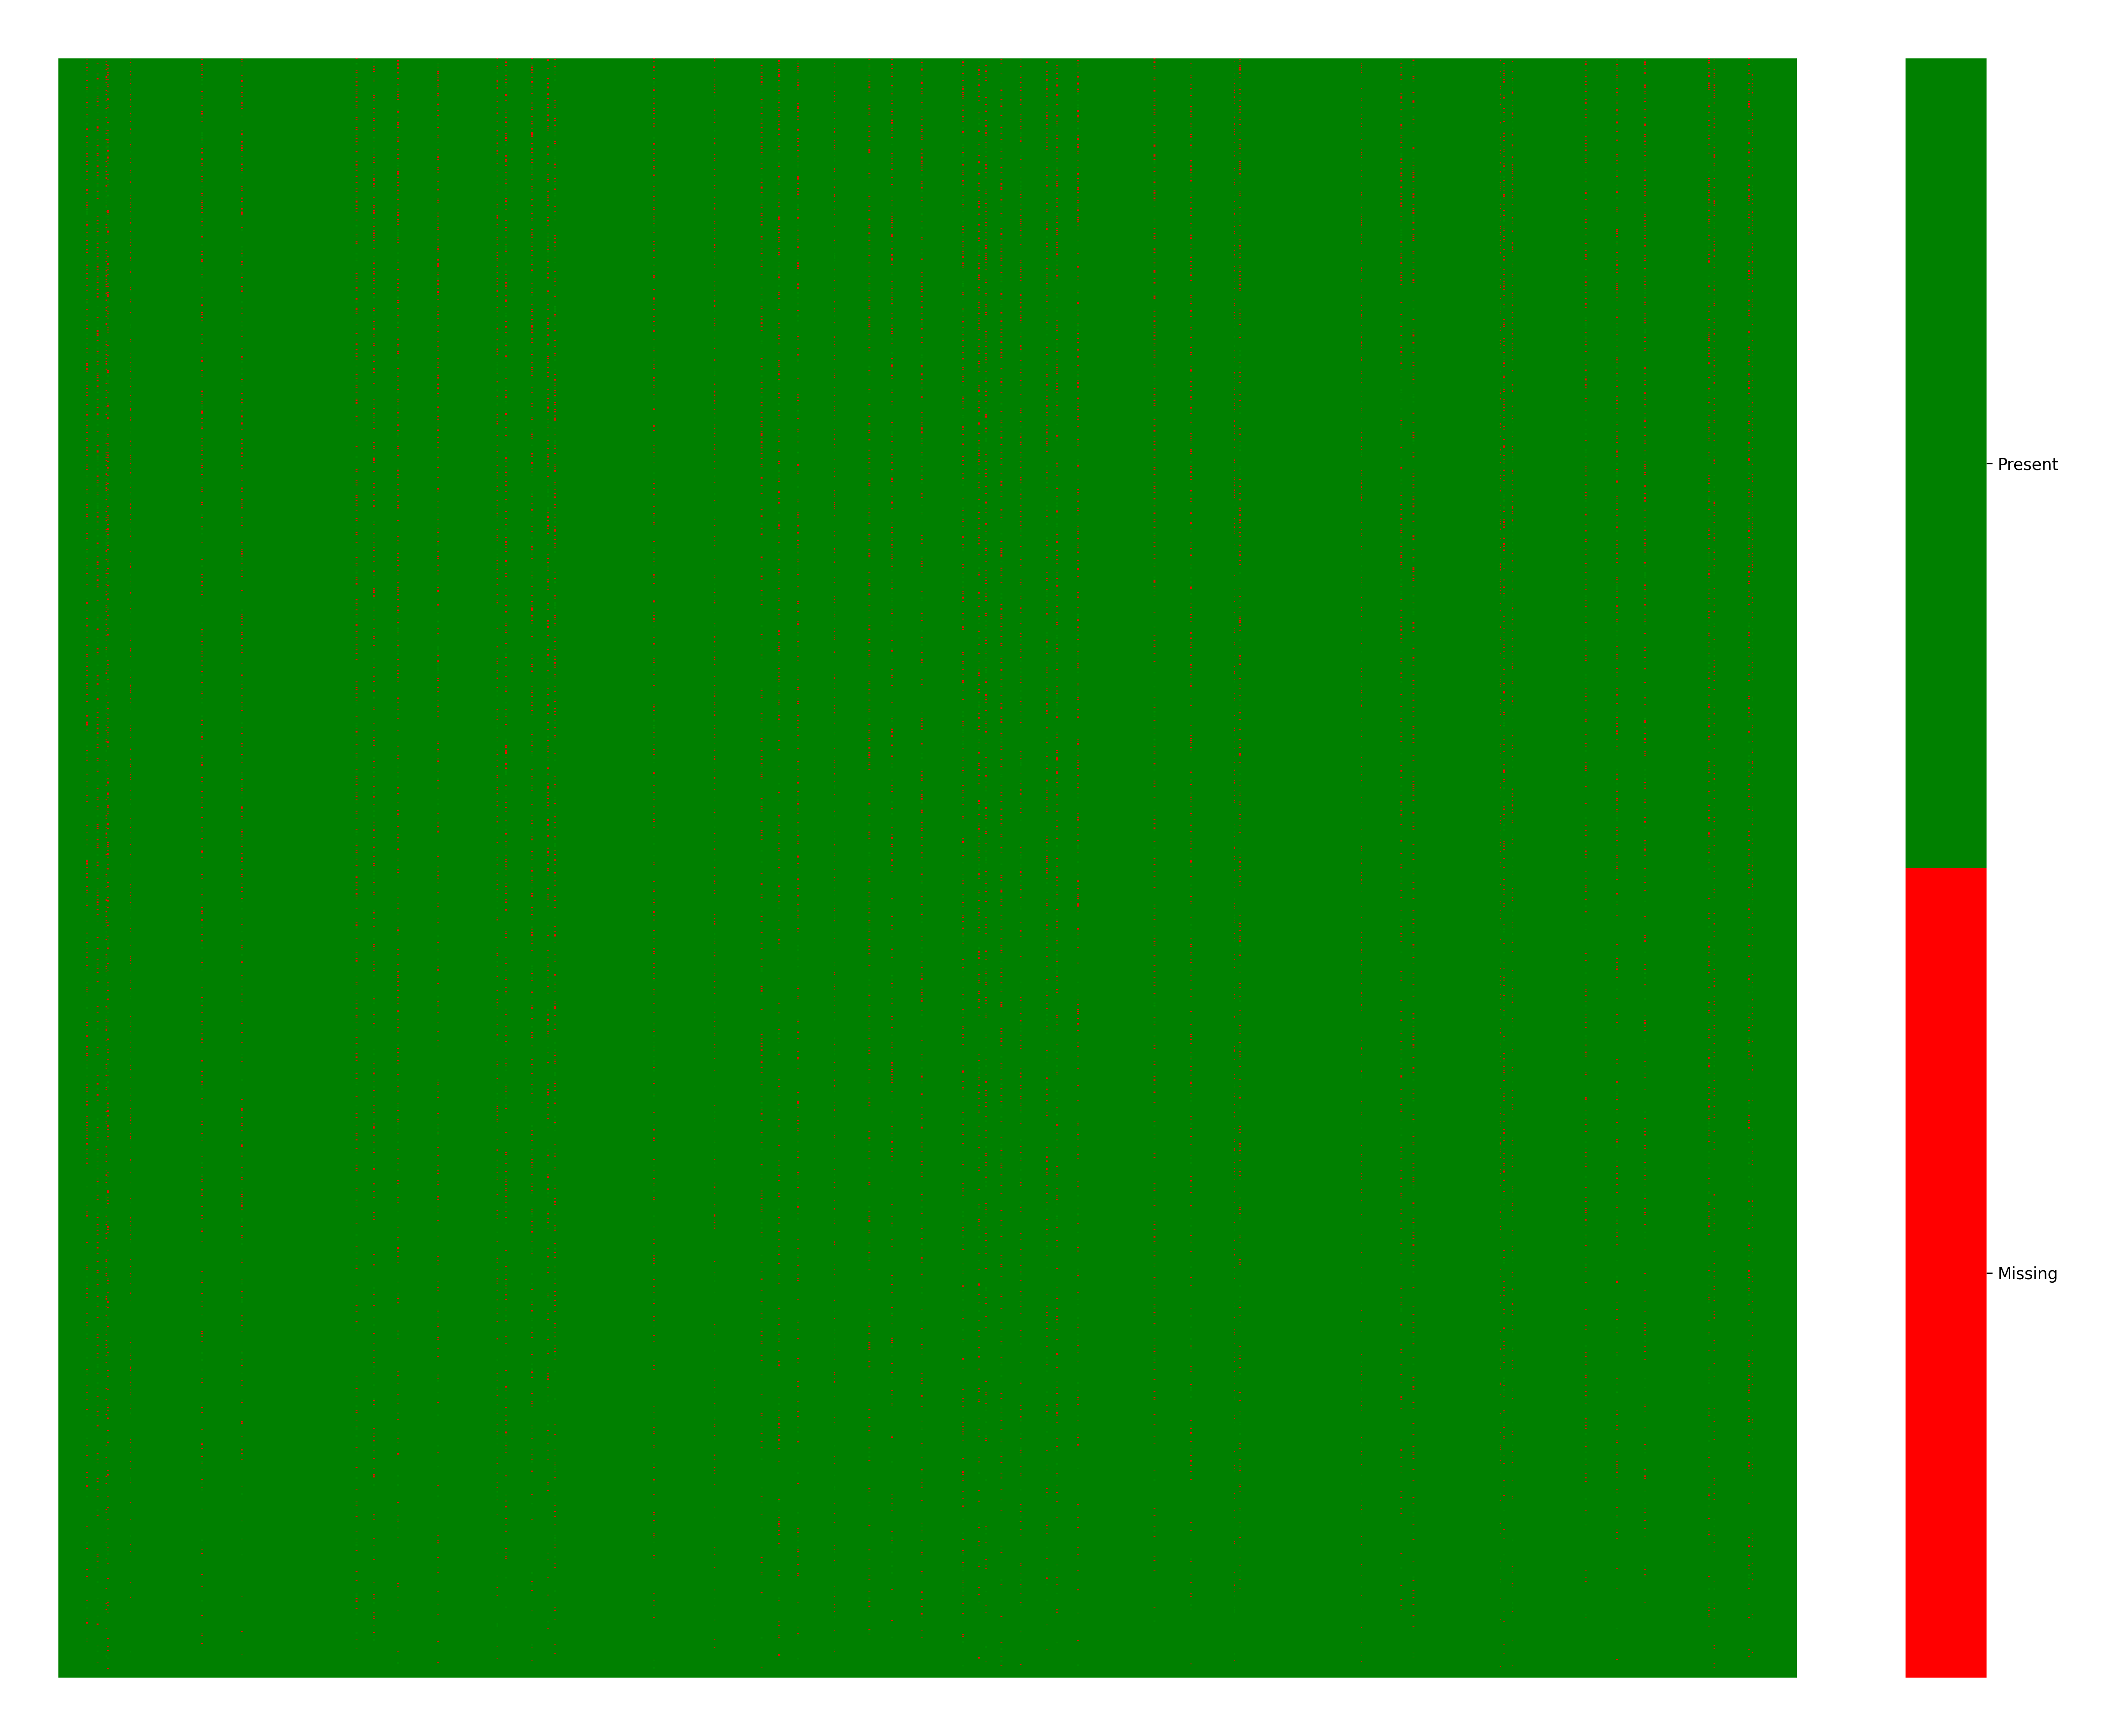
\includegraphics[width=\linewidth]{case1_v0.0_heatmap_cleaned.png}
    \caption*{Case 1 v0.0}
\end{figure}

\begin{figure}[H]
    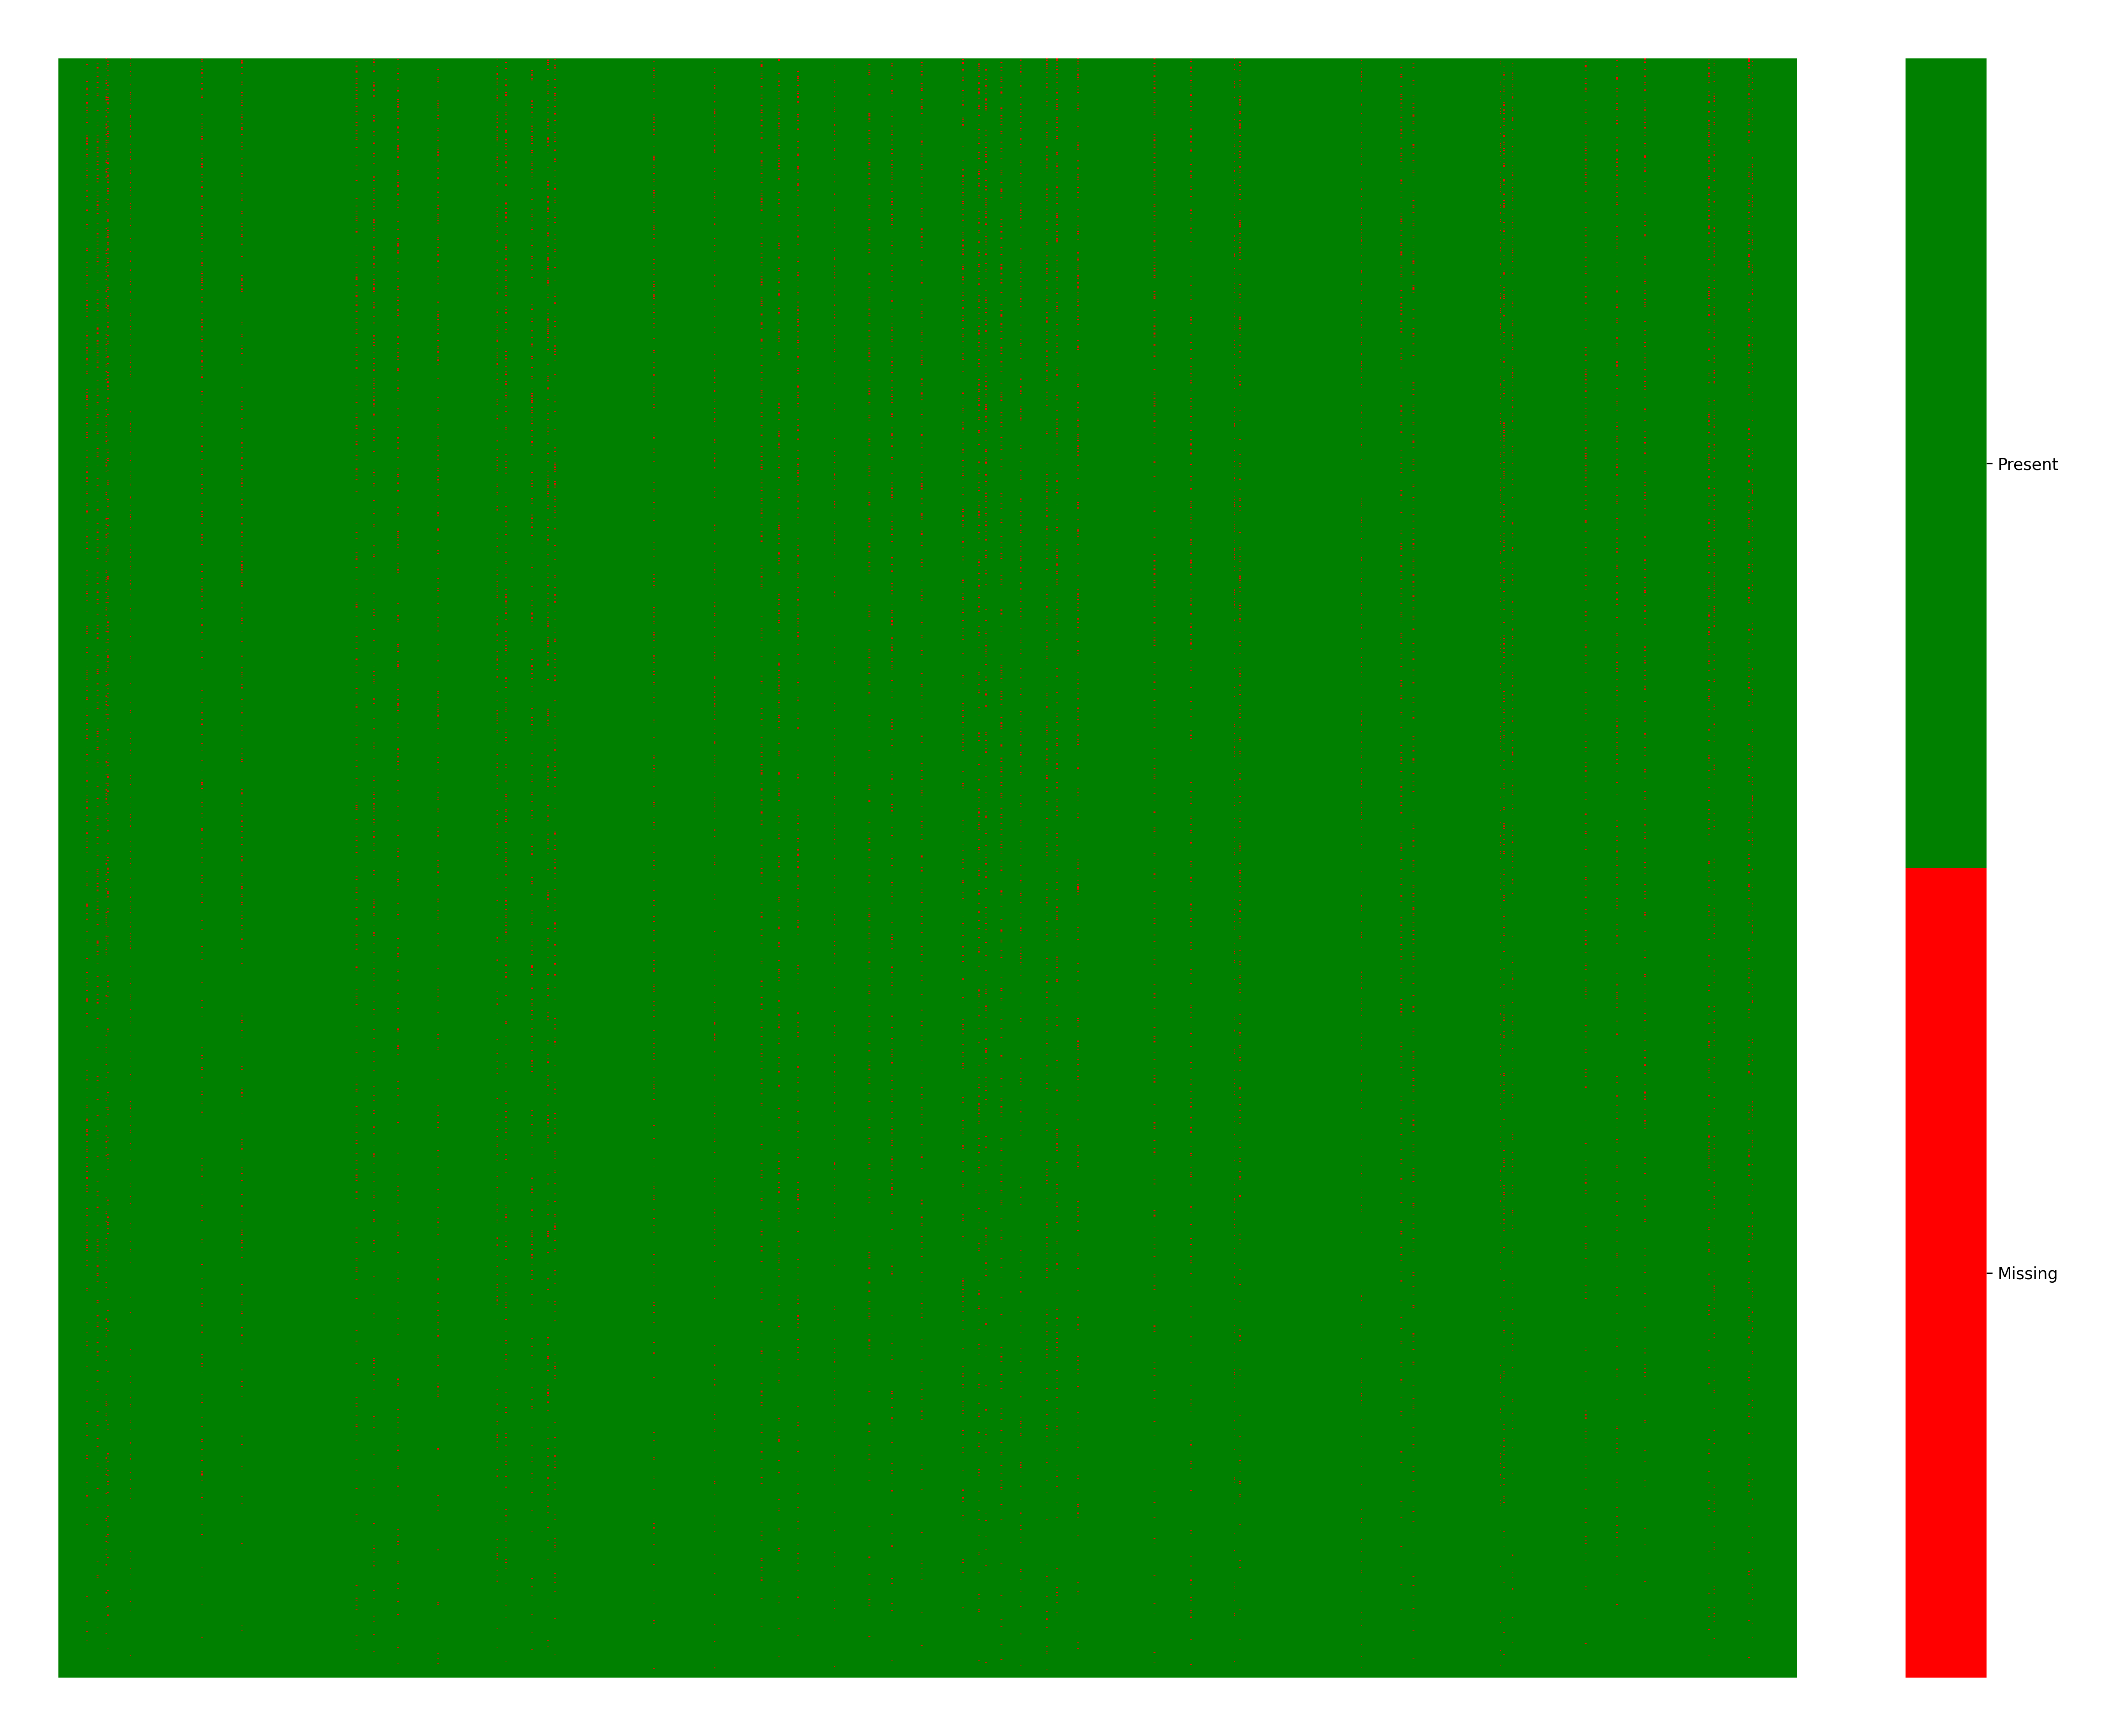
\includegraphics[width=\linewidth]{case1_v0.1_heatmap_cleaned.png}
    \caption*{Case 1 v0.1}
\end{figure}

\begin{figure}[H]
    \includegraphics[width=\linewidth]{case1_v0.2_heatmap_cleaned.png}
    \caption*{Case 1 v0.2}
\end{figure}

\begin{figure}[H]
    \includegraphics[width=\linewidth]{case1_v0.3_heatmap_cleaned.png}
    \caption*{Case 1 v0.3}
\end{figure}

\begin{figure}[H]
    \includegraphics[width=\linewidth]{case1_v0.4_heatmap_cleaned.png}
    \caption*{Case 1 v0.4}
\end{figure}

\begin{figure}[H]
    \includegraphics[width=\linewidth]{case1_v0.5_heatmap_cleaned.png}
    \caption*{Case 1 v0.5}
\end{figure}

\begin{figure}[H]
    \includegraphics[width=\linewidth]{case1_bnb_heatmap_cleaned.png}
    \caption*{Case 1 BnB}
\end{figure}

\textbf{Case 2:}
\begin{figure}[H]
    \centering
    \includegraphics[width=\linewidth]{case2_heatmap_erased.png}
    \caption*{Case 2 Input Dataset}
\end{figure}

\begin{figure}[H]
    \includegraphics[width=\linewidth]{case2_v0.0_heatmap_cleaned.png}
    \caption*{Case 2 v0.0}
\end{figure}

\begin{figure}[H]
    \includegraphics[width=\linewidth]{case2_v0.1_heatmap_cleaned.png}
    \caption*{Case 2 v0.1}
\end{figure}

\begin{figure}[H]
    \includegraphics[width=\linewidth]{case2_v0.2_heatmap_cleaned.png}
    \caption*{Case 2 v0.2}
\end{figure}

\begin{figure}[H]
    \includegraphics[width=\linewidth]{case2_v0.3_heatmap_cleaned.png}
    \caption*{Case 2 v0.3}
\end{figure}

\begin{figure}[H]
    \includegraphics[width=\linewidth]{case2_v0.4_heatmap_cleaned.png}
    \caption*{Case 2 v0.4}
\end{figure}

\begin{figure}[H]
    \includegraphics[width=\linewidth]{case2_v0.5_heatmap_cleaned.png}
    \caption*{Case 2 v0.5}
\end{figure}

\begin{figure}[H]
    \includegraphics[width=\linewidth]{case2_bnb_heatmap_cleaned.png}
    \caption*{Case 2 BnB}
\end{figure}

\textbf{Case 3:}
\begin{figure}[H]
    \centering
    \includegraphics[width=\linewidth]{case3_heatmap_erased.png}
    \caption*{Case 3 Input Dataset}
\end{figure}

\begin{figure}[H]
    \includegraphics[width=\linewidth]{case3_v0.0_heatmap_cleaned.png}
    \caption*{Case 3 v0.0}
\end{figure}

\begin{figure}[H]
    \includegraphics[width=\linewidth]{case3_v0.1_heatmap_cleaned.png}
    \caption*{Case 3 v0.1}
\end{figure}

\begin{figure}[H]
    \includegraphics[width=\linewidth]{case3_v0.2_heatmap_cleaned.png}
    \caption*{Case 3 v0.2}
\end{figure}

\begin{figure}[H]
    \includegraphics[width=\linewidth]{case3_v0.3_heatmap_cleaned.png}
    \caption*{Case 3 v0.3}
\end{figure}

\begin{figure}[H]
    \includegraphics[width=\linewidth]{case3_v0.4_heatmap_cleaned.png}
    \caption*{Case 3 v0.4}
\end{figure}

\begin{figure}[H]
    \includegraphics[width=\linewidth]{case3_v0.5_heatmap_cleaned.png}
    \caption*{Case 3 v0.5}
\end{figure}

\begin{figure}[H]
    \includegraphics[width=\linewidth]{case3_bnb_heatmap_cleaned.png}
    \caption*{Case 3 BnB}
\end{figure}

\textbf{Case 4:}
\begin{figure}[H]
    \centering
    \includegraphics[width=\linewidth]{case4_heatmap_erased.png}
    \caption*{Case 4 Input Dataset}
\end{figure}

\begin{figure}[H]
    \includegraphics[width=\linewidth]{case4_v0.0_heatmap_cleaned.png}
    \caption*{Case 4 v0.0}
\end{figure}

\begin{figure}[H]
    \includegraphics[width=\linewidth]{case4_v0.1_heatmap_cleaned.png}
    \caption*{Case 4 v0.1}
\end{figure}

\begin{figure}[H]
    \includegraphics[width=\linewidth]{case4_v0.2_heatmap_cleaned.png}
    \caption*{Case 4 v0.2}
\end{figure}

\begin{figure}[H]
    \includegraphics[width=\linewidth]{case4_v0.3_heatmap_cleaned.png}
    \caption*{Case 4 v0.3}
\end{figure}

\begin{figure}[H]
    \includegraphics[width=\linewidth]{case4_v0.4_heatmap_cleaned.png}
    \caption*{Case 4 v0.4}
\end{figure}

\begin{figure}[H]
    \includegraphics[width=\linewidth]{case4_v0.5_heatmap_cleaned.png}
    \caption*{Case 4 v0.5}
\end{figure}

\begin{figure}[H]
    \includegraphics[width=\linewidth]{case4_bnb_heatmap_cleaned.png}
    \caption*{Case 4 BnB}
\end{figure}

\textbf{Case 5:}
\begin{figure}[H]
    \centering
    \includegraphics[width=\linewidth]{case5_heatmap_erased.png}
    \caption*{Case 5 Input Dataset}
\end{figure}

\begin{figure}[H]
    \includegraphics[width=\linewidth]{case5_v0.0_heatmap_cleaned.png}
    \caption*{Case 5 v0.0}
\end{figure}

\begin{figure}[H]
    \includegraphics[width=\linewidth]{case5_v0.1_heatmap_cleaned.png}
    \caption*{Case 5 v0.1}
\end{figure}

\begin{figure}[H]
    \includegraphics[width=\linewidth]{case5_v0.2_heatmap_cleaned.png}
    \caption*{Case 5 v0.2}
\end{figure}

\begin{figure}[H]
    \includegraphics[width=\linewidth]{case5_v0.3_heatmap_cleaned.png}
    \caption*{Case 5 v0.3}
\end{figure}

\begin{figure}[H]
    \includegraphics[width=\linewidth]{case5_v0.4_heatmap_cleaned.png}
    \caption*{Case 5 v0.4}
\end{figure}

\begin{figure}[H]
    \includegraphics[width=\linewidth]{case5_v0.5_heatmap_cleaned.png}
    \caption*{Case 5 v0.5}
\end{figure}

\begin{figure}[H]
    \includegraphics[width=\linewidth]{case5_bnb_heatmap_cleaned.png}
    \caption*{Case 5 BnB}
\end{figure}

\textbf{Case 6:}
\begin{figure}[H]
    \centering
    \includegraphics[width=\linewidth]{case6_heatmap_erased.png}
    \caption*{Case 6 Input Dataset}
\end{figure}

\begin{figure}[H]
    \includegraphics[width=\linewidth]{case6_v0.0_heatmap_cleaned.png}
    \caption*{Case 6 v0.0}
\end{figure}

\begin{figure}[H]
    \includegraphics[width=\linewidth]{case6_v0.1_heatmap_cleaned.png}
    \caption*{Case 6 v0.1}
\end{figure}

\begin{figure}[H]
    \includegraphics[width=\linewidth]{case6_v0.2_heatmap_cleaned.png}
    \caption*{Case 6 v0.2}
\end{figure}

\begin{figure}[H]
    \includegraphics[width=\linewidth]{case6_v0.3_heatmap_cleaned.png}
    \caption*{Case 6 v0.3}
\end{figure}

\begin{figure}[H]
    \includegraphics[width=\linewidth]{case6_v0.4_heatmap_cleaned.png}
    \caption*{Case 6 v0.4}
\end{figure}

\begin{figure}[H]
    \includegraphics[width=\linewidth]{case6_v0.5_heatmap_cleaned.png}
    \caption*{Case 6 v0.5}
\end{figure}

\begin{figure}[H]
    \includegraphics[width=\linewidth]{case6_bnb_heatmap_cleaned.png}
    \caption*{Case 6 BnB}
\end{figure}

\textbf{Case 7:}
\begin{figure}[H]
    \centering
    \includegraphics[width=\linewidth]{case8_heatmap_erased.png}
    \caption*{Case 7 Input Dataset}
\end{figure}

\begin{figure}[H]
    \includegraphics[width=\linewidth]{case8_v0.0_heatmap_cleaned.png}
    \caption*{Case 7 v0.0}
\end{figure}

\begin{figure}[H]
    \includegraphics[width=\linewidth]{case8_v0.1_heatmap_cleaned.png}
    \caption*{Case 7 v0.1}
\end{figure}

\begin{figure}[H]
    \includegraphics[width=\linewidth]{case8_v0.2_heatmap_cleaned.png}
    \caption*{Case 7 v0.2}
\end{figure}

\begin{figure}[H]
    \includegraphics[width=\linewidth]{case8_v0.3_heatmap_cleaned.png}
    \caption*{Case 7 v0.3}
\end{figure}

\begin{figure}[H]
    \includegraphics[width=\linewidth]{case8_v0.4_heatmap_cleaned.png}
    \caption*{Case 7 v0.4}
\end{figure}

\begin{figure}[H]
    \includegraphics[width=\linewidth]{case8_v0.5_heatmap_cleaned.png}
    \caption*{Case 7 v0.5}
\end{figure}

\begin{figure}[H]
    \includegraphics[width=\linewidth]{case8_bnb_heatmap_cleaned.png}
    \caption*{Case 7 BnB}
\end{figure}

\textbf{Case 8:}
\begin{figure}[H]
    \centering
    \includegraphics[width=\linewidth]{case9_heatmap_erased.png}
    \caption*{Case 8 Input Dataset}
\end{figure}

\begin{figure}[H]
    \includegraphics[width=\linewidth]{case9_v0.0_heatmap_cleaned.png}
    \caption*{Case 8 v0.0}
\end{figure}

\begin{figure}[H]
    \includegraphics[width=\linewidth]{case9_v0.1_heatmap_cleaned.png}
    \caption*{Case 8 v0.1}
\end{figure}

\begin{figure}[H]
    \includegraphics[width=\linewidth]{case9_v0.2_heatmap_cleaned.png}
    \caption*{Case 8 v0.2}
\end{figure}

\begin{figure}[H]
    \includegraphics[width=\linewidth]{case9_v0.3_heatmap_cleaned.png}
    \caption*{Case 8 v0.3}
\end{figure}

\begin{figure}[H]
    \includegraphics[width=\linewidth]{case9_v0.4_heatmap_cleaned.png}
    \caption*{Case 8 v0.4}
\end{figure}

\begin{figure}[H]
    \includegraphics[width=\linewidth]{case9_v0.5_heatmap_cleaned.png}
    \caption*{Case 8 v0.5}
\end{figure}

\begin{figure}[H]
    \includegraphics[width=\linewidth]{case9_bnb_heatmap_cleaned.png}
    \caption*{Case 8 BnB}
\end{figure}

\textbf{Case 9:}
\begin{figure}[H]
    \centering
    \includegraphics[width=\linewidth]{case10_heatmap_erased.png}
    \caption*{Case 9 Input Dataset}
\end{figure}

\begin{figure}[H]
    \includegraphics[width=\linewidth]{case10_v0.0_heatmap_cleaned.png}
    \caption*{Case 9 v0.0}
\end{figure}

\begin{figure}[H]
    \includegraphics[width=\linewidth]{case10_v0.1_heatmap_cleaned.png}
    \caption*{Case 9 v0.1}
\end{figure}

\begin{figure}[H]
    \includegraphics[width=\linewidth]{case10_v0.2_heatmap_cleaned.png}
    \caption*{Case 9 v0.2}
\end{figure}

\begin{figure}[H]
    \includegraphics[width=\linewidth]{case10_v0.3_heatmap_cleaned.png}
    \caption*{Case 9 v0.3}
\end{figure}

\begin{figure}[H]
    \includegraphics[width=\linewidth]{case10_v0.4_heatmap_cleaned.png}
    \caption*{Case 9 v0.4}
\end{figure}

\begin{figure}[H]
    \includegraphics[width=\linewidth]{case10_v0.5_heatmap_cleaned.png}
    \caption*{Case 9 v0.5}
\end{figure}

\begin{figure}[H]
    \includegraphics[width=\linewidth]{case10_bnb_heatmap_cleaned.png}
    \caption*{Case 9 BnB}
\end{figure}



\newpage
\section{User Guide}
\lstinputlisting[caption=Project README]{README.md}
\lstinputlisting[caption=Project Dependencies]{requirements.txt}
\end{document}

